\documentclass{beamer}
\usetheme{Boadilla}
\usefonttheme{professionalfonts}
\usepackage{lmodern}
\usepackage{graphicx}
\usepackage[space]{grffile}
\usepackage{multicol}

\title{Inputs for MyLake-Sediment Model}
\subtitle{Lake Erie}
\author{I. Markelov, B. McNeil}
\institute{Ecohydrology}
\date{\today}

\graphicspath{ {../../post_proc_scripts/plots/} }

\begin{document}

\begin{frame}
\titlepage
\end{frame}


\begin{frame}
\begin{multicols}{2}
\tableofcontents
\end{multicols}
\end{frame}

\section{Weather}
\label{sec:weather}

\subsection{Western Basin}
\label{sub:wes}

\begin{frame}
\frametitle{Weather: Western Basin}
\begin{figure}
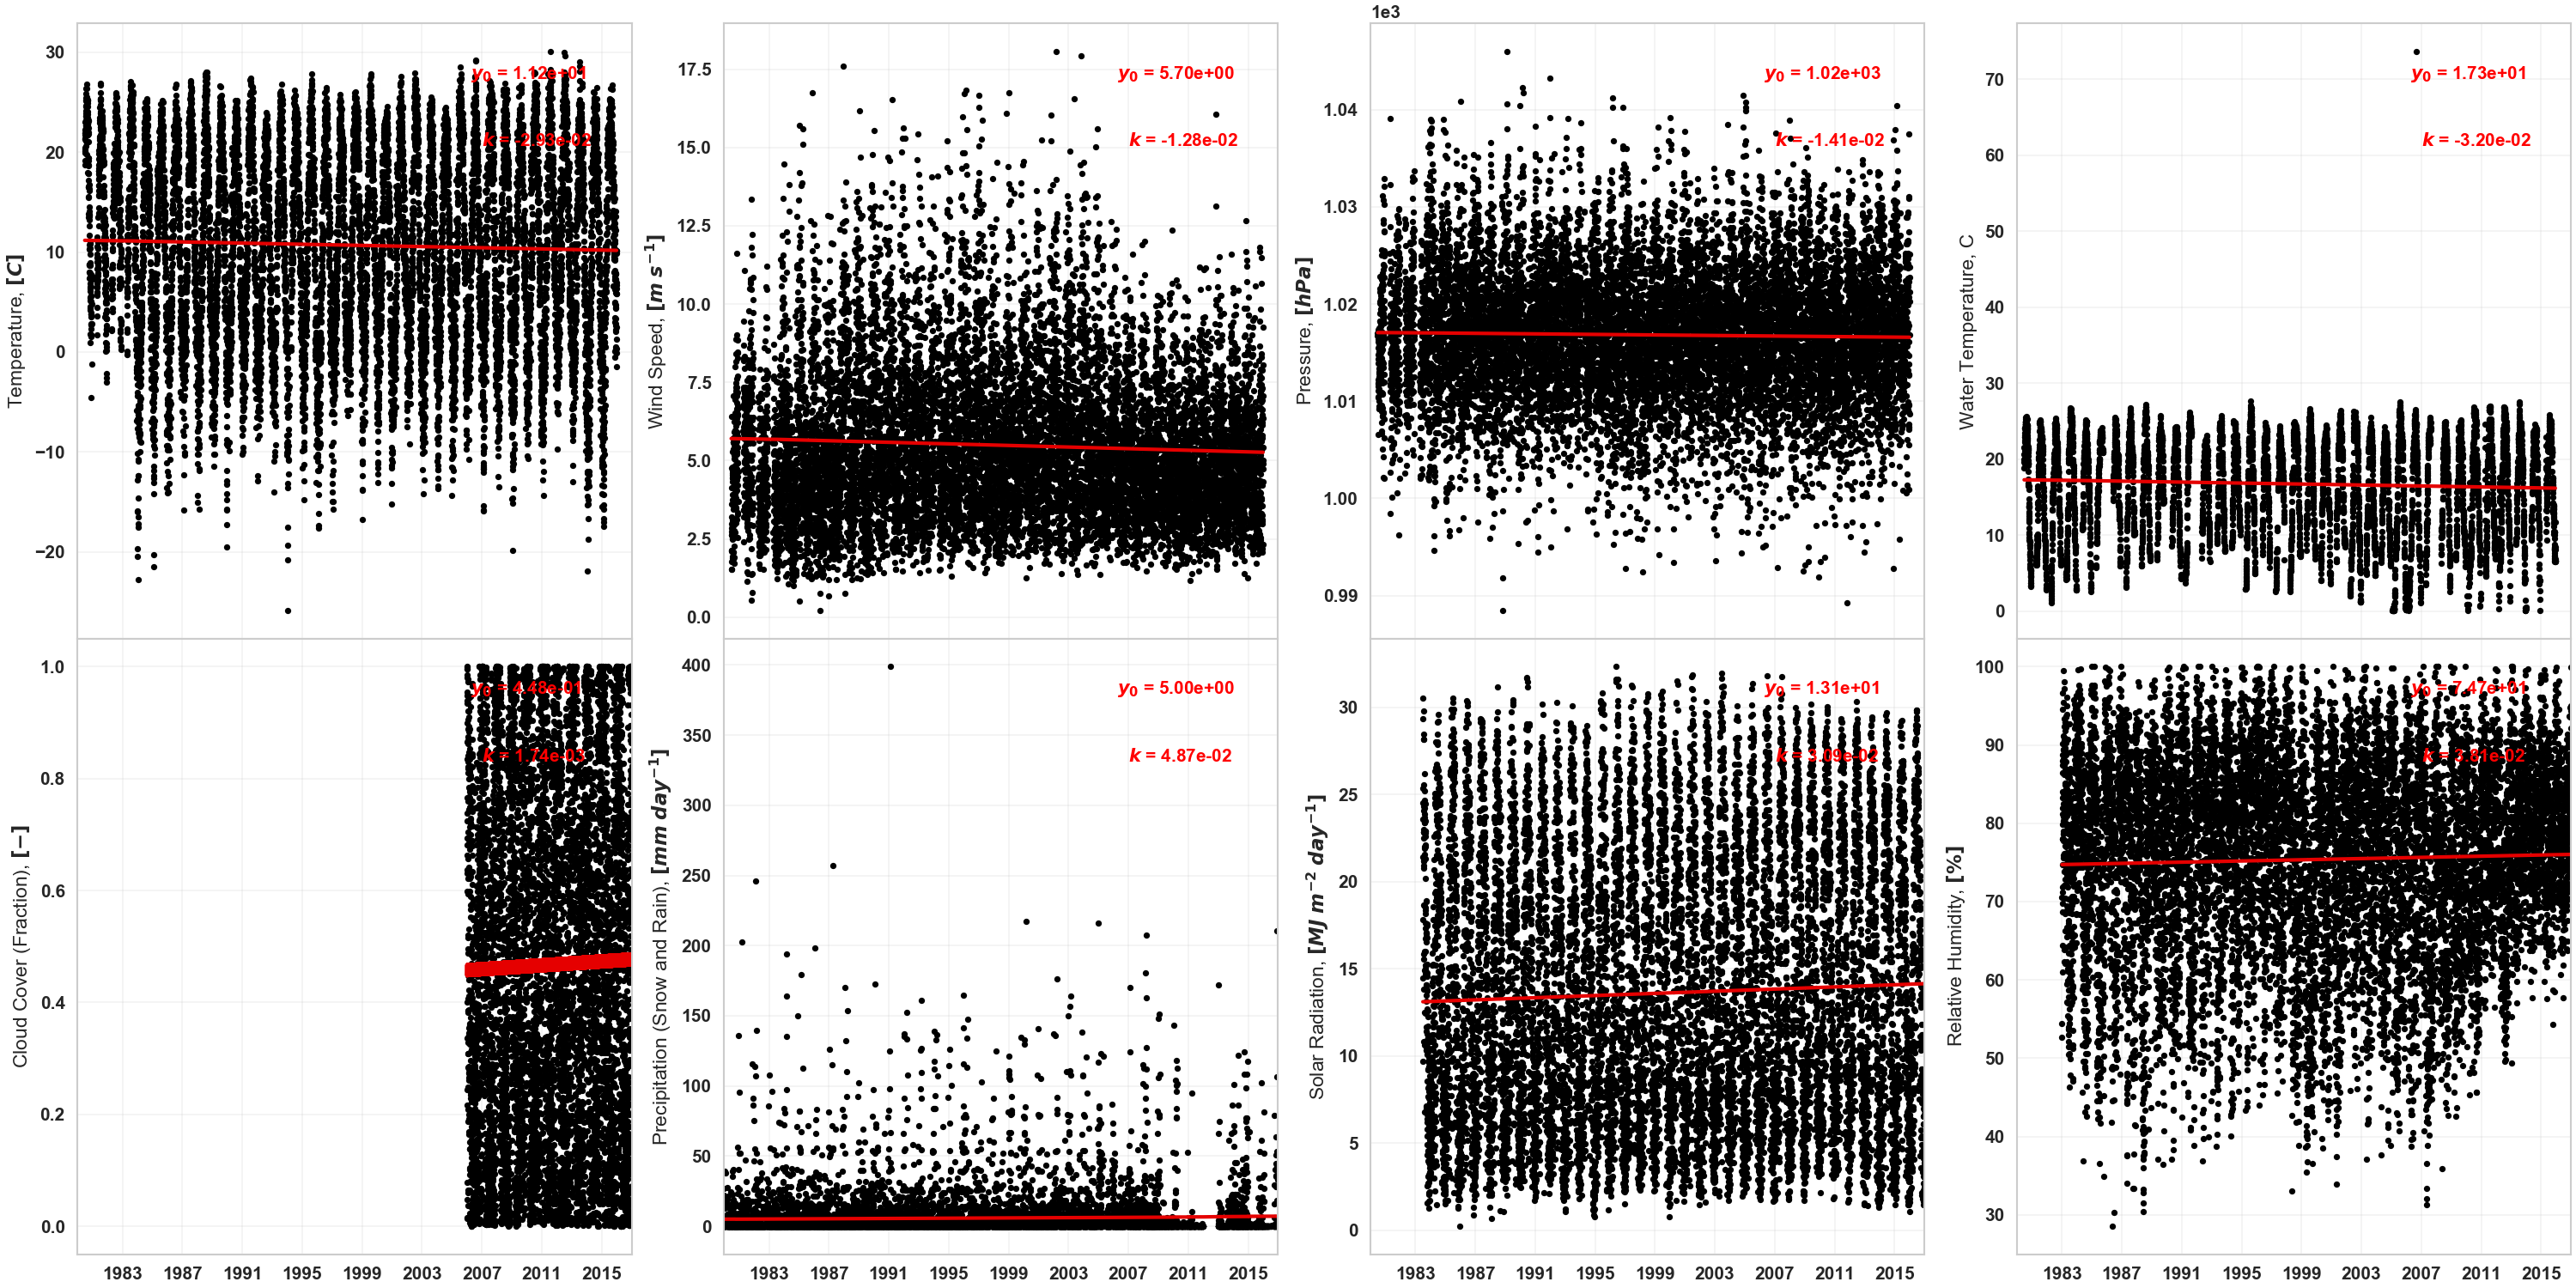
\includegraphics[width=\textwidth]{weather/western basin weather.png}
\end{figure}
\end{frame}

\subsection{Central Basin}
\label{sub:cen}

\begin{frame}
\frametitle{Weather: Central Basin}
\begin{figure}
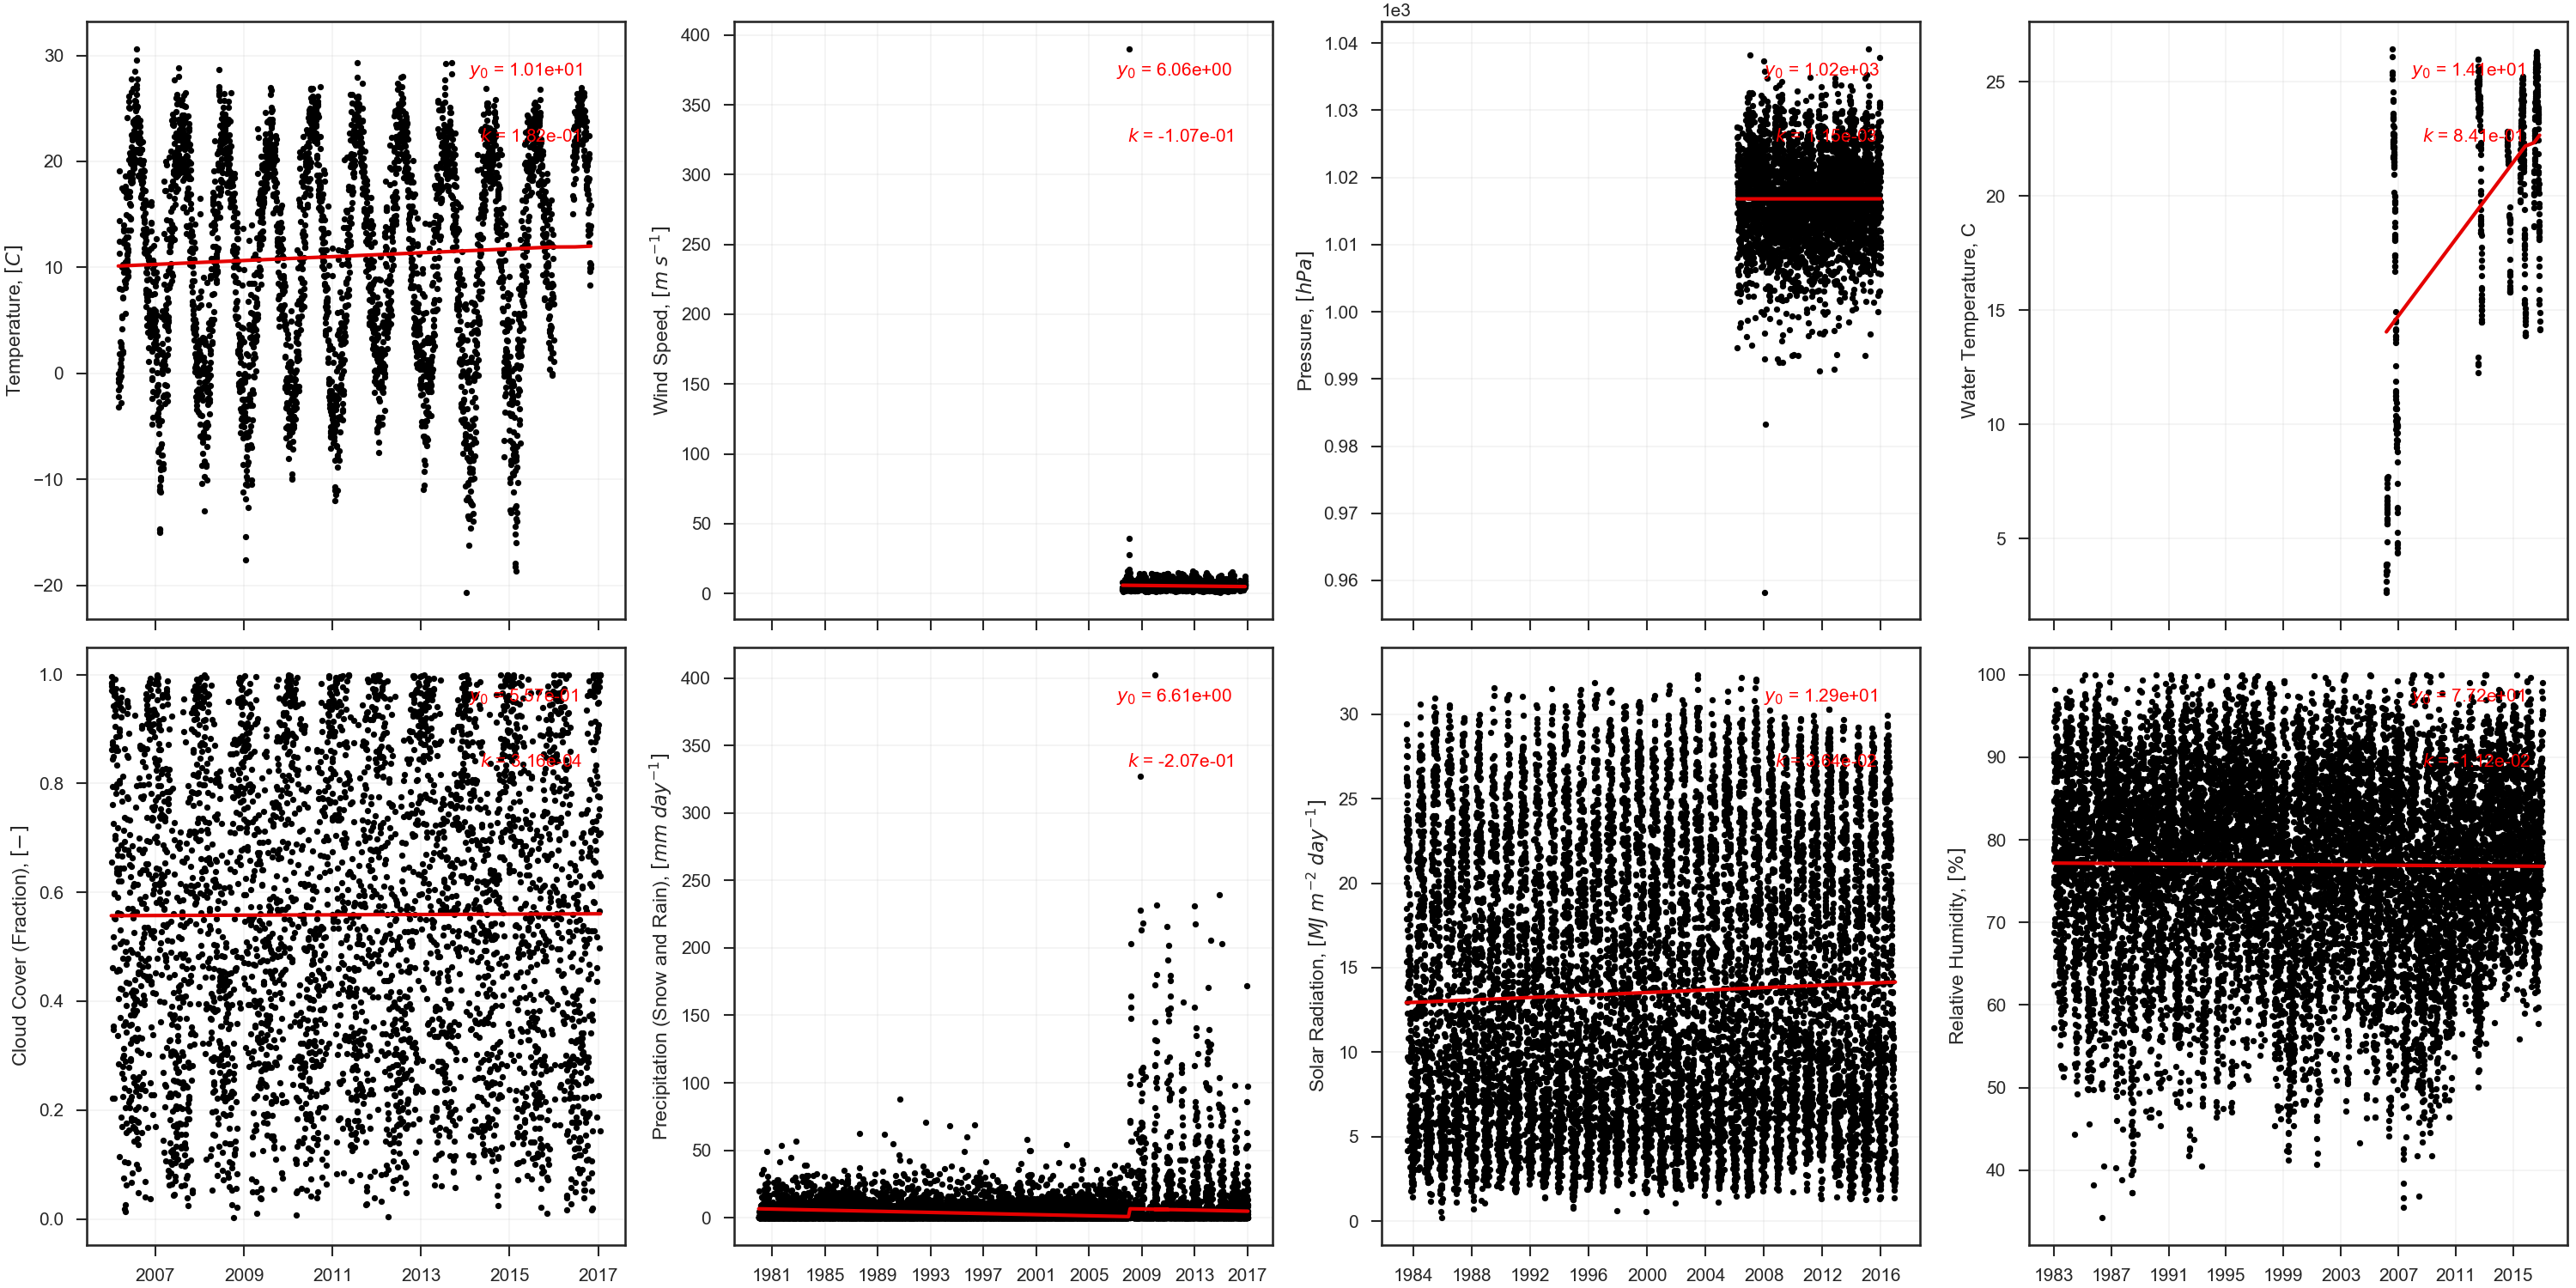
\includegraphics[width=\textwidth]{weather/central basin weather.png}
\end{figure}
\end{frame}

\subsection{Easter Basin}
\label{sub:wes}

\begin{frame}
\frametitle{Weather: Eastern Basin}
\begin{figure}
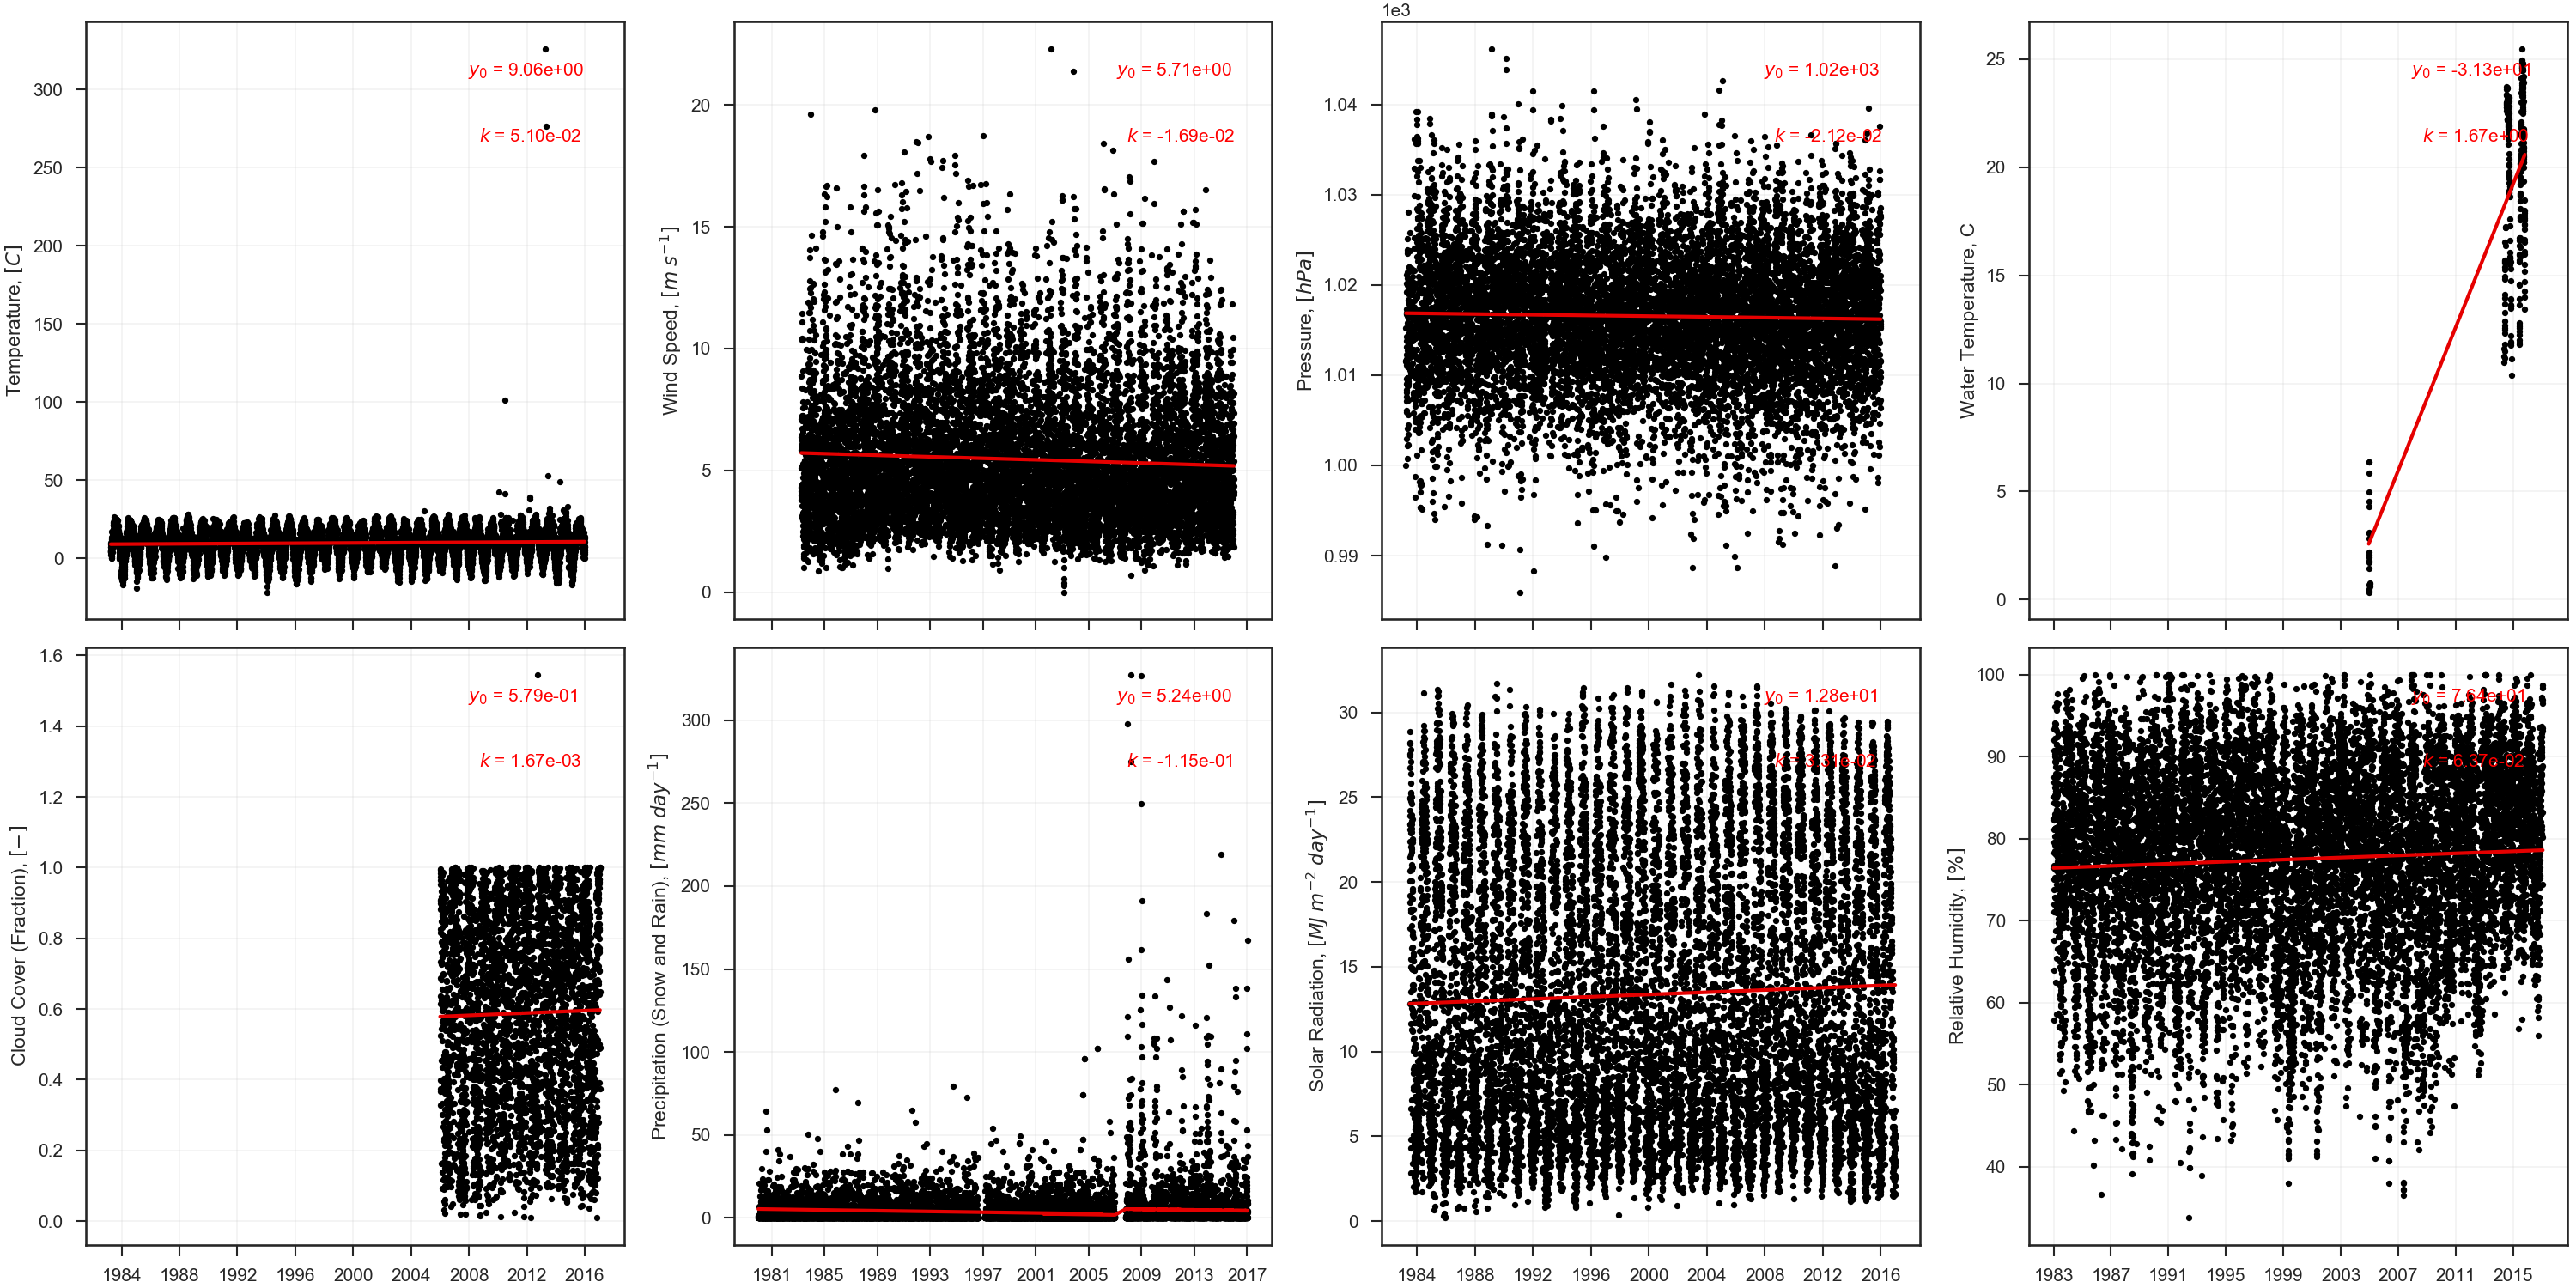
\includegraphics[width=\textwidth]{weather/eastern basin weather.png}
\end{figure}
\end{frame}

\section{US Rivers' Inputs}
\label{sec:river_inputs}

\subsection{Western Basin}
\label{sub:western_basin}

\begin{frame}
\frametitle{Western Basin: Detroit river}
\begin{figure}
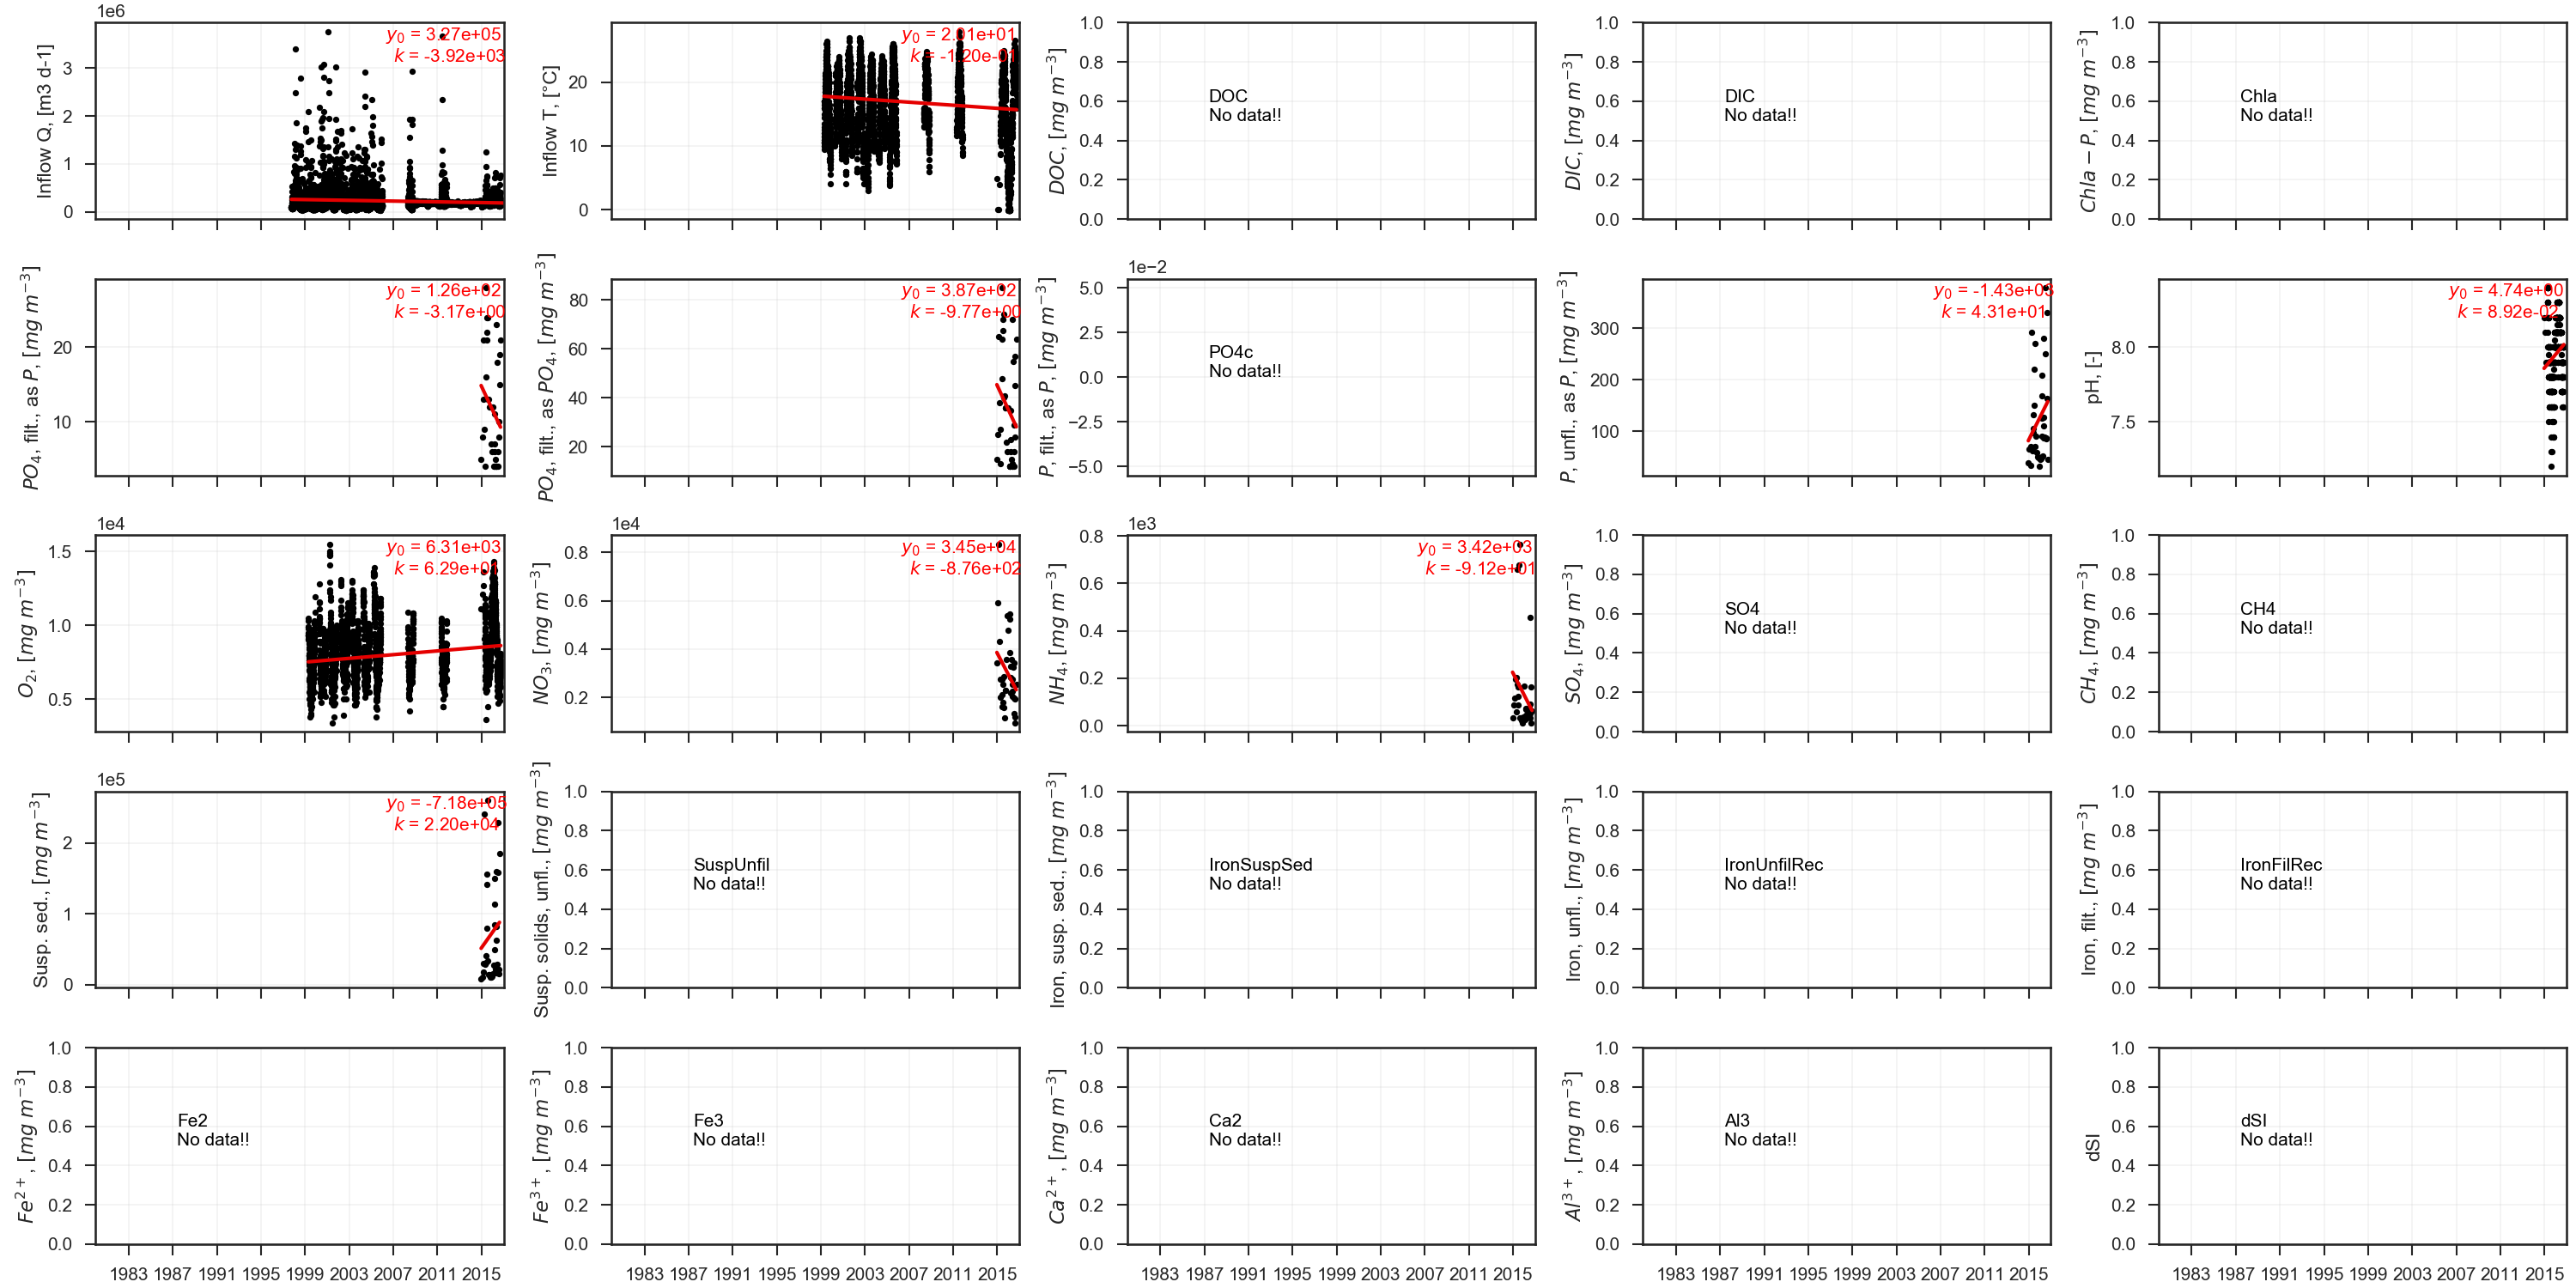
\includegraphics[width=\textwidth]{rivers/Western basin/plot_all detroitriver.png}
\end{figure}
\end{frame}


\begin{frame}
\frametitle{Western Basin: Huron river}
\begin{figure}
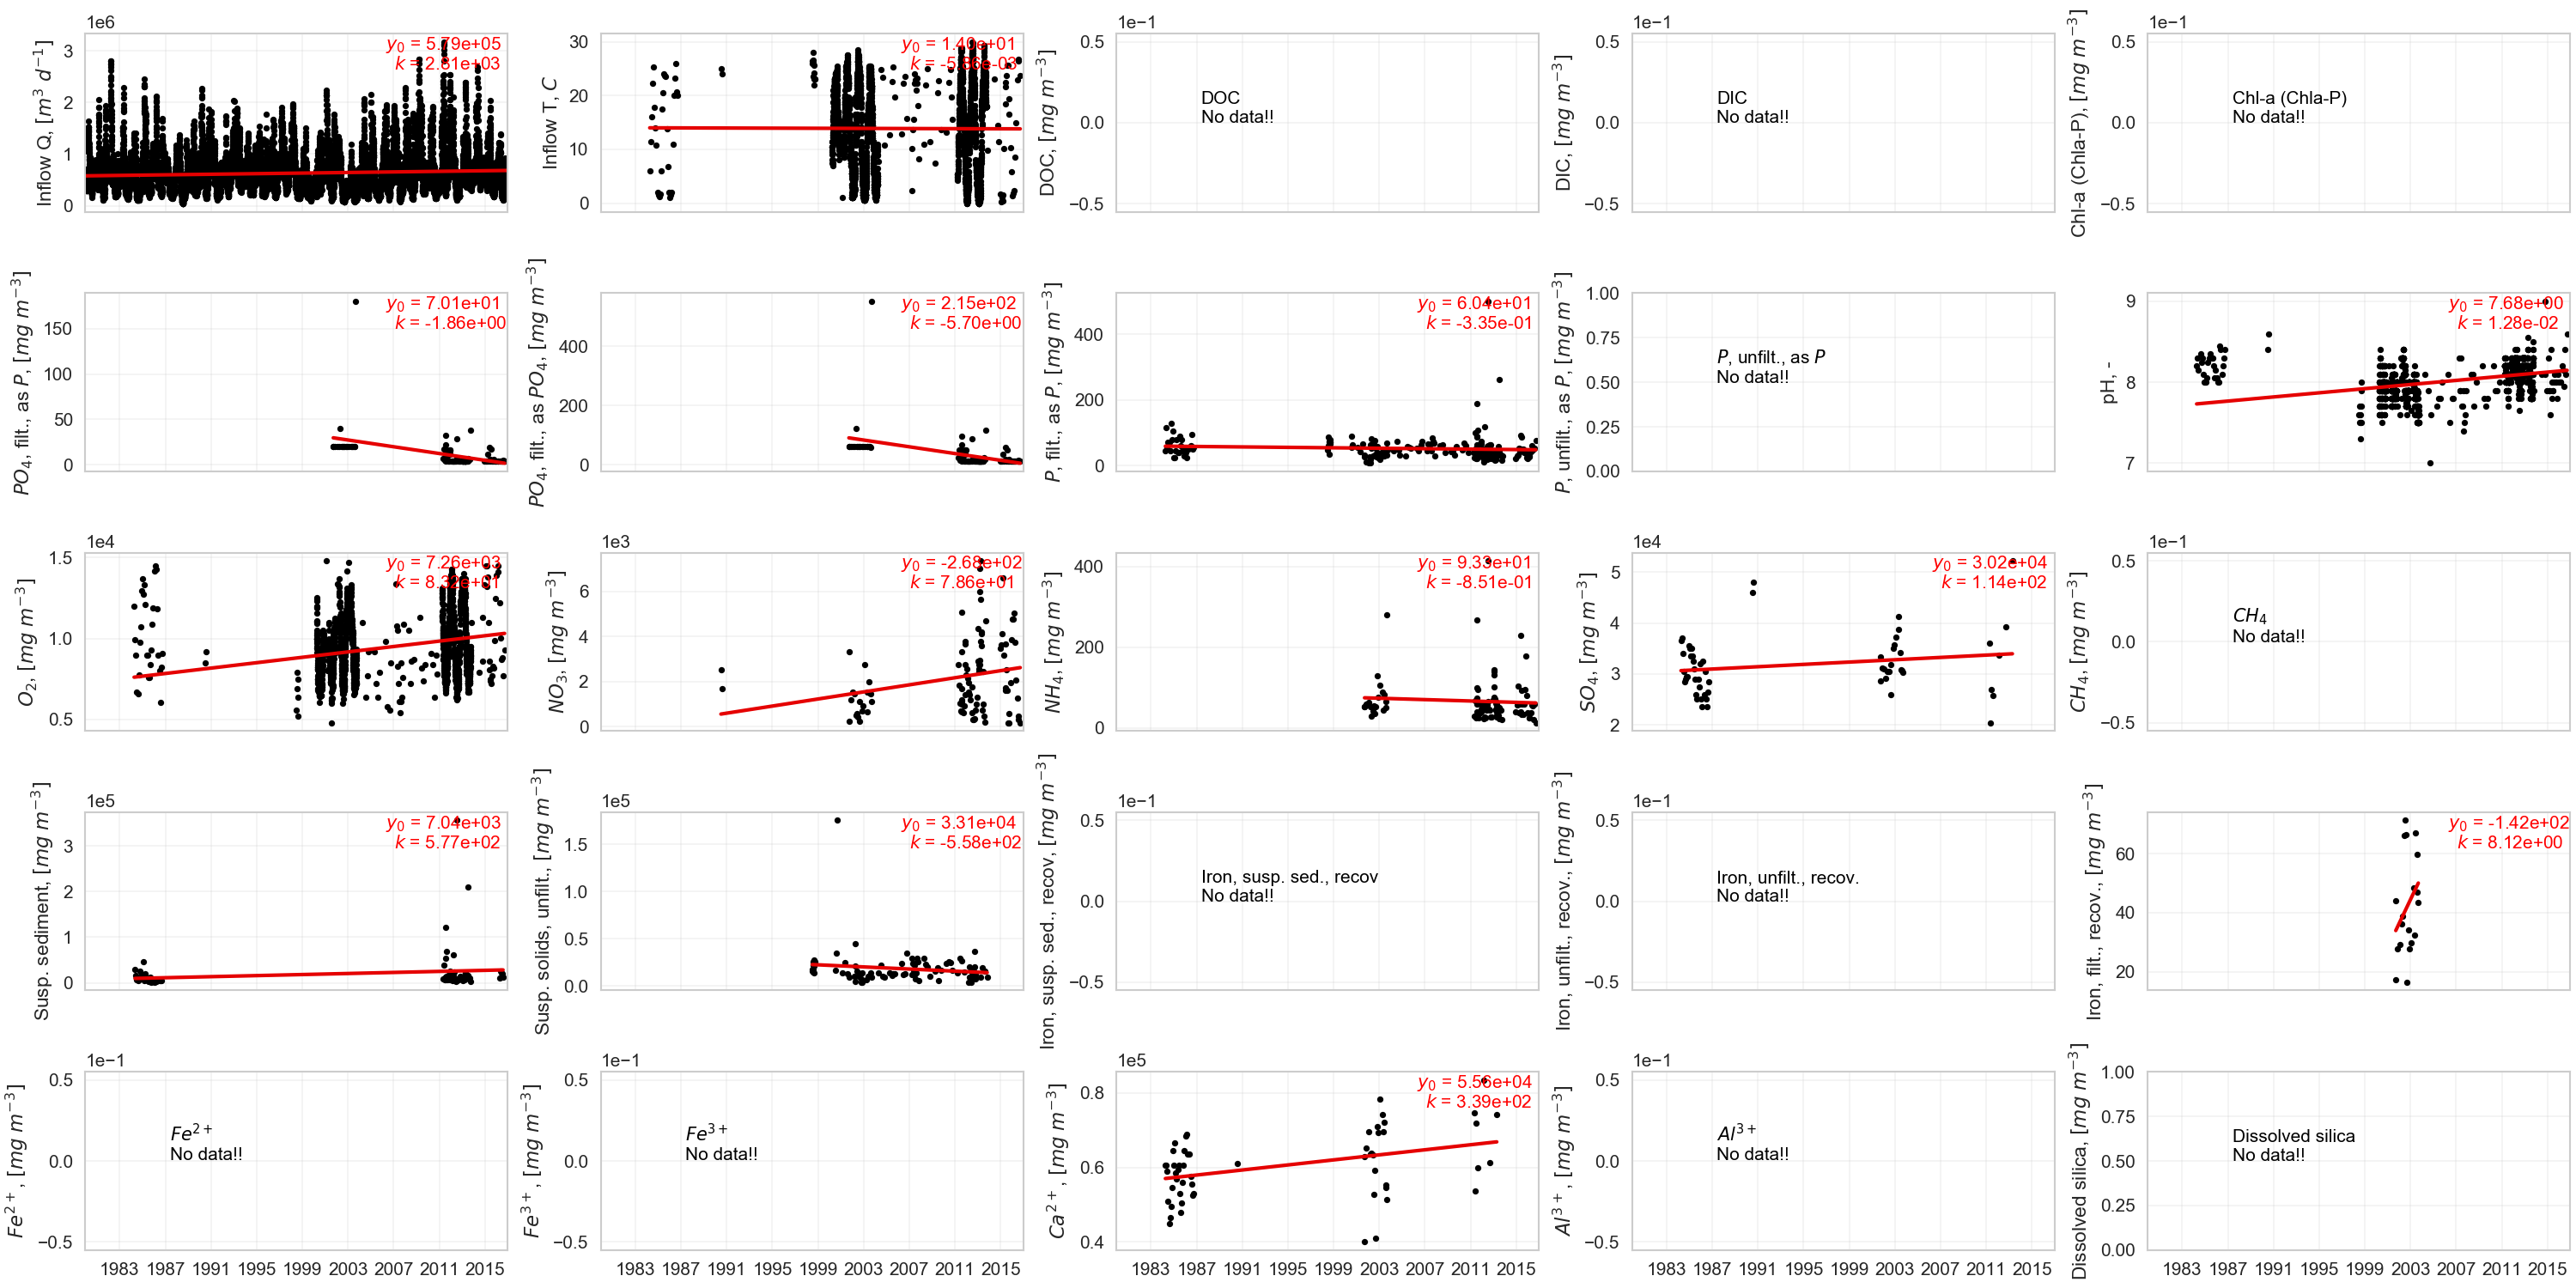
\includegraphics[width=\textwidth]{rivers/Western basin/plot_all huronriver.png}
\end{figure}
\end{frame}


\begin{frame}
\frametitle{Western Basin: Maumee river}
\begin{figure}
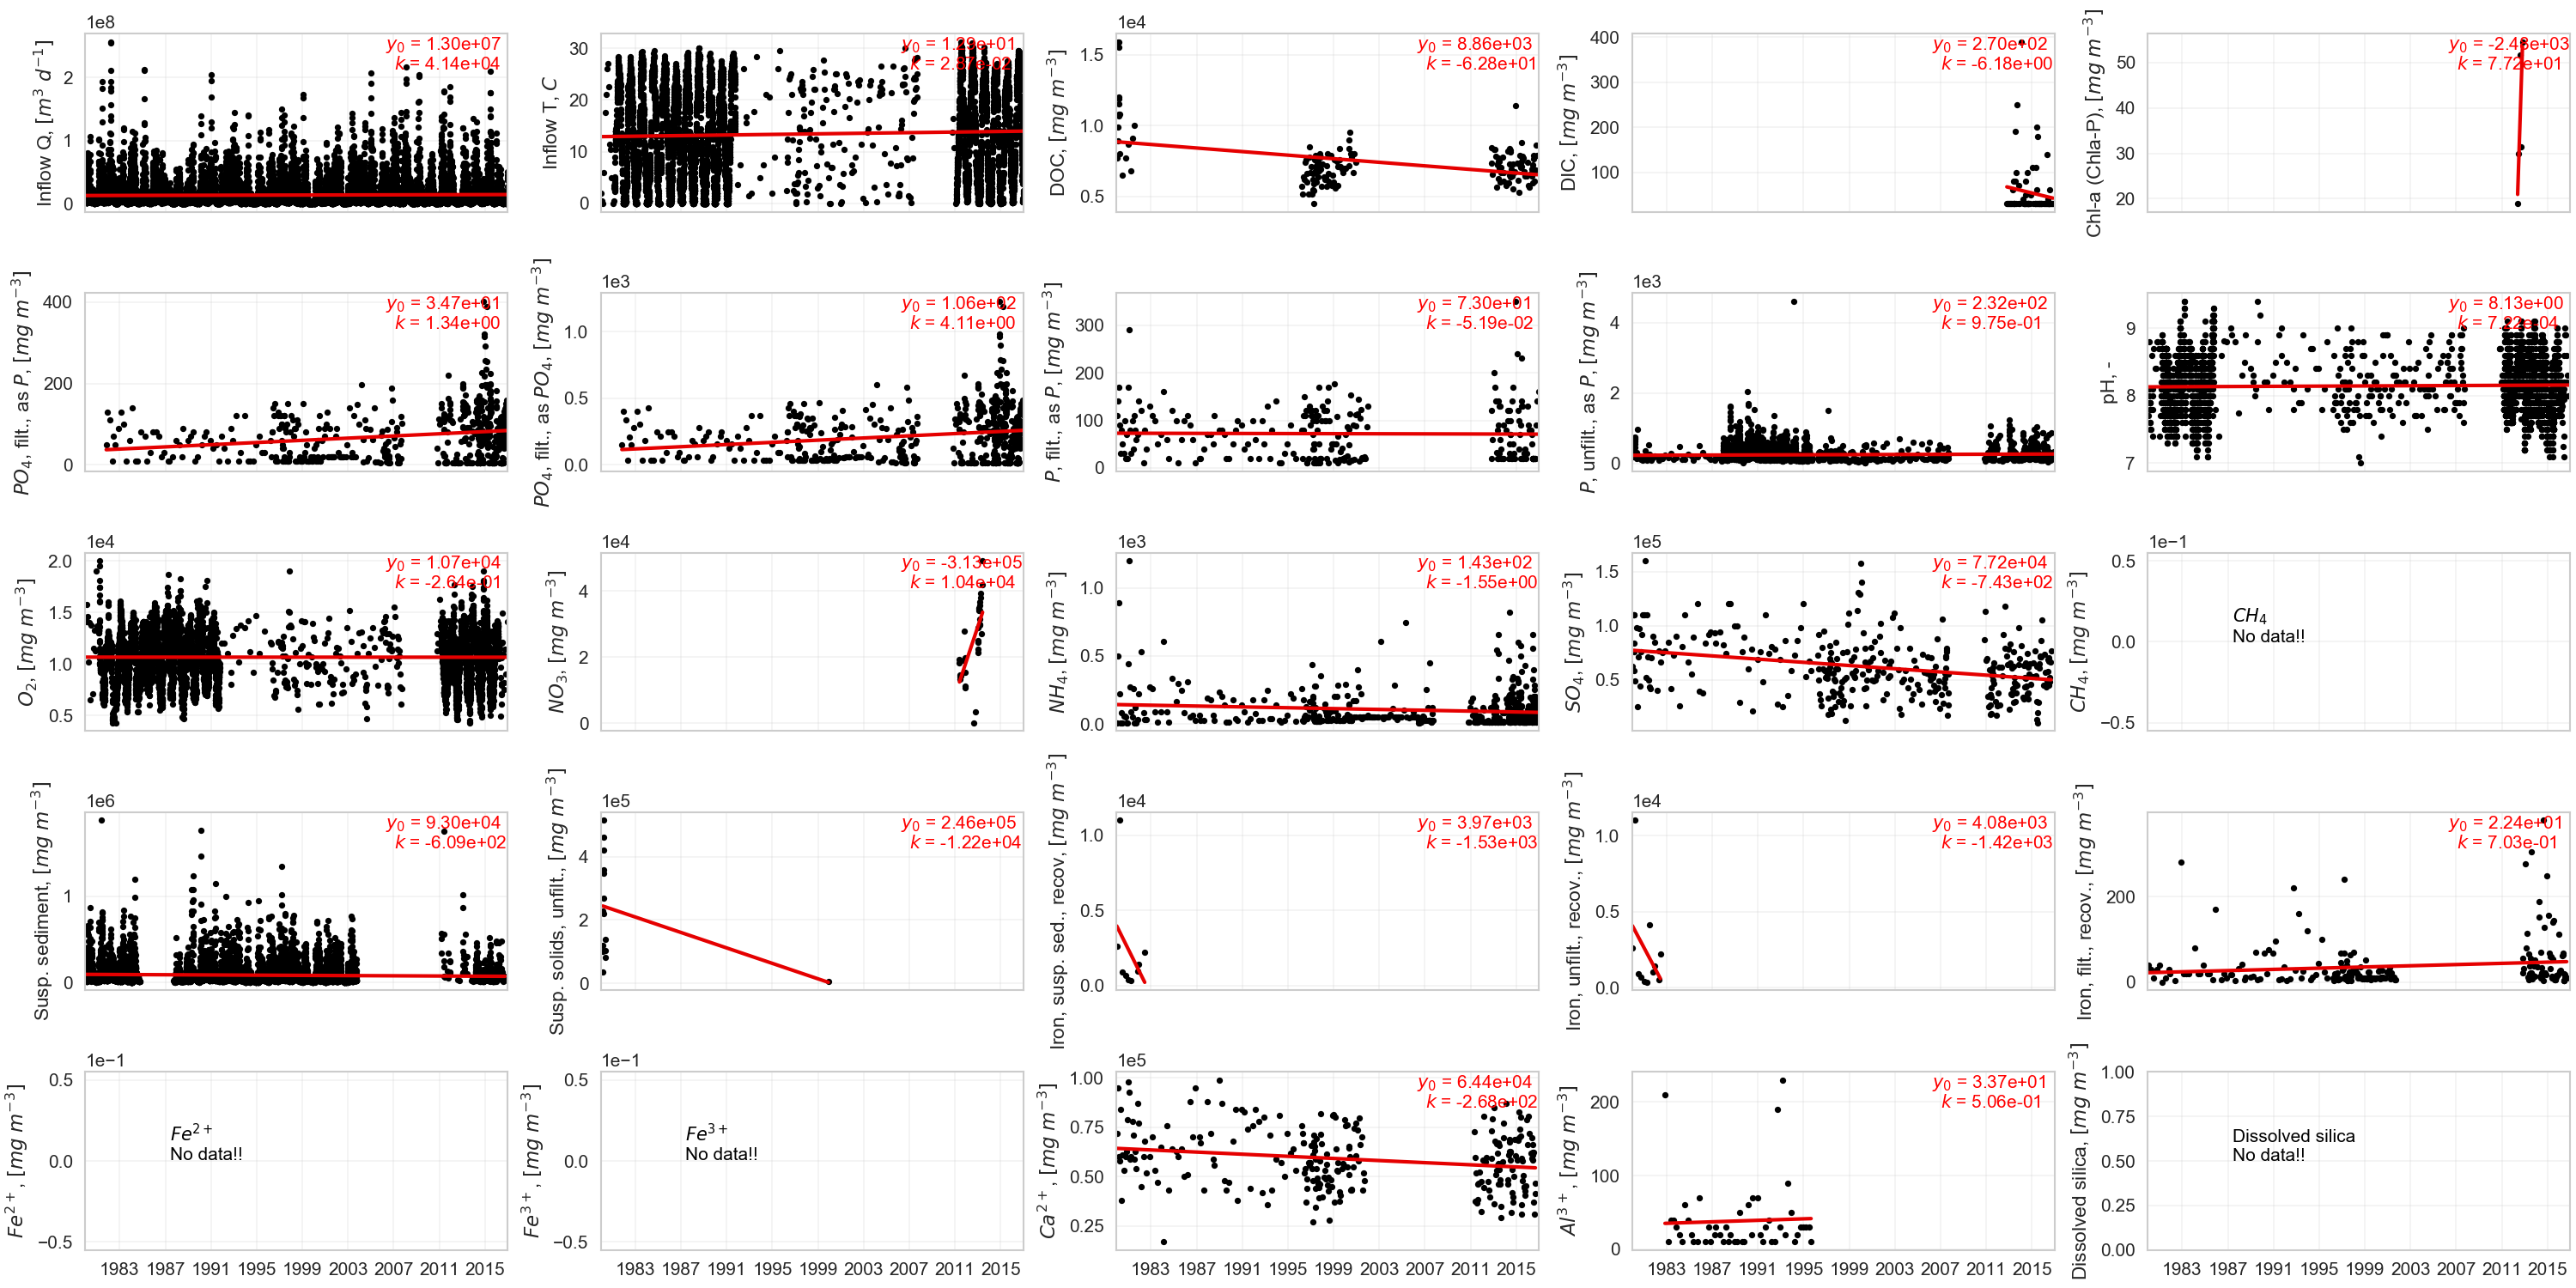
\includegraphics[width=\textwidth]{rivers/Western basin/plot_all maumeeriver.png}
\end{figure}
\end{frame}


\begin{frame}
\frametitle{Western Basin: Ottawa river}
\begin{figure}
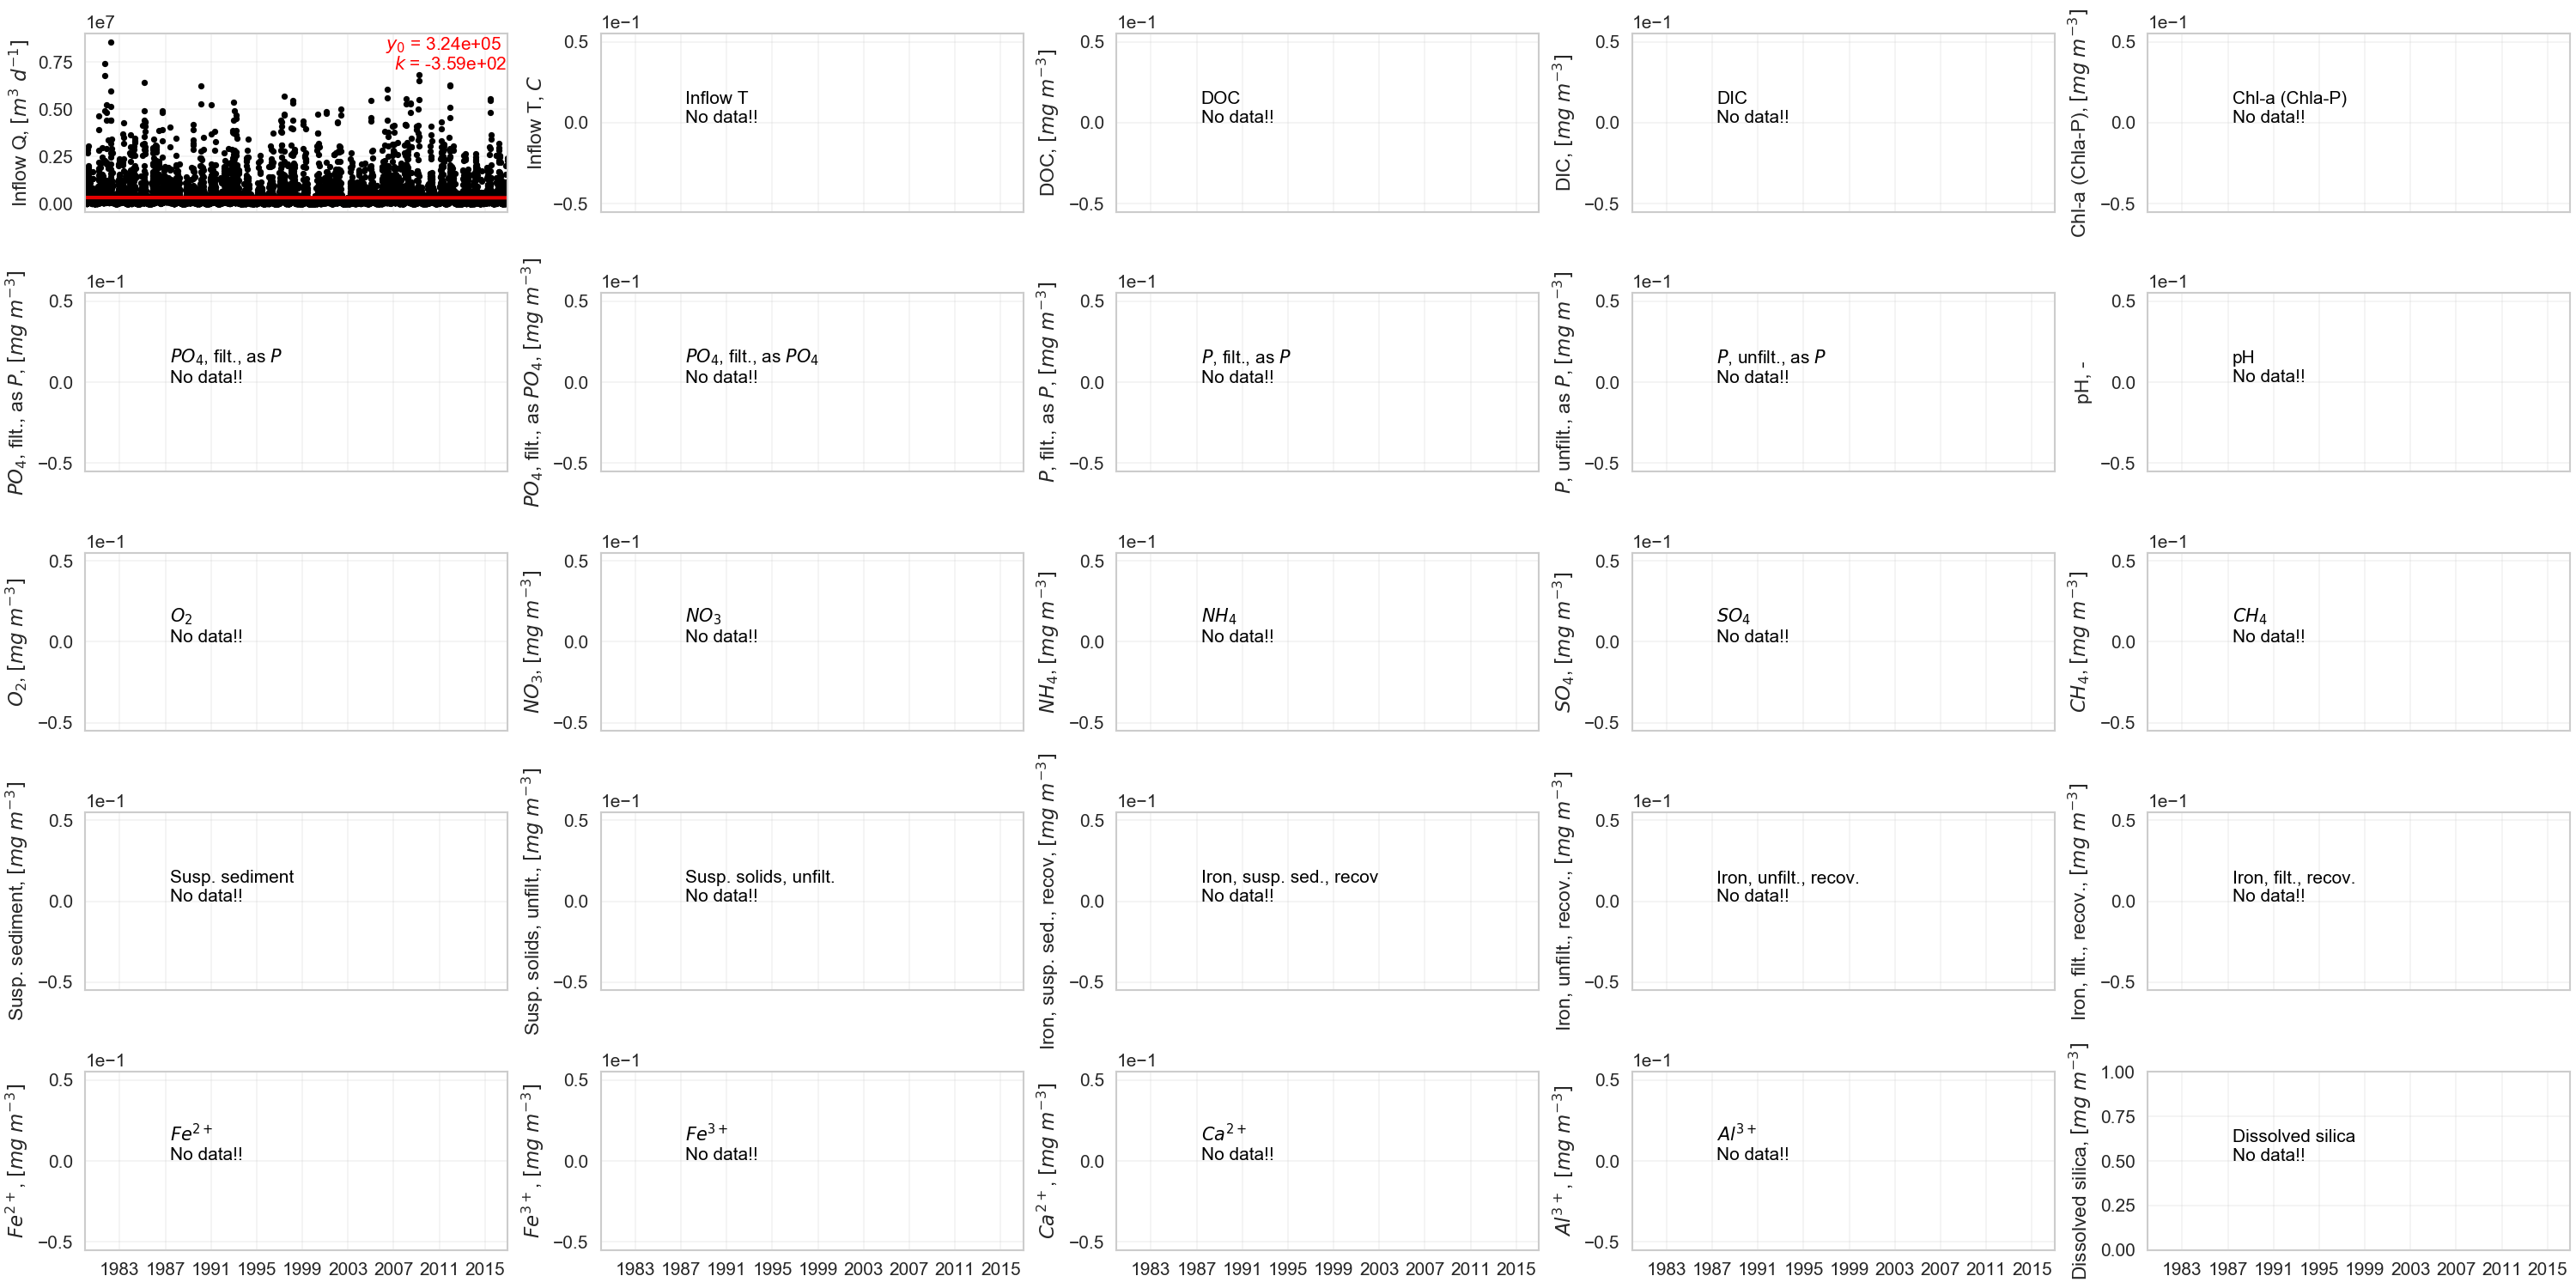
\includegraphics[width=\textwidth]{rivers/Western basin/plot_all ottawariver.png}
\end{figure}
\end{frame}


\begin{frame}
\frametitle{Western Basin: Portage river}
\begin{figure}
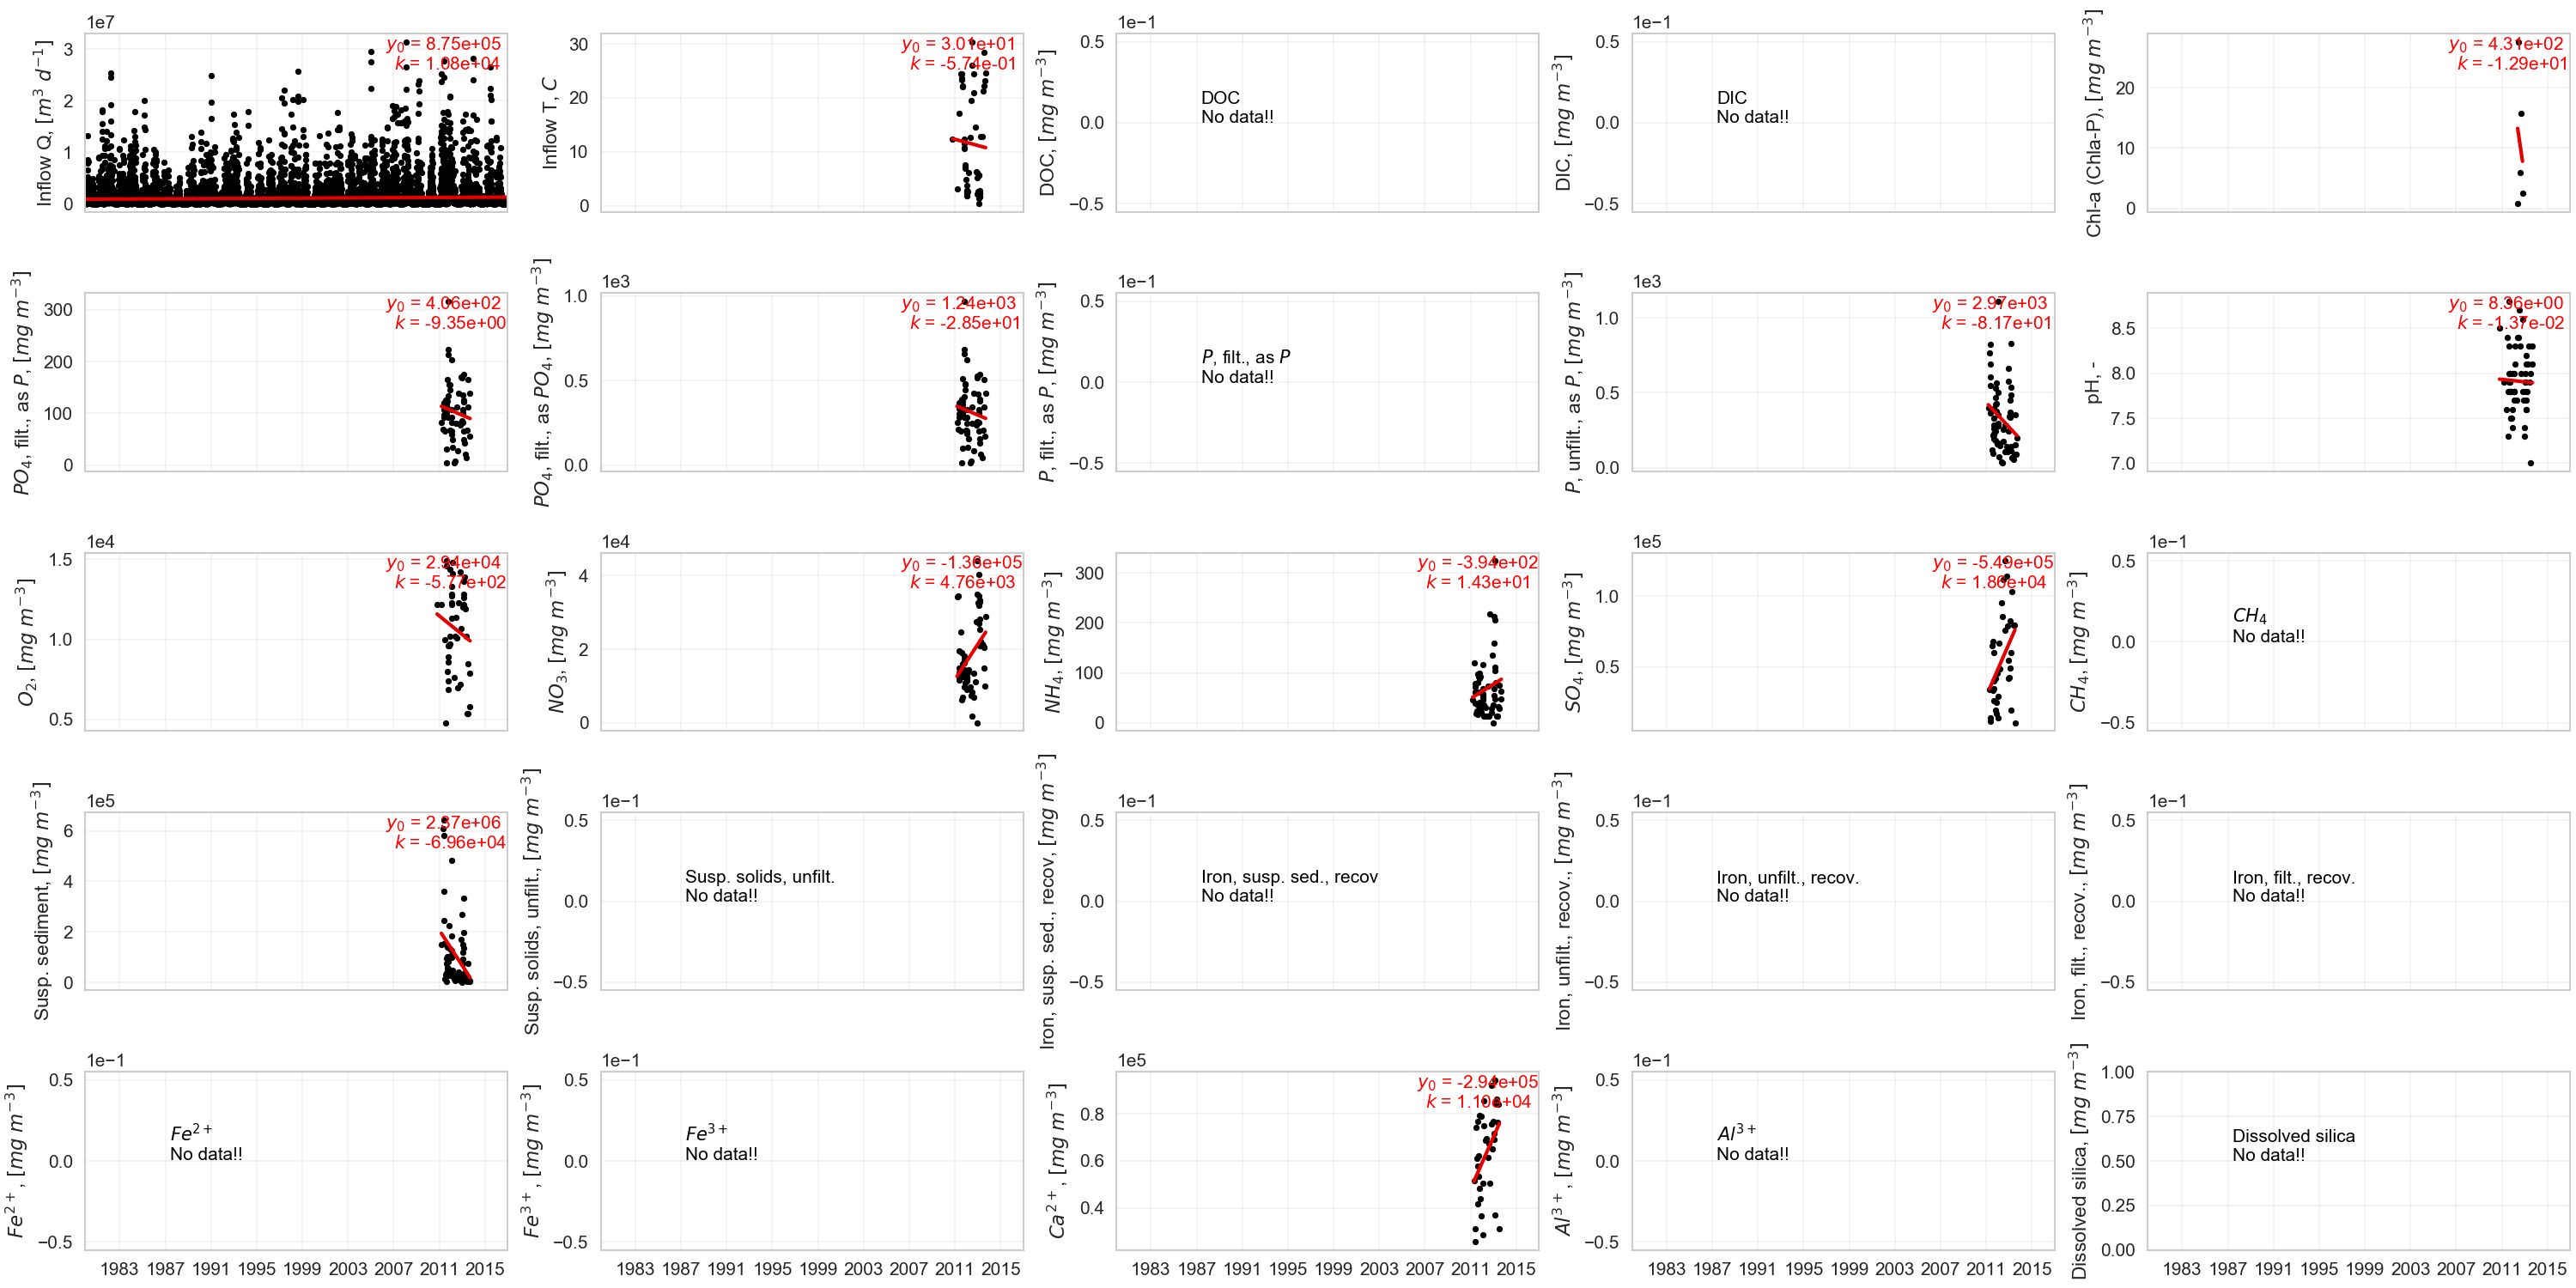
\includegraphics[width=\textwidth]{rivers/Western basin/plot_all portageriver.png}
\end{figure}
\end{frame}


\begin{frame}
\frametitle{Western Basin: Raisin river}
\begin{figure}
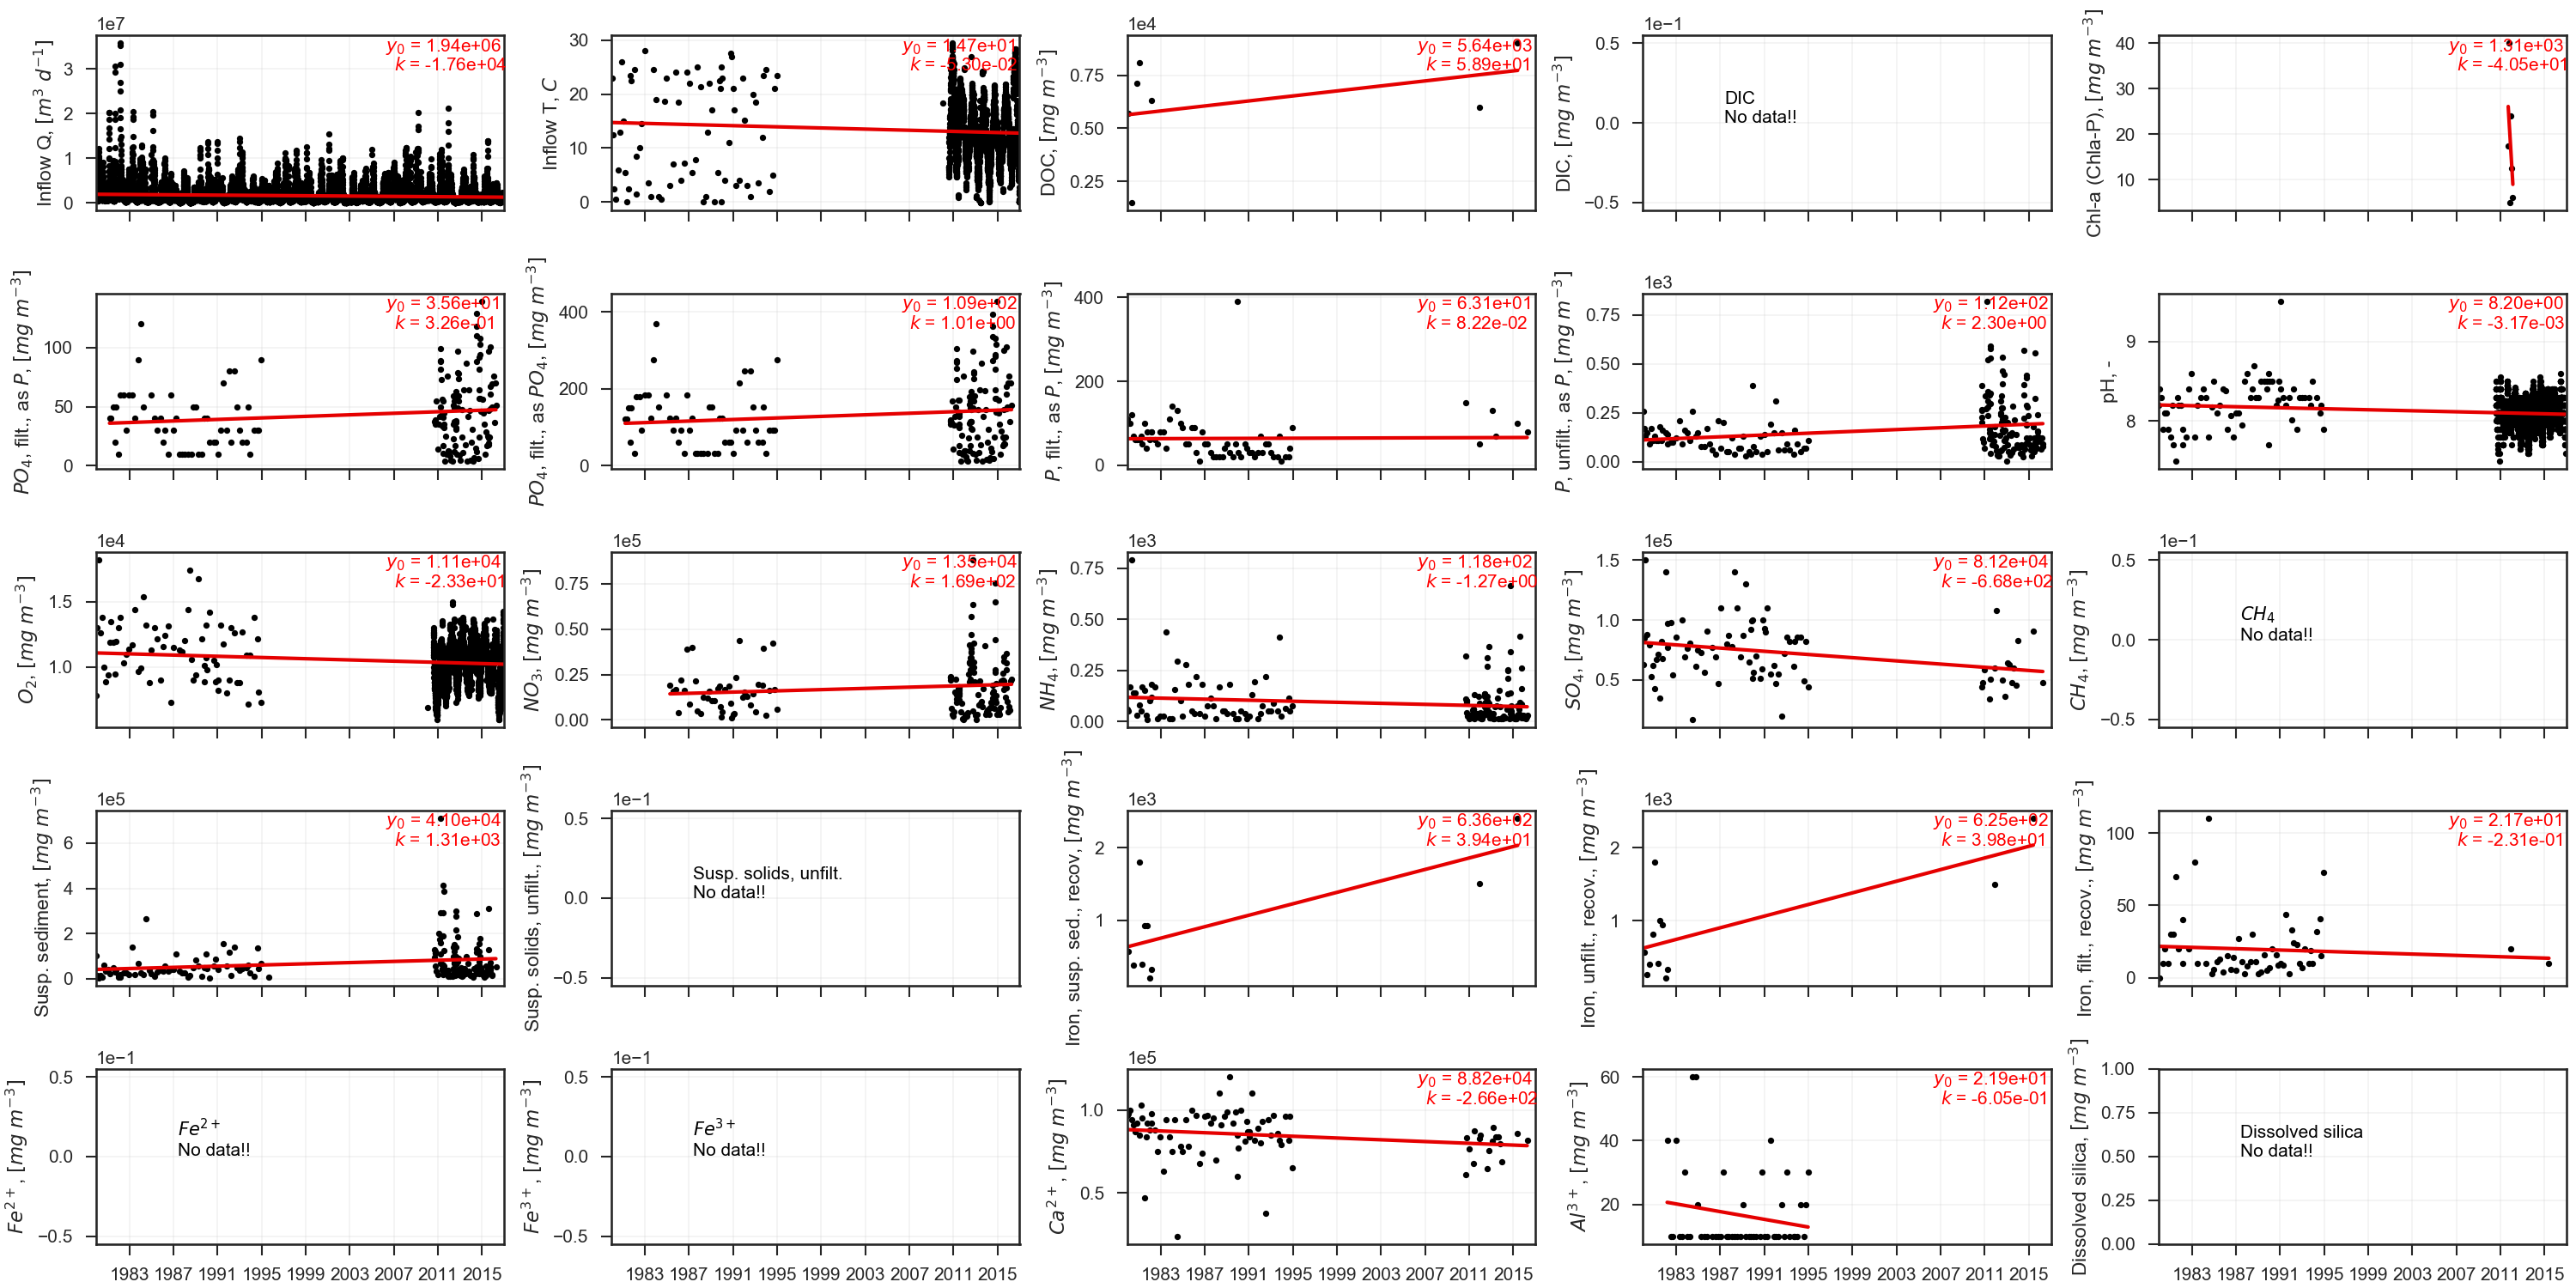
\includegraphics[width=\textwidth]{rivers/Western basin/plot_all riverraisin.png}
\end{figure}
\end{frame}


\begin{frame}
\frametitle{Western Basin: Stony creek}
\begin{figure}
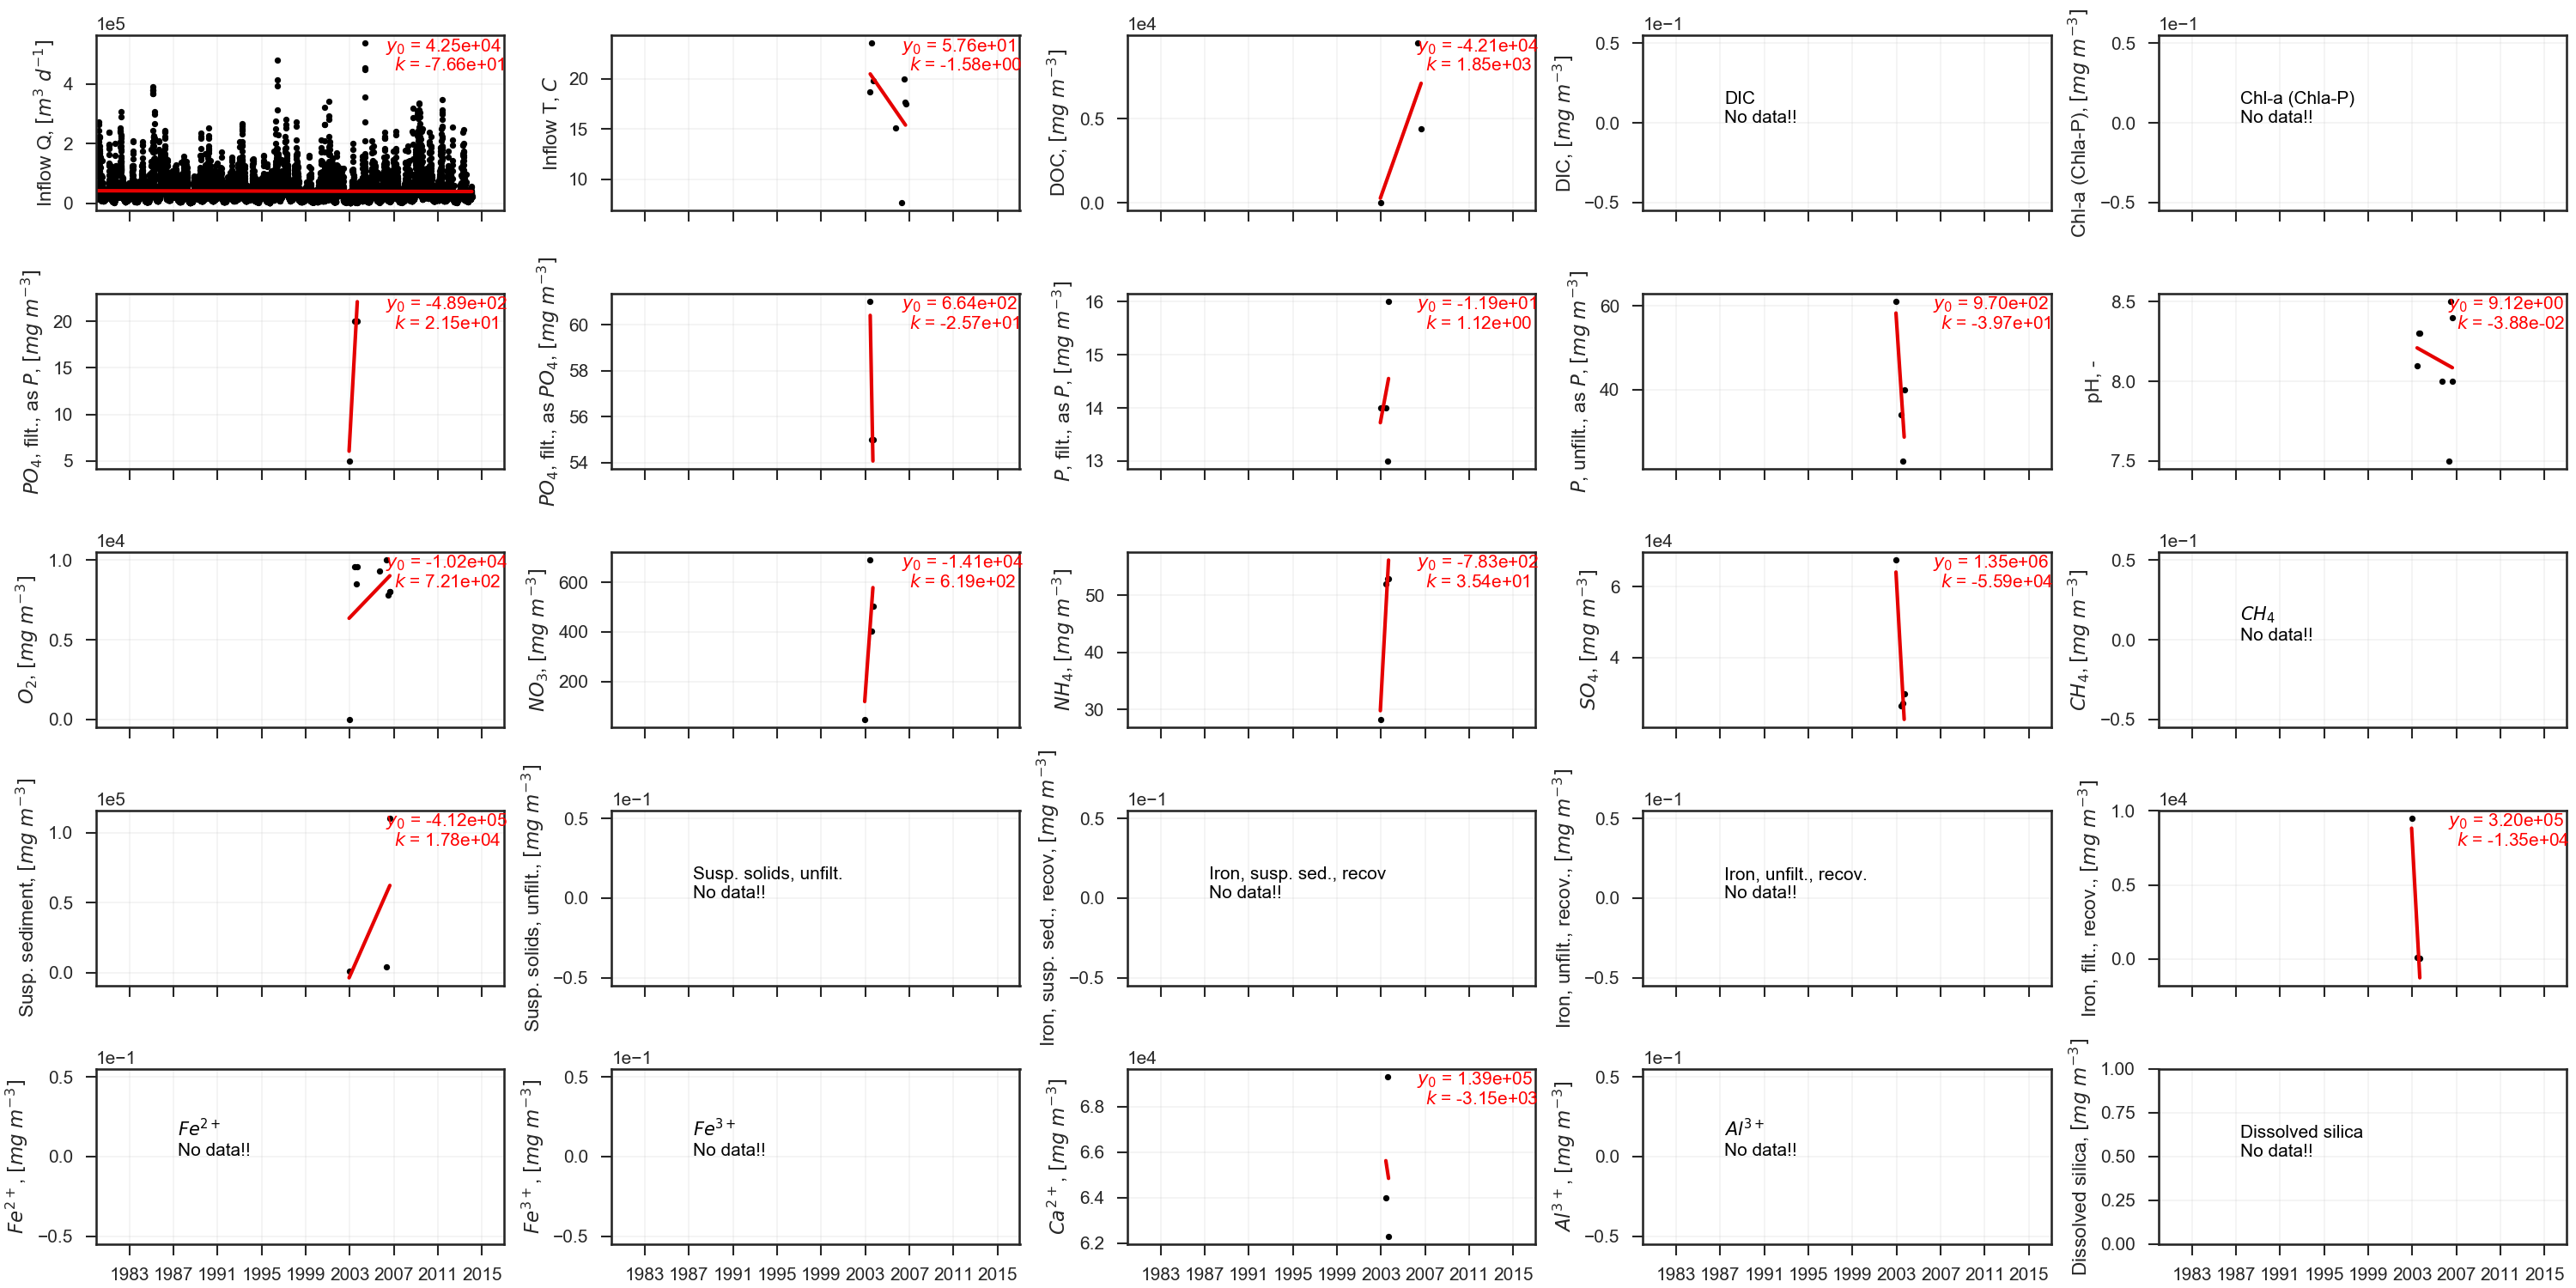
\includegraphics[width=\textwidth]{rivers/Western basin/plot_all stonycreek.png}
\end{figure}
\end{frame}


\begin{frame}
\frametitle{Western Basin: Swan creek}
\begin{figure}
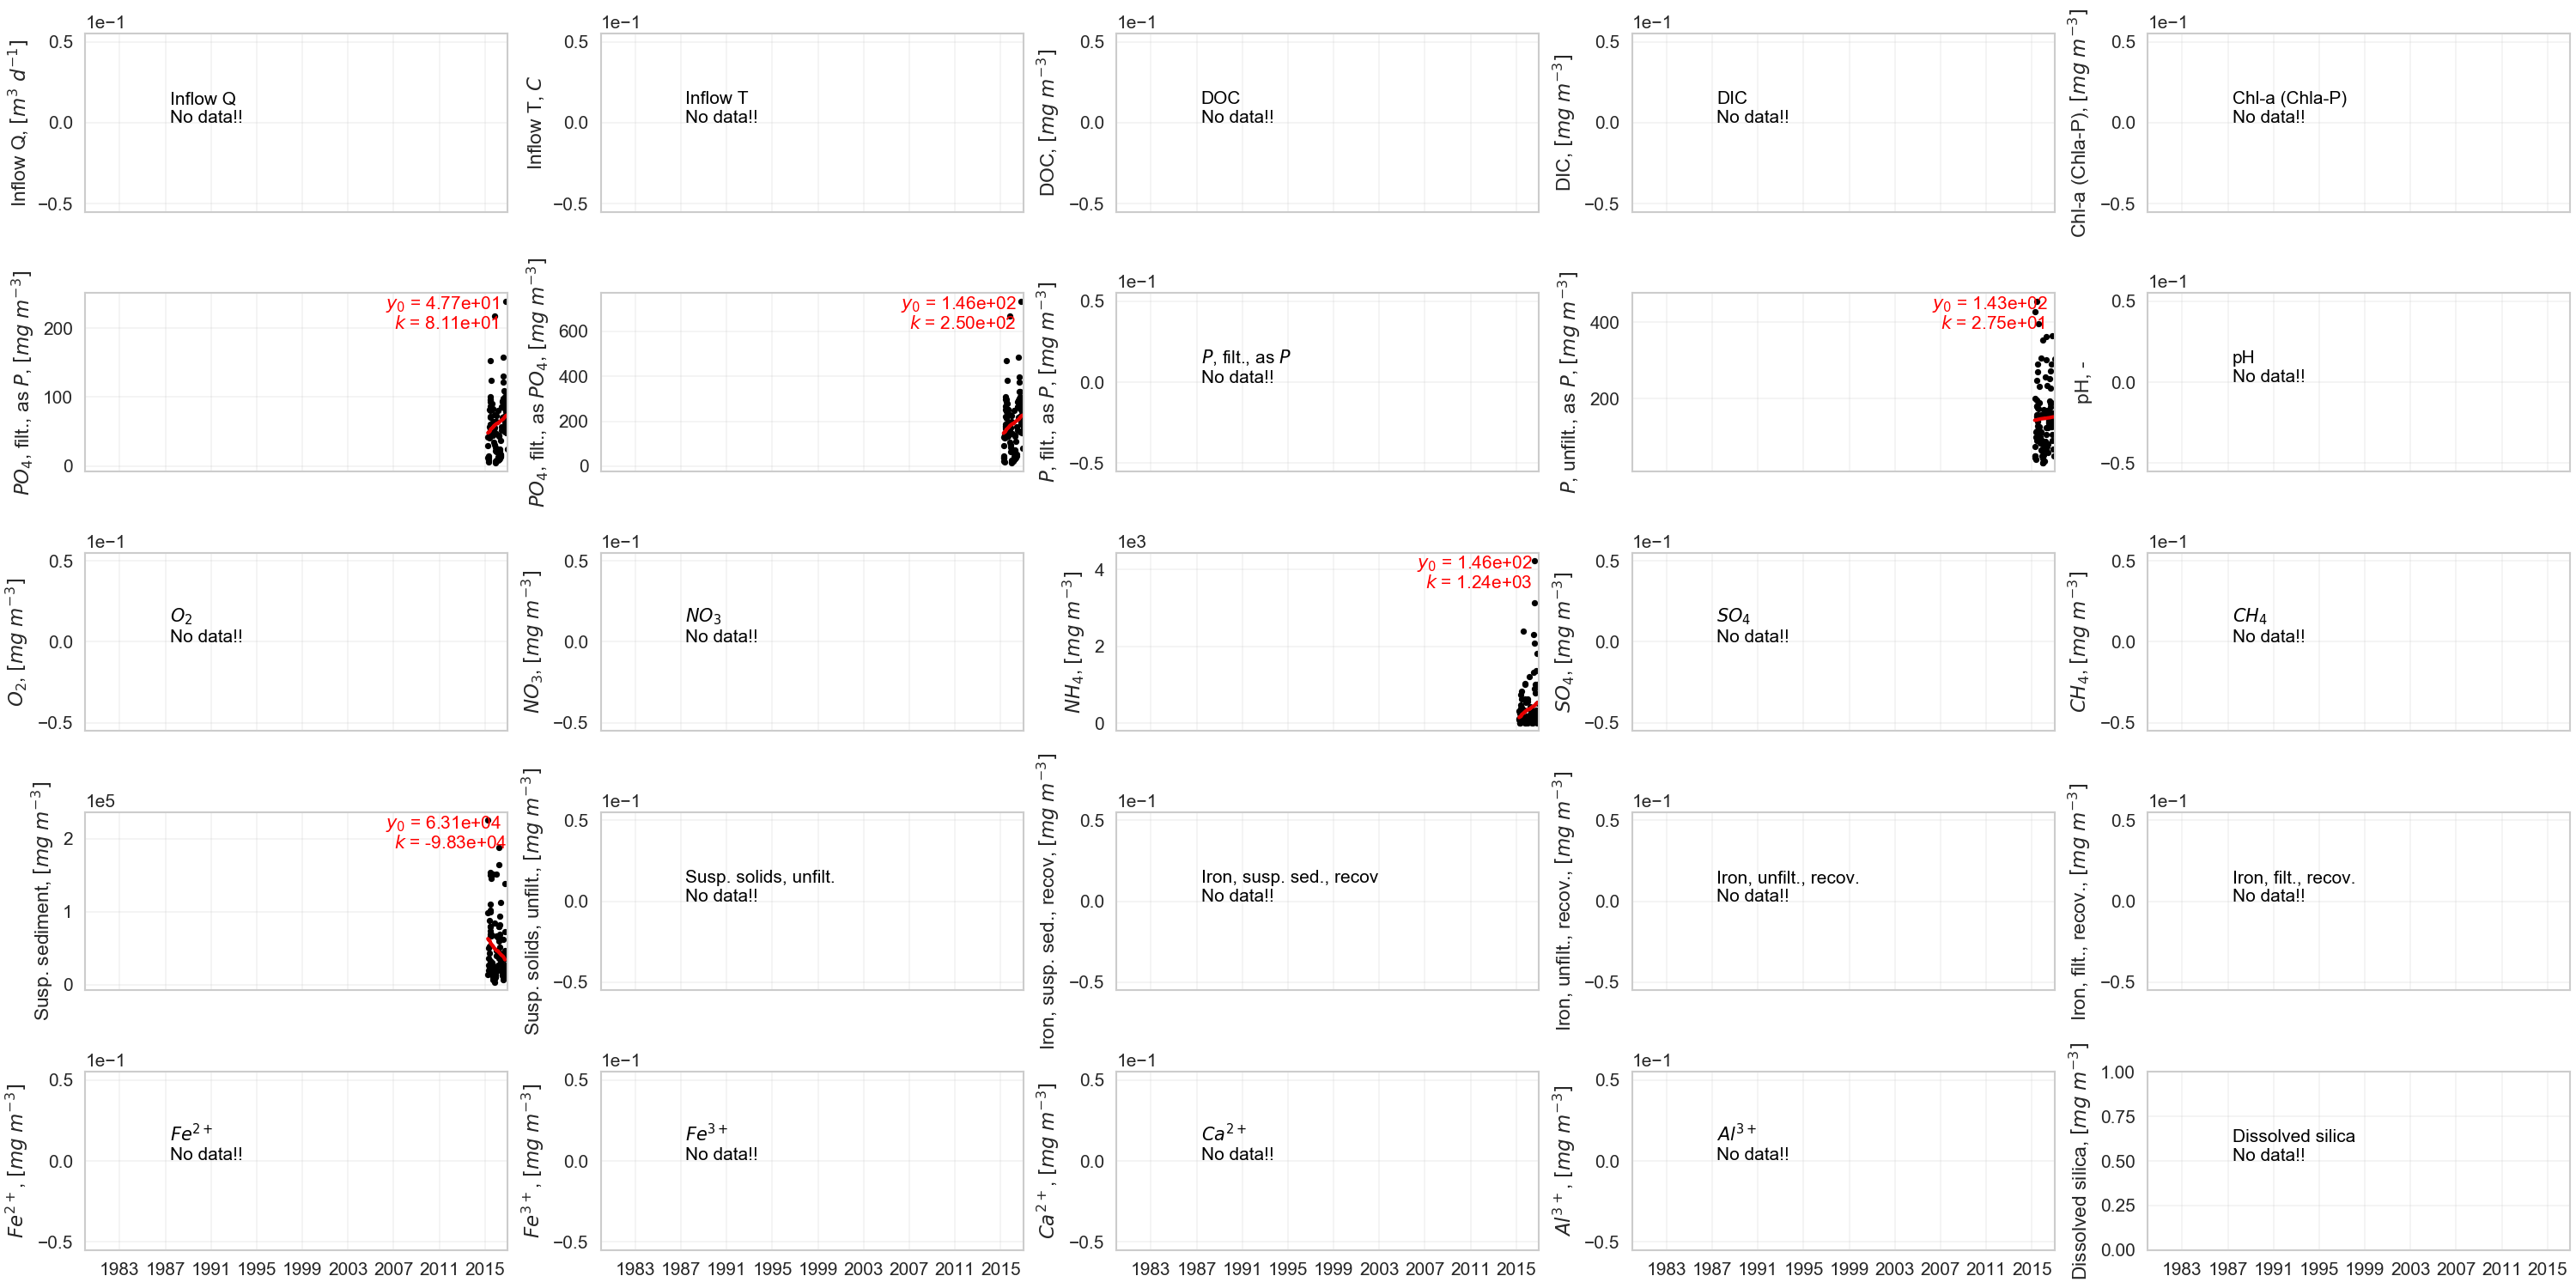
\includegraphics[width=\textwidth]{rivers/Western basin/plot_all swancreek.png}
\end{figure}
\end{frame}



\subsection{Central Basin}
\label{sub:central_basin}


\begin{frame}
\frametitle{Central Basin: Ashtabula river}
\begin{figure}
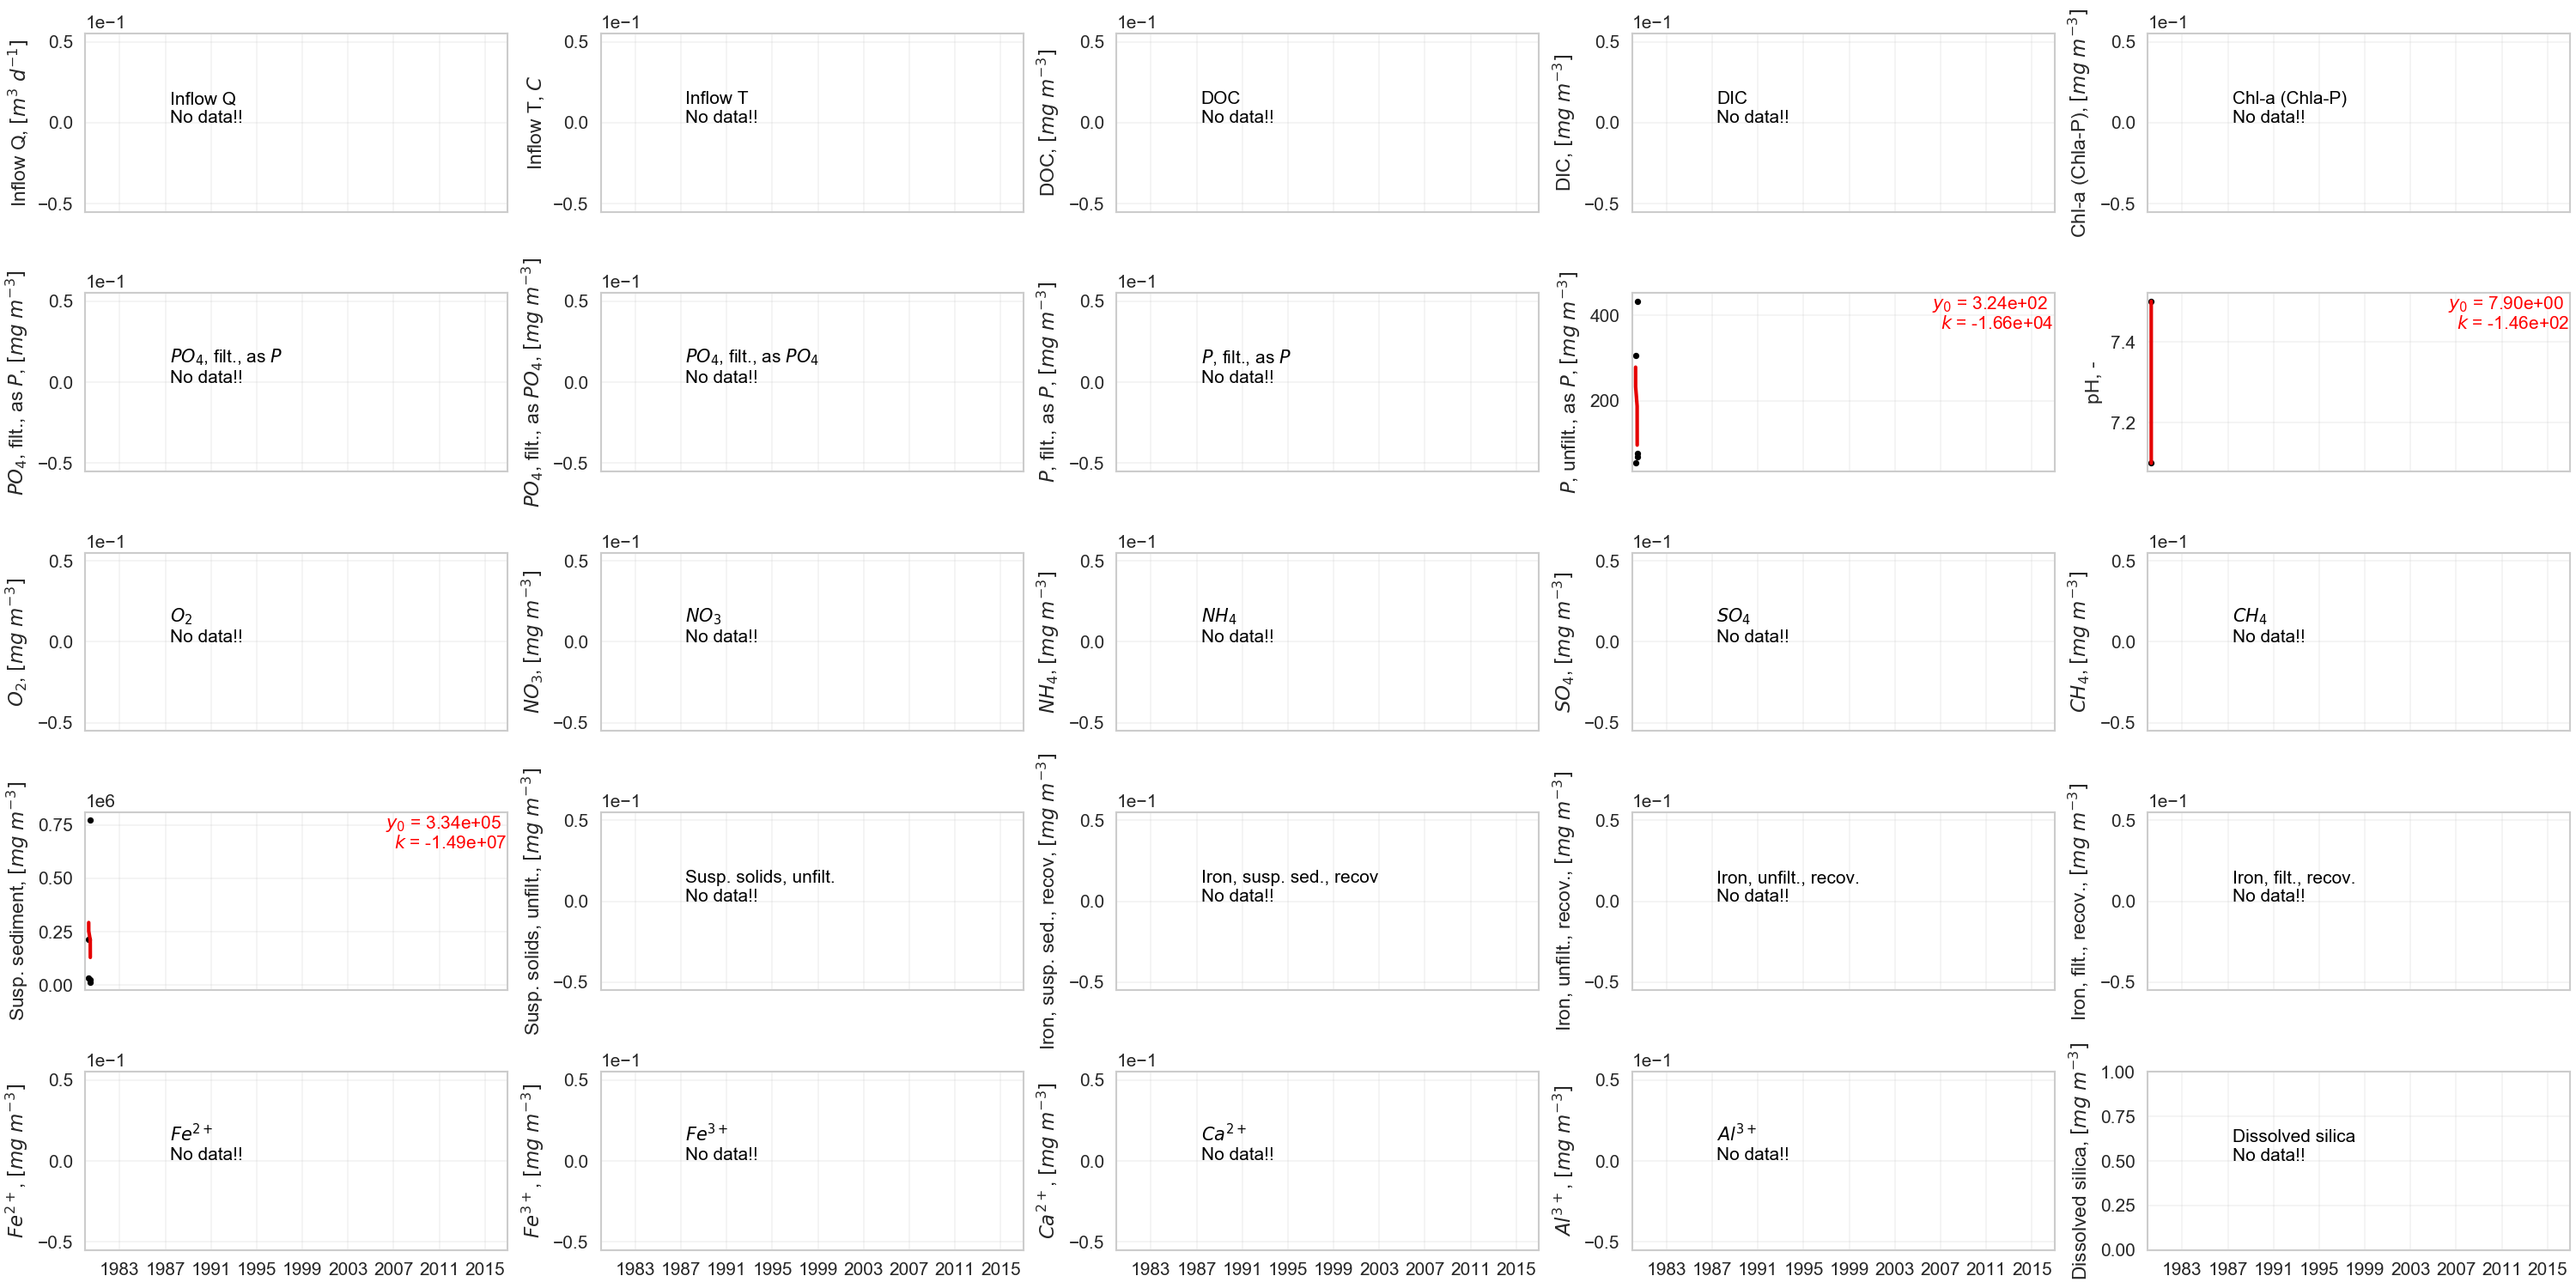
\includegraphics[width=\textwidth]{rivers/Central basin/plot_all ashtabulariver.png}
\end{figure}
\end{frame}

\begin{frame}
\frametitle{Central Basin: Black river}
\begin{figure}
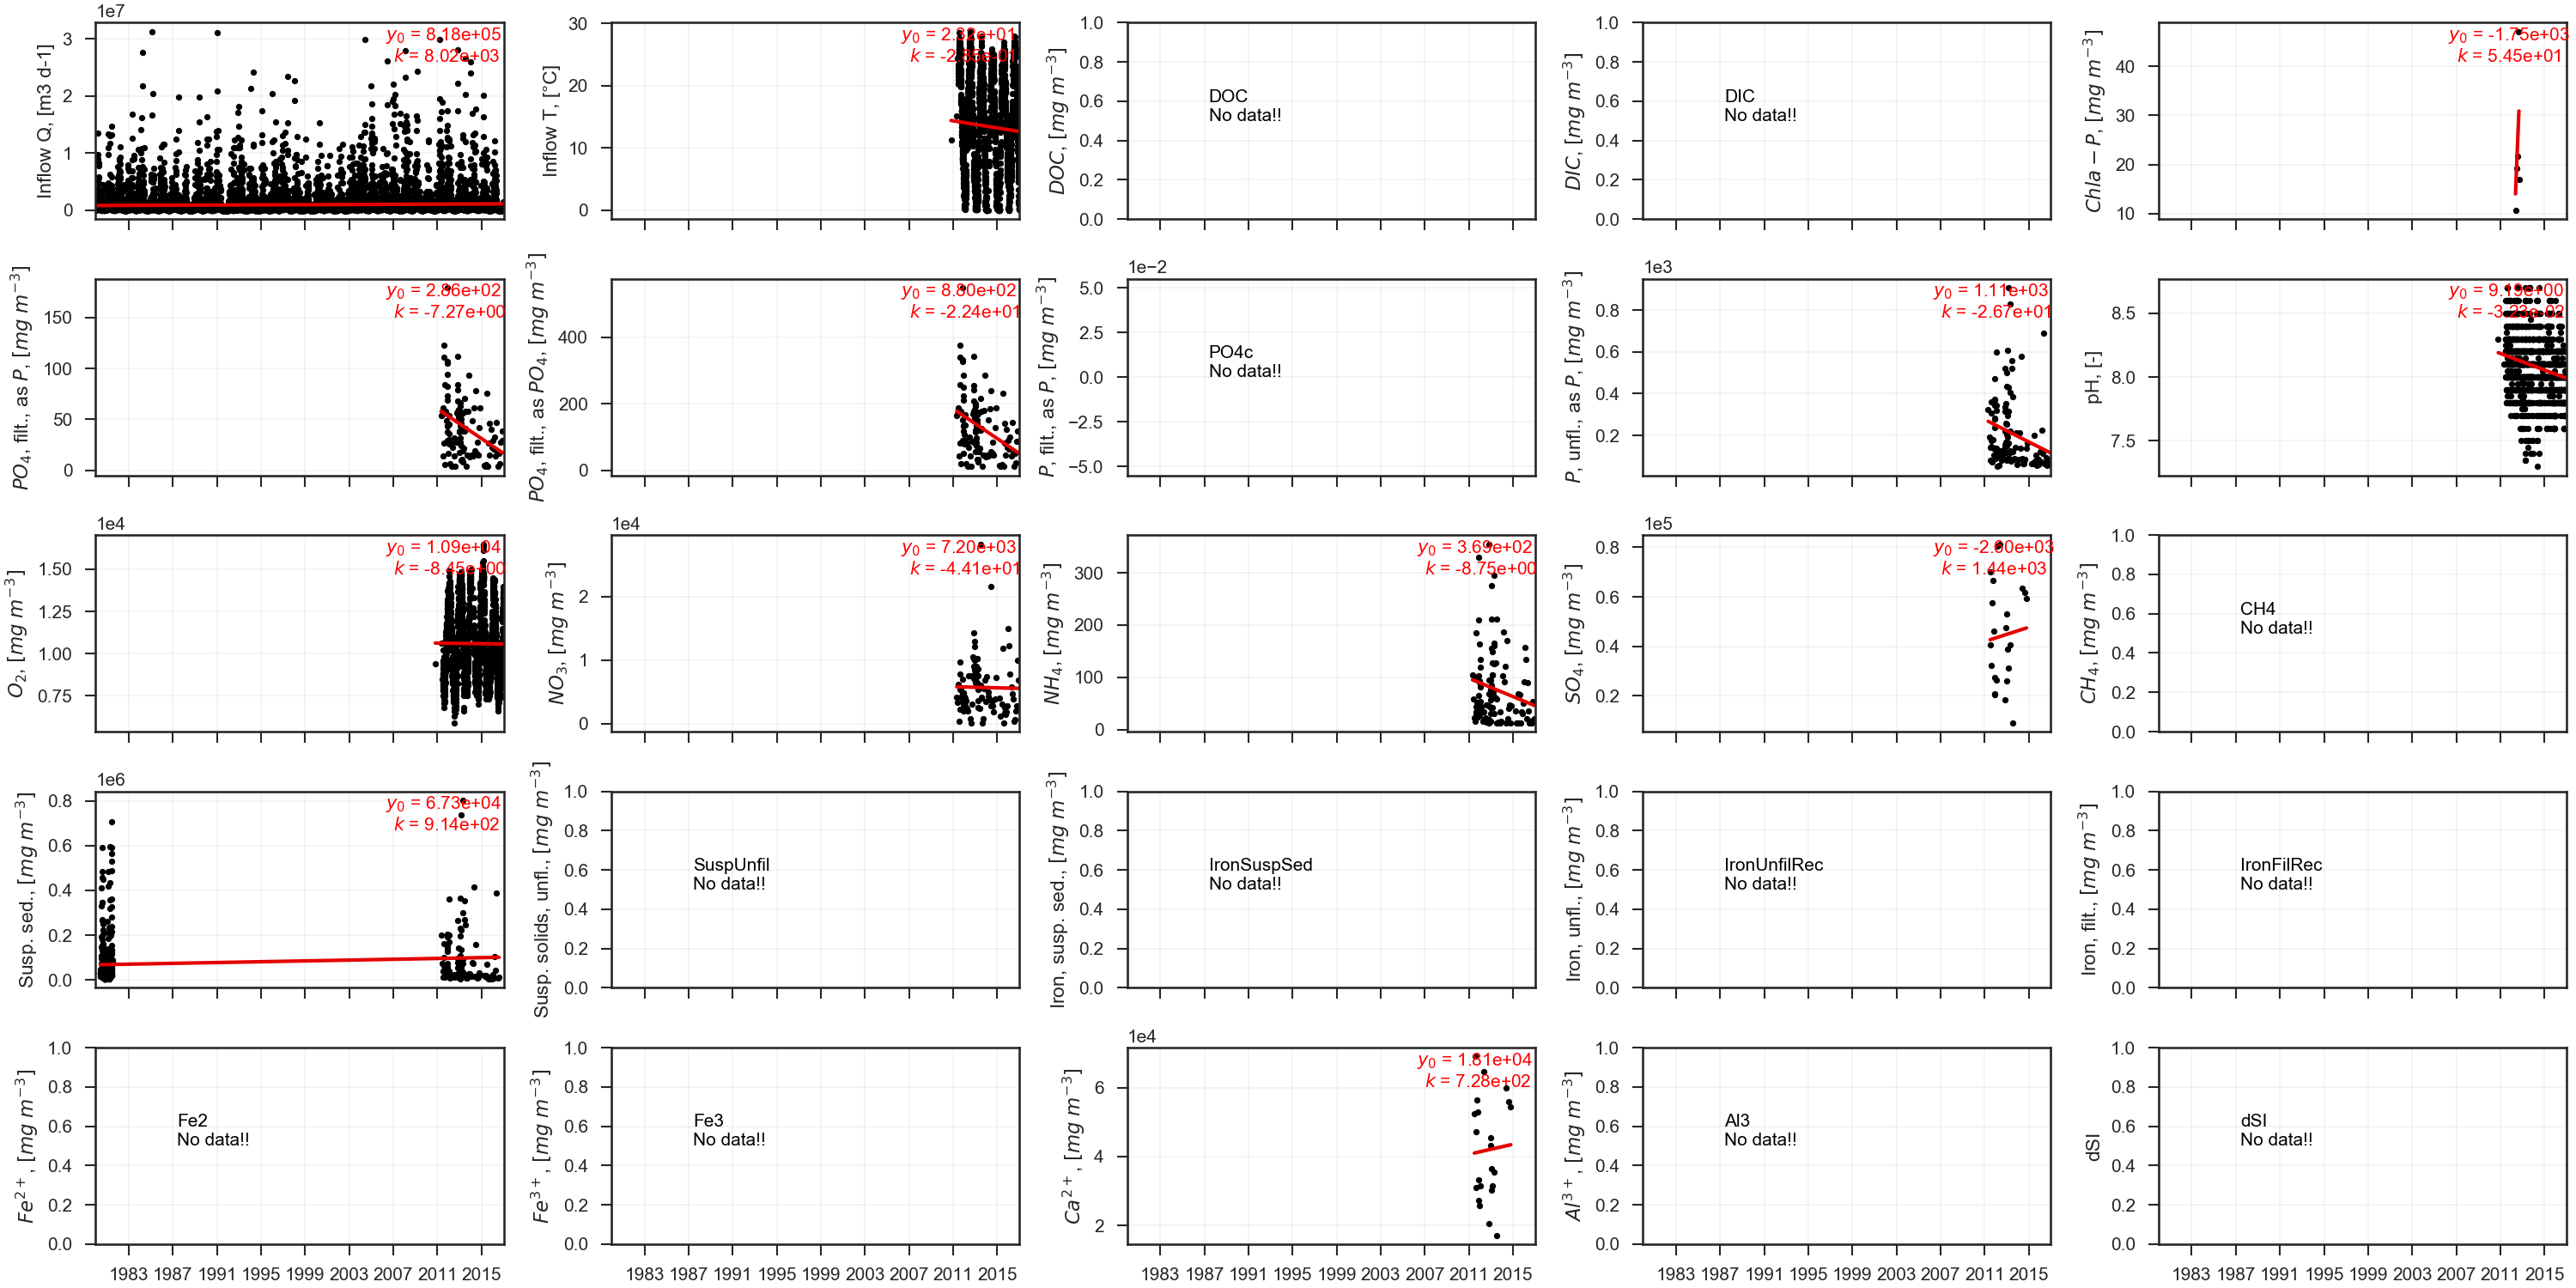
\includegraphics[width=\textwidth]{rivers/Central basin/plot_all blackriver.png}
\end{figure}
\end{frame}

\begin{frame}
\frametitle{Central Basin: Chagrin river}
\begin{figure}
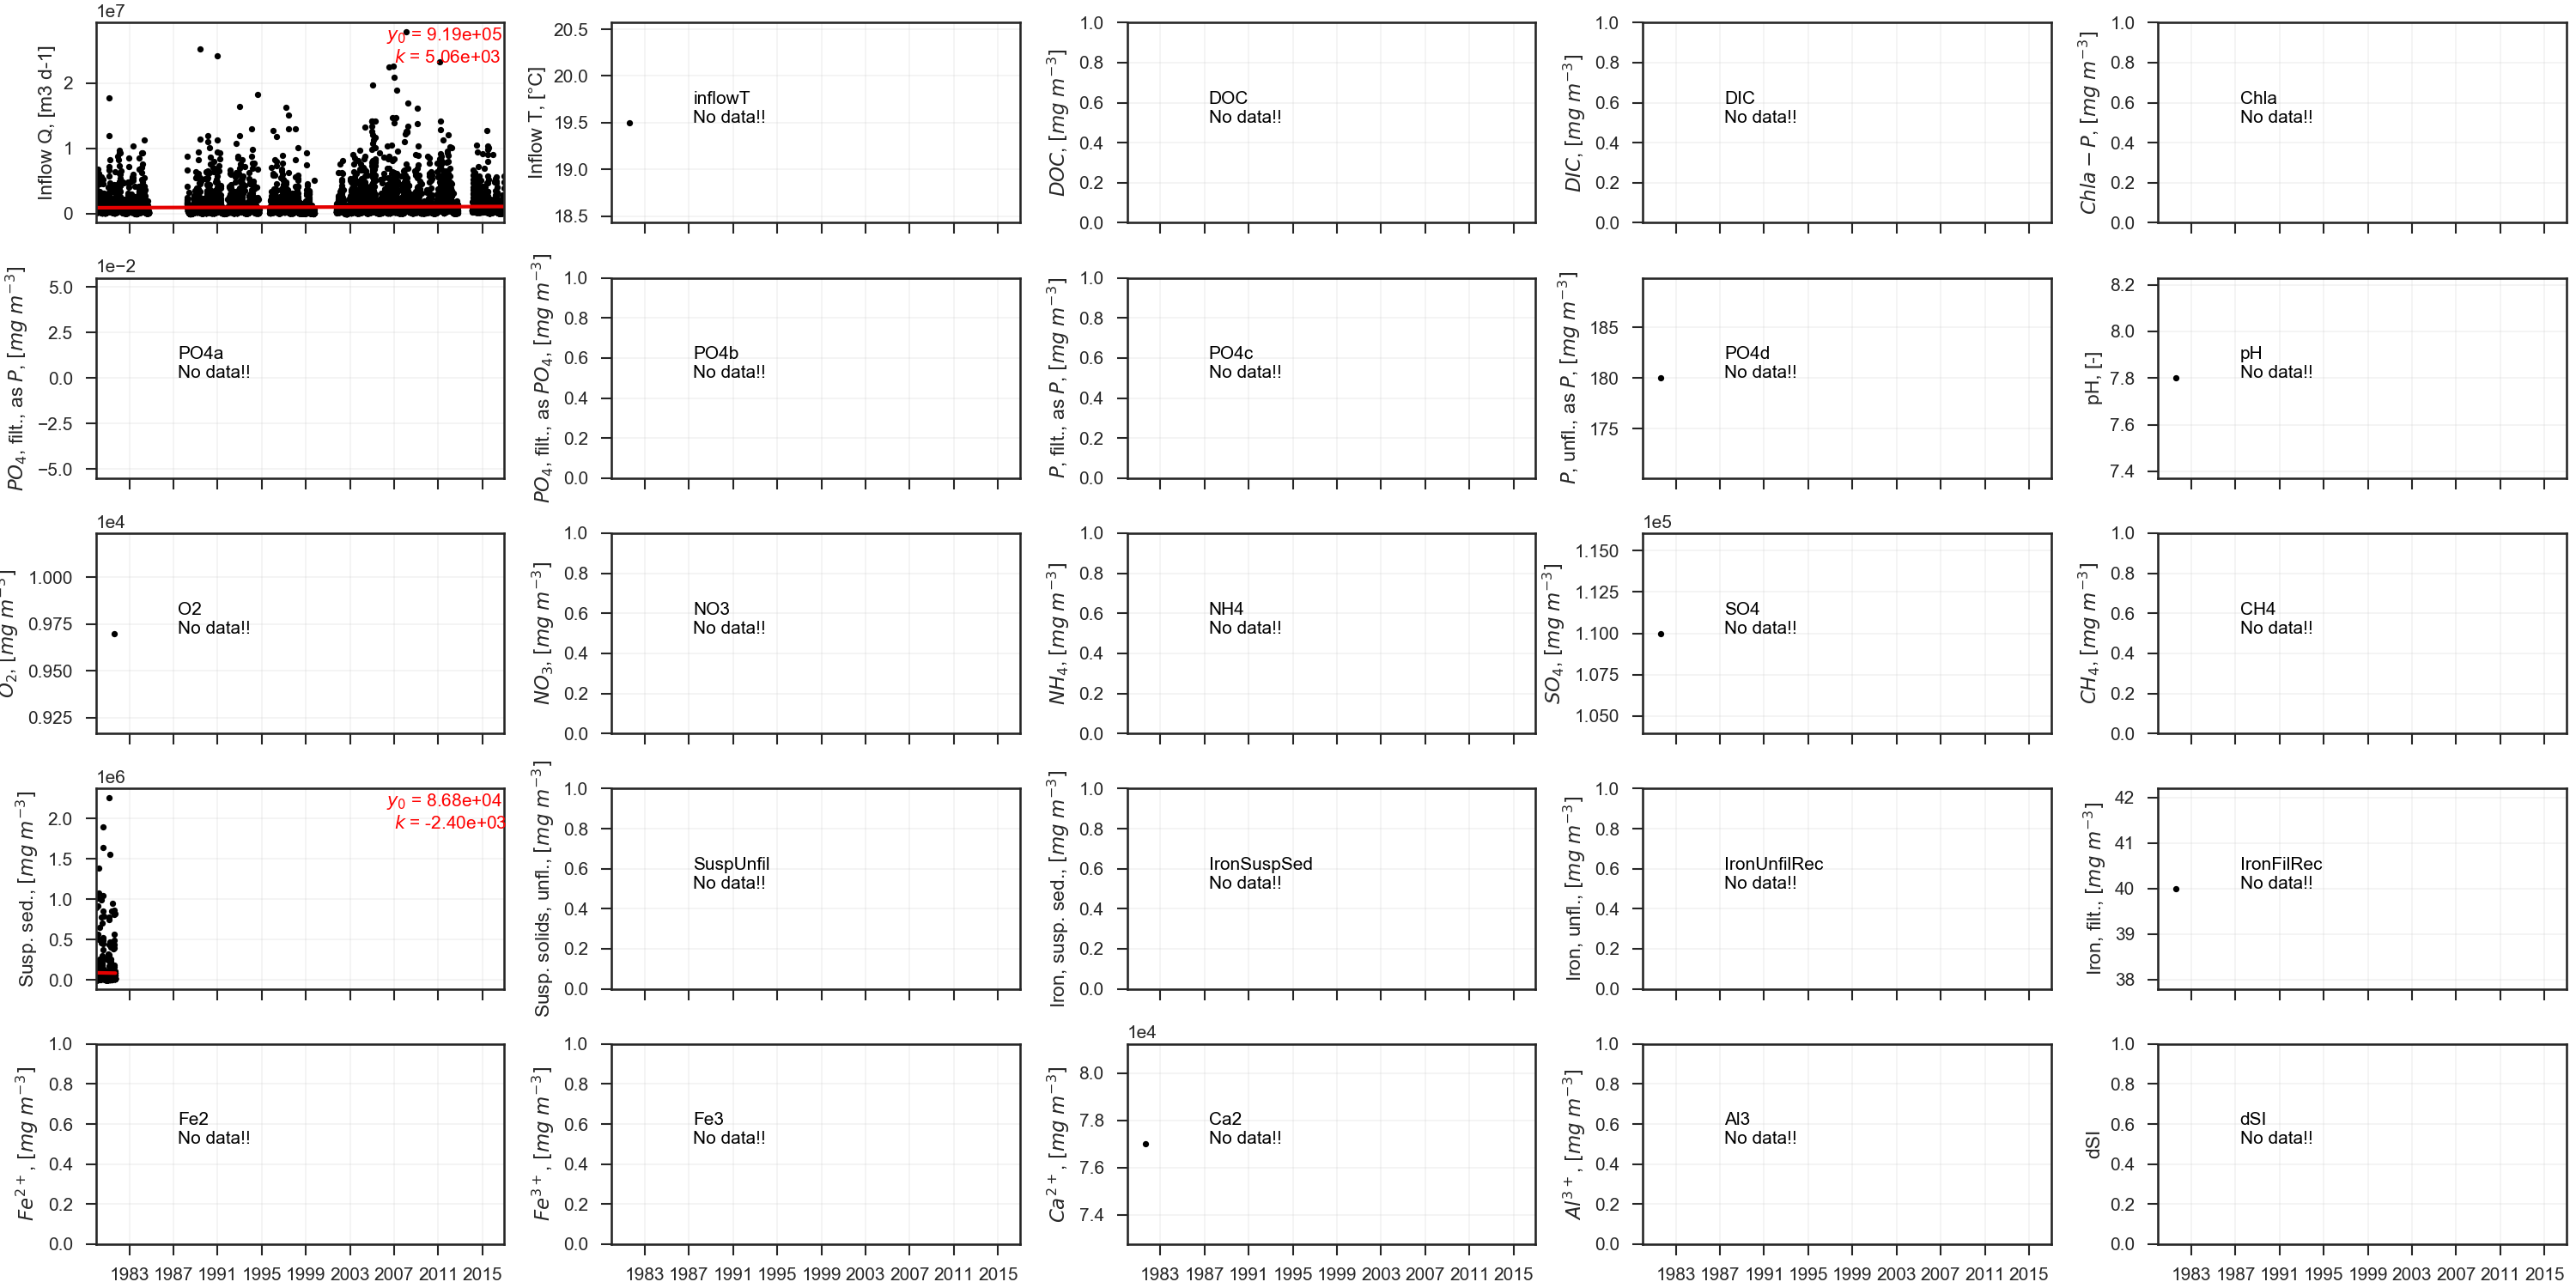
\includegraphics[width=\textwidth]{rivers/Central basin/plot_all chagrinriver.png}
\end{figure}
\end{frame}

\begin{frame}
\frametitle{Central Basin: Conneaut creek}
\begin{figure}
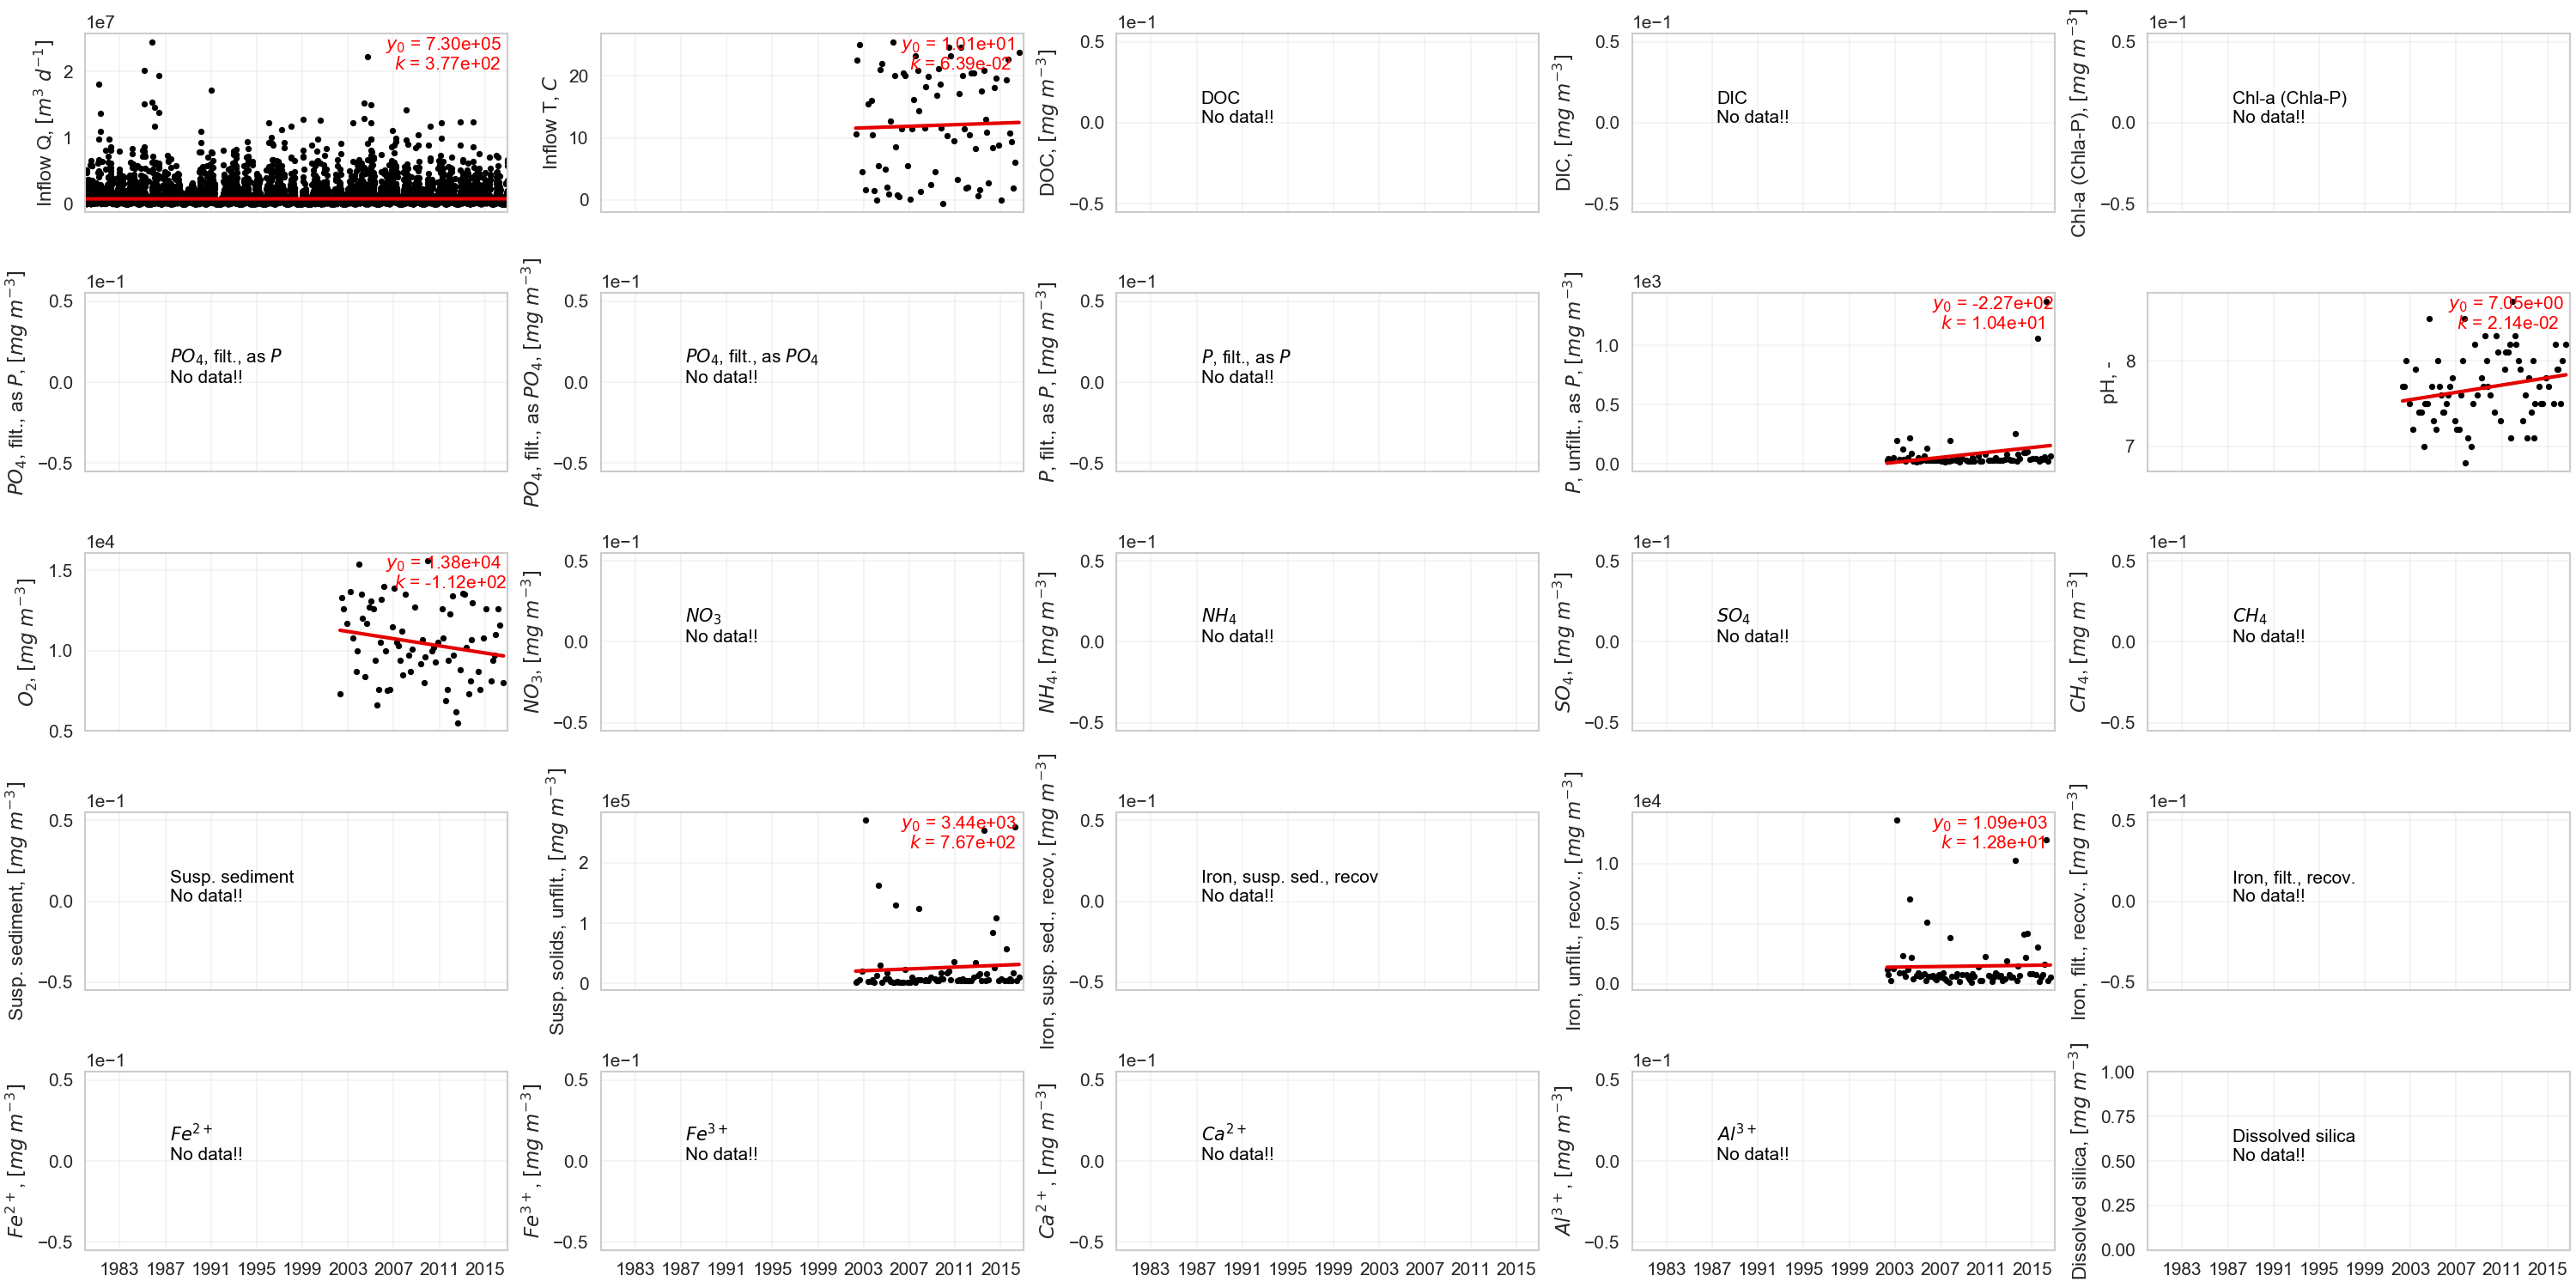
\includegraphics[width=\textwidth]{rivers/Central basin/plot_all conneautcreek.png}
\end{figure}
\end{frame}

\begin{frame}
\frametitle{Central Basin: Cuyahoga river}
\begin{figure}
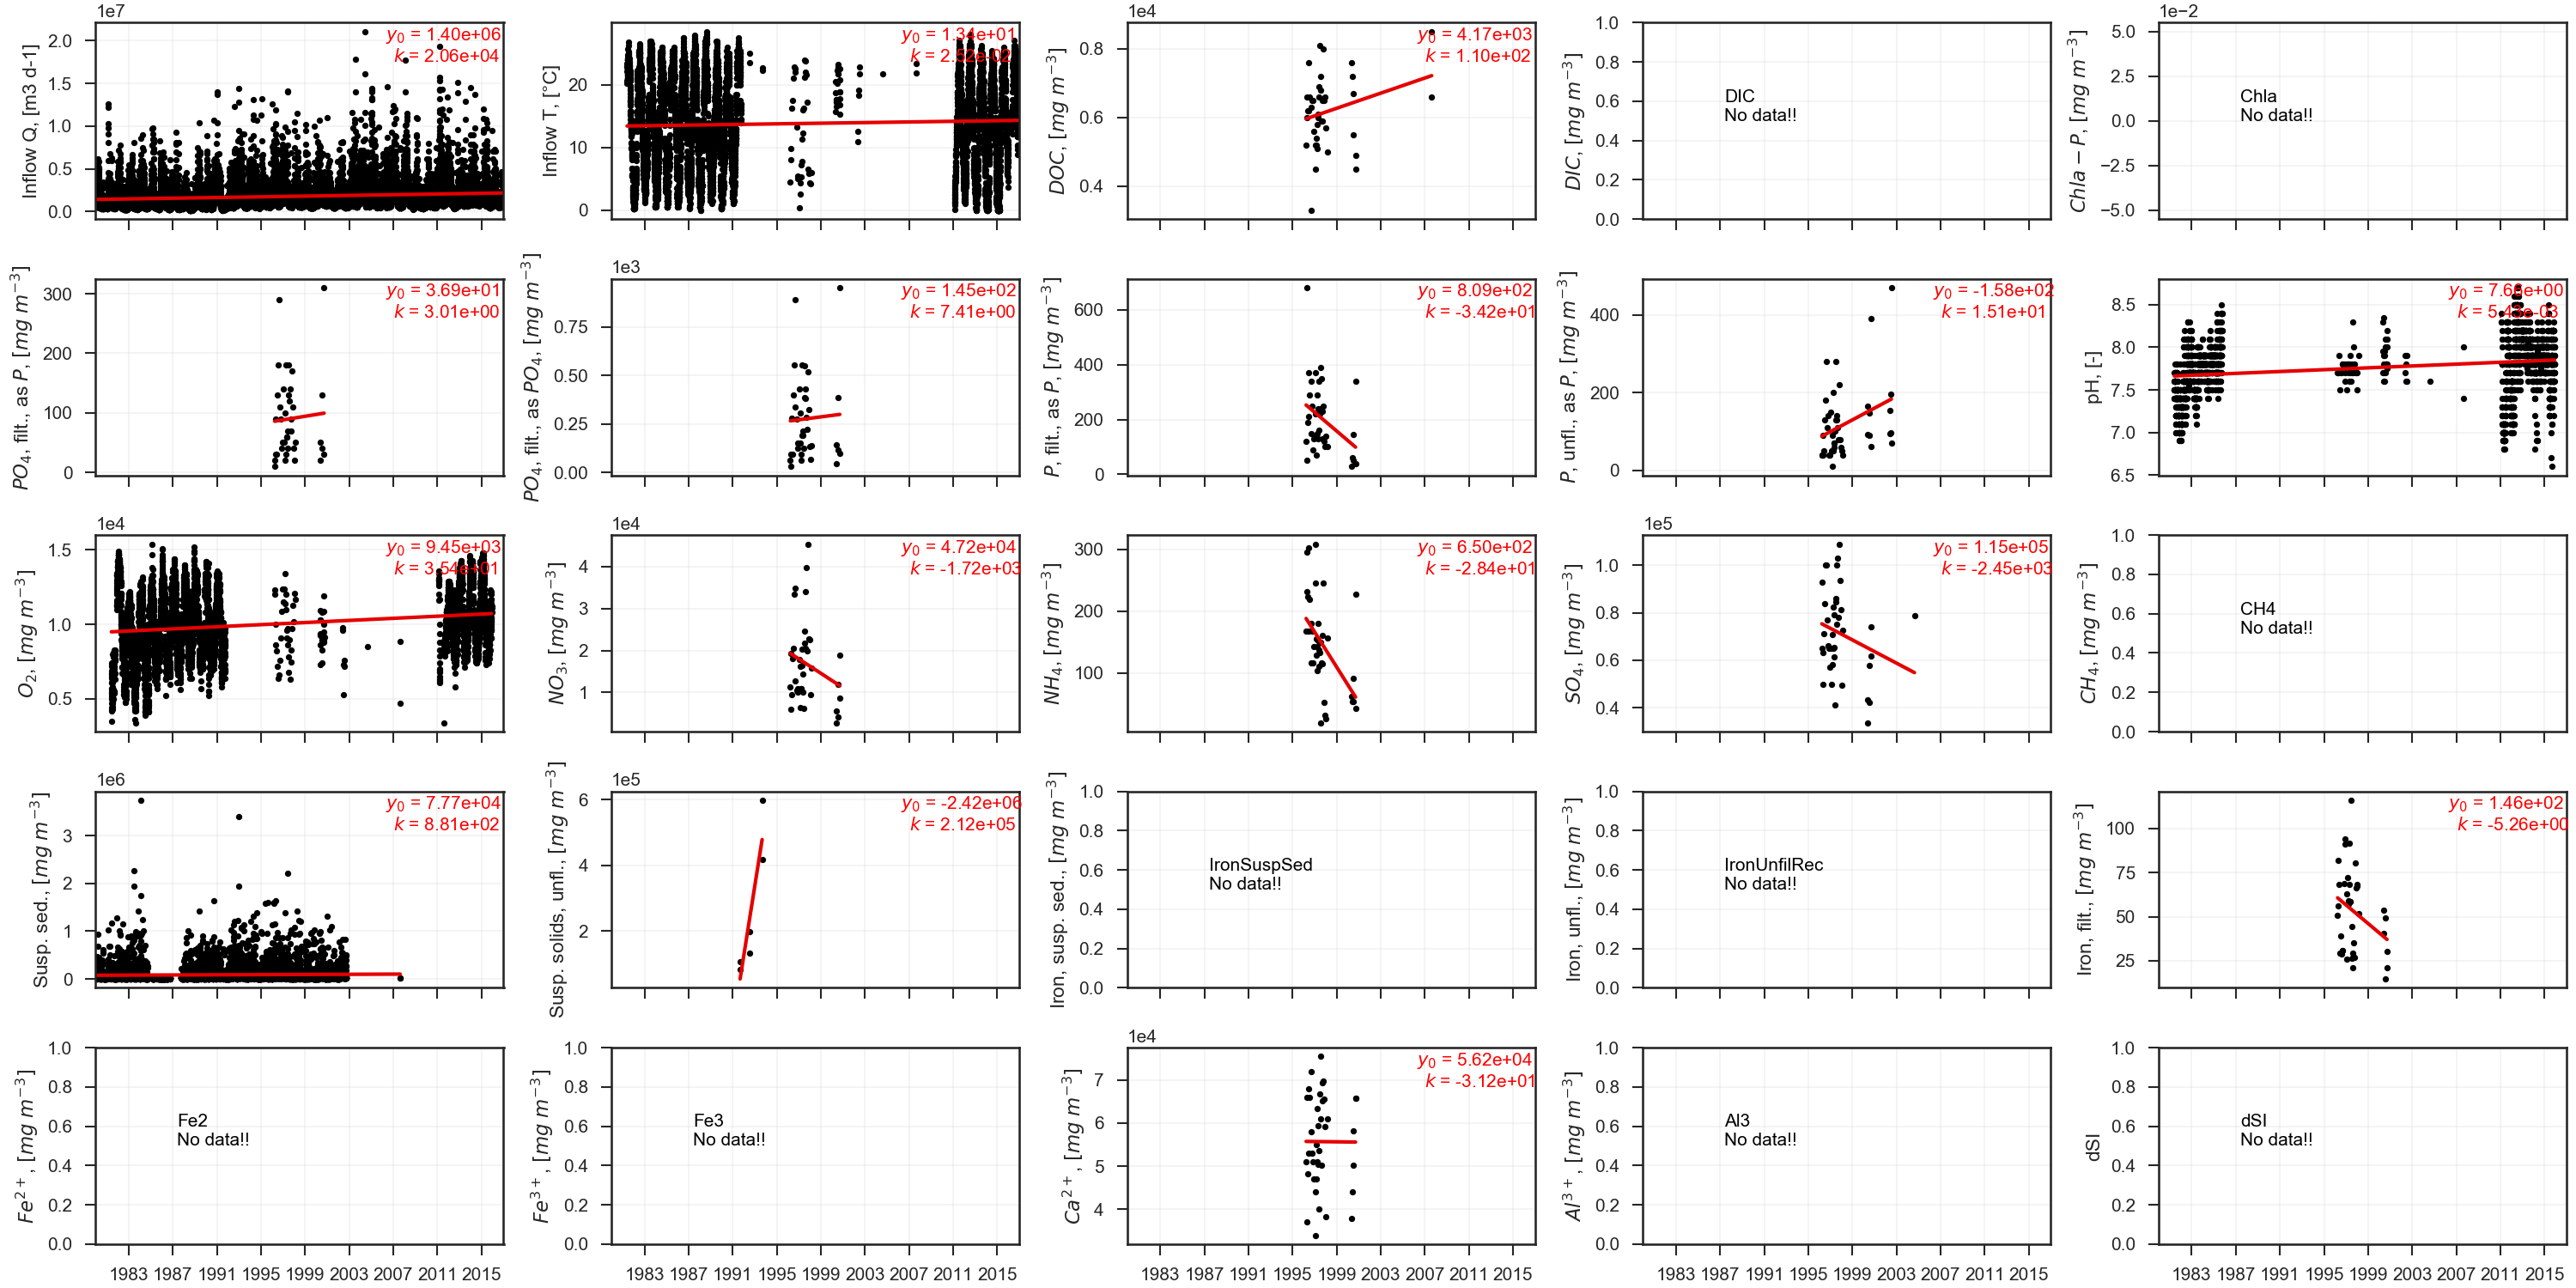
\includegraphics[width=\textwidth]{rivers/Central basin/plot_all cuyahogariver.png}
\end{figure}
\end{frame}

\begin{frame}
\frametitle{Central Basin: Grand river}
\begin{figure}
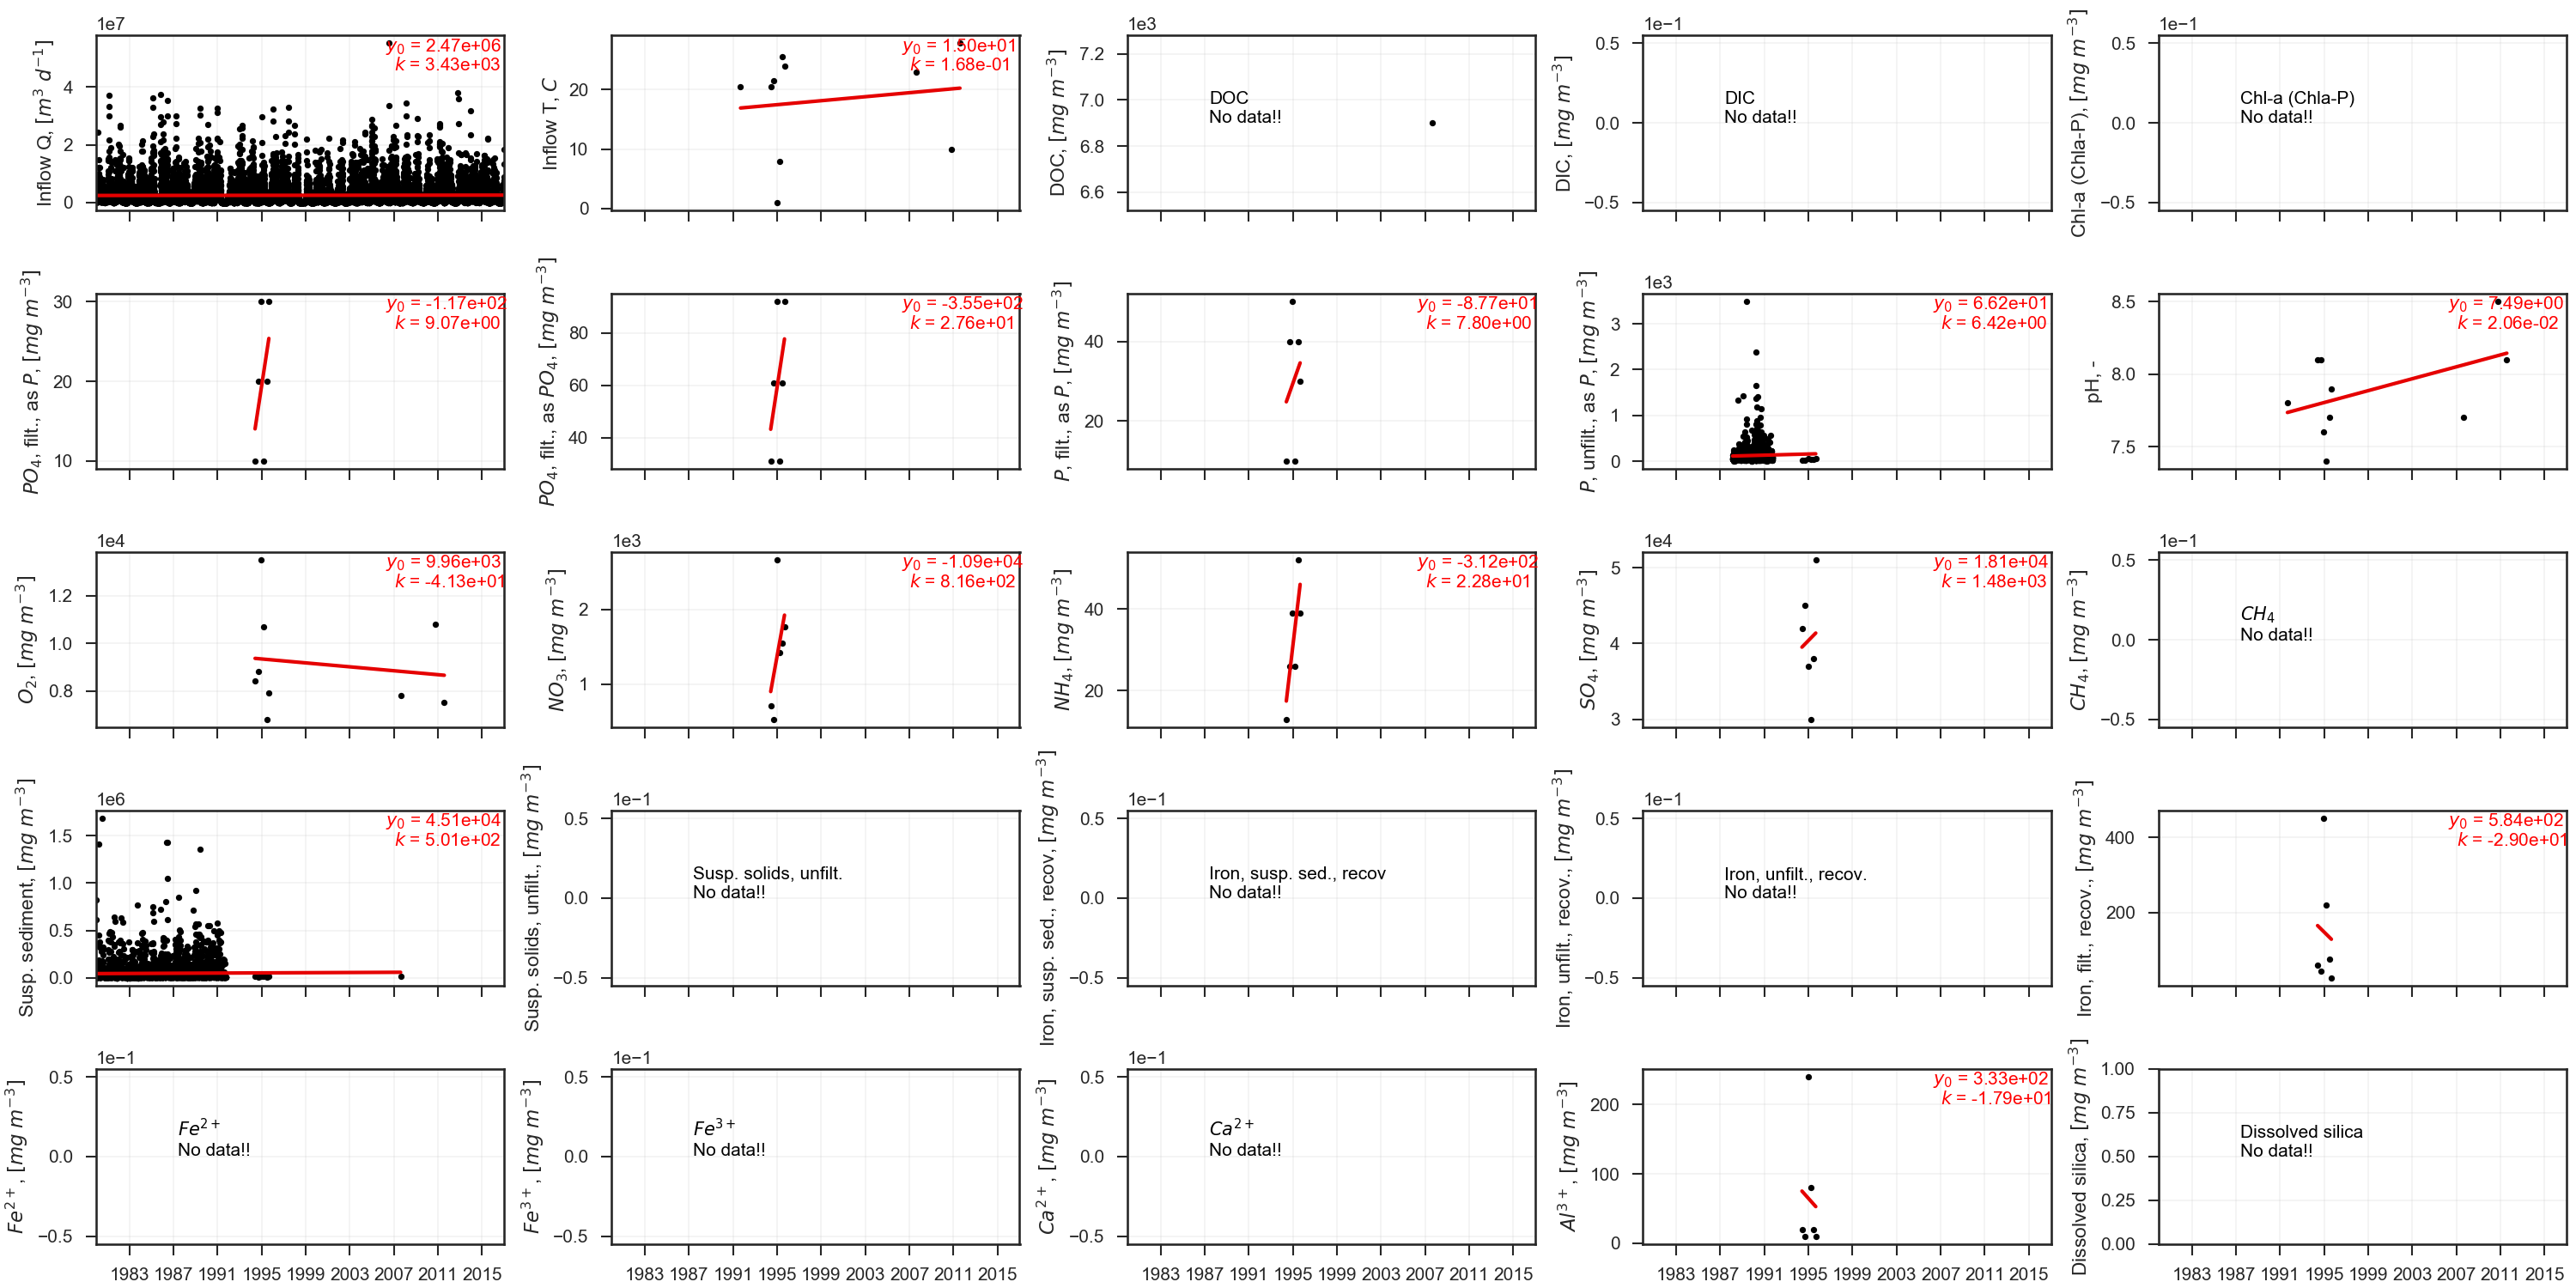
\includegraphics[width=\textwidth]{rivers/Central basin/plot_all grandriver.png}
\end{figure}
\end{frame}

\begin{frame}
\frametitle{Central Basin: Rocky river}
\begin{figure}
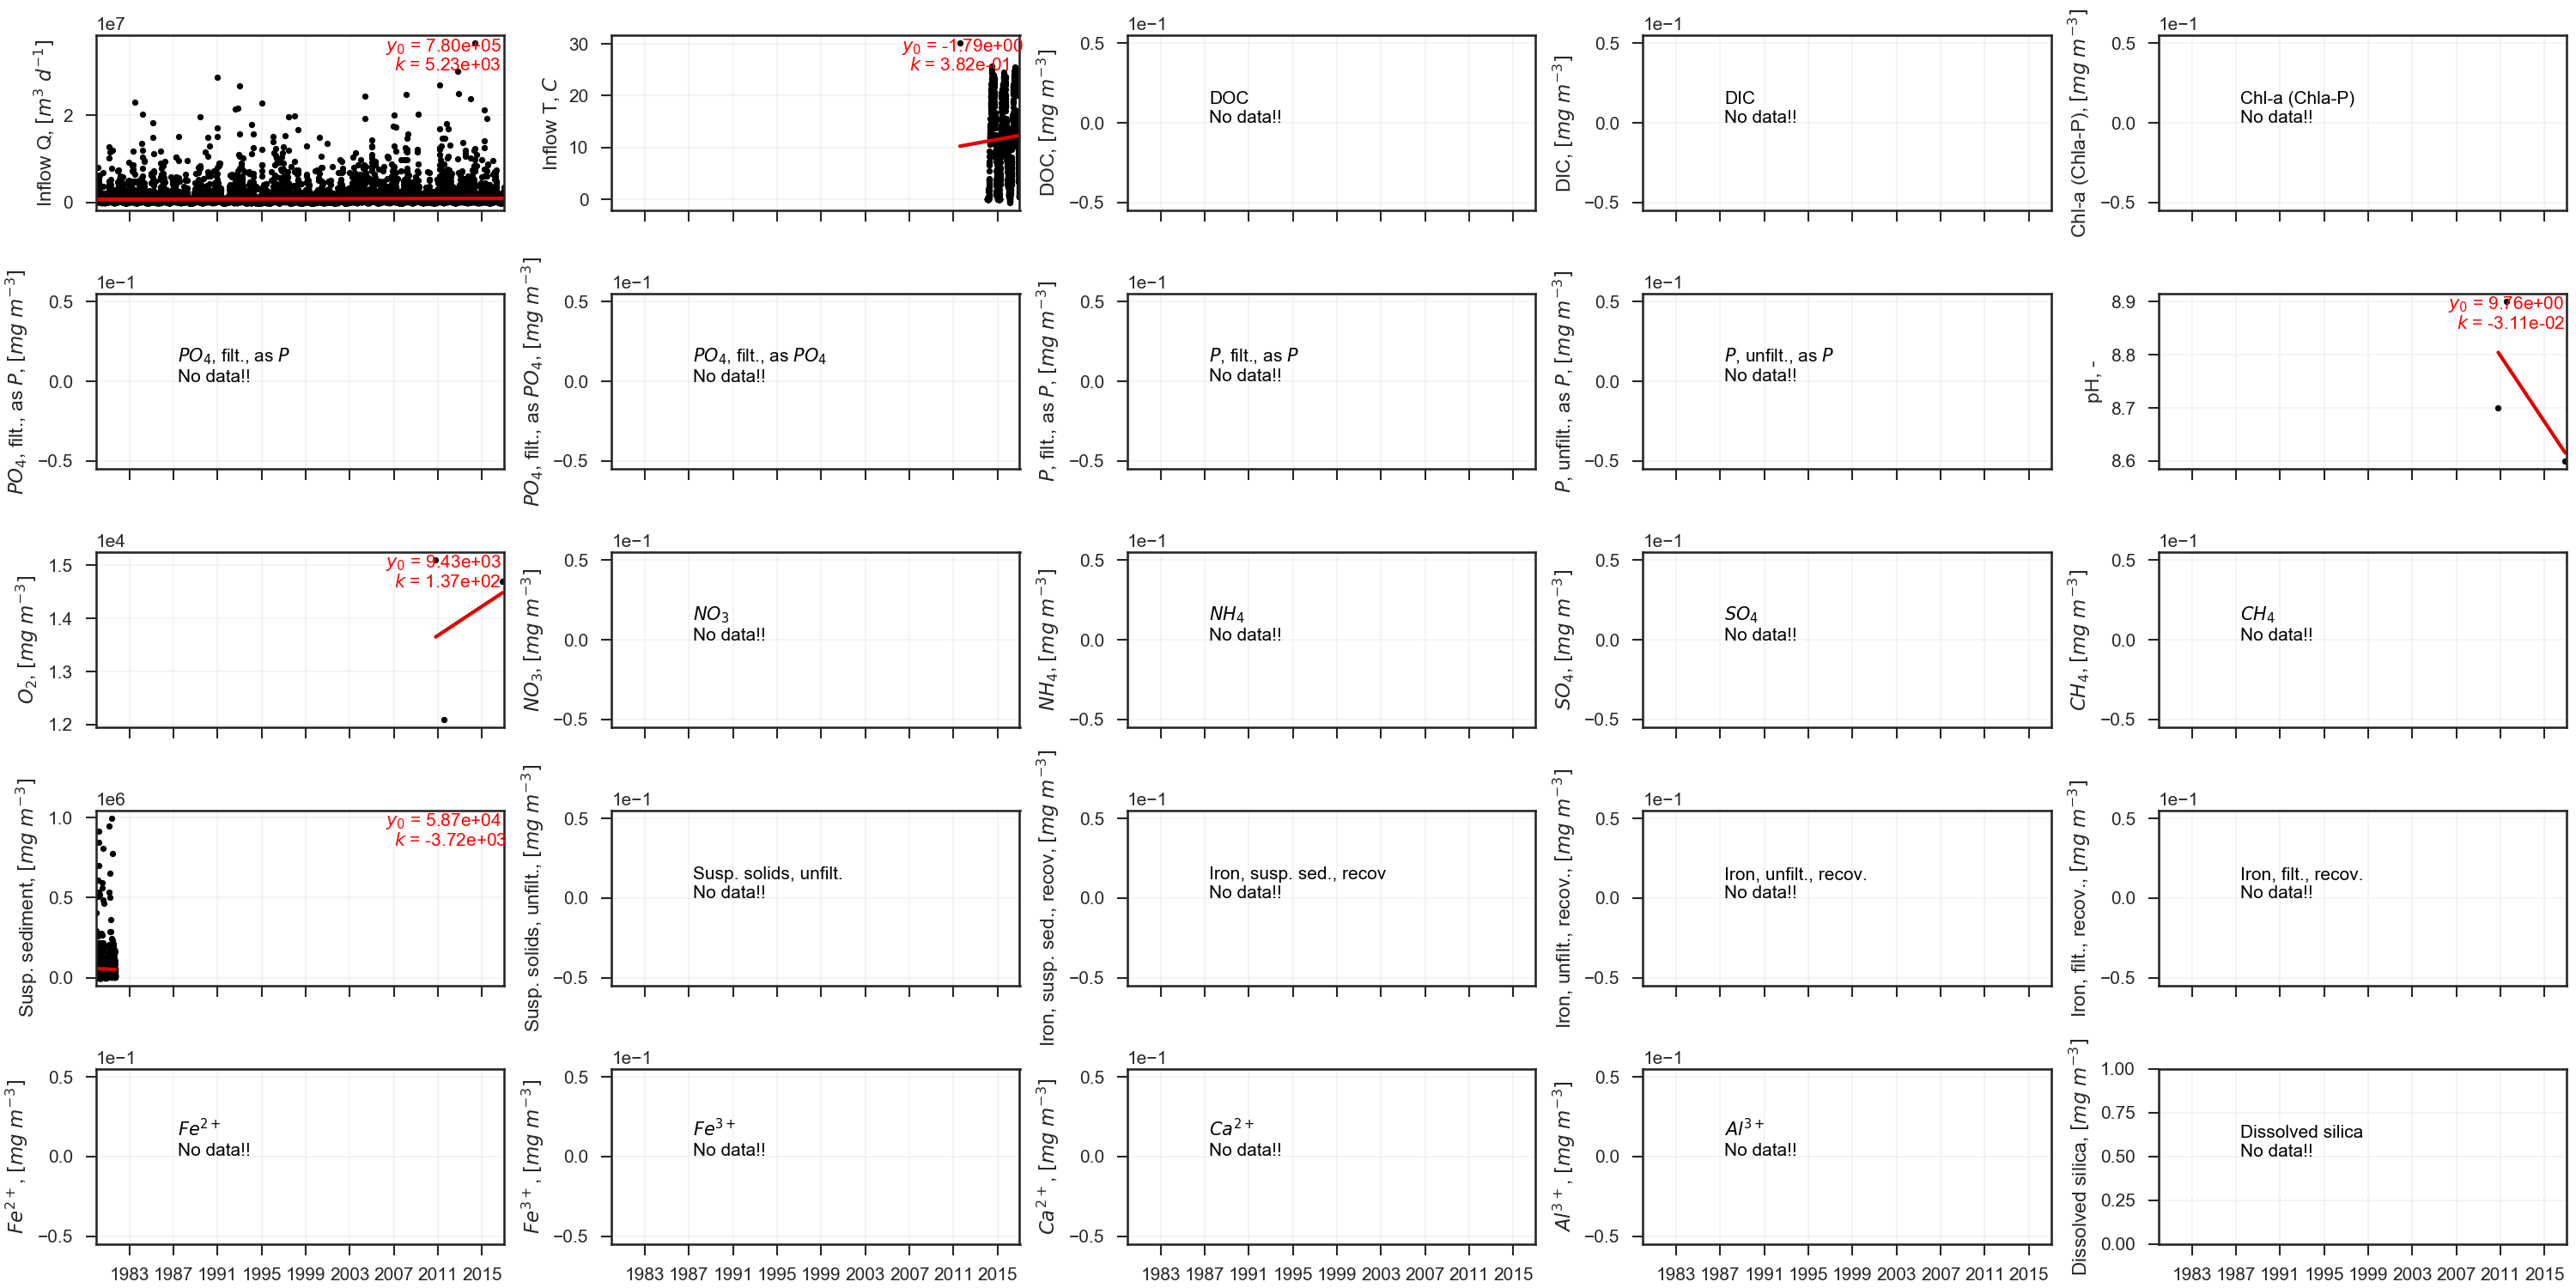
\includegraphics[width=\textwidth]{rivers/Central basin/plot_all rockyriver.png}
\end{figure}
\end{frame}

\begin{frame}
\frametitle{Central Basin: Sandusky river}
\begin{figure}
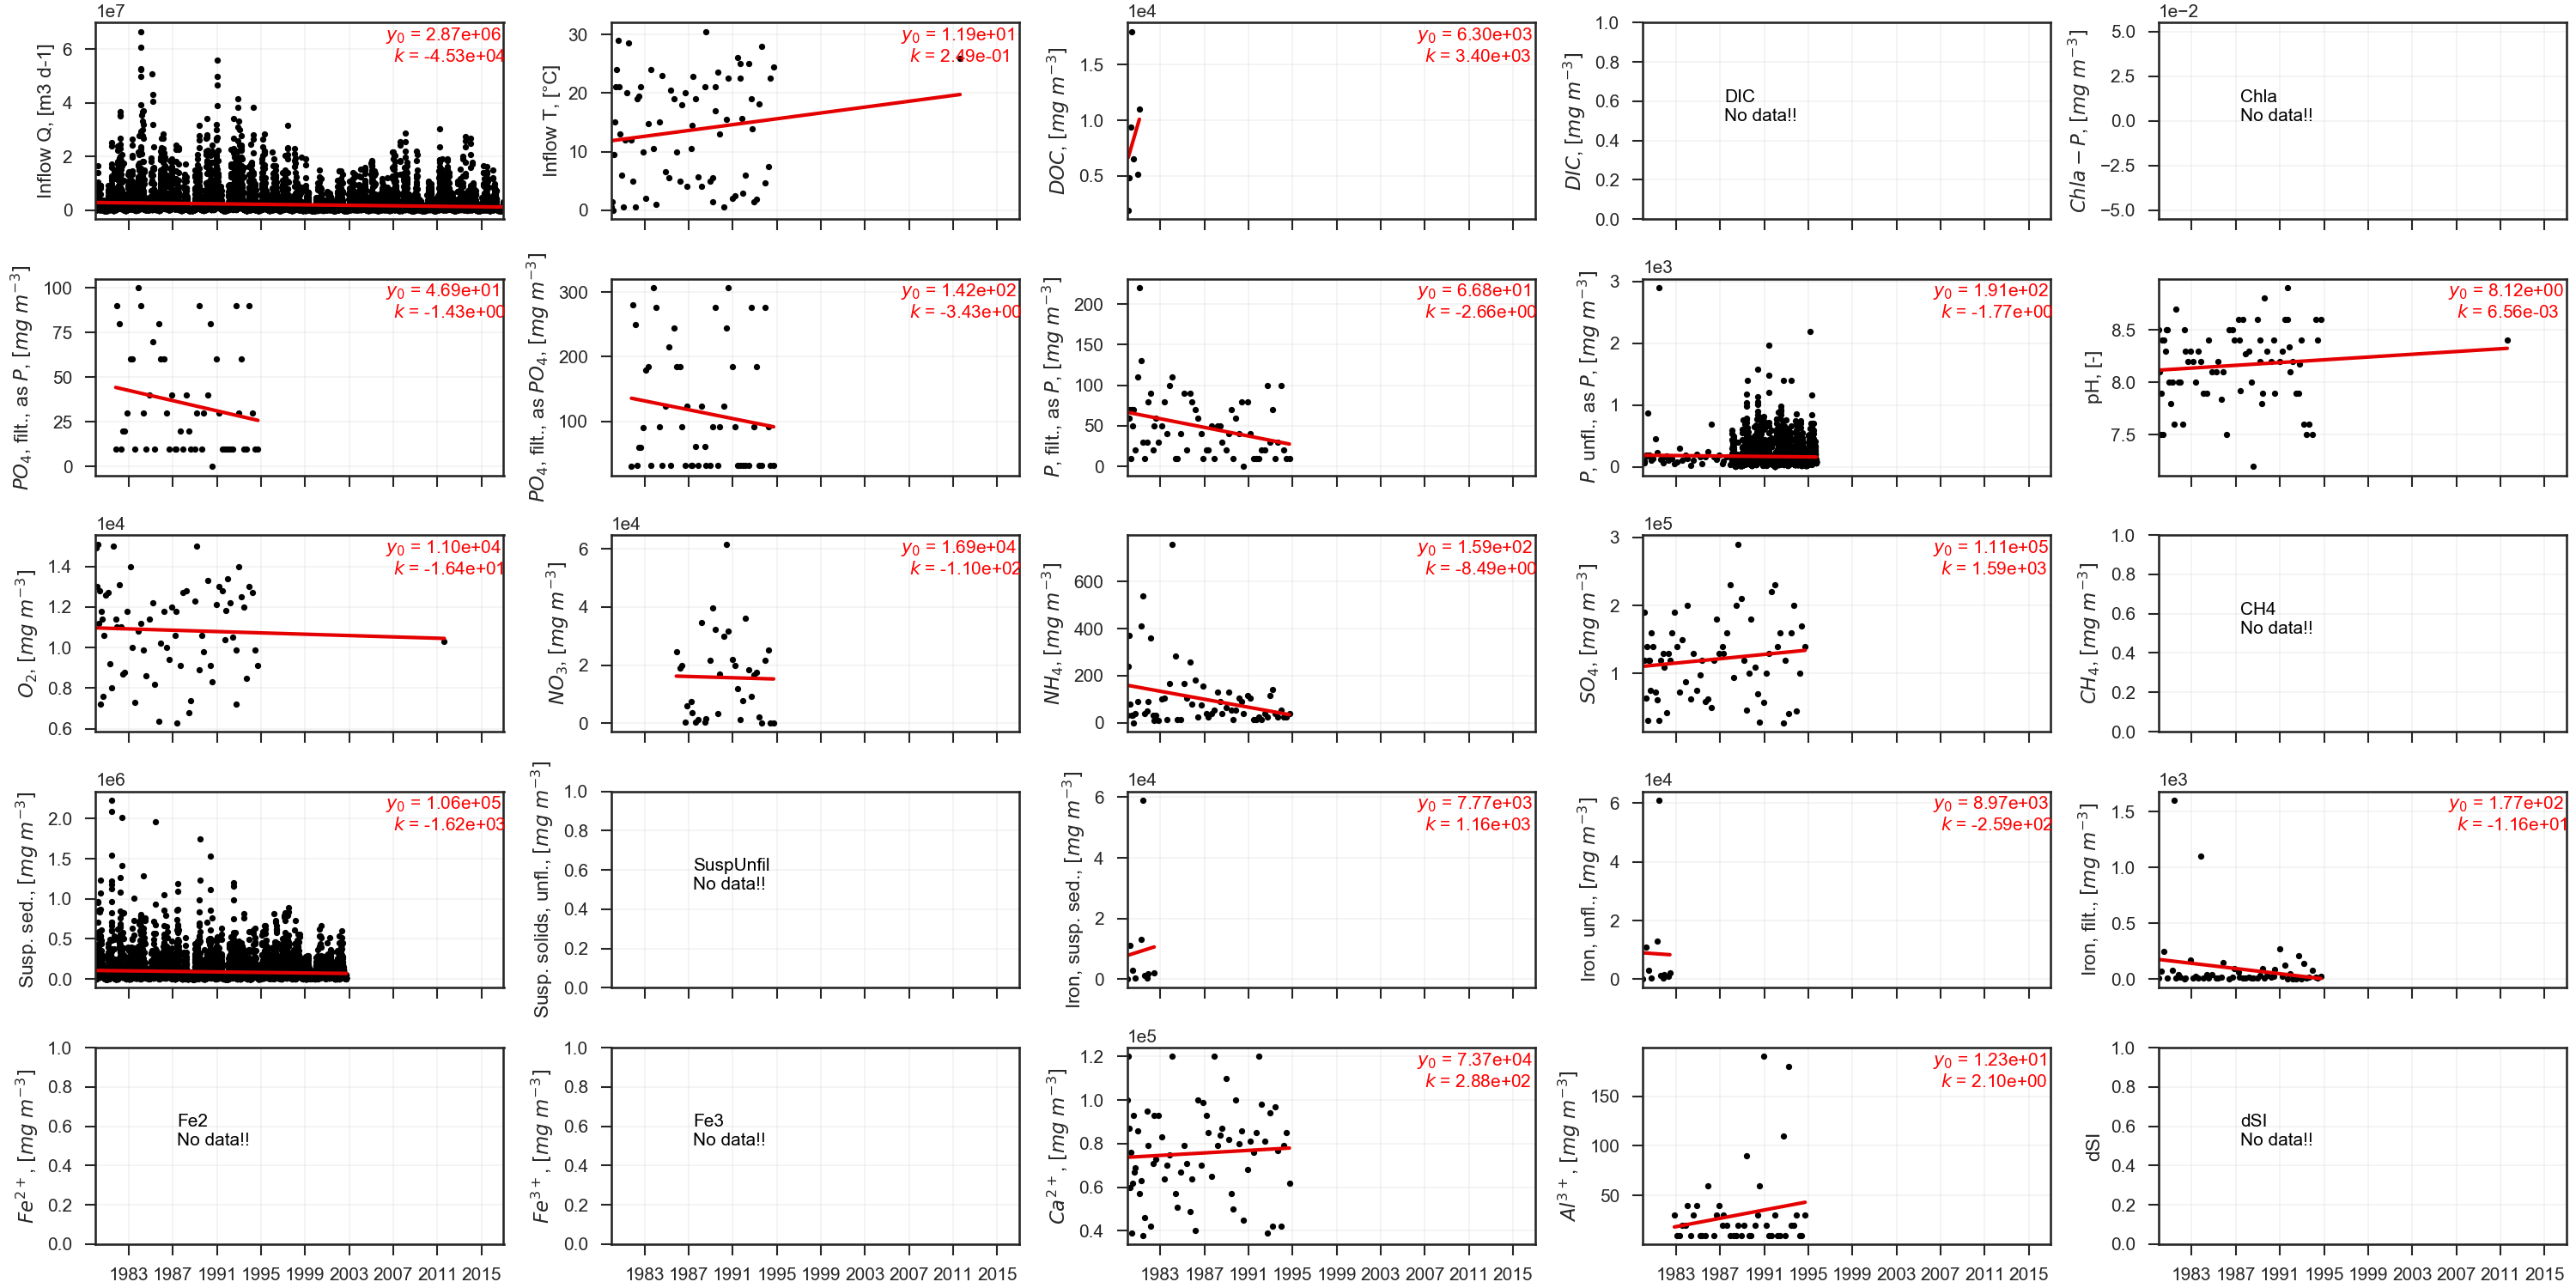
\includegraphics[width=\textwidth]{rivers/Central basin/plot_all sanduskyriver.png}
\end{figure}
\end{frame}

\begin{frame}
\frametitle{Central Basin: South-western Huron river}
\begin{figure}
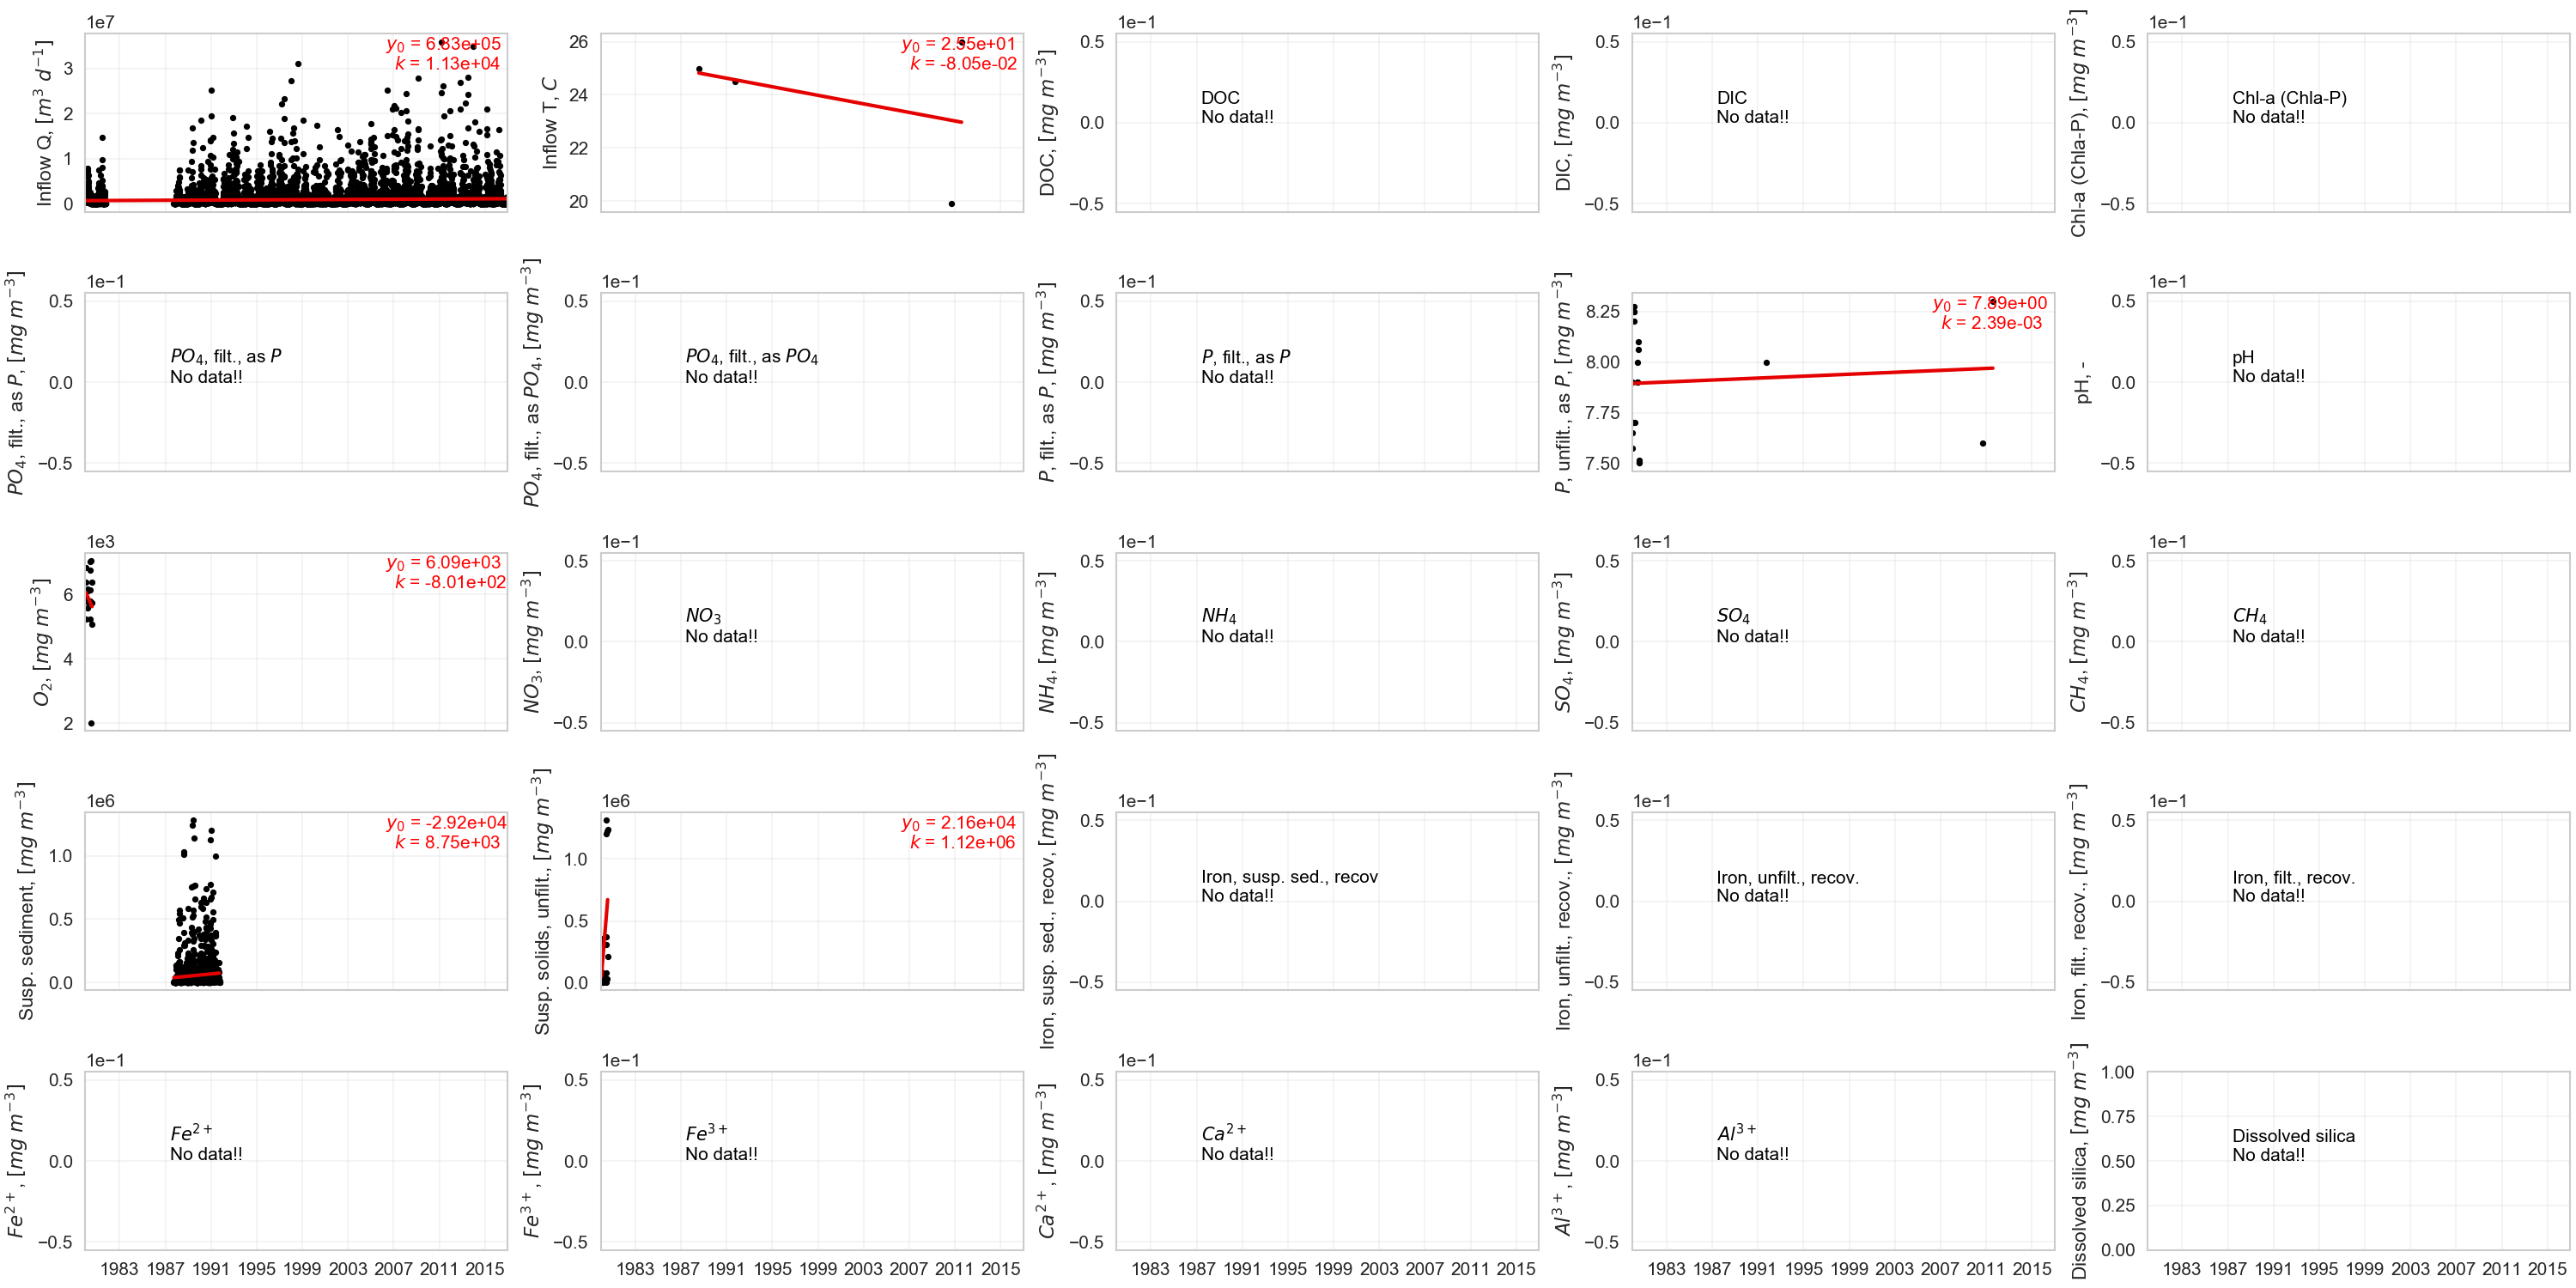
\includegraphics[width=\textwidth]{rivers/Central basin/plot_all southwesternhuronriver.png}
\end{figure}
\end{frame}

\begin{frame}
\frametitle{Central Basin: Vermillion river}
\begin{figure}
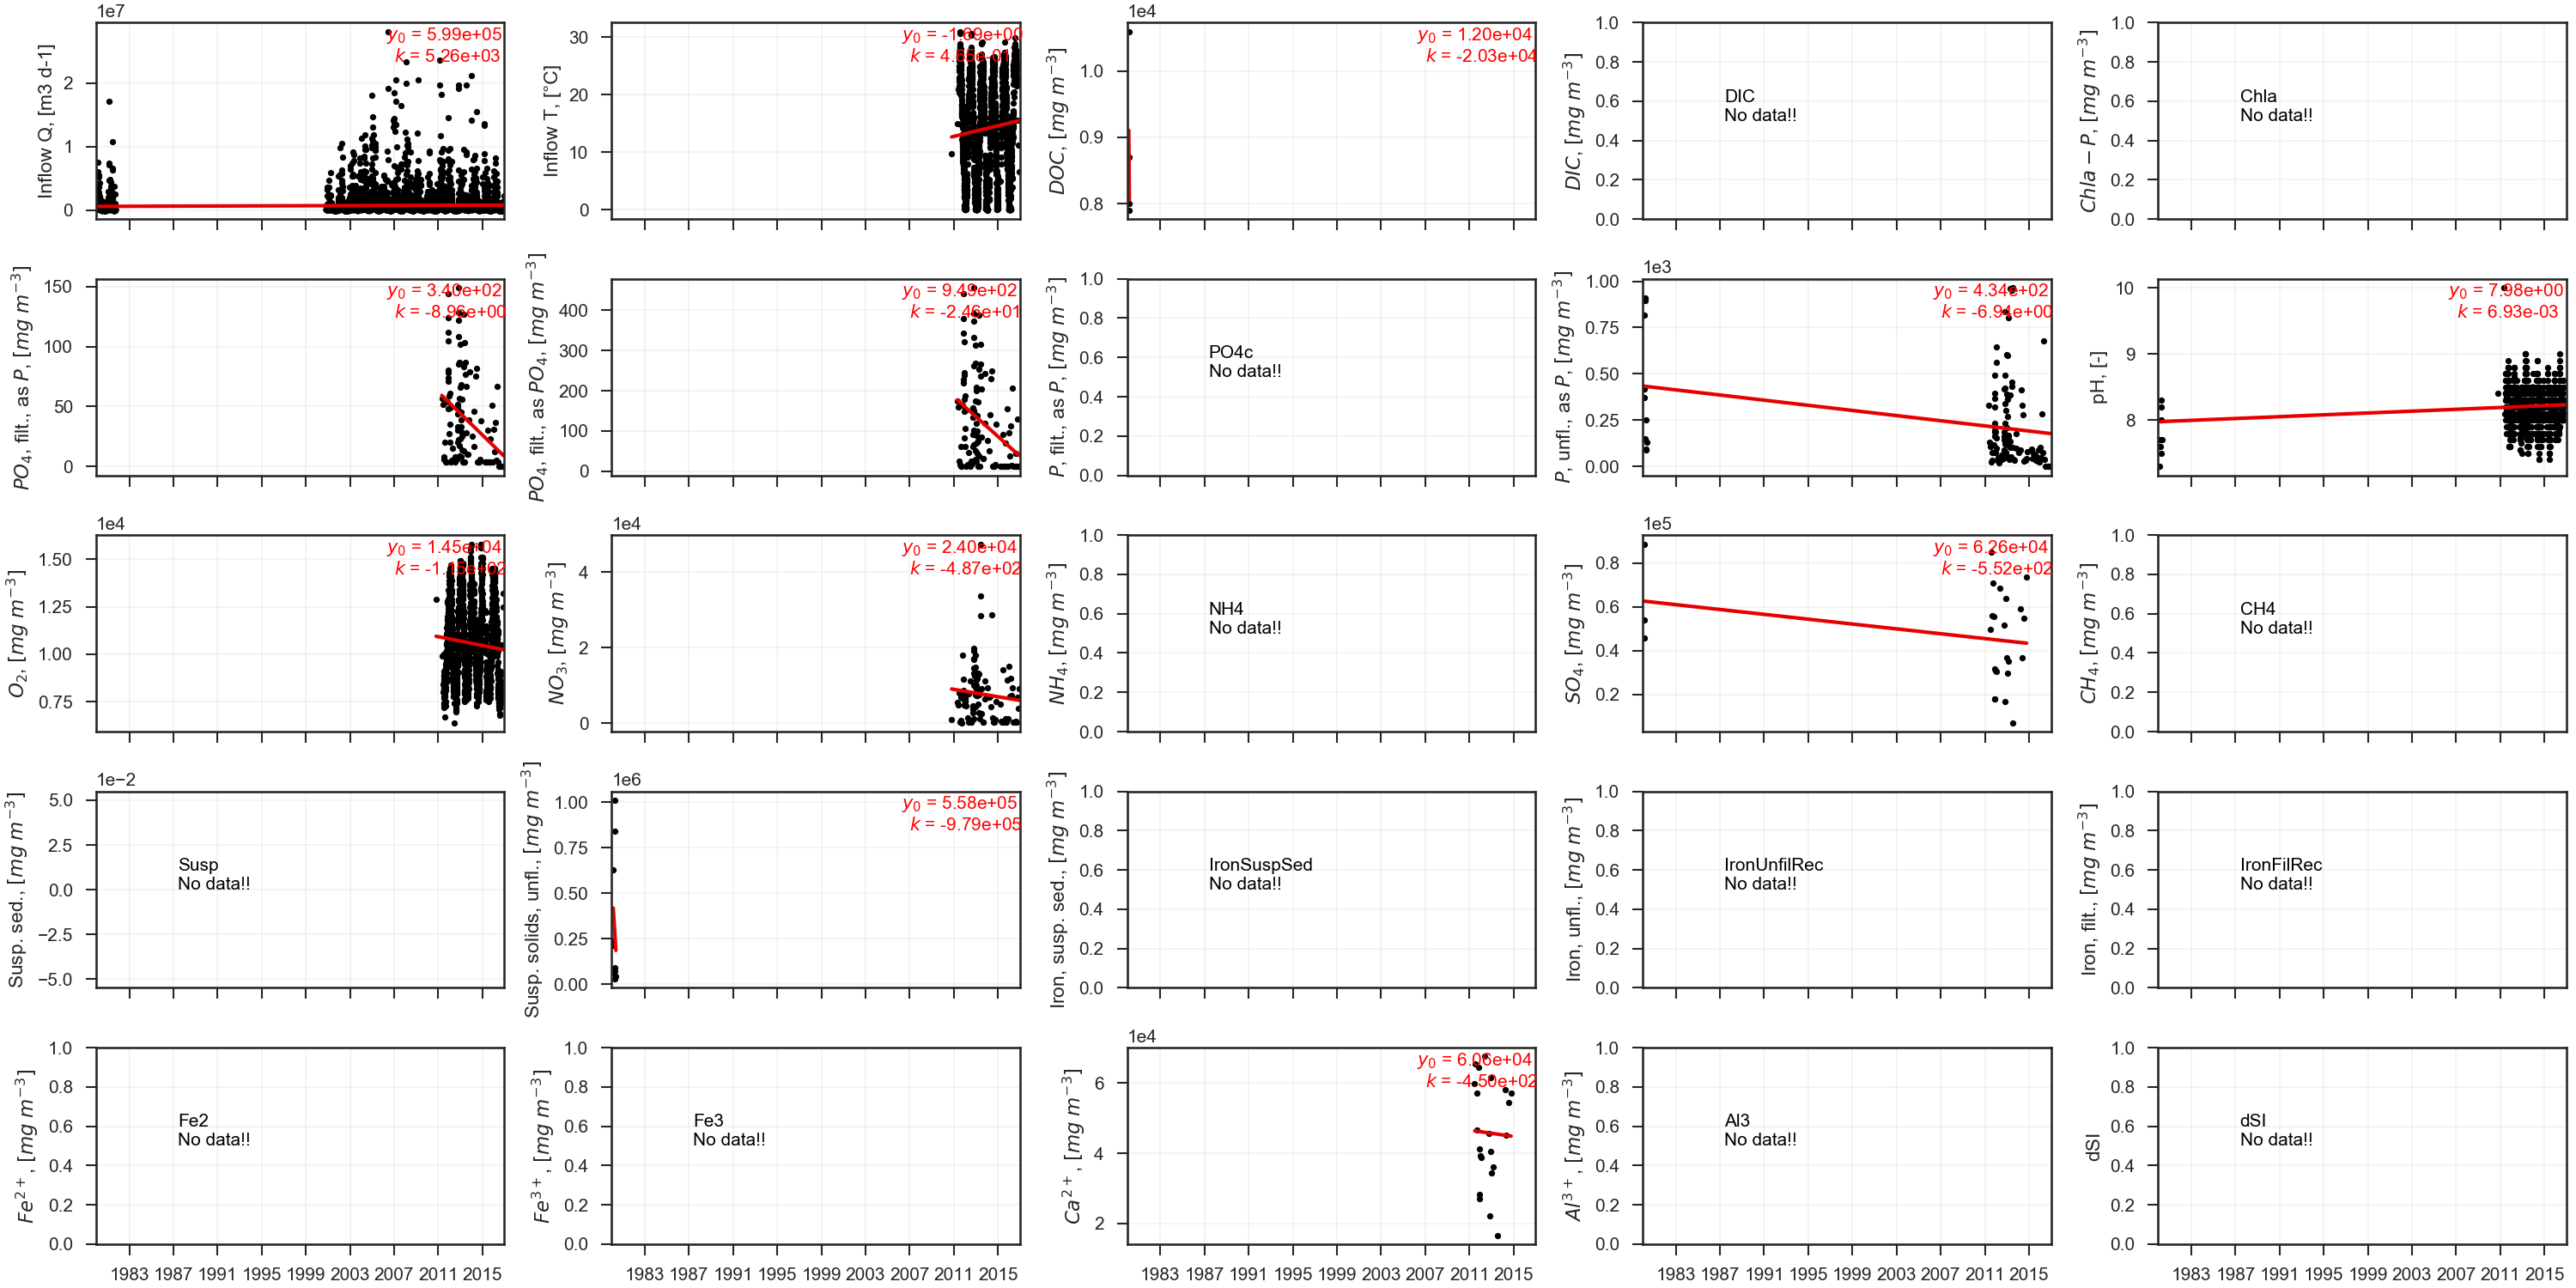
\includegraphics[width=\textwidth]{rivers/Central basin/plot_all vermillion.png}
\end{figure}
\end{frame}


\subsection{Eastern Basin}
\label{sub:eastern_basin}


\begin{frame}
\frametitle{Eastern Basin: Niagara river}
\begin{figure}
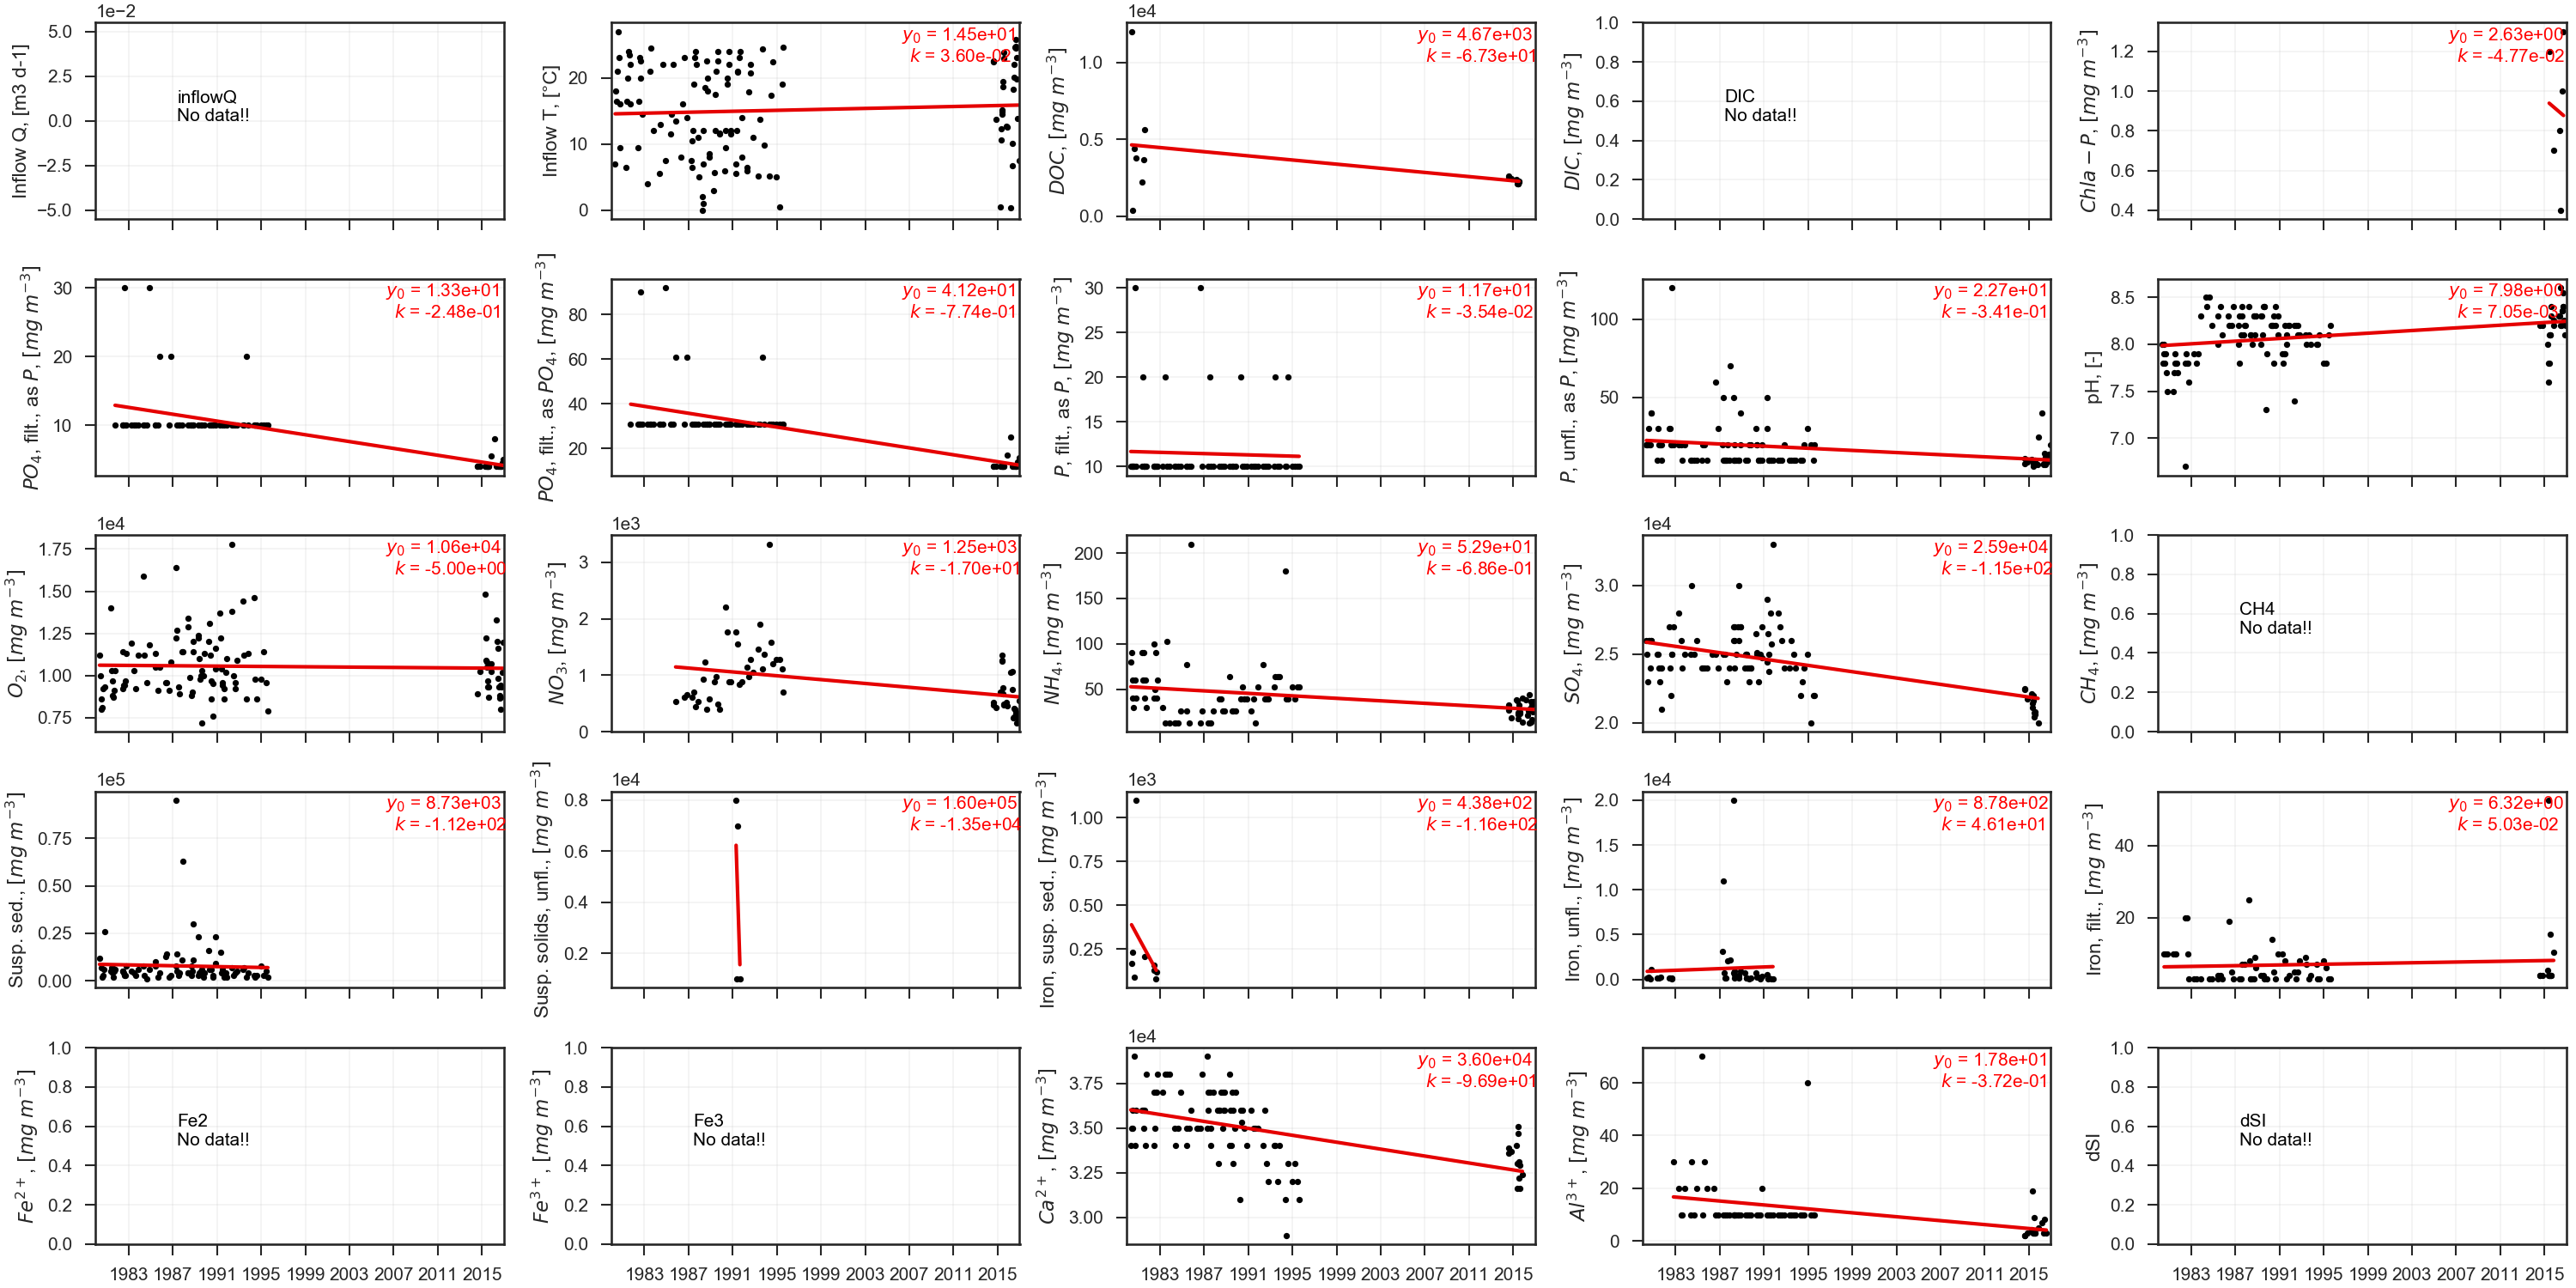
\includegraphics[width=\textwidth]{rivers/Eastern basin/plot_all niagarariver.png}
\end{figure}
\end{frame}

\begin{frame}
\frametitle{Eastern Basin: Buffalo creek}
\begin{figure}
\includegraphics[width=\textwidth]{rivers/Eastern basin/plot_all Buffalocreek.png}
\end{figure}
\end{frame}

\begin{frame}
\frametitle{Eastern Basin: Cattaraugus creek}
\begin{figure}
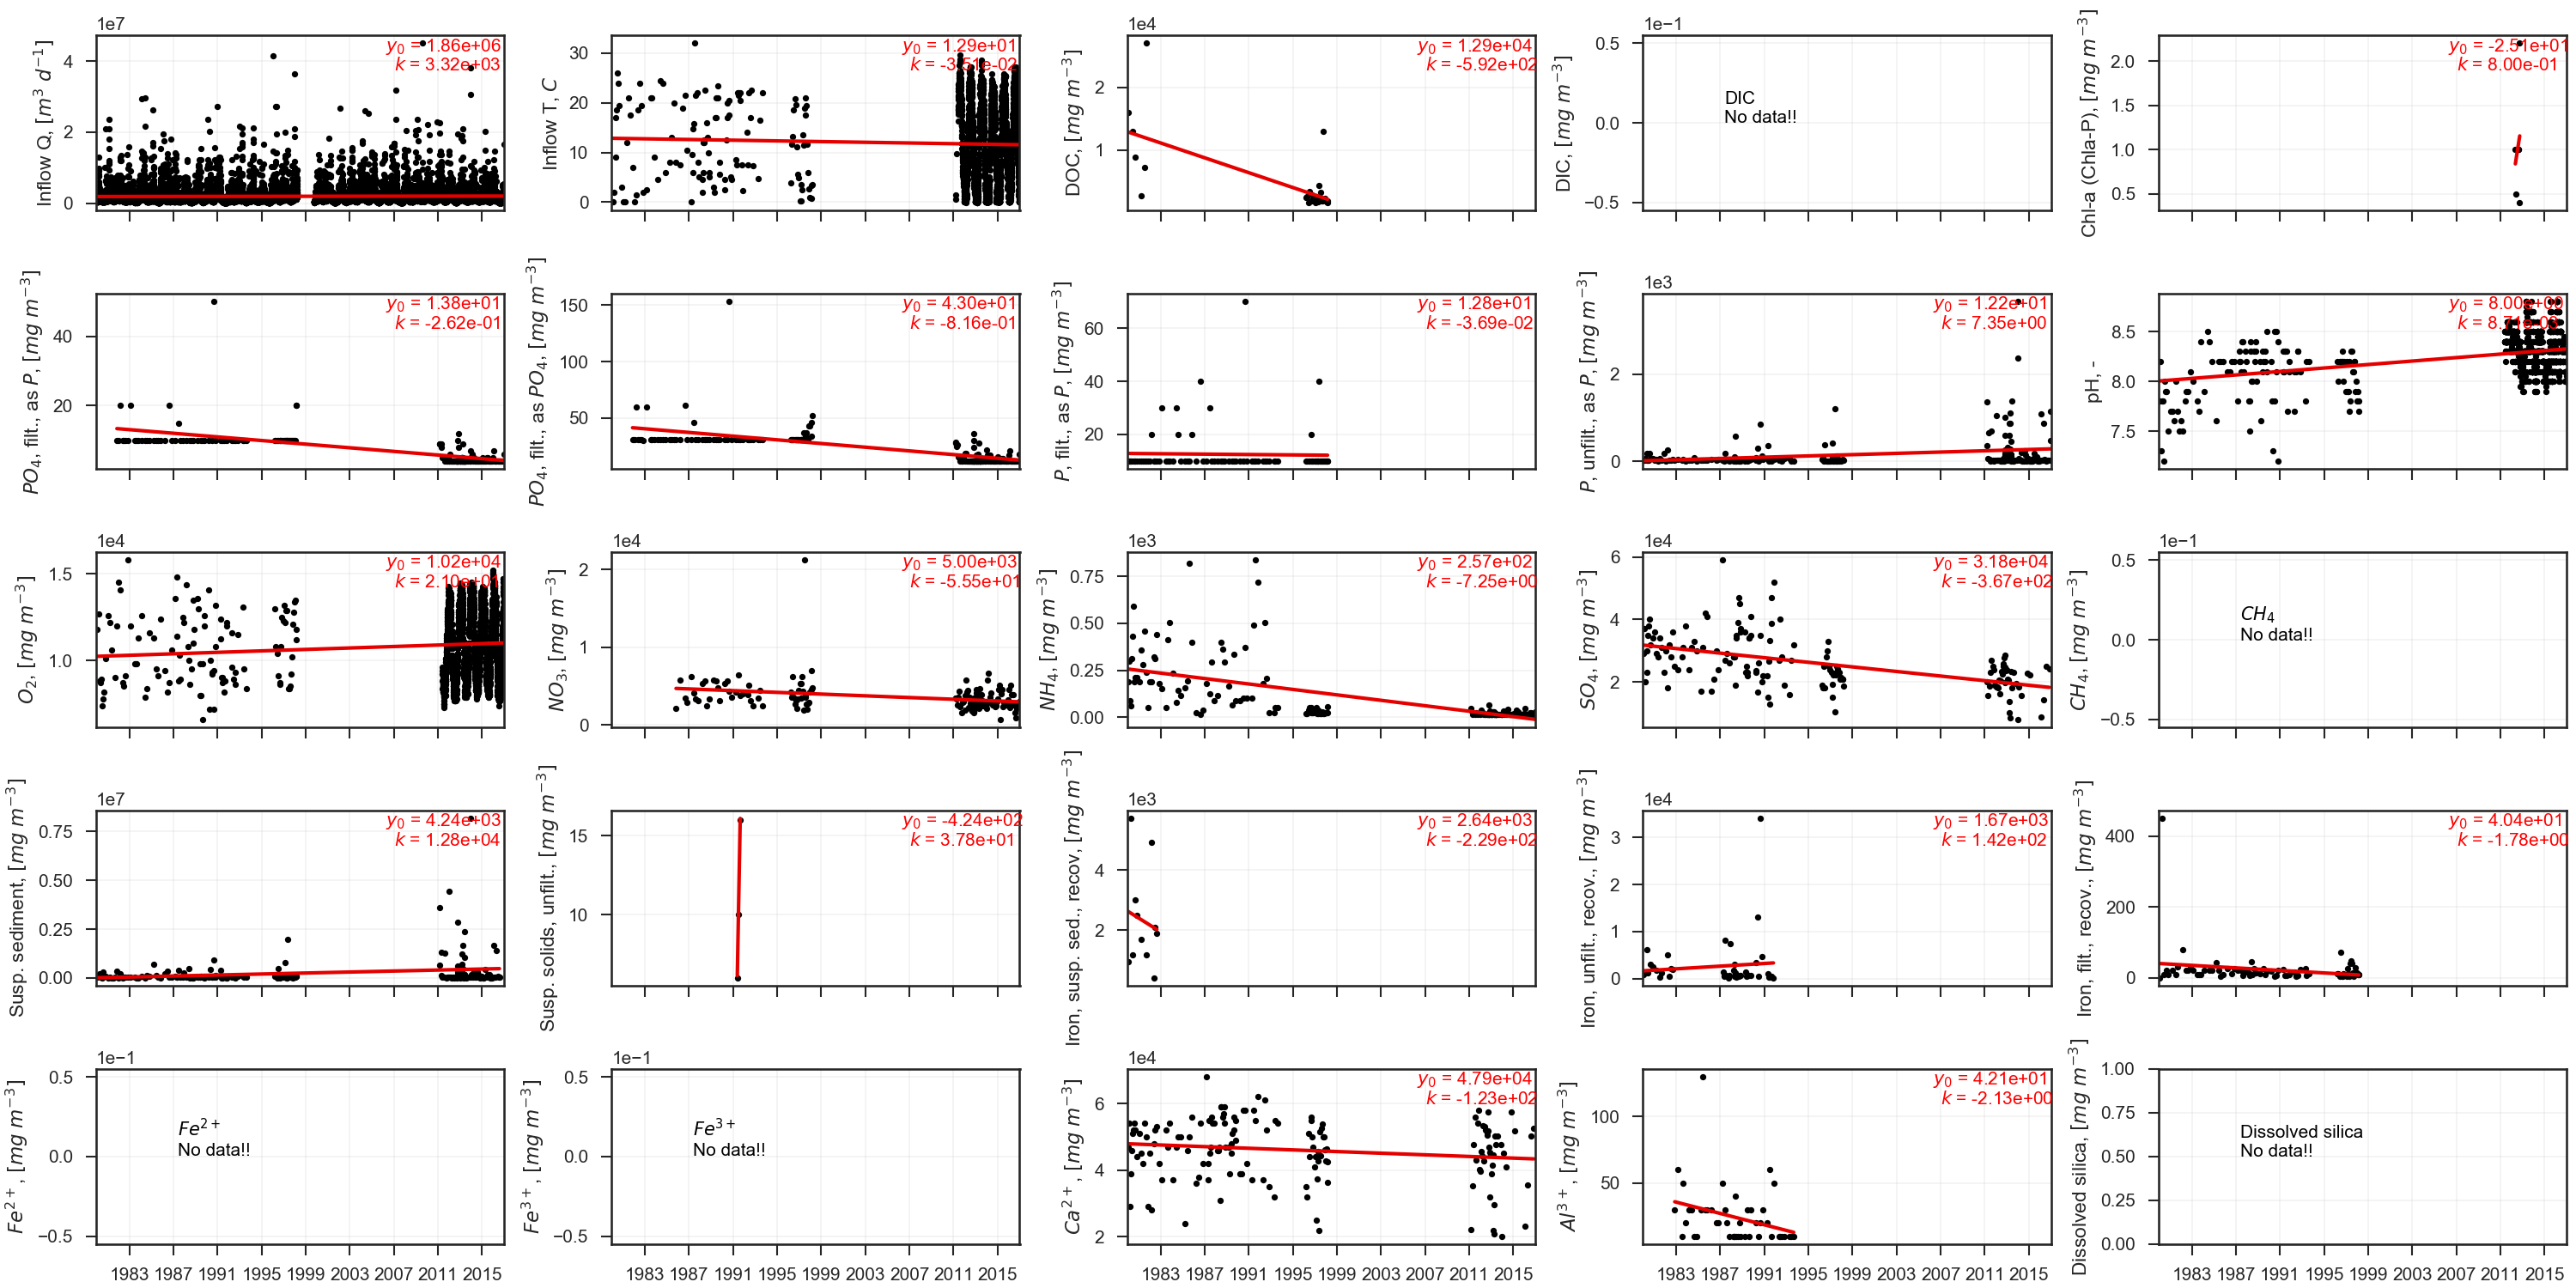
\includegraphics[width=\textwidth]{rivers/Eastern basin/plot_all cattarauguscreek.png}
\end{figure}
\end{frame}


\section{US Rivers' one year plots}
\label{sec:us_rivers_one_year_plots}

\subsection{Western Basin}
\label{sub:western_basin}

\begin{frame}
\frametitle{Western Basin: Detroit river}
\begin{figure}
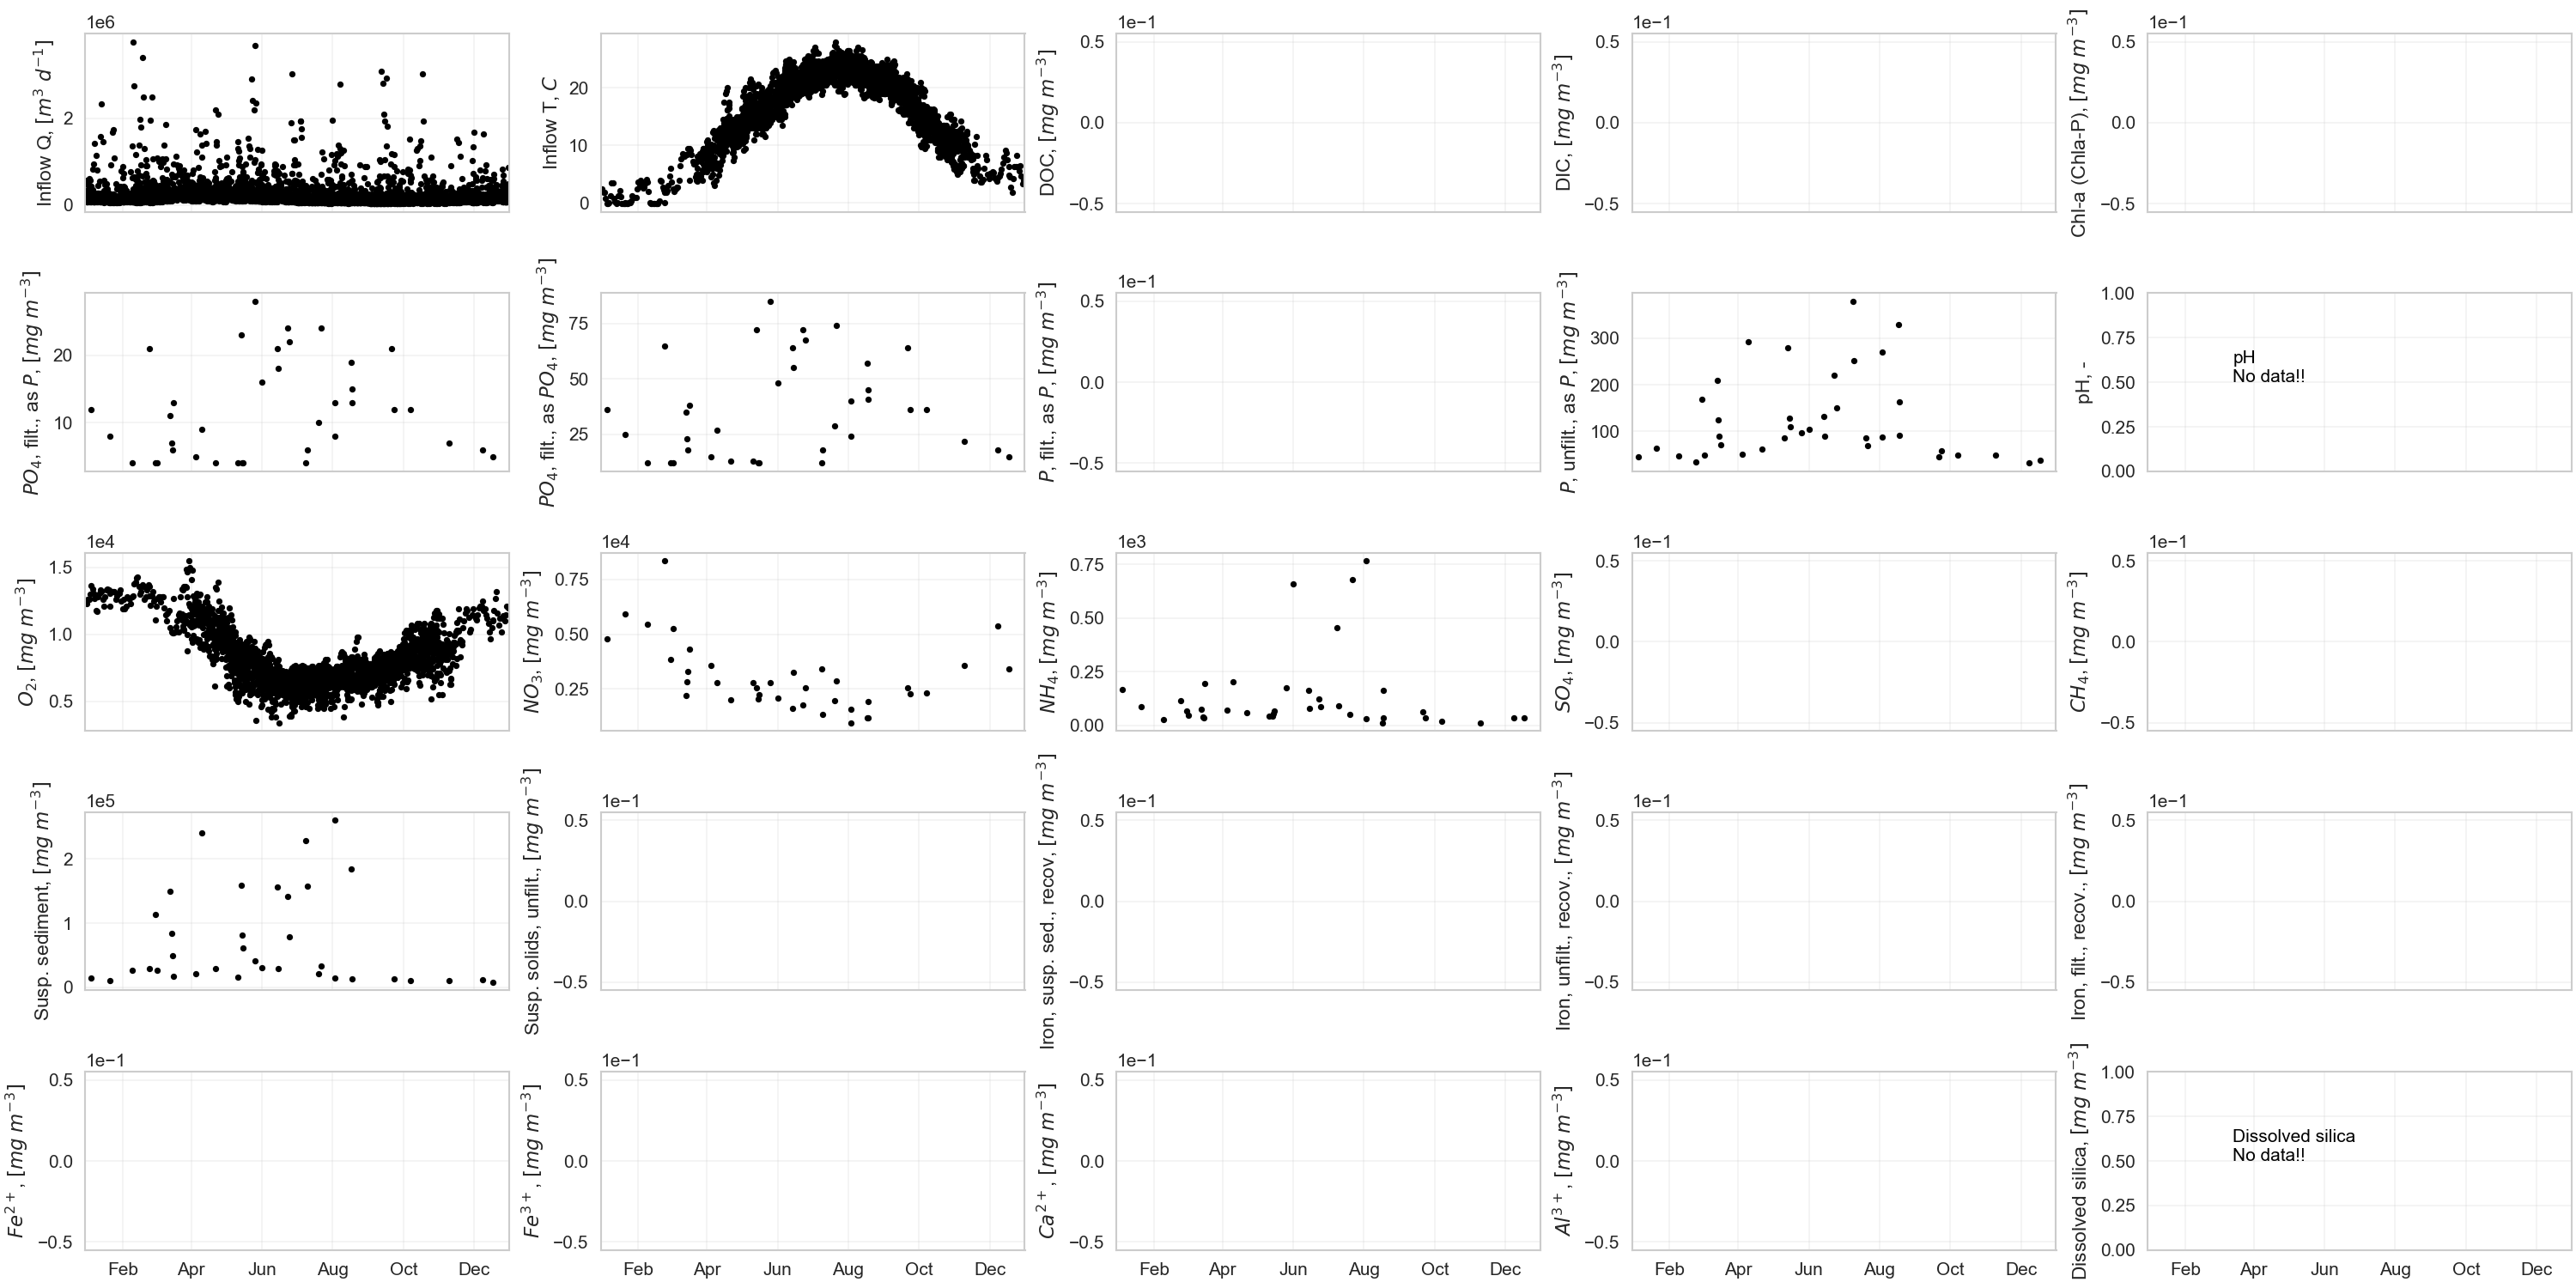
\includegraphics[width=\textwidth]{rivers/Western basin/plot_1yr detroitriver.png}
\end{figure}
\end{frame}


\begin{frame}
\frametitle{Western Basin: Huron river}
\begin{figure}
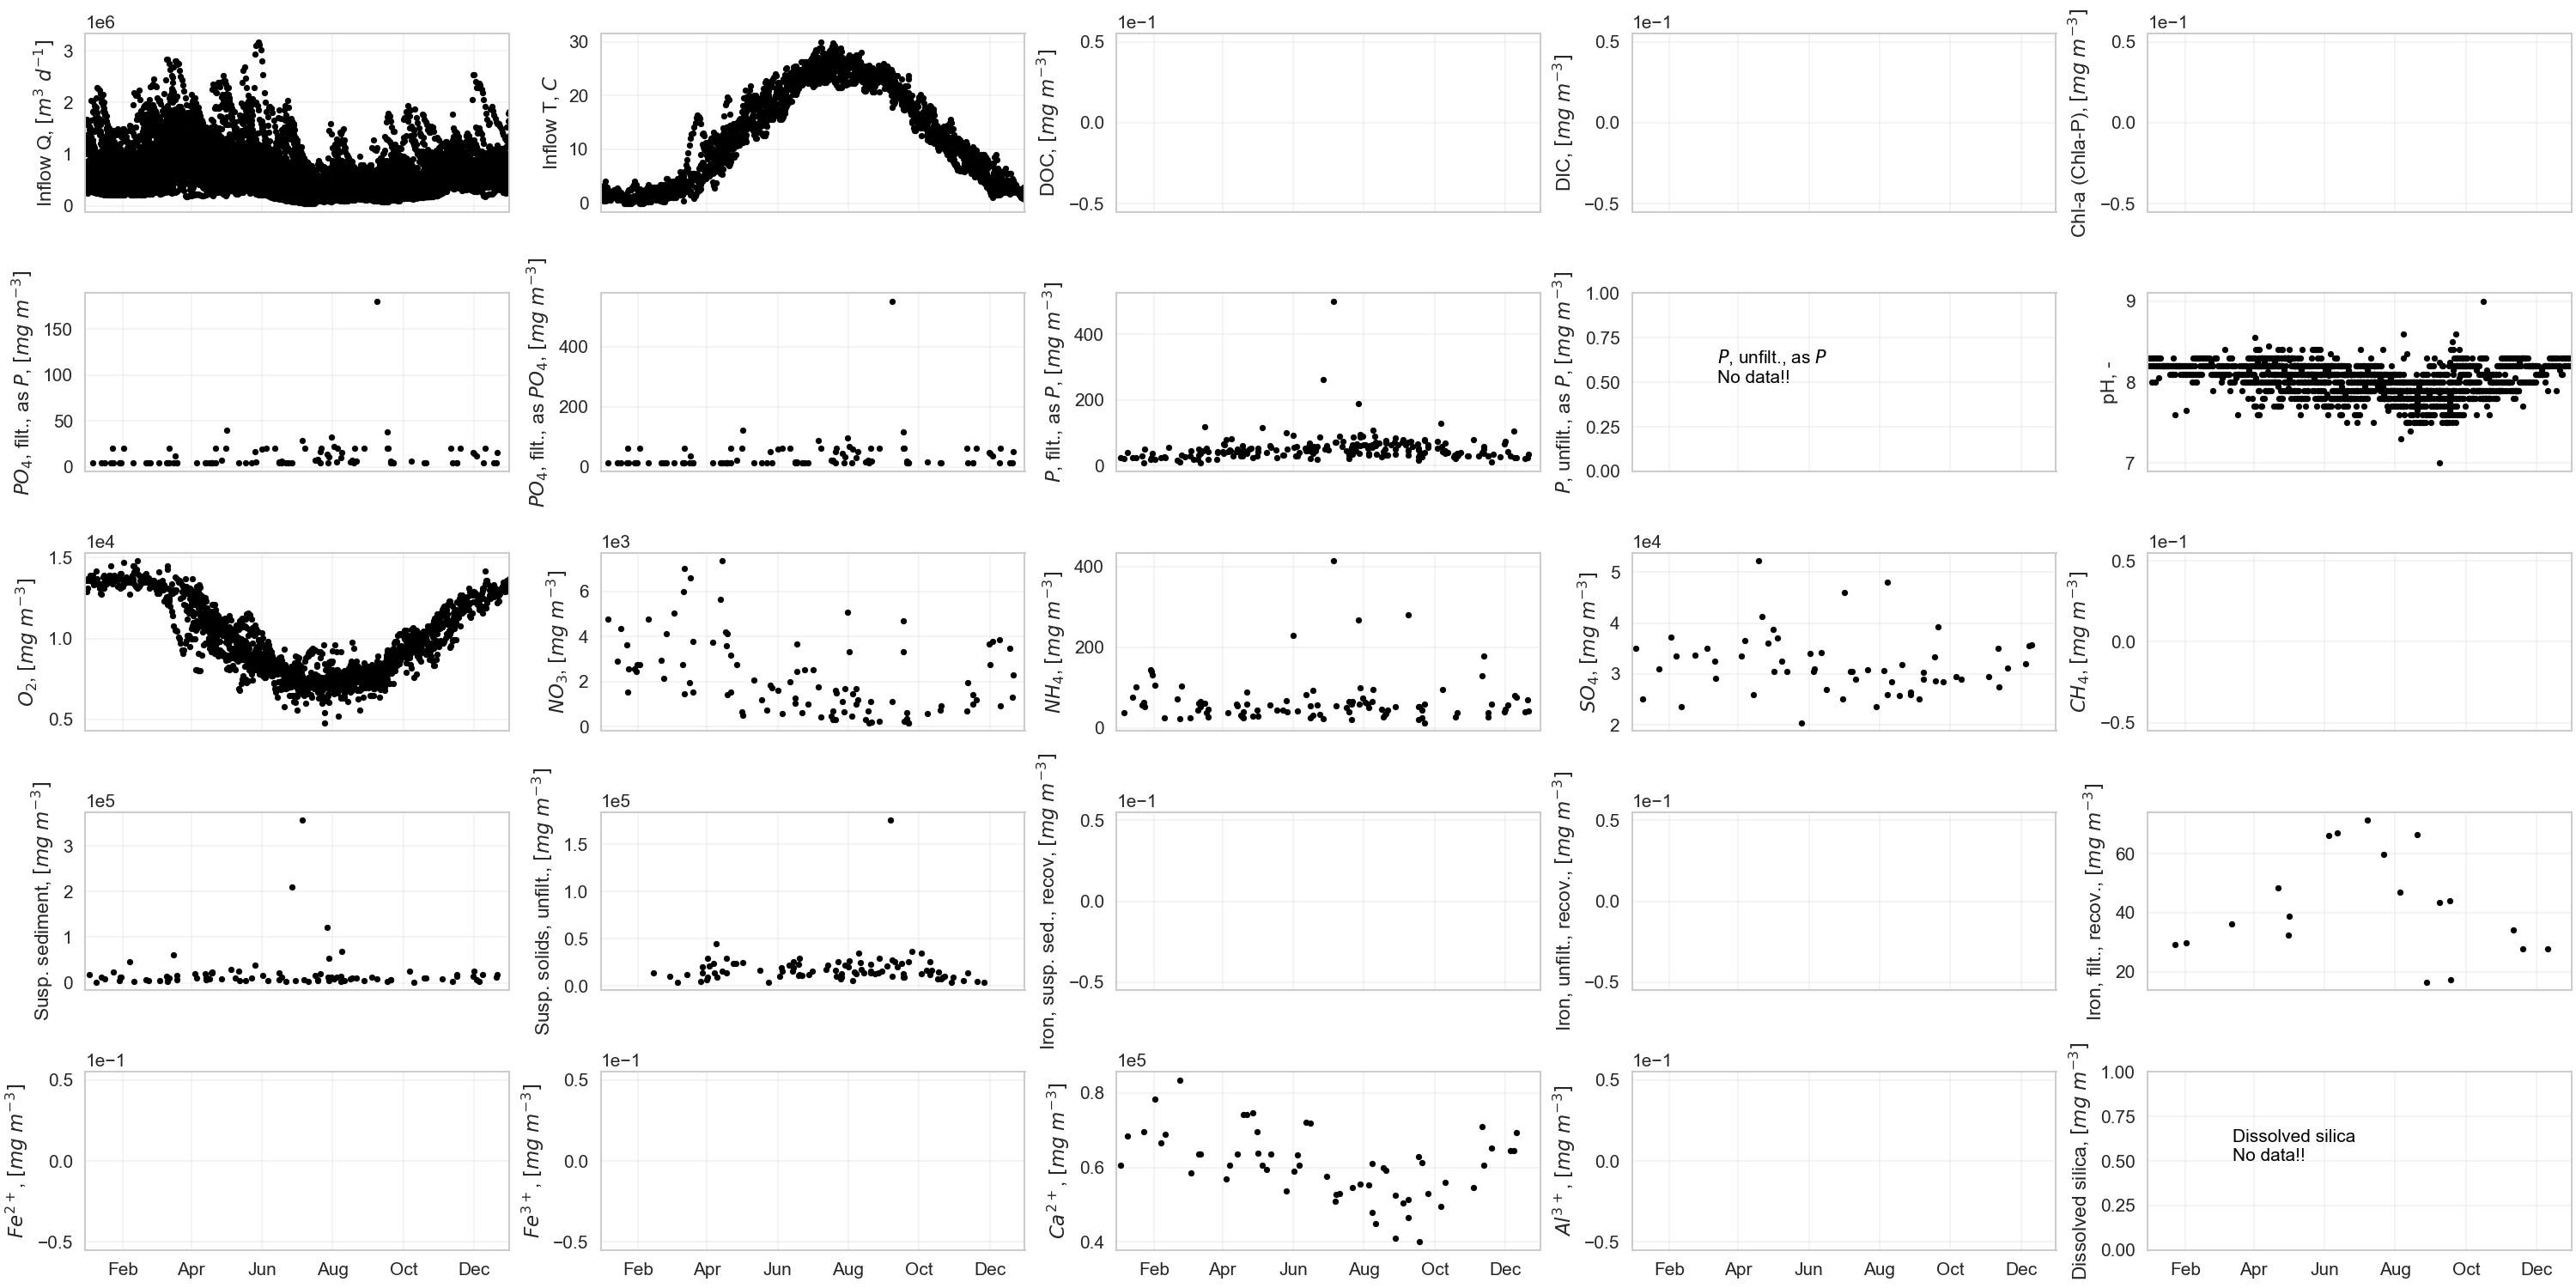
\includegraphics[width=\textwidth]{rivers/Western basin/plot_1yr huronriver.png}
\end{figure}
\end{frame}


\begin{frame}
\frametitle{Western Basin: Maumee river}
\begin{figure}
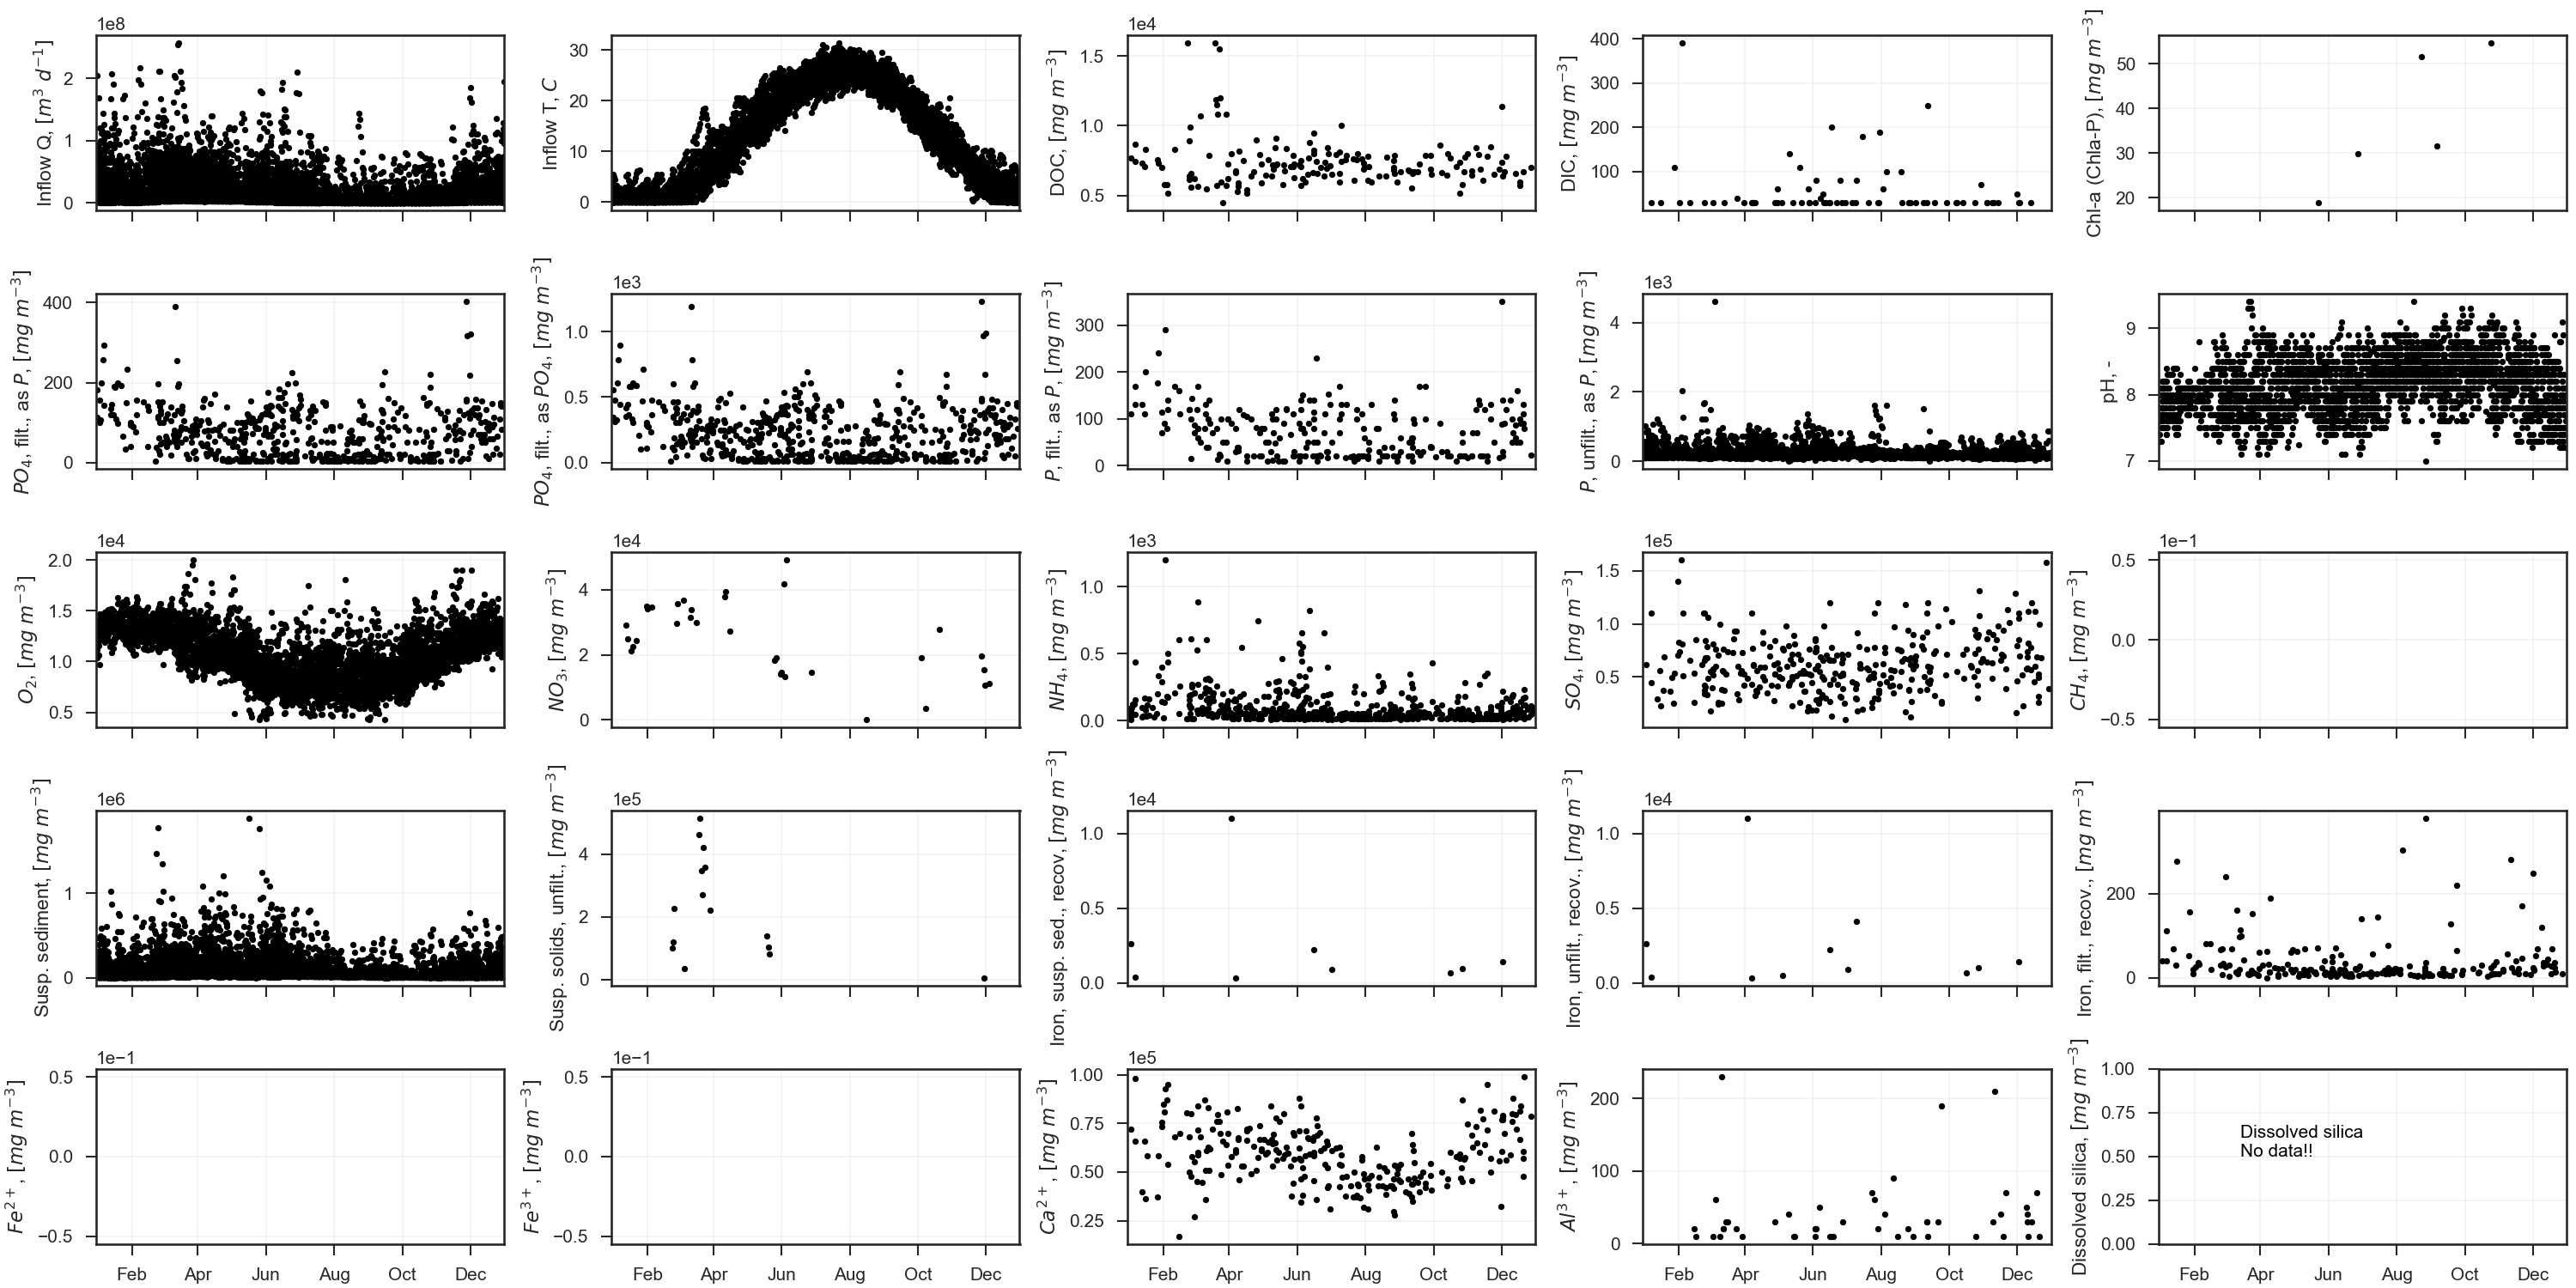
\includegraphics[width=\textwidth]{rivers/Western basin/plot_1yr maumeeriver.png}
\end{figure}
\end{frame}


\begin{frame}
\frametitle{Western Basin: Ottawa river}
\begin{figure}
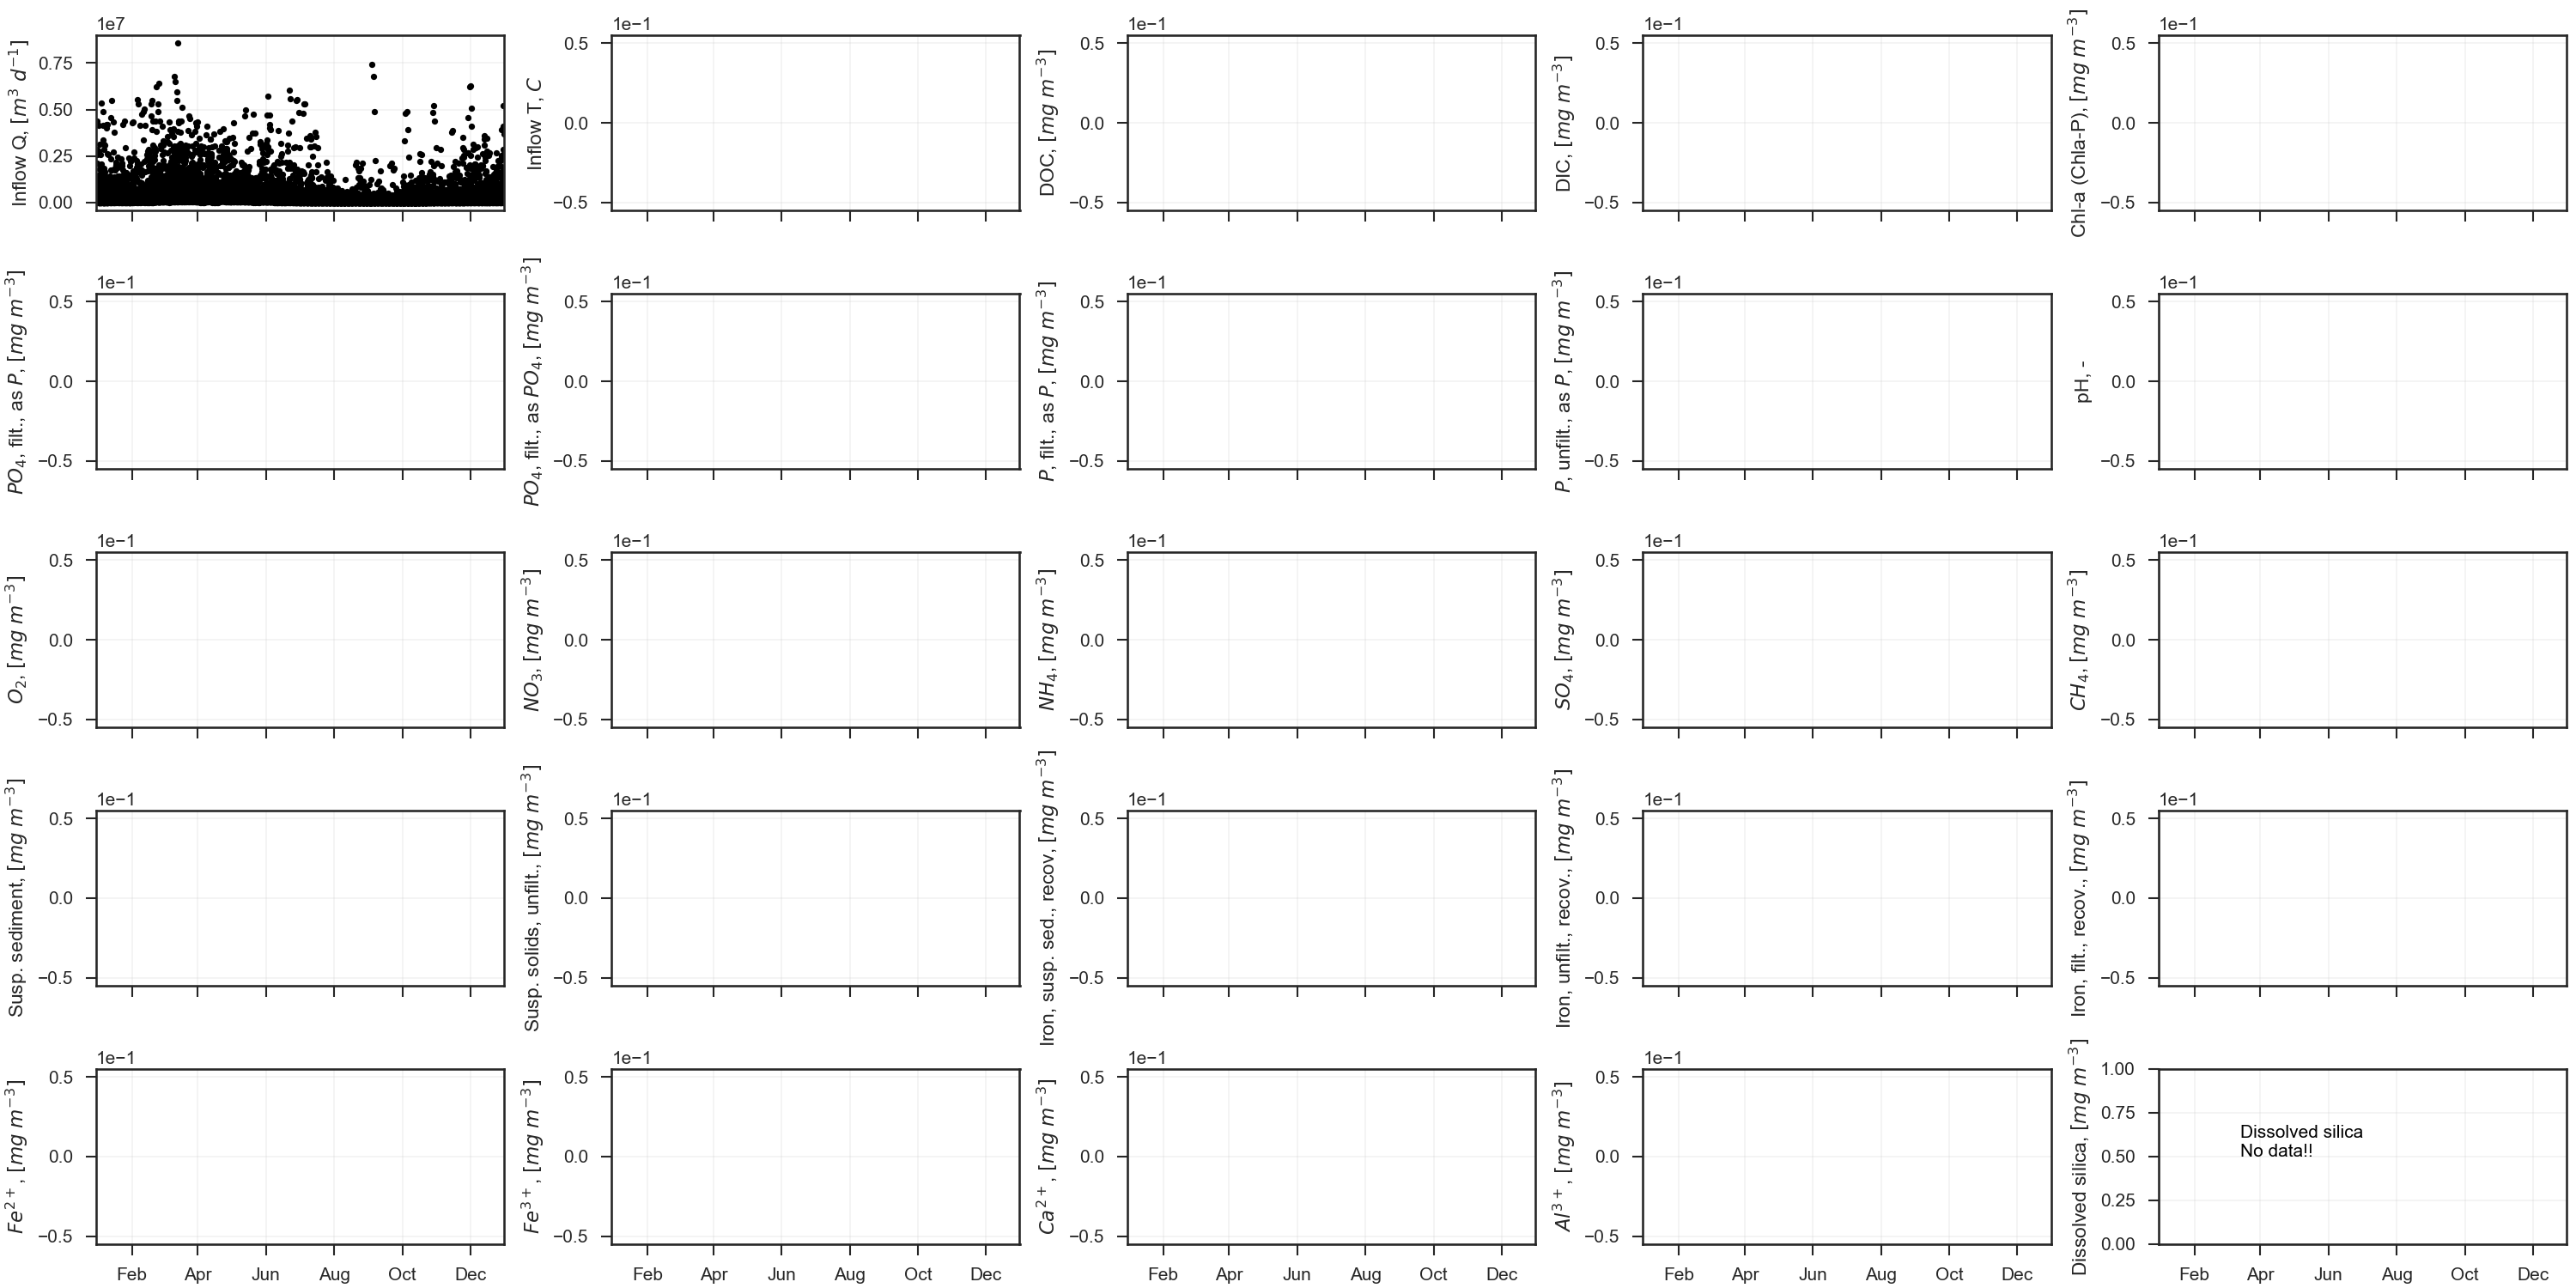
\includegraphics[width=\textwidth]{rivers/Western basin/plot_1yr ottawariver.png}
\end{figure}
\end{frame}


\begin{frame}
\frametitle{Western Basin: Portage river}
\begin{figure}
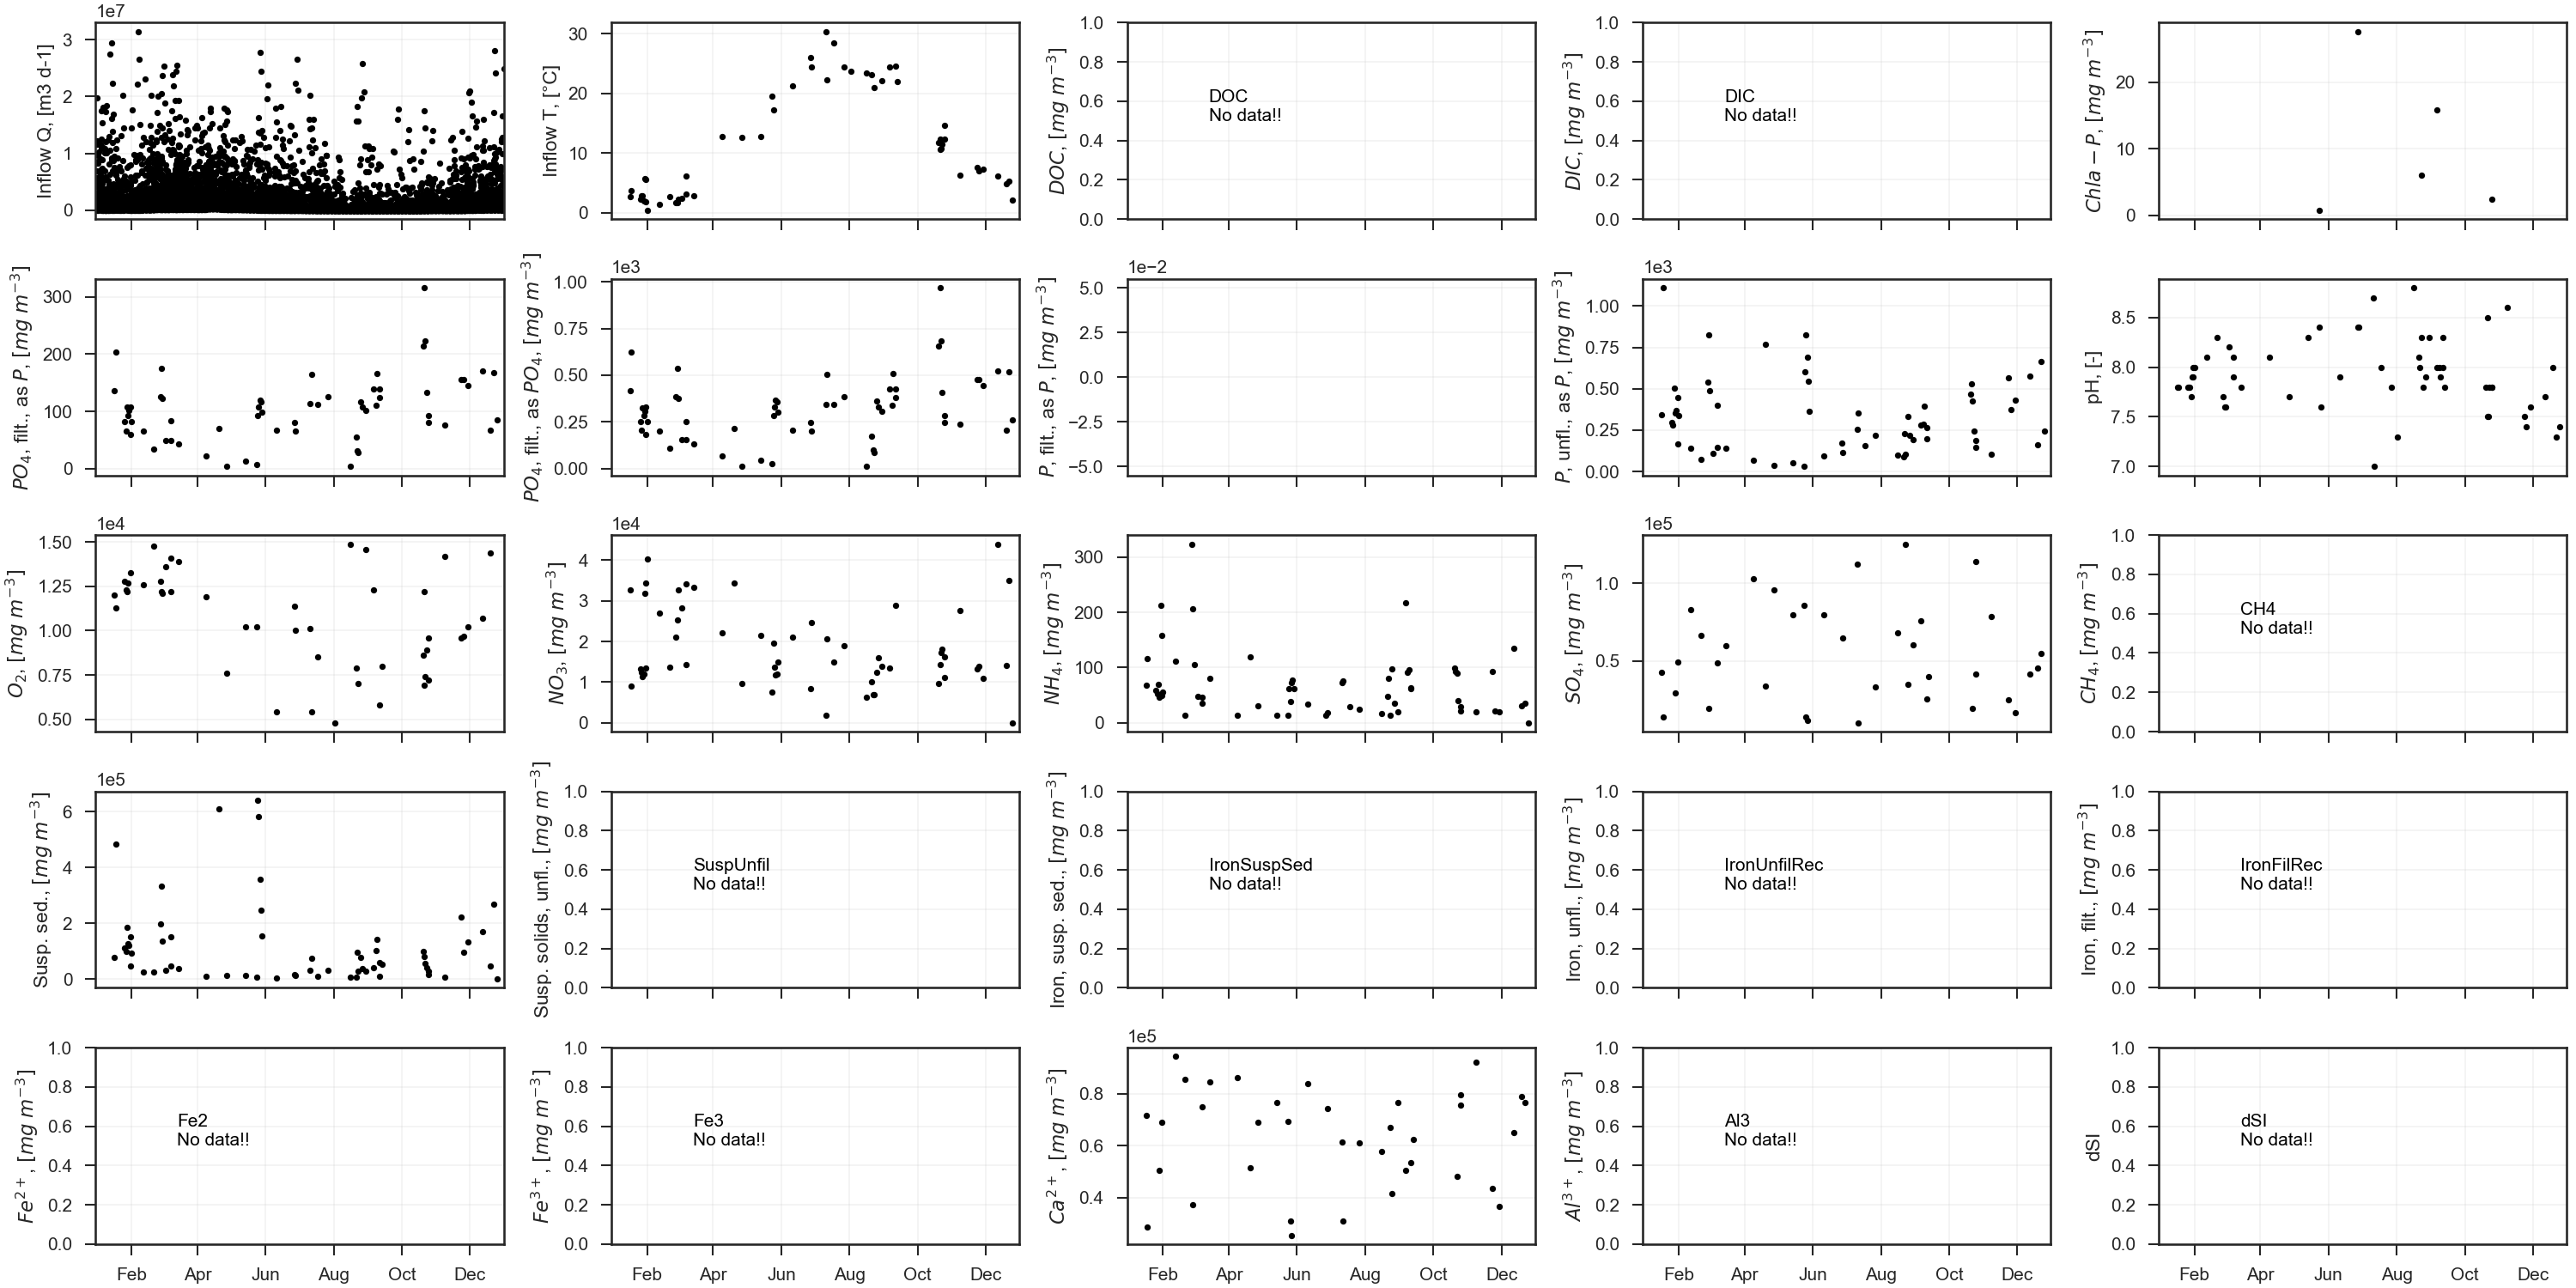
\includegraphics[width=\textwidth]{rivers/Western basin/plot_1yr portageriver.png}
\end{figure}
\end{frame}


\begin{frame}
\frametitle{Western Basin: Raisin river}
\begin{figure}
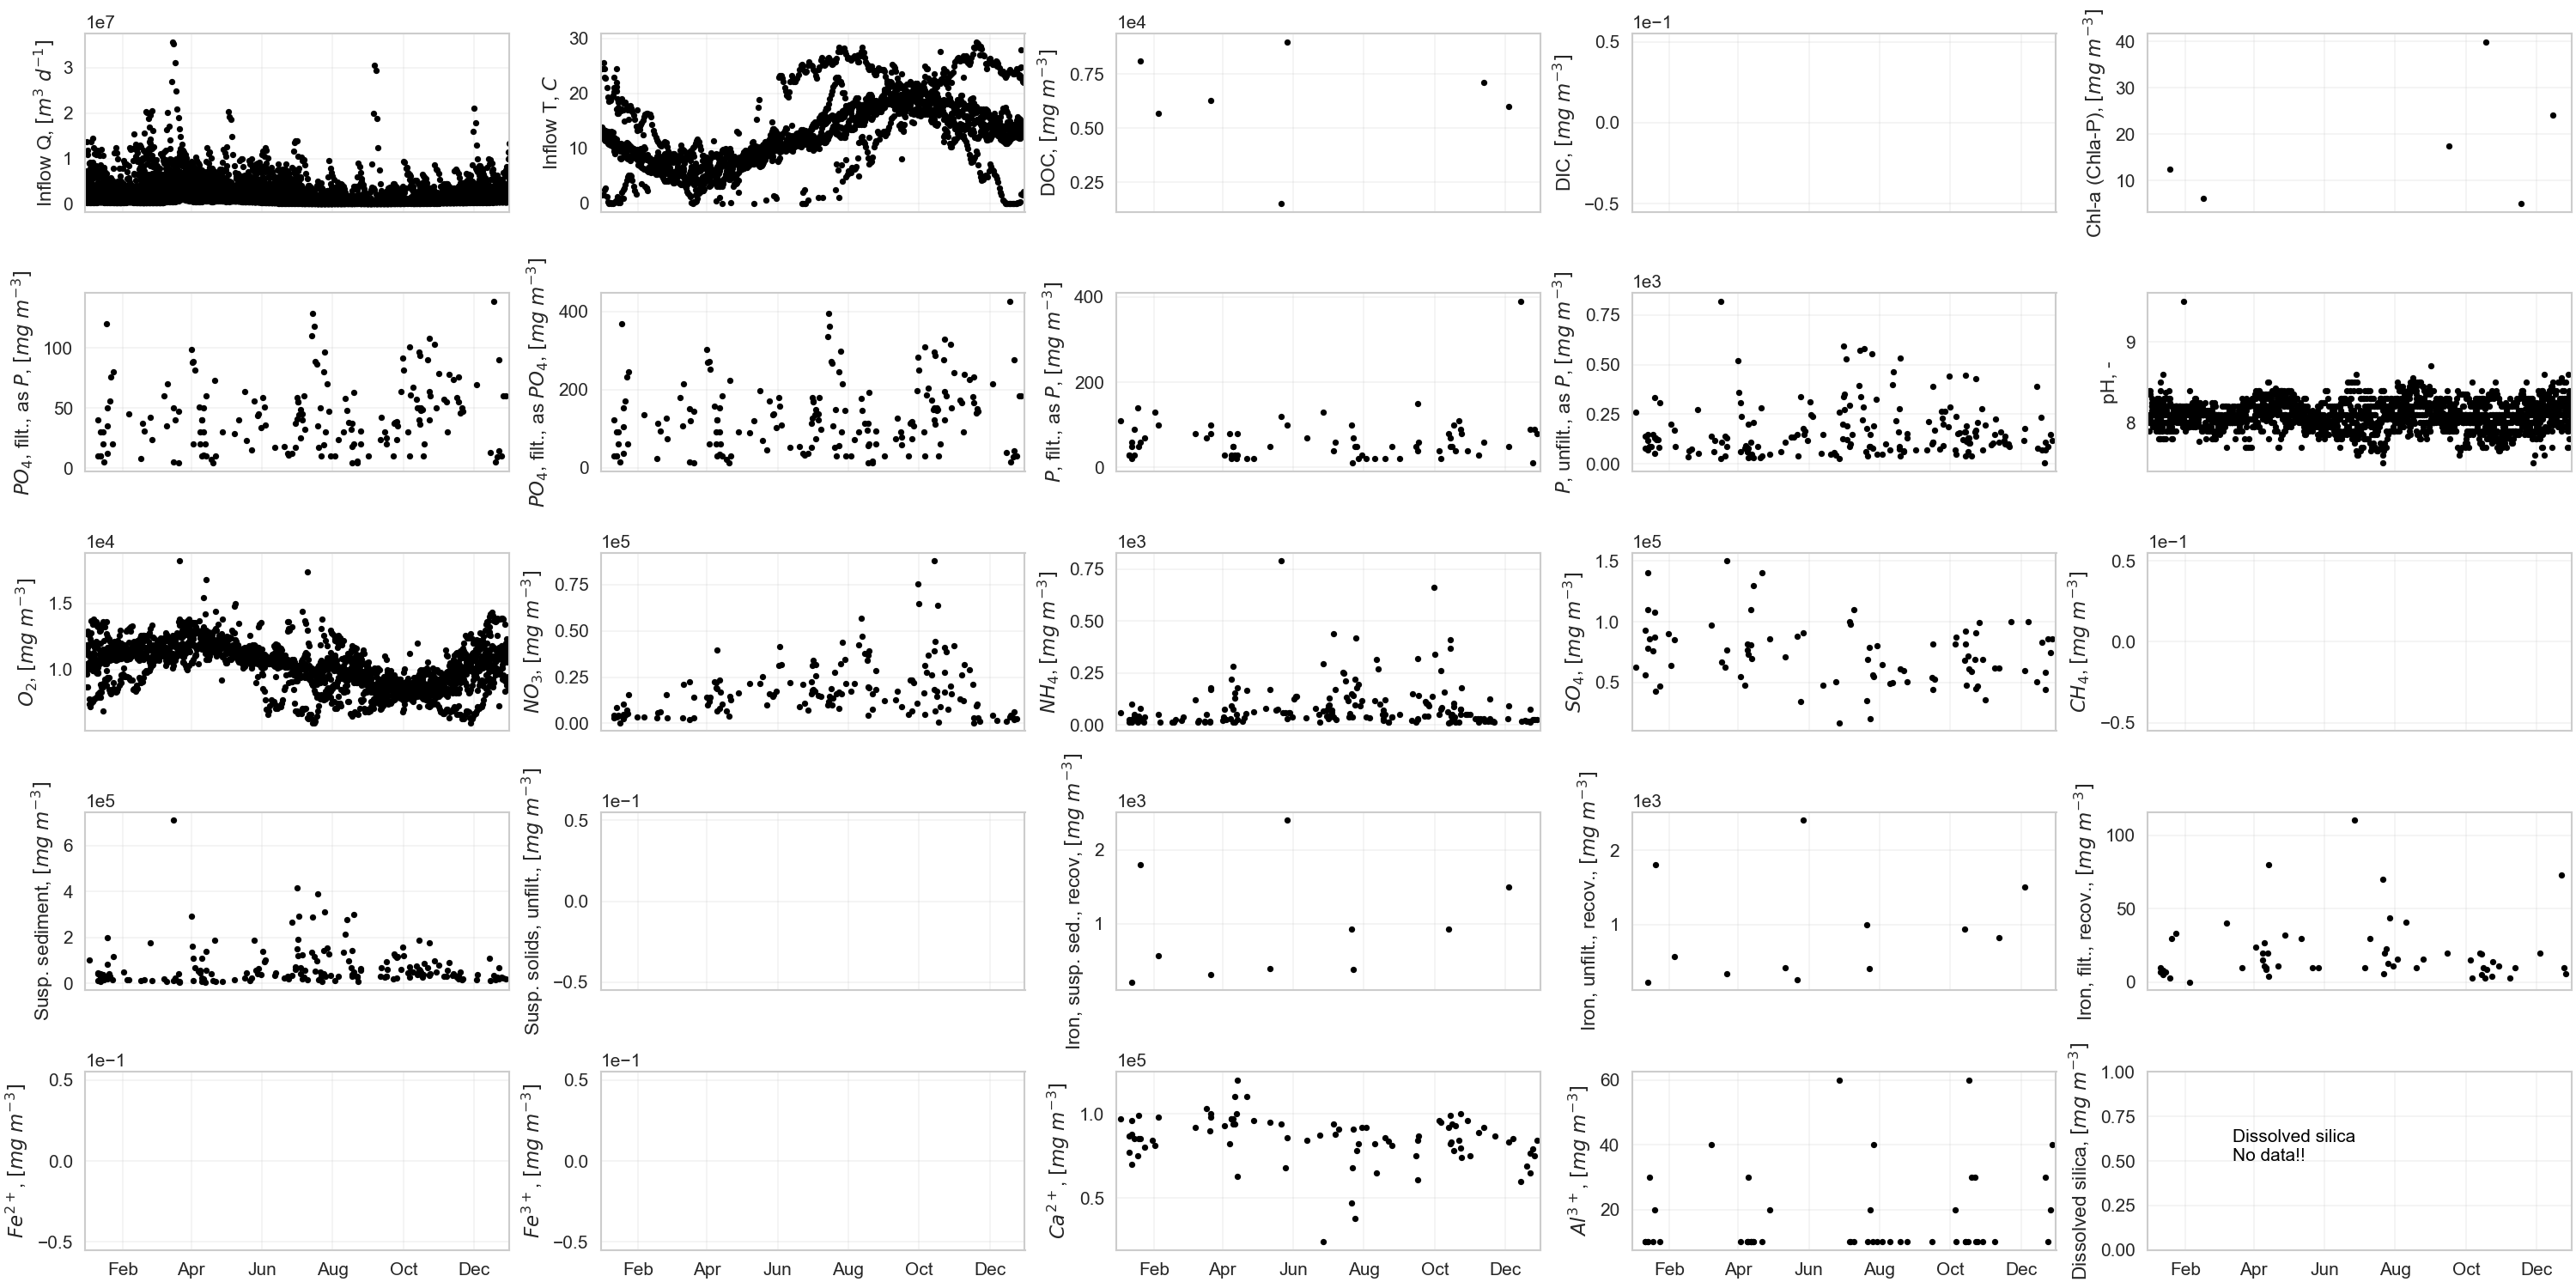
\includegraphics[width=\textwidth]{rivers/Western basin/plot_1yr riverraisin.png}
\end{figure}
\end{frame}


\begin{frame}
\frametitle{Western Basin: Stony creek}
\begin{figure}
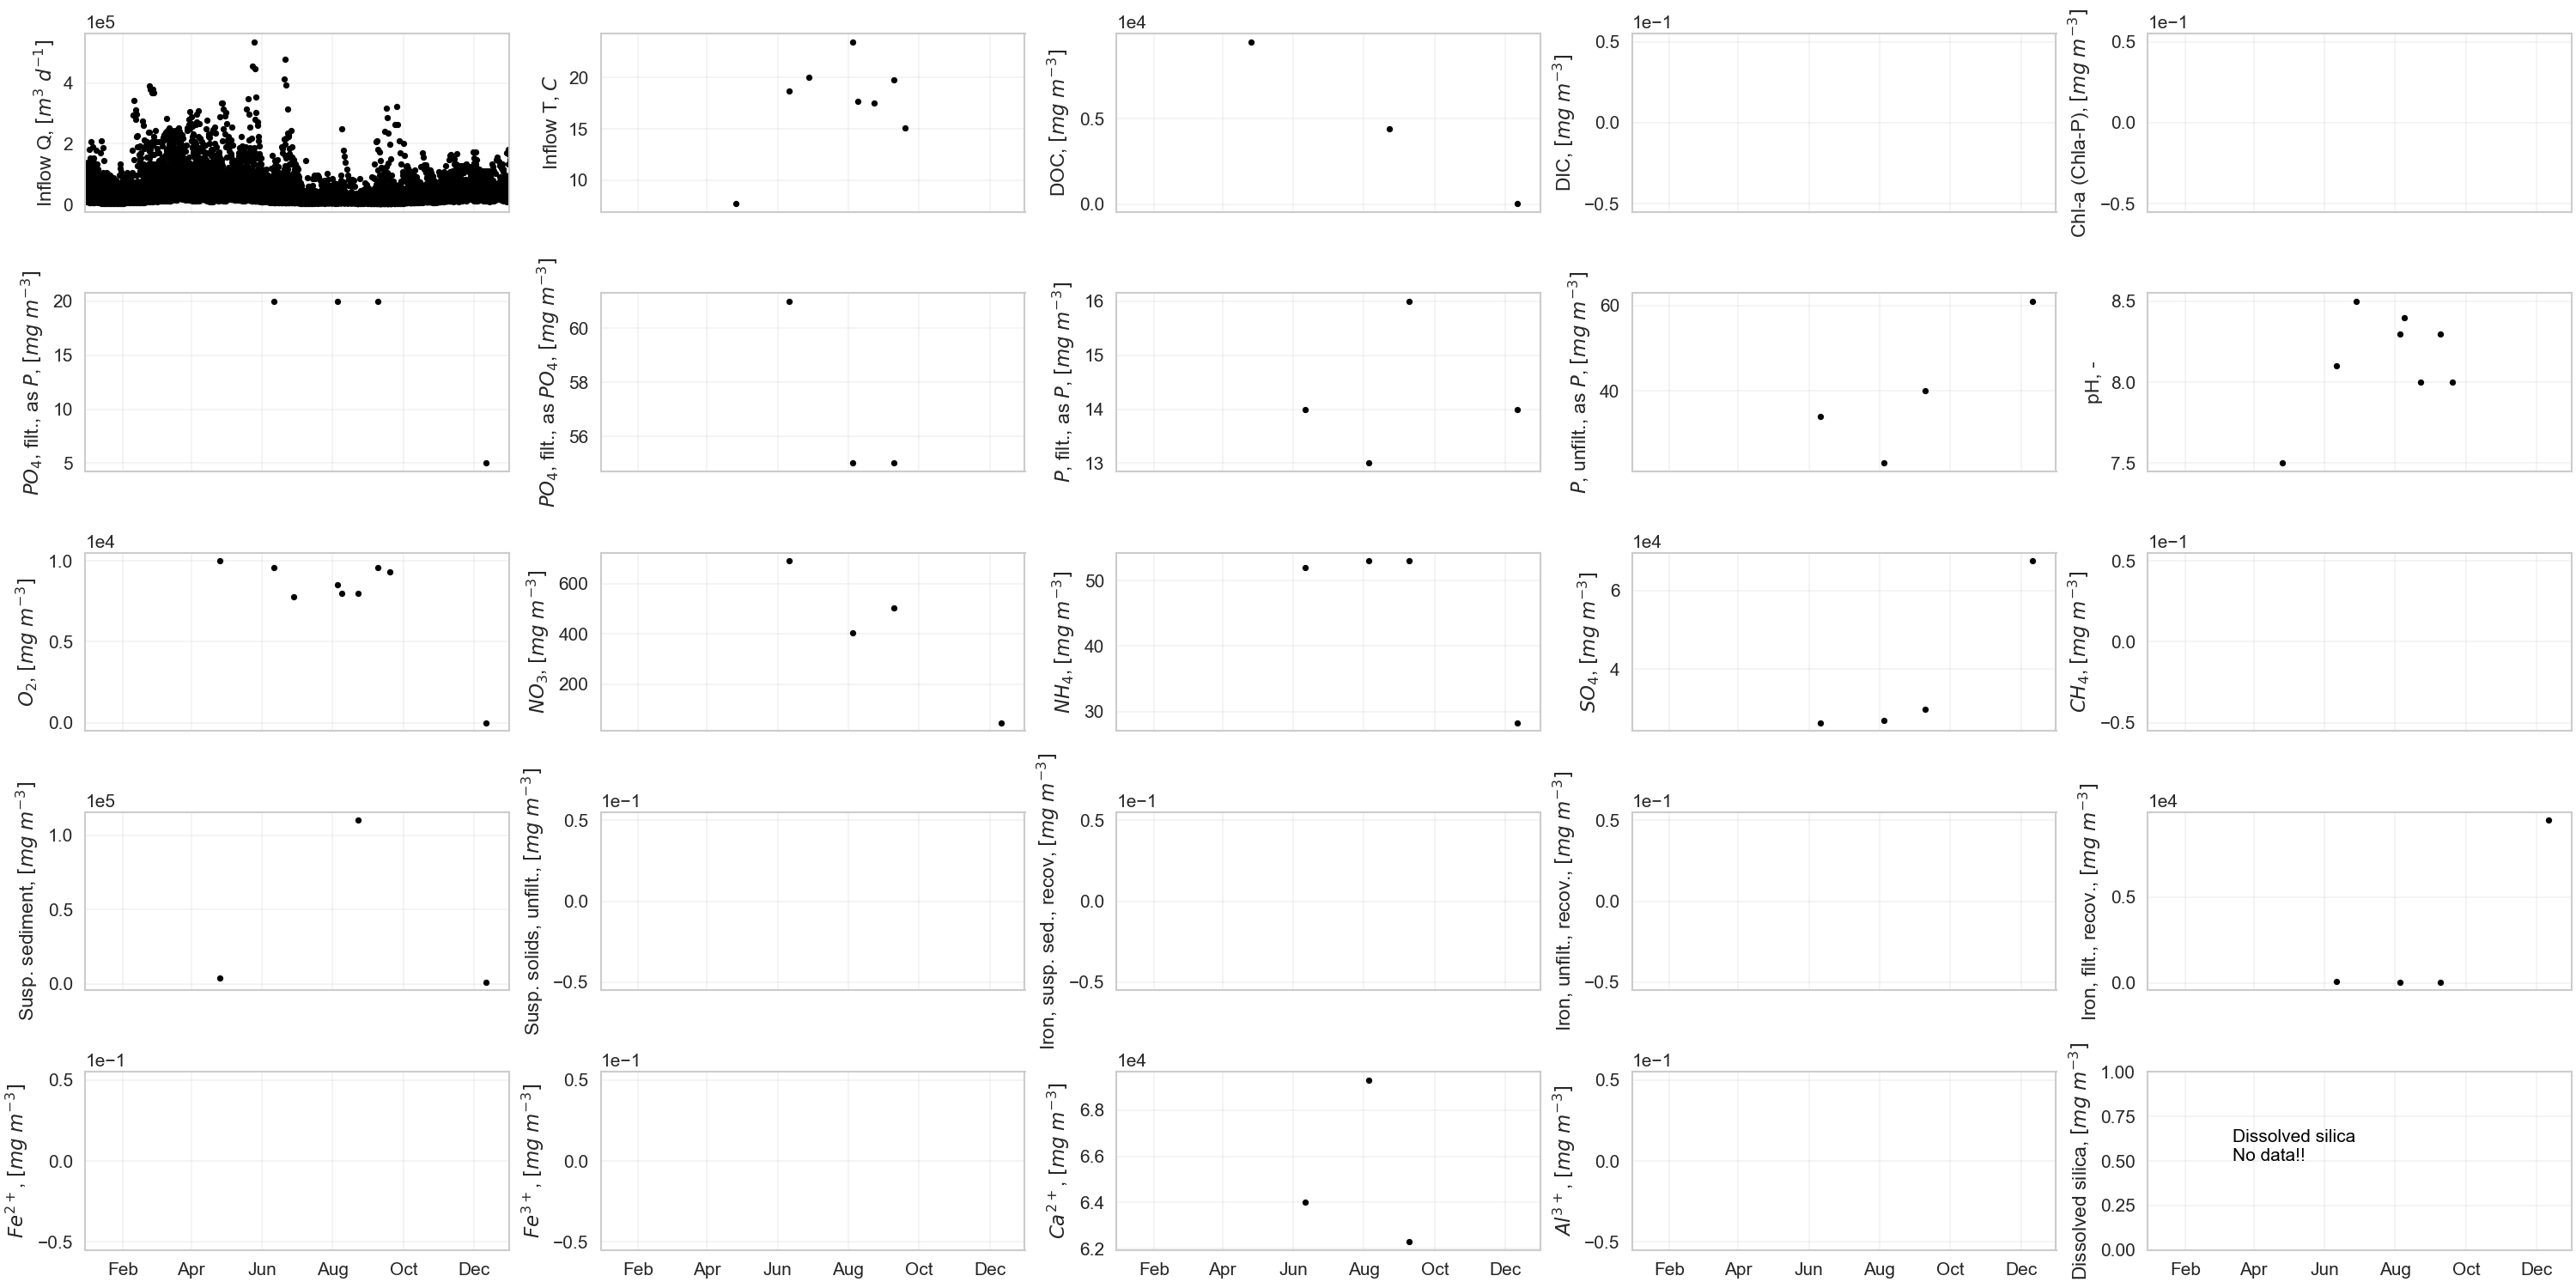
\includegraphics[width=\textwidth]{rivers/Western basin/plot_1yr stonycreek.png}
\end{figure}
\end{frame}


\begin{frame}
\frametitle{Western Basin: Swan creek}
\begin{figure}
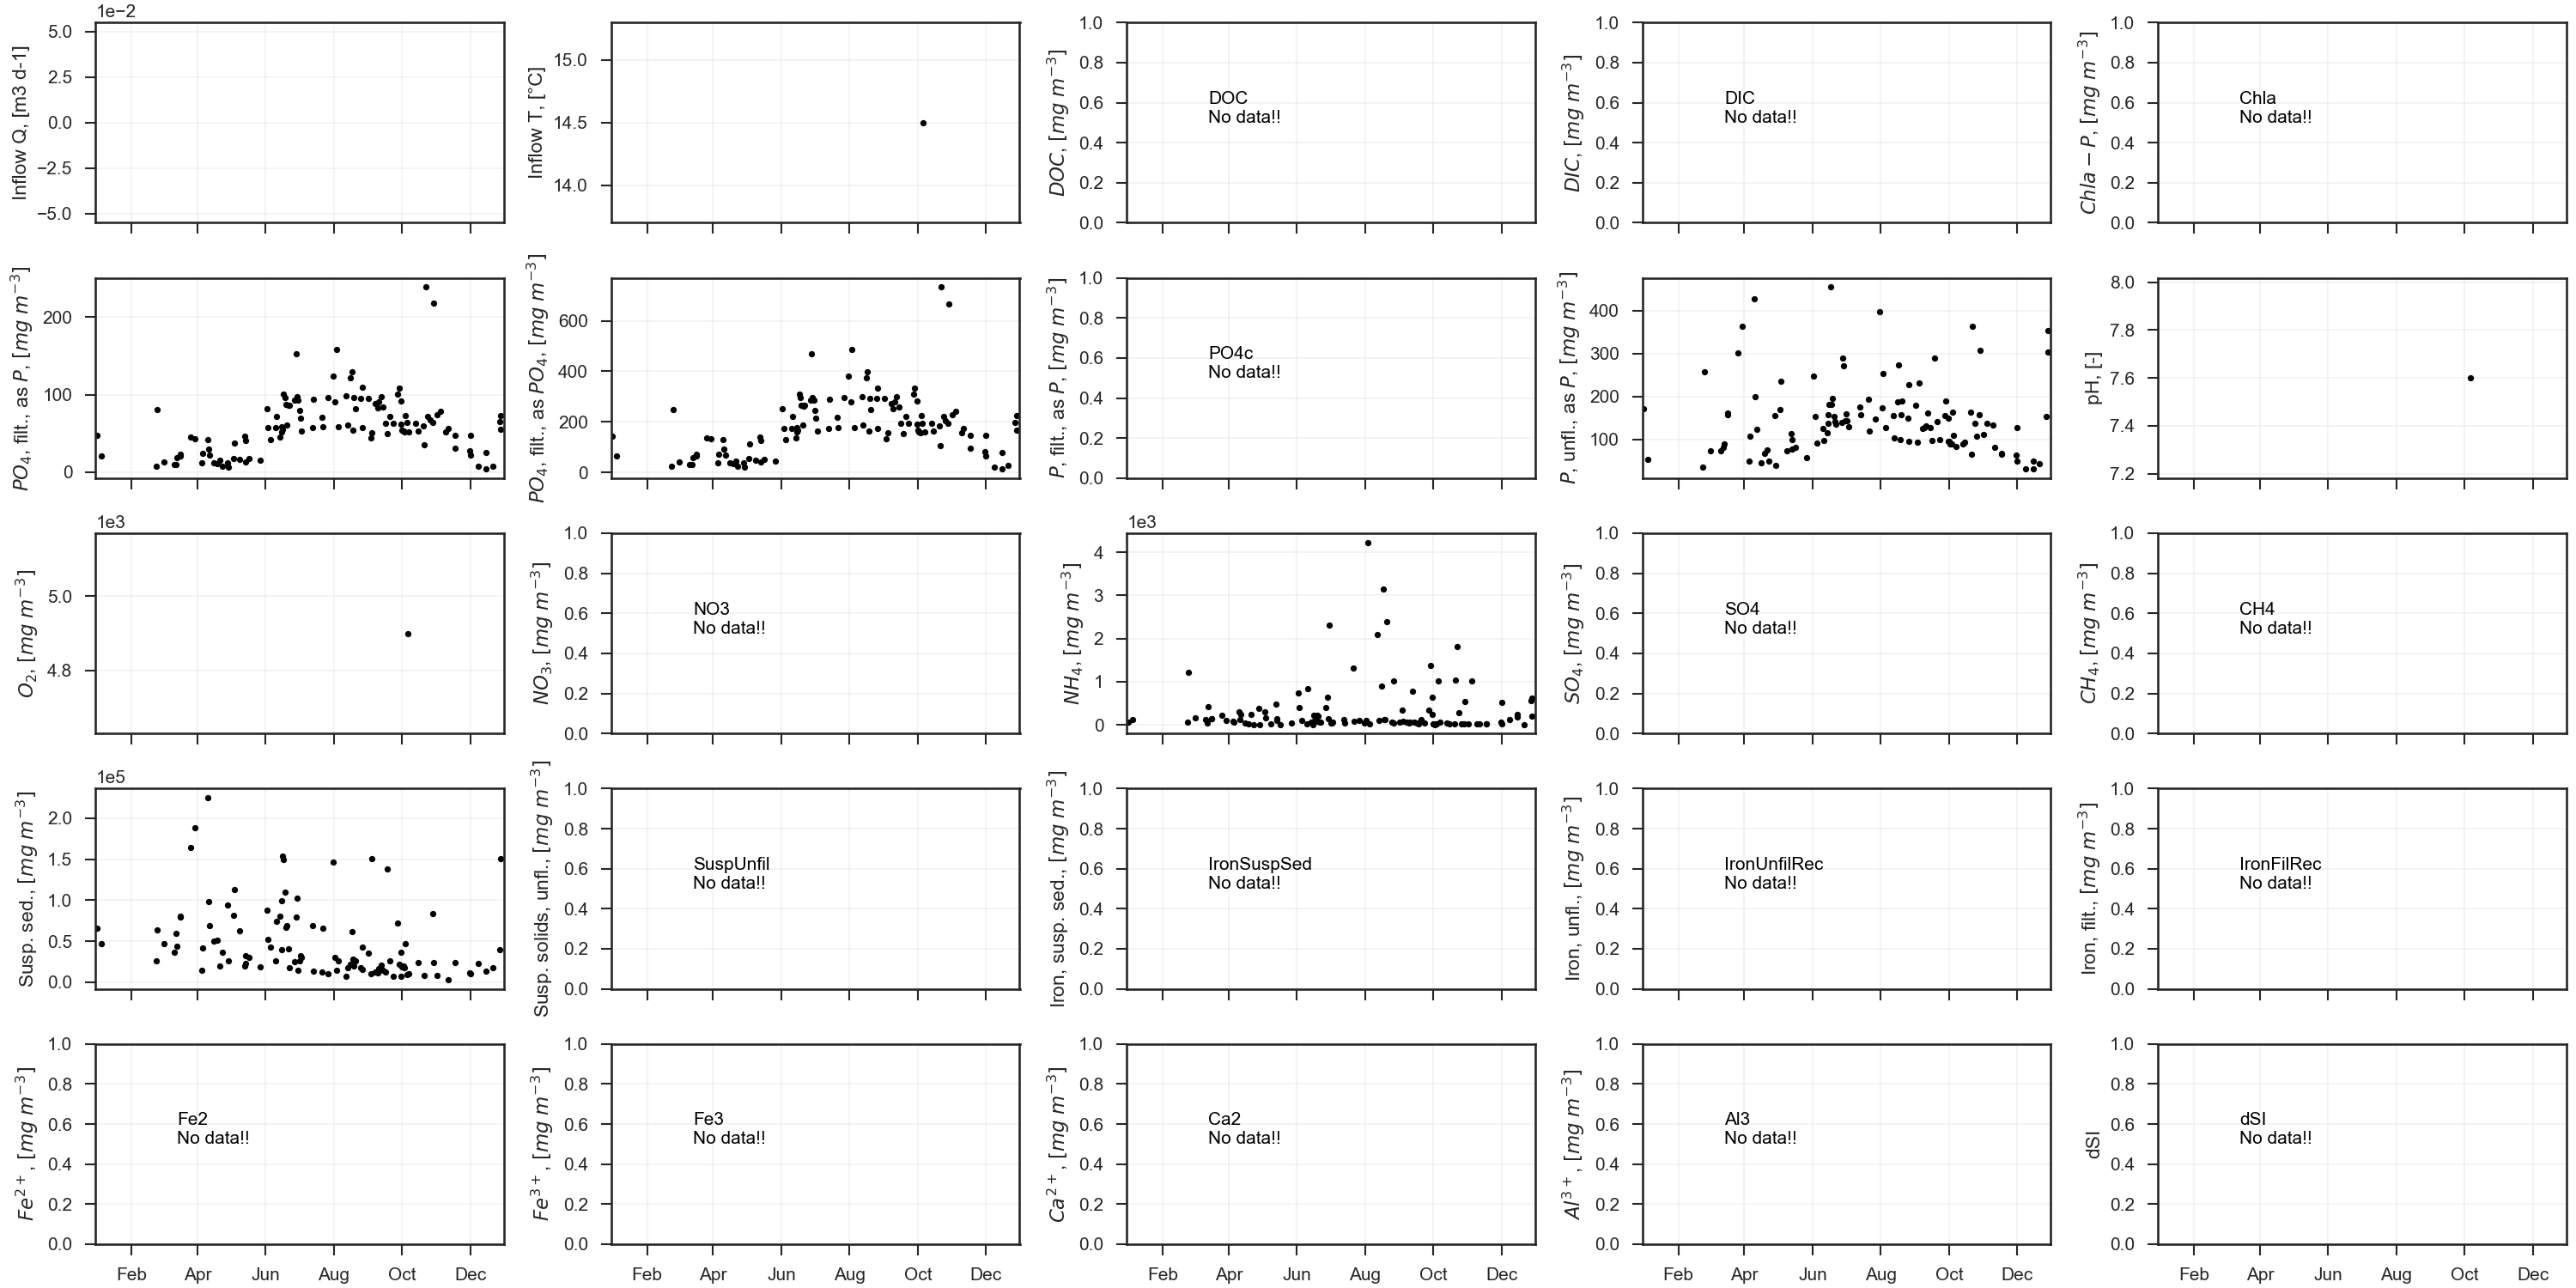
\includegraphics[width=\textwidth]{rivers/Western basin/plot_1yr swancreek.png}
\end{figure}
\end{frame}



\subsection{Central Basin}
\label{sub:central_basin}


\begin{frame}
\frametitle{Central Basin: Ashtabula river}
\begin{figure}
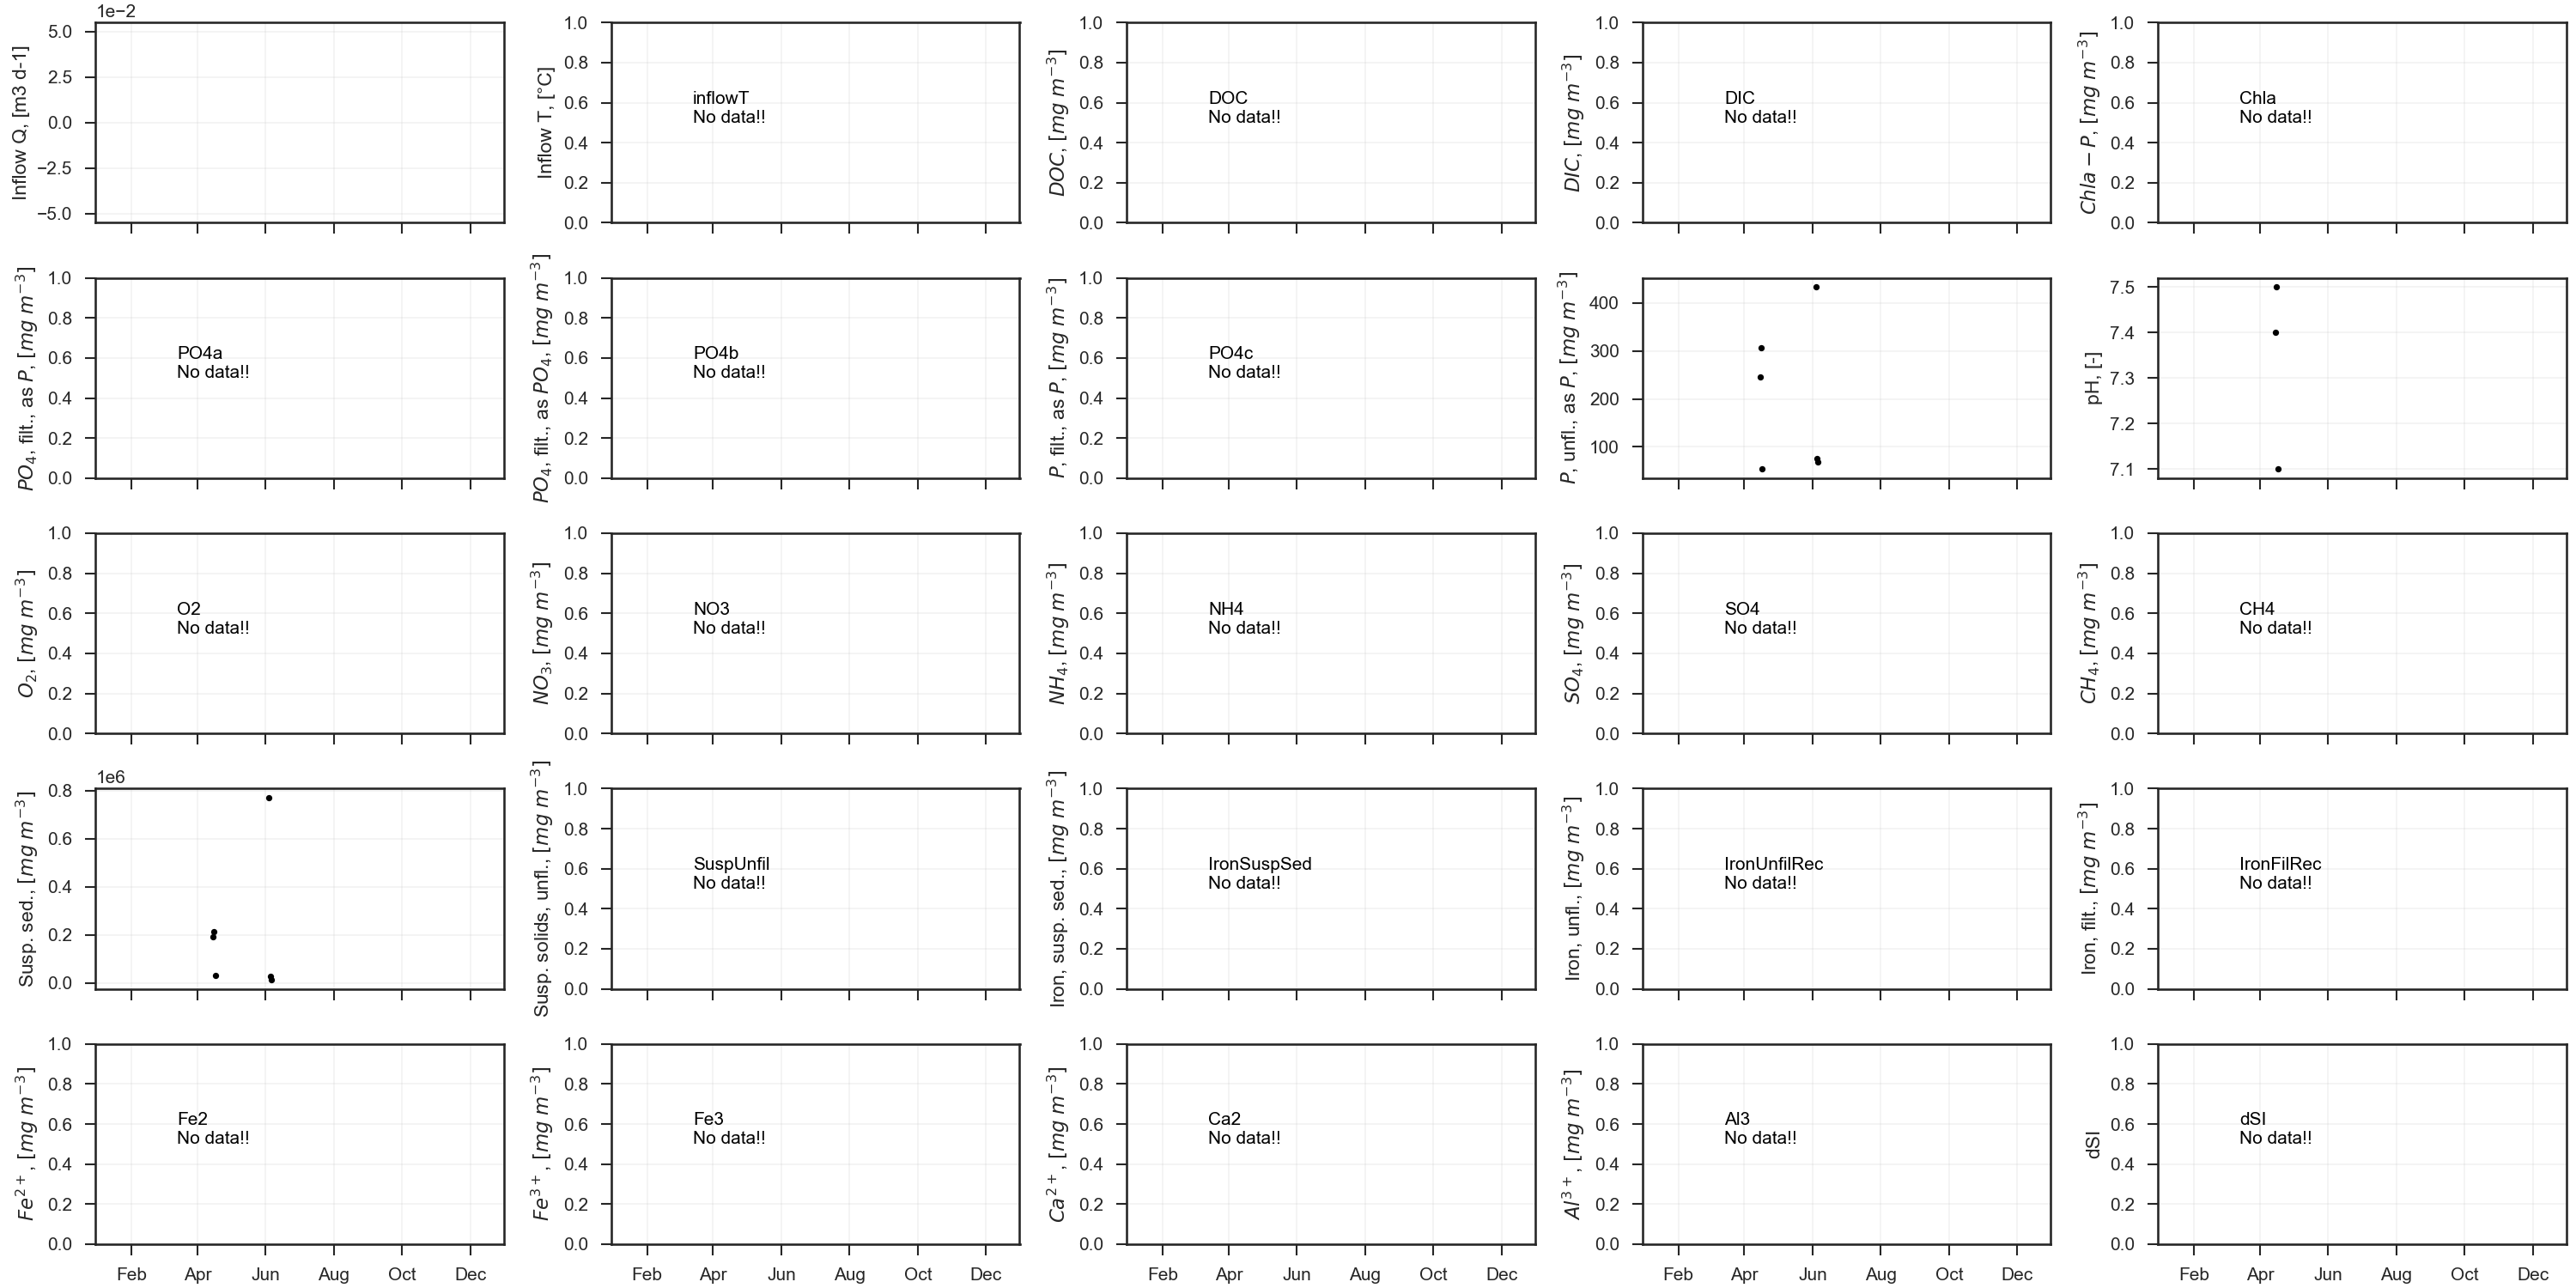
\includegraphics[width=\textwidth]{rivers/Central basin/plot_1yr ashtabulariver.png}
\end{figure}
\end{frame}

\begin{frame}
\frametitle{Central Basin: Black river}
\begin{figure}
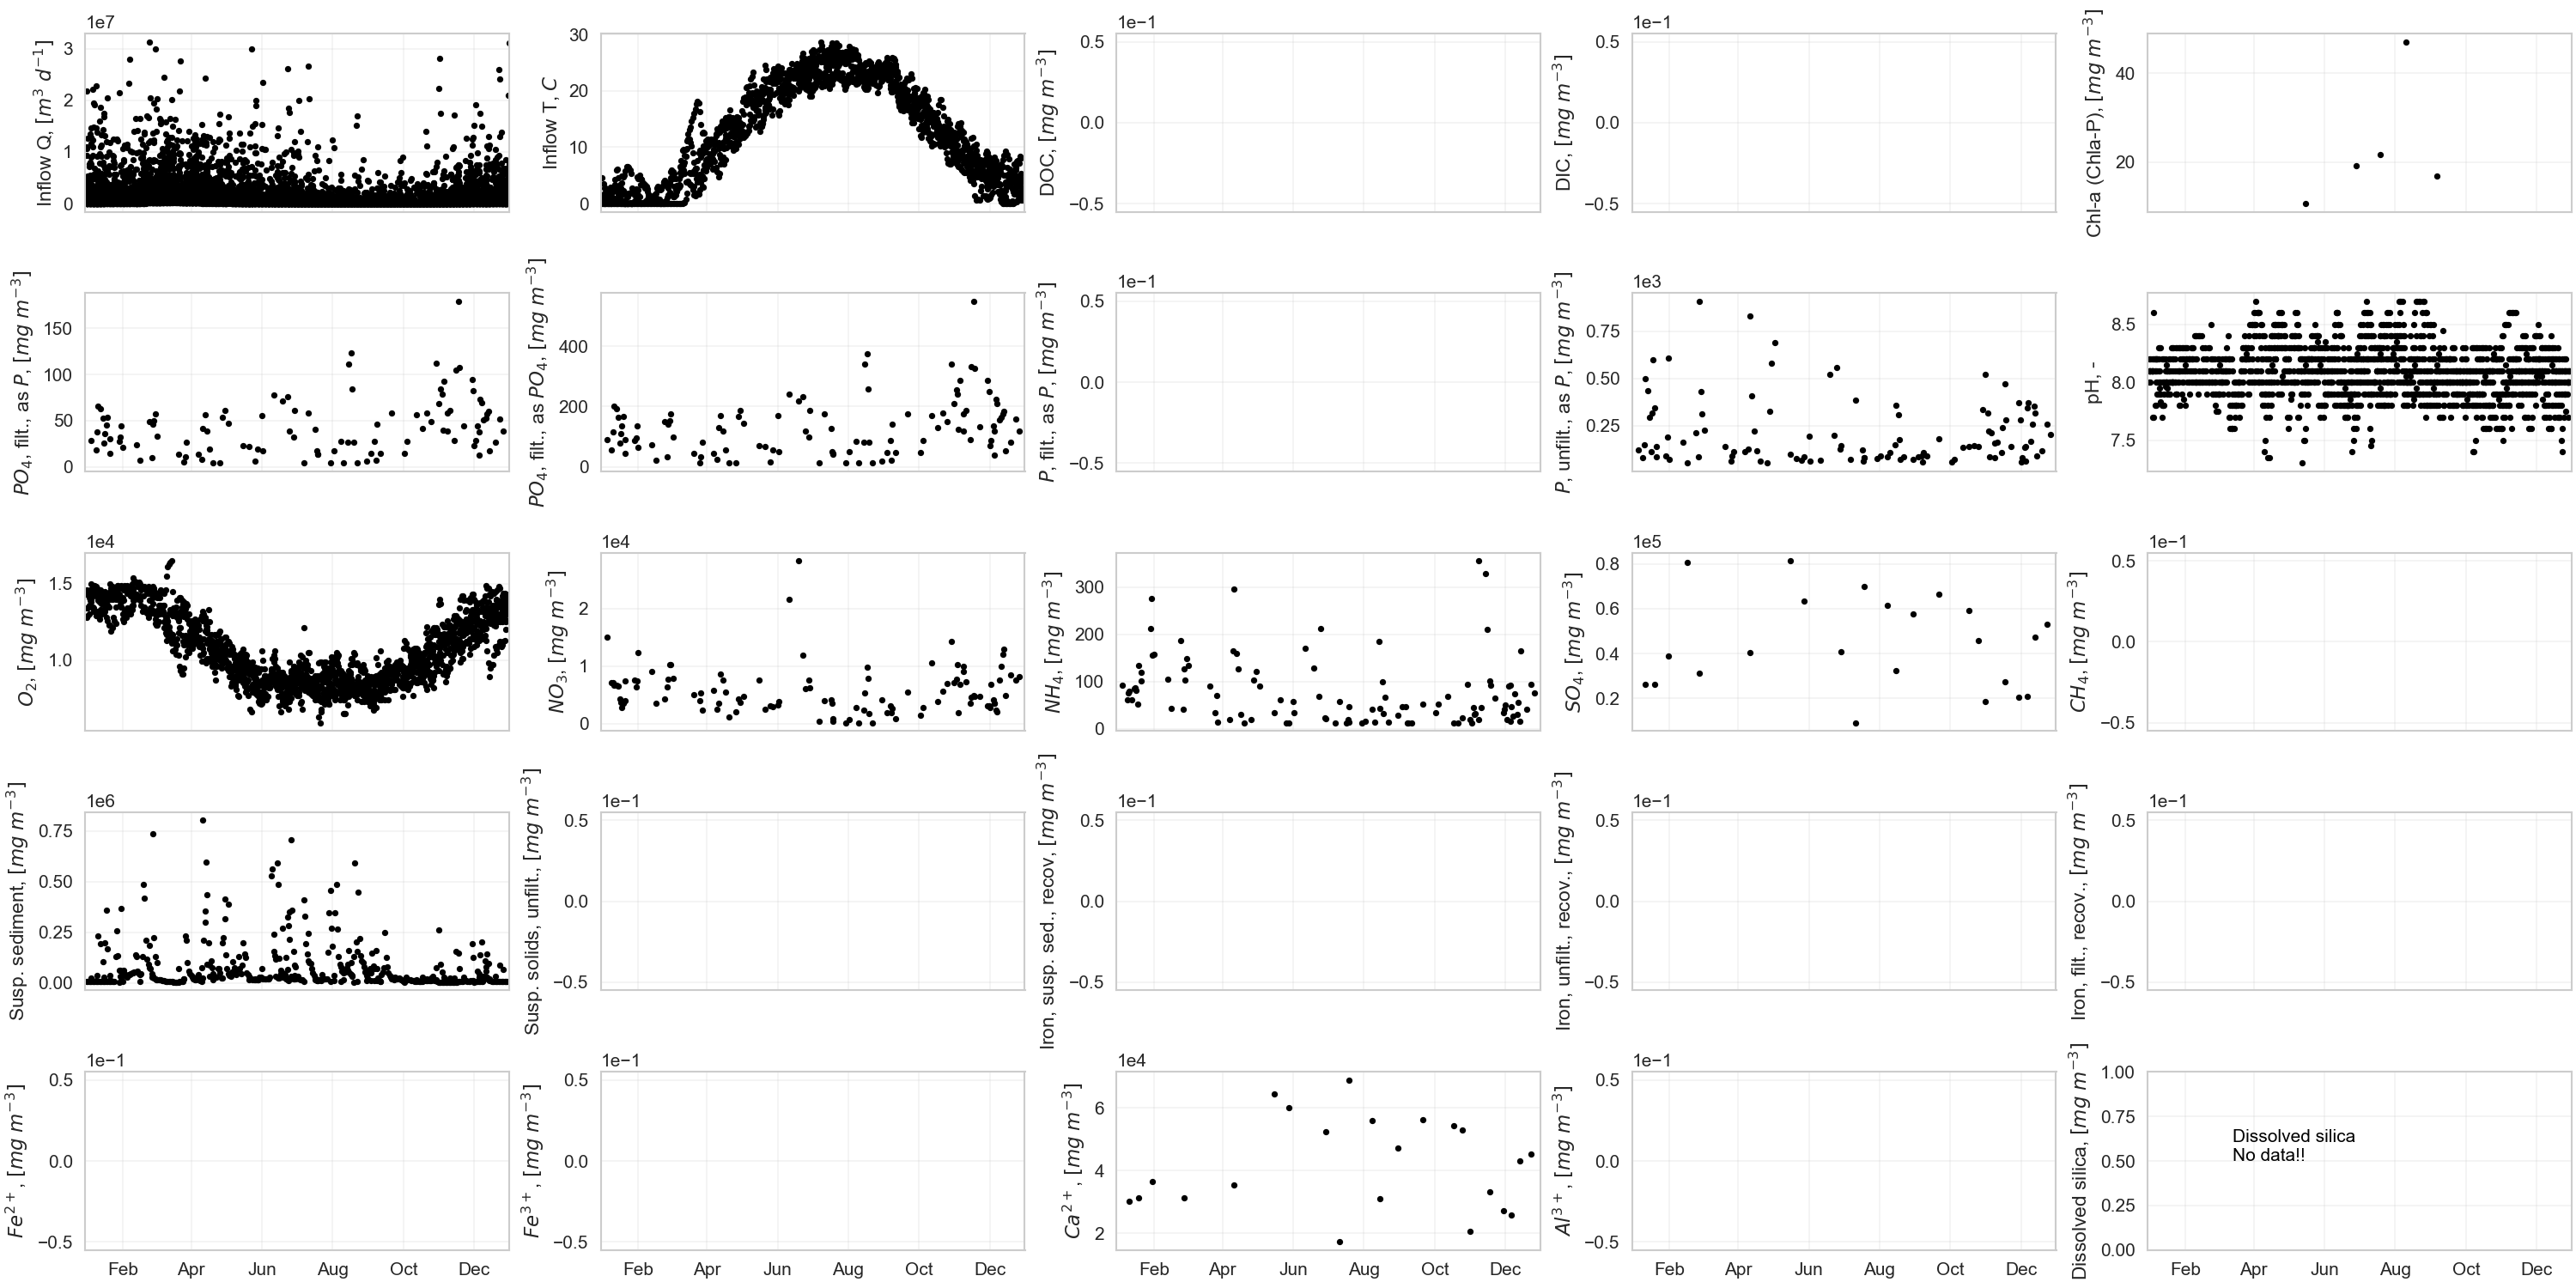
\includegraphics[width=\textwidth]{rivers/Central basin/plot_1yr blackriver.png}
\end{figure}
\end{frame}

\begin{frame}
\frametitle{Central Basin: Chagrin river}
\begin{figure}
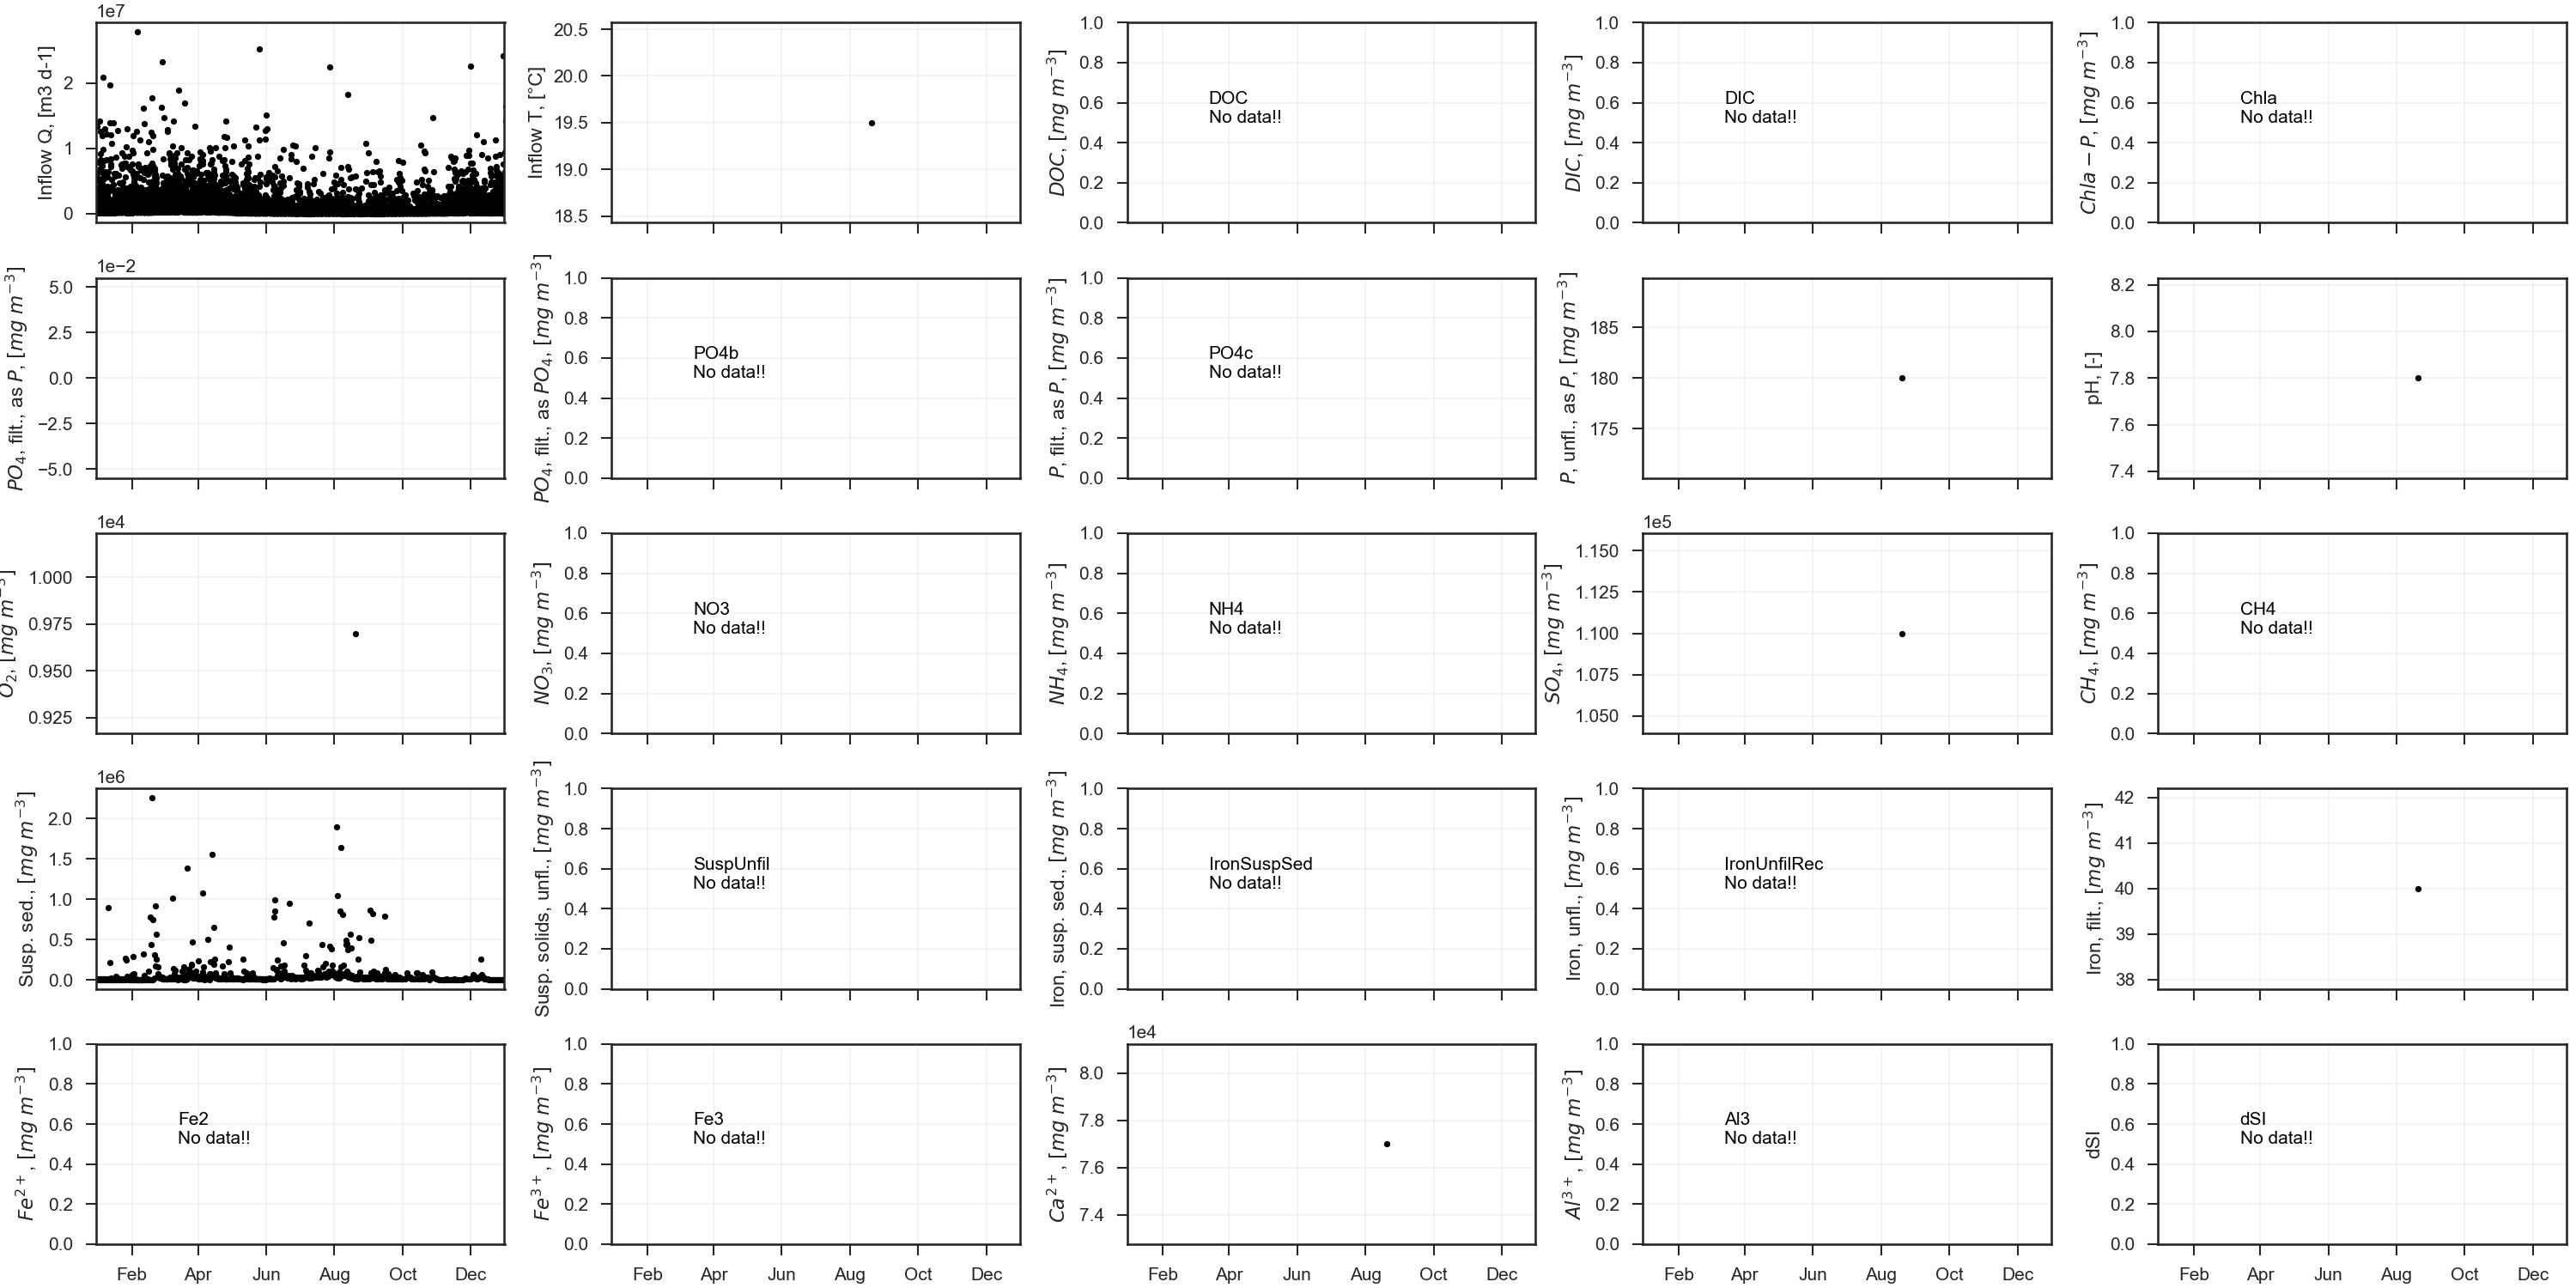
\includegraphics[width=\textwidth]{rivers/Central basin/plot_1yr chagrinriver.png}
\end{figure}
\end{frame}

\begin{frame}
\frametitle{Central Basin: Conneaut creek}
\begin{figure}
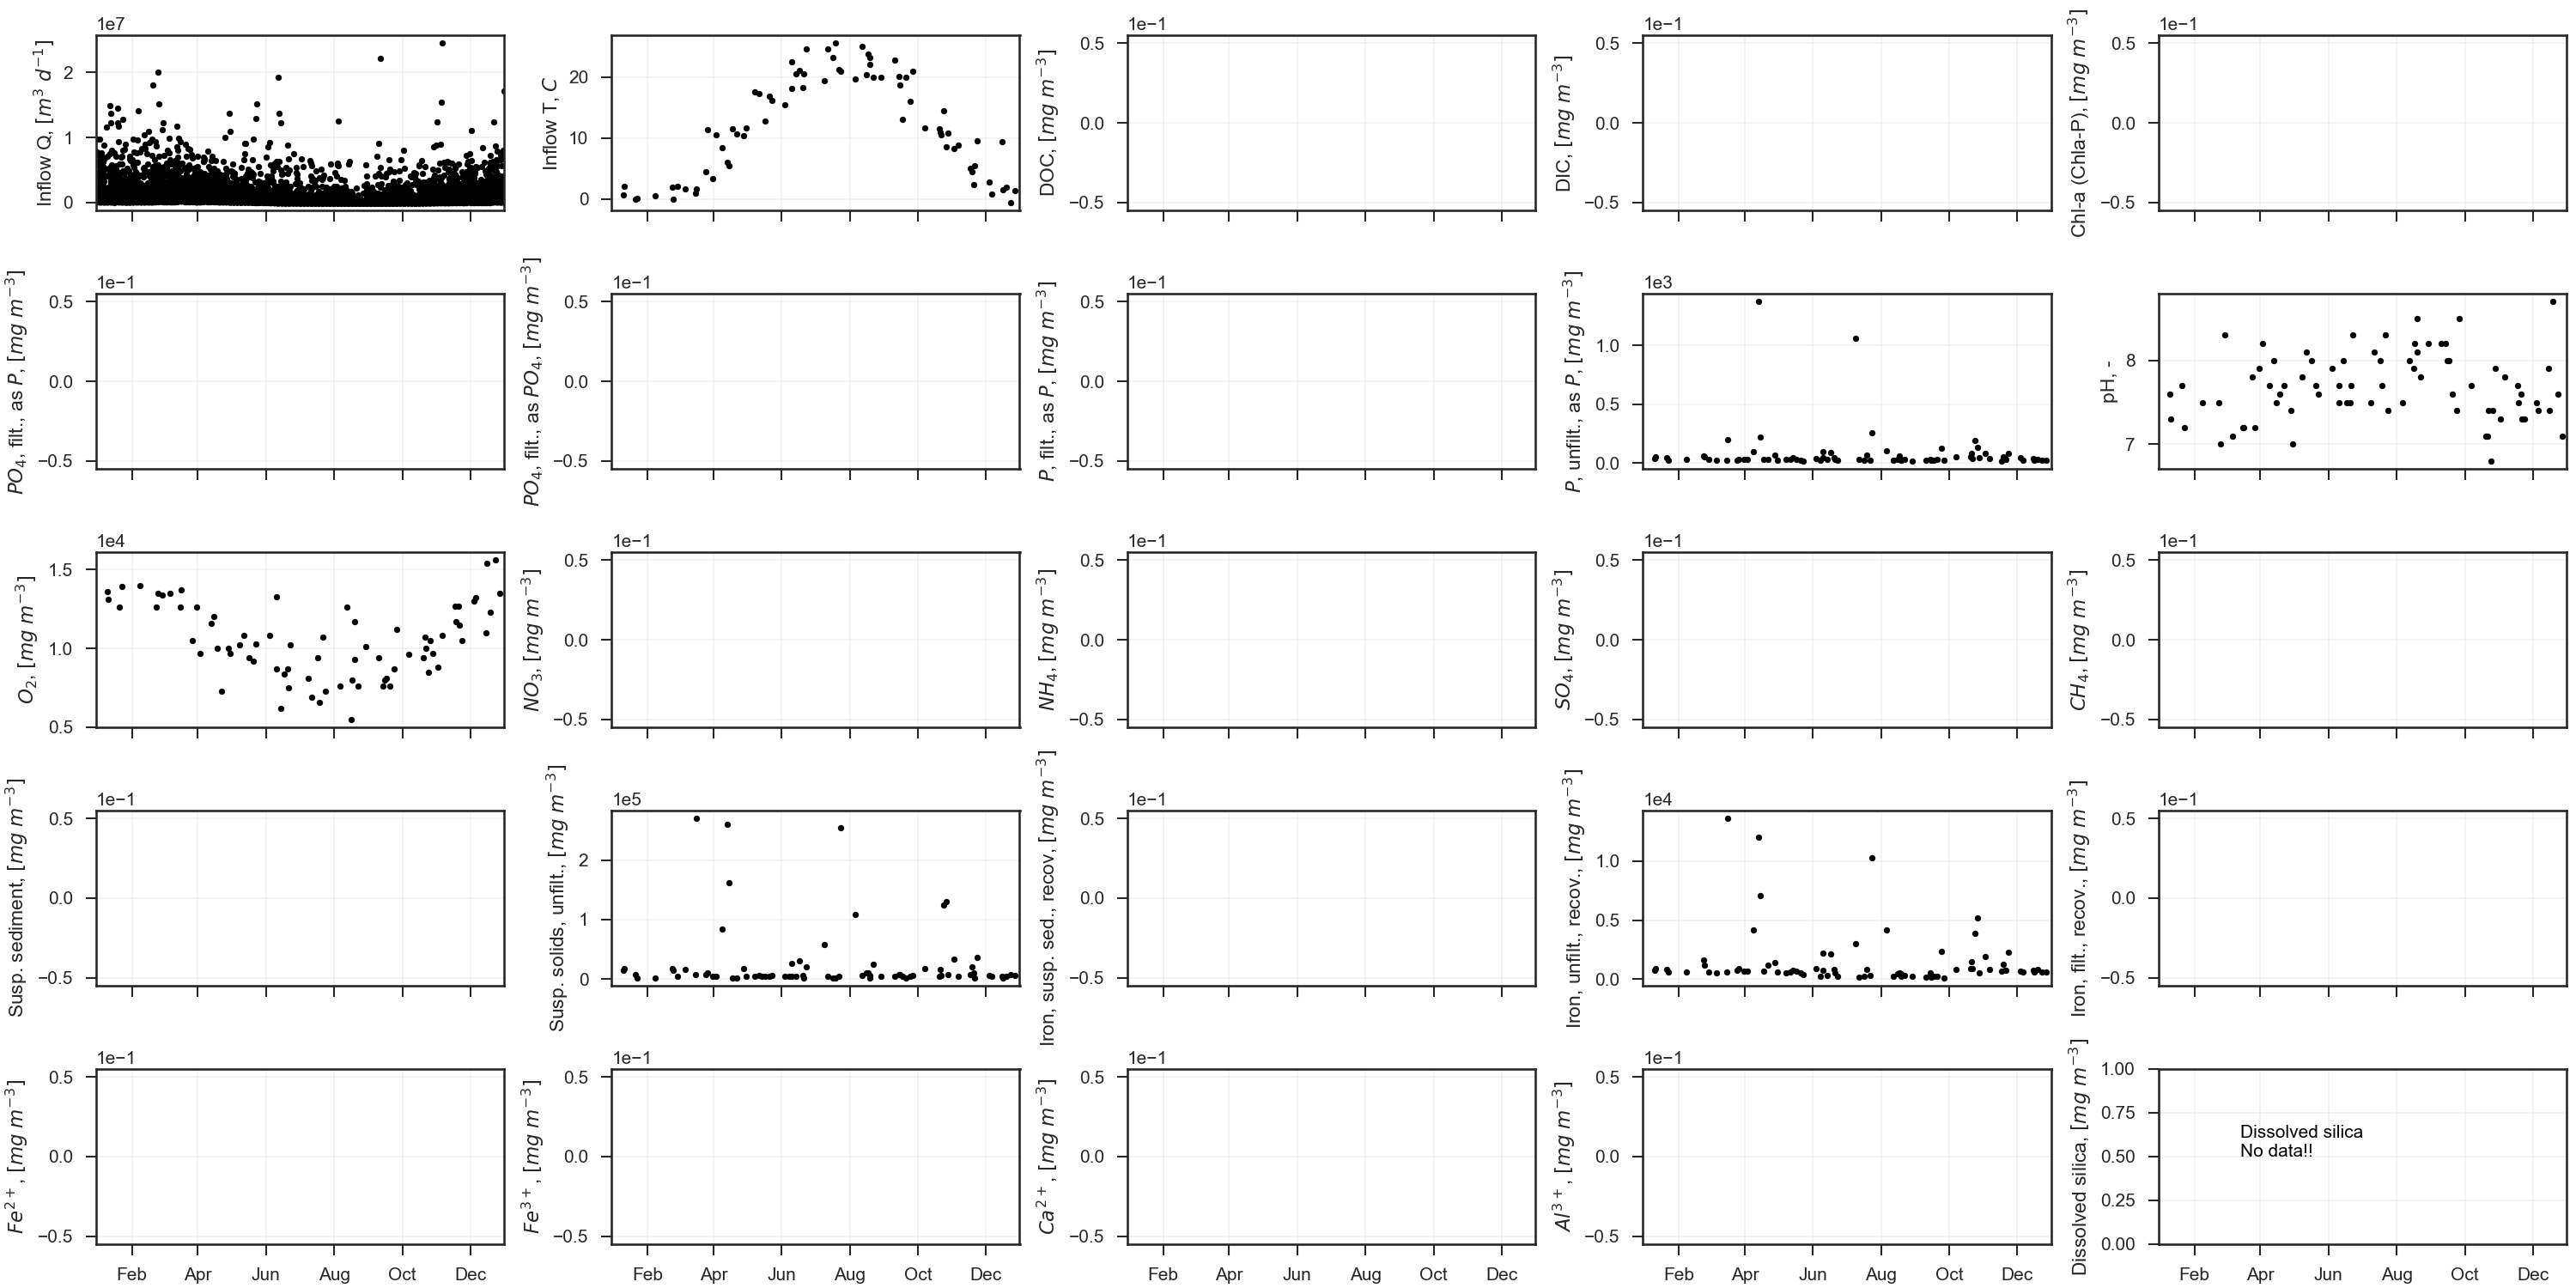
\includegraphics[width=\textwidth]{rivers/Central basin/plot_1yr conneautcreek.png}
\end{figure}
\end{frame}

\begin{frame}
\frametitle{Central Basin: Cuyahoga river}
\begin{figure}
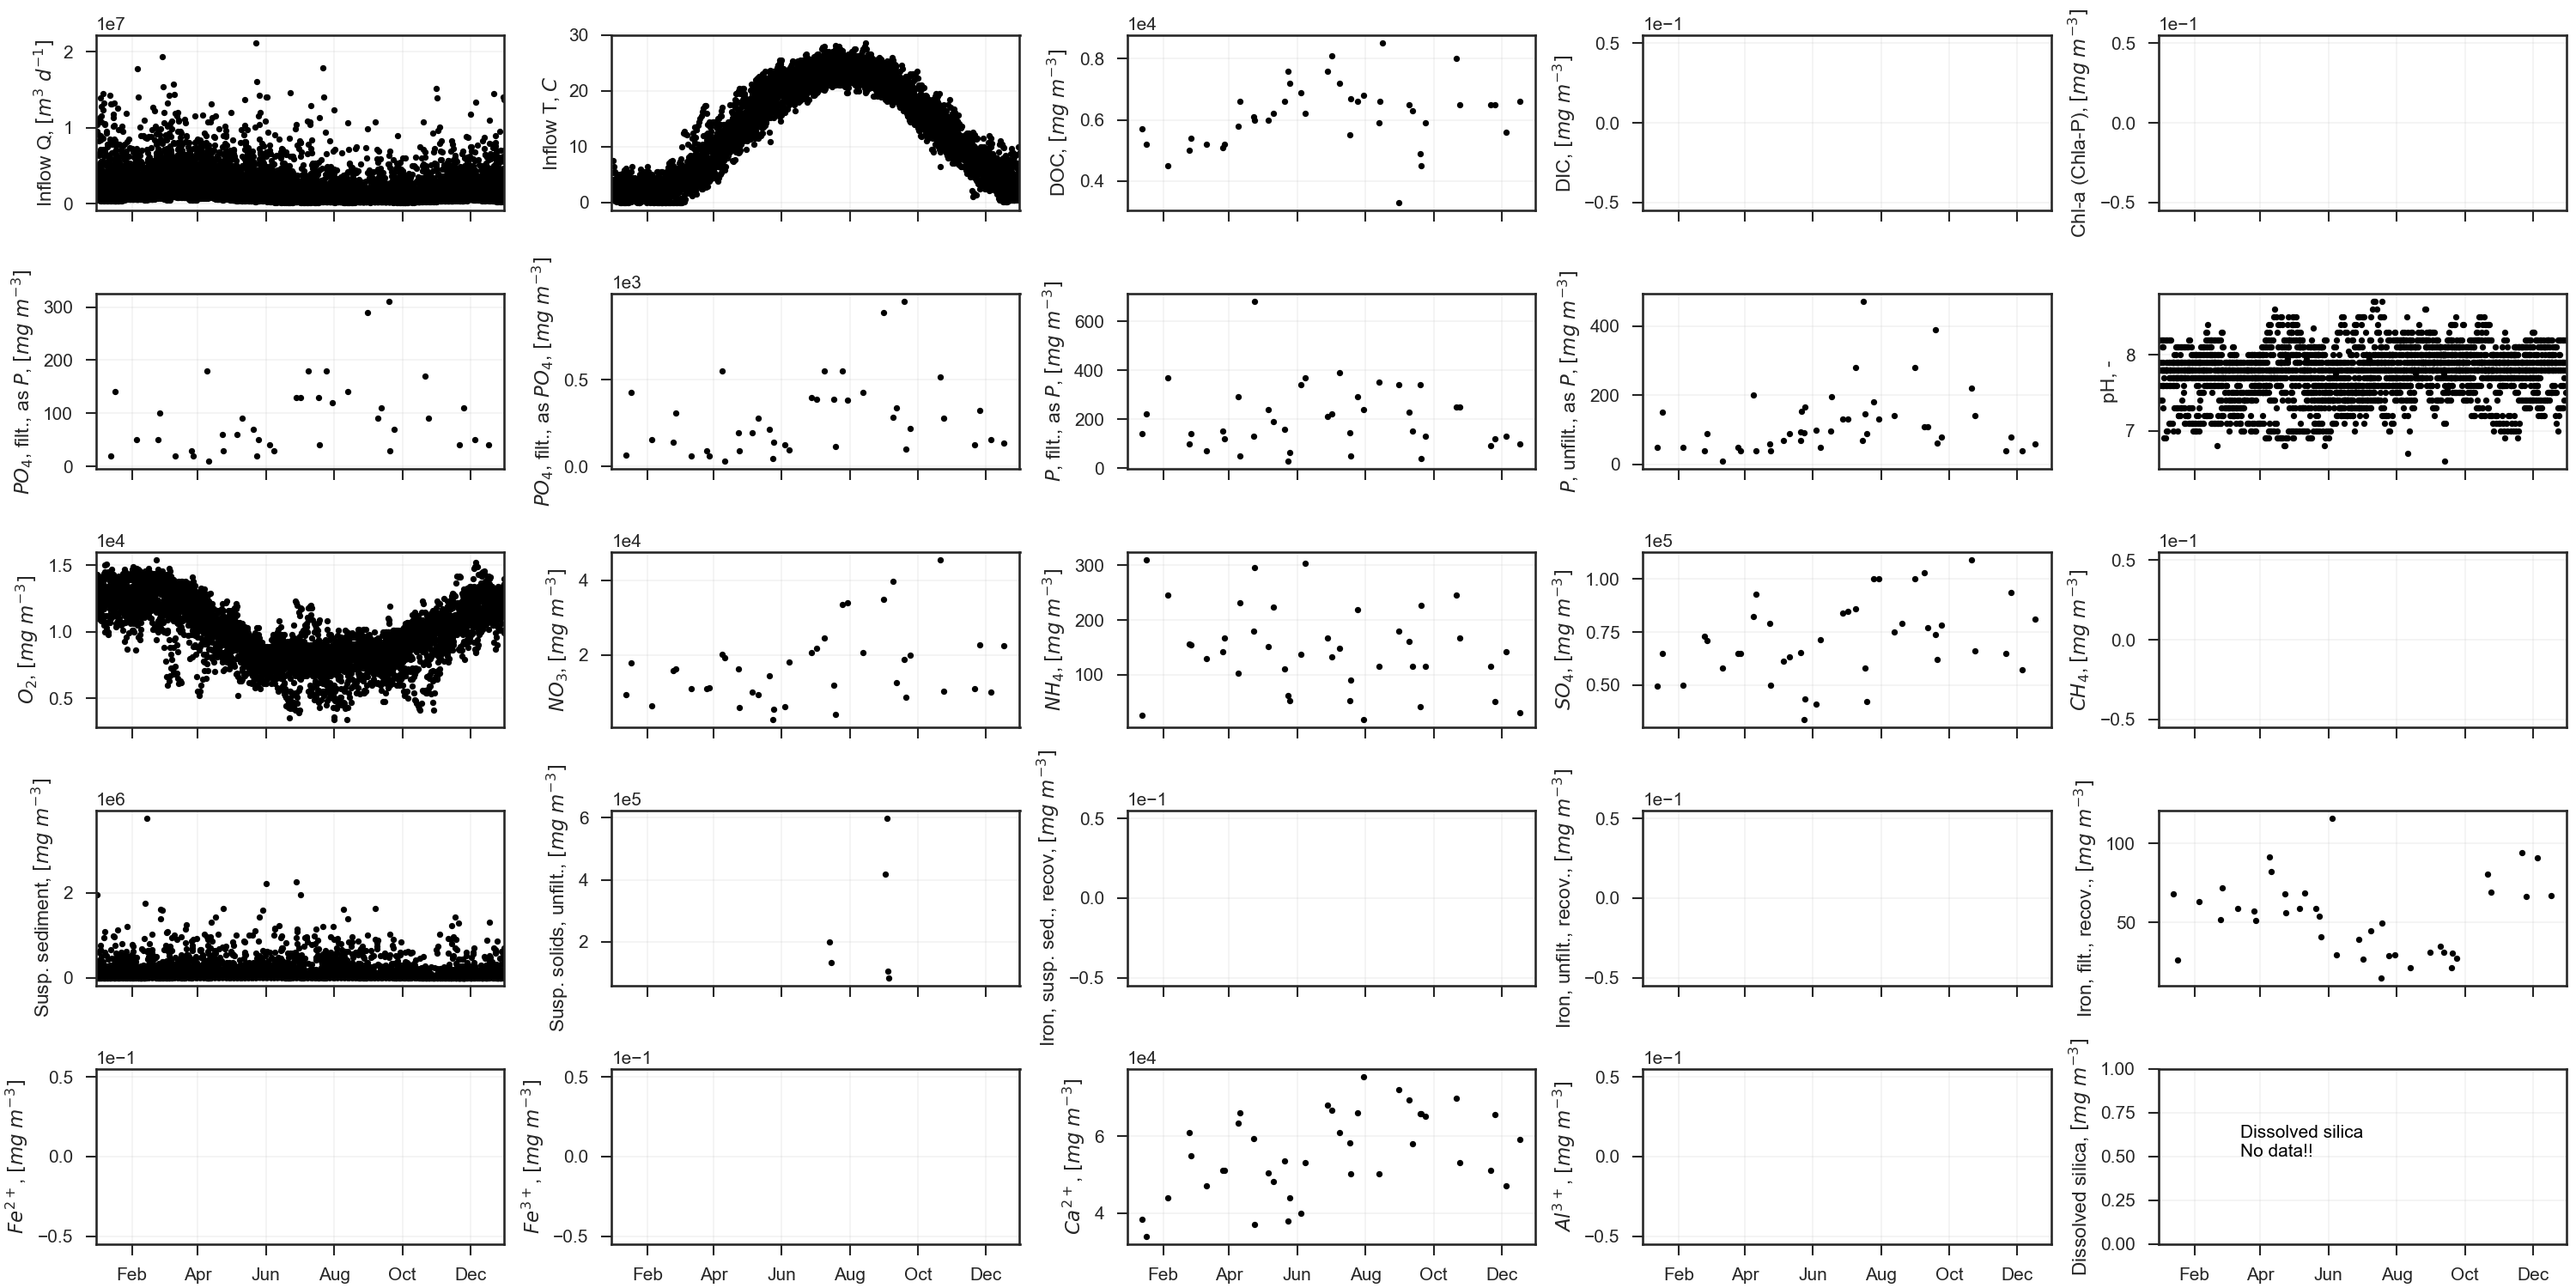
\includegraphics[width=\textwidth]{rivers/Central basin/plot_1yr cuyahogariver.png}
\end{figure}
\end{frame}

\begin{frame}
\frametitle{Central Basin: Grand river}
\begin{figure}
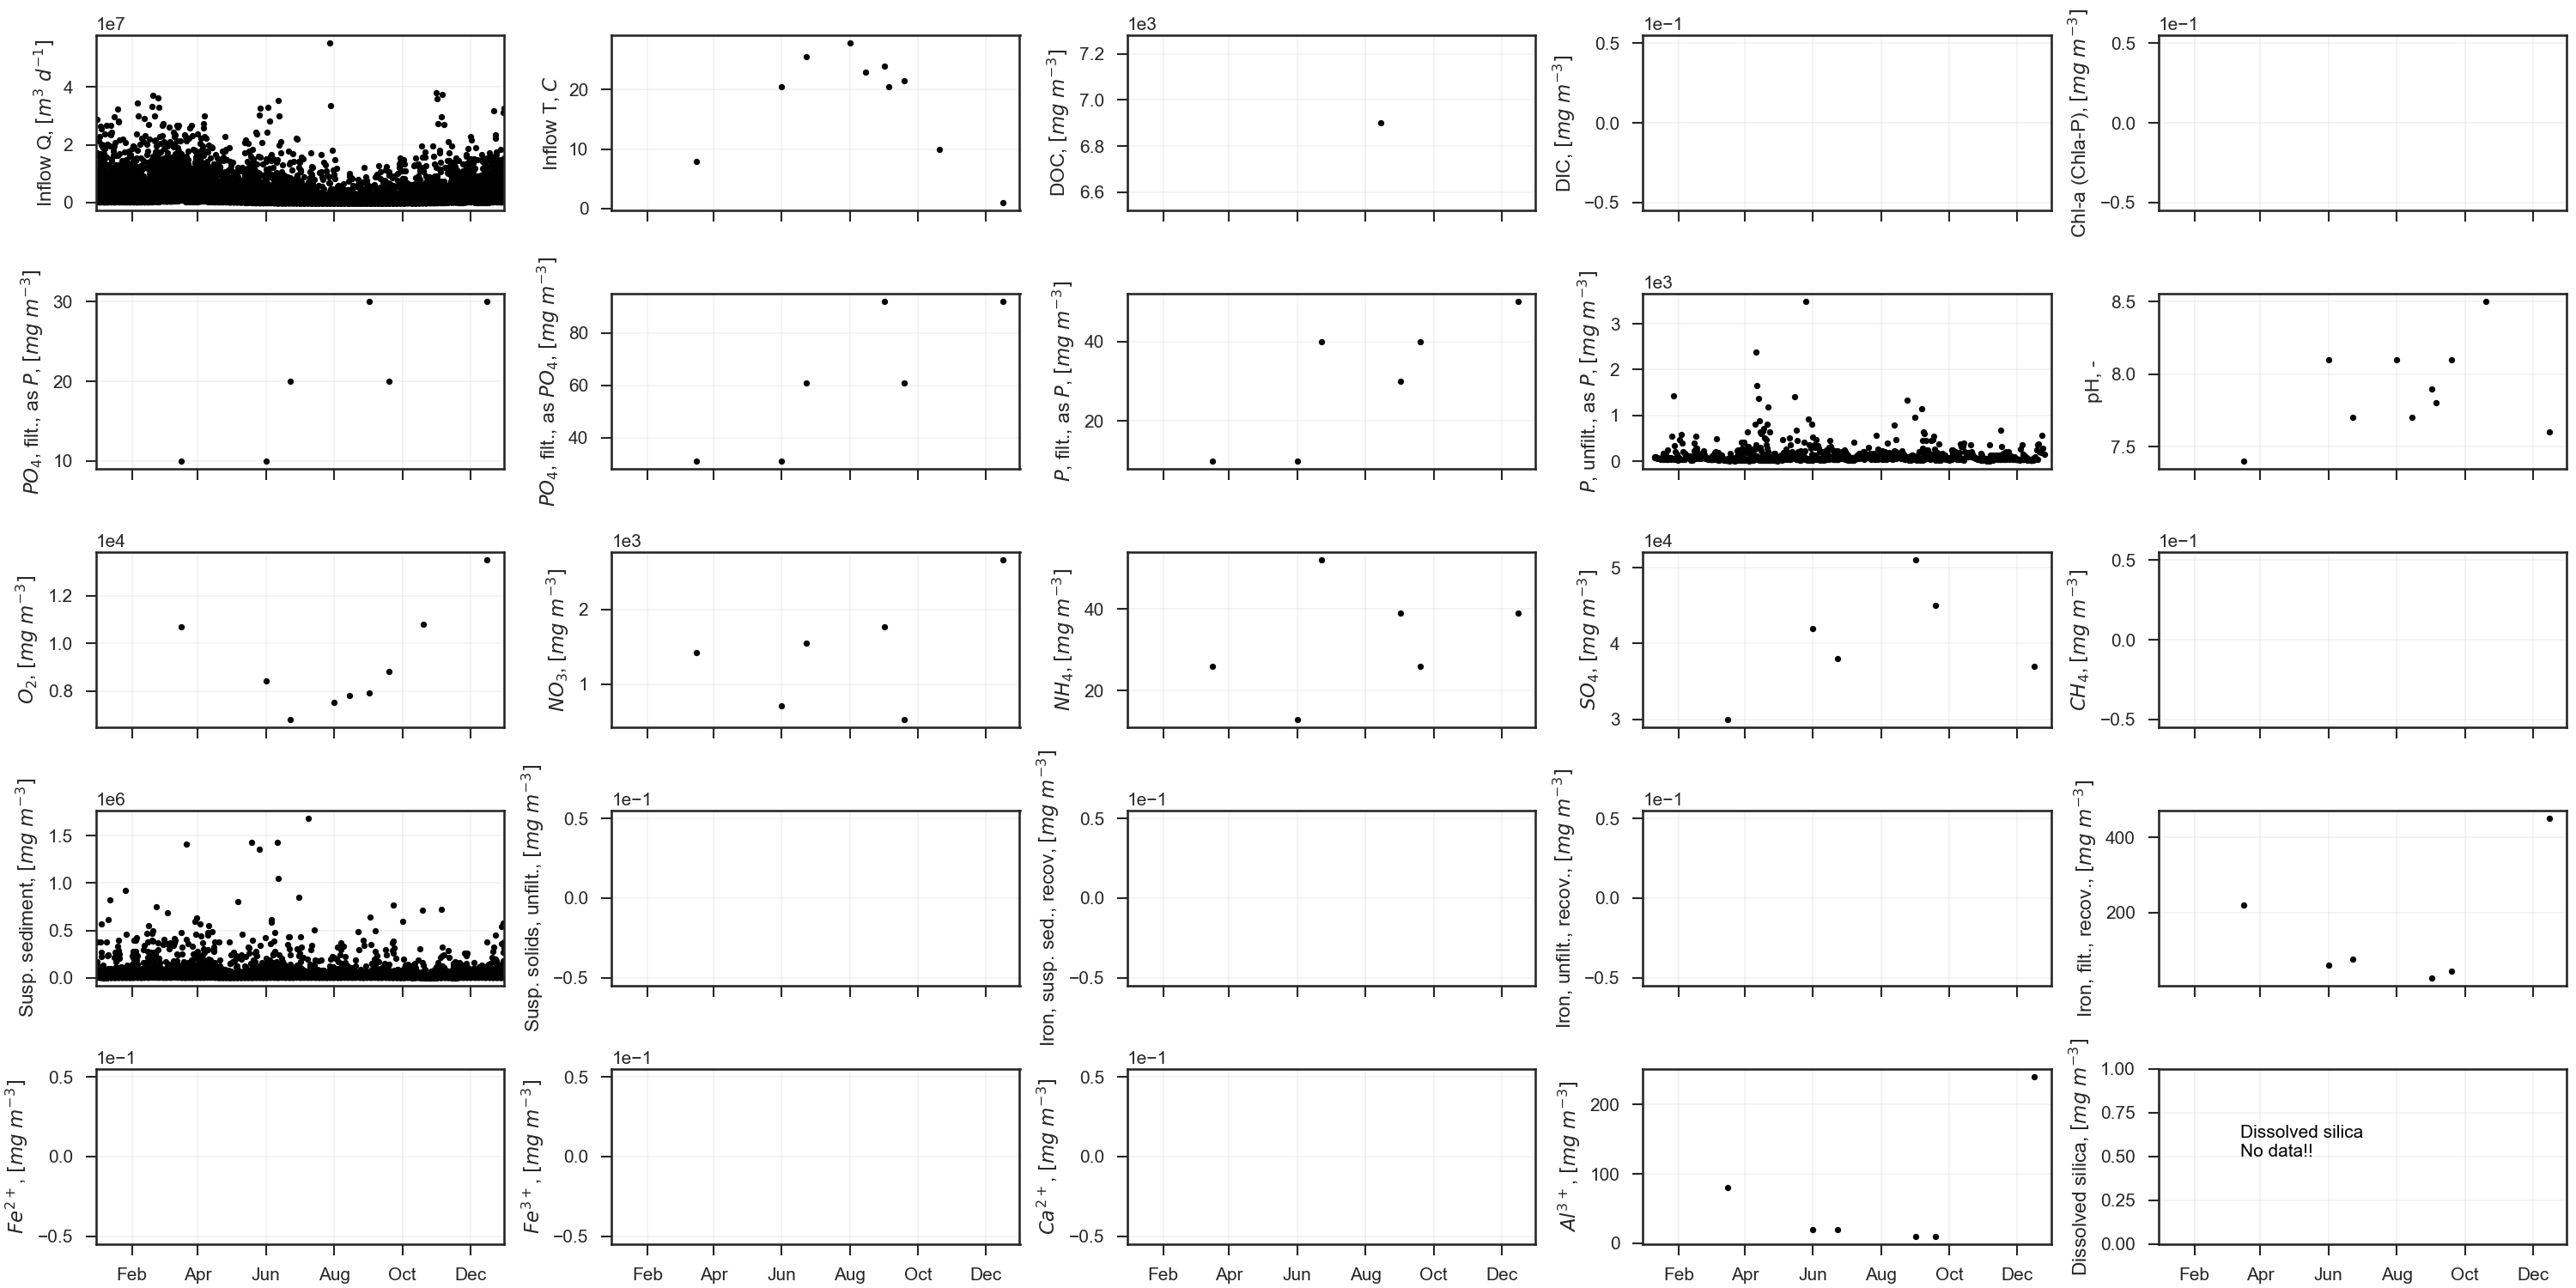
\includegraphics[width=\textwidth]{rivers/Central basin/plot_1yr grandriver.png}
\end{figure}
\end{frame}

\begin{frame}
\frametitle{Central Basin: Rocky river}
\begin{figure}
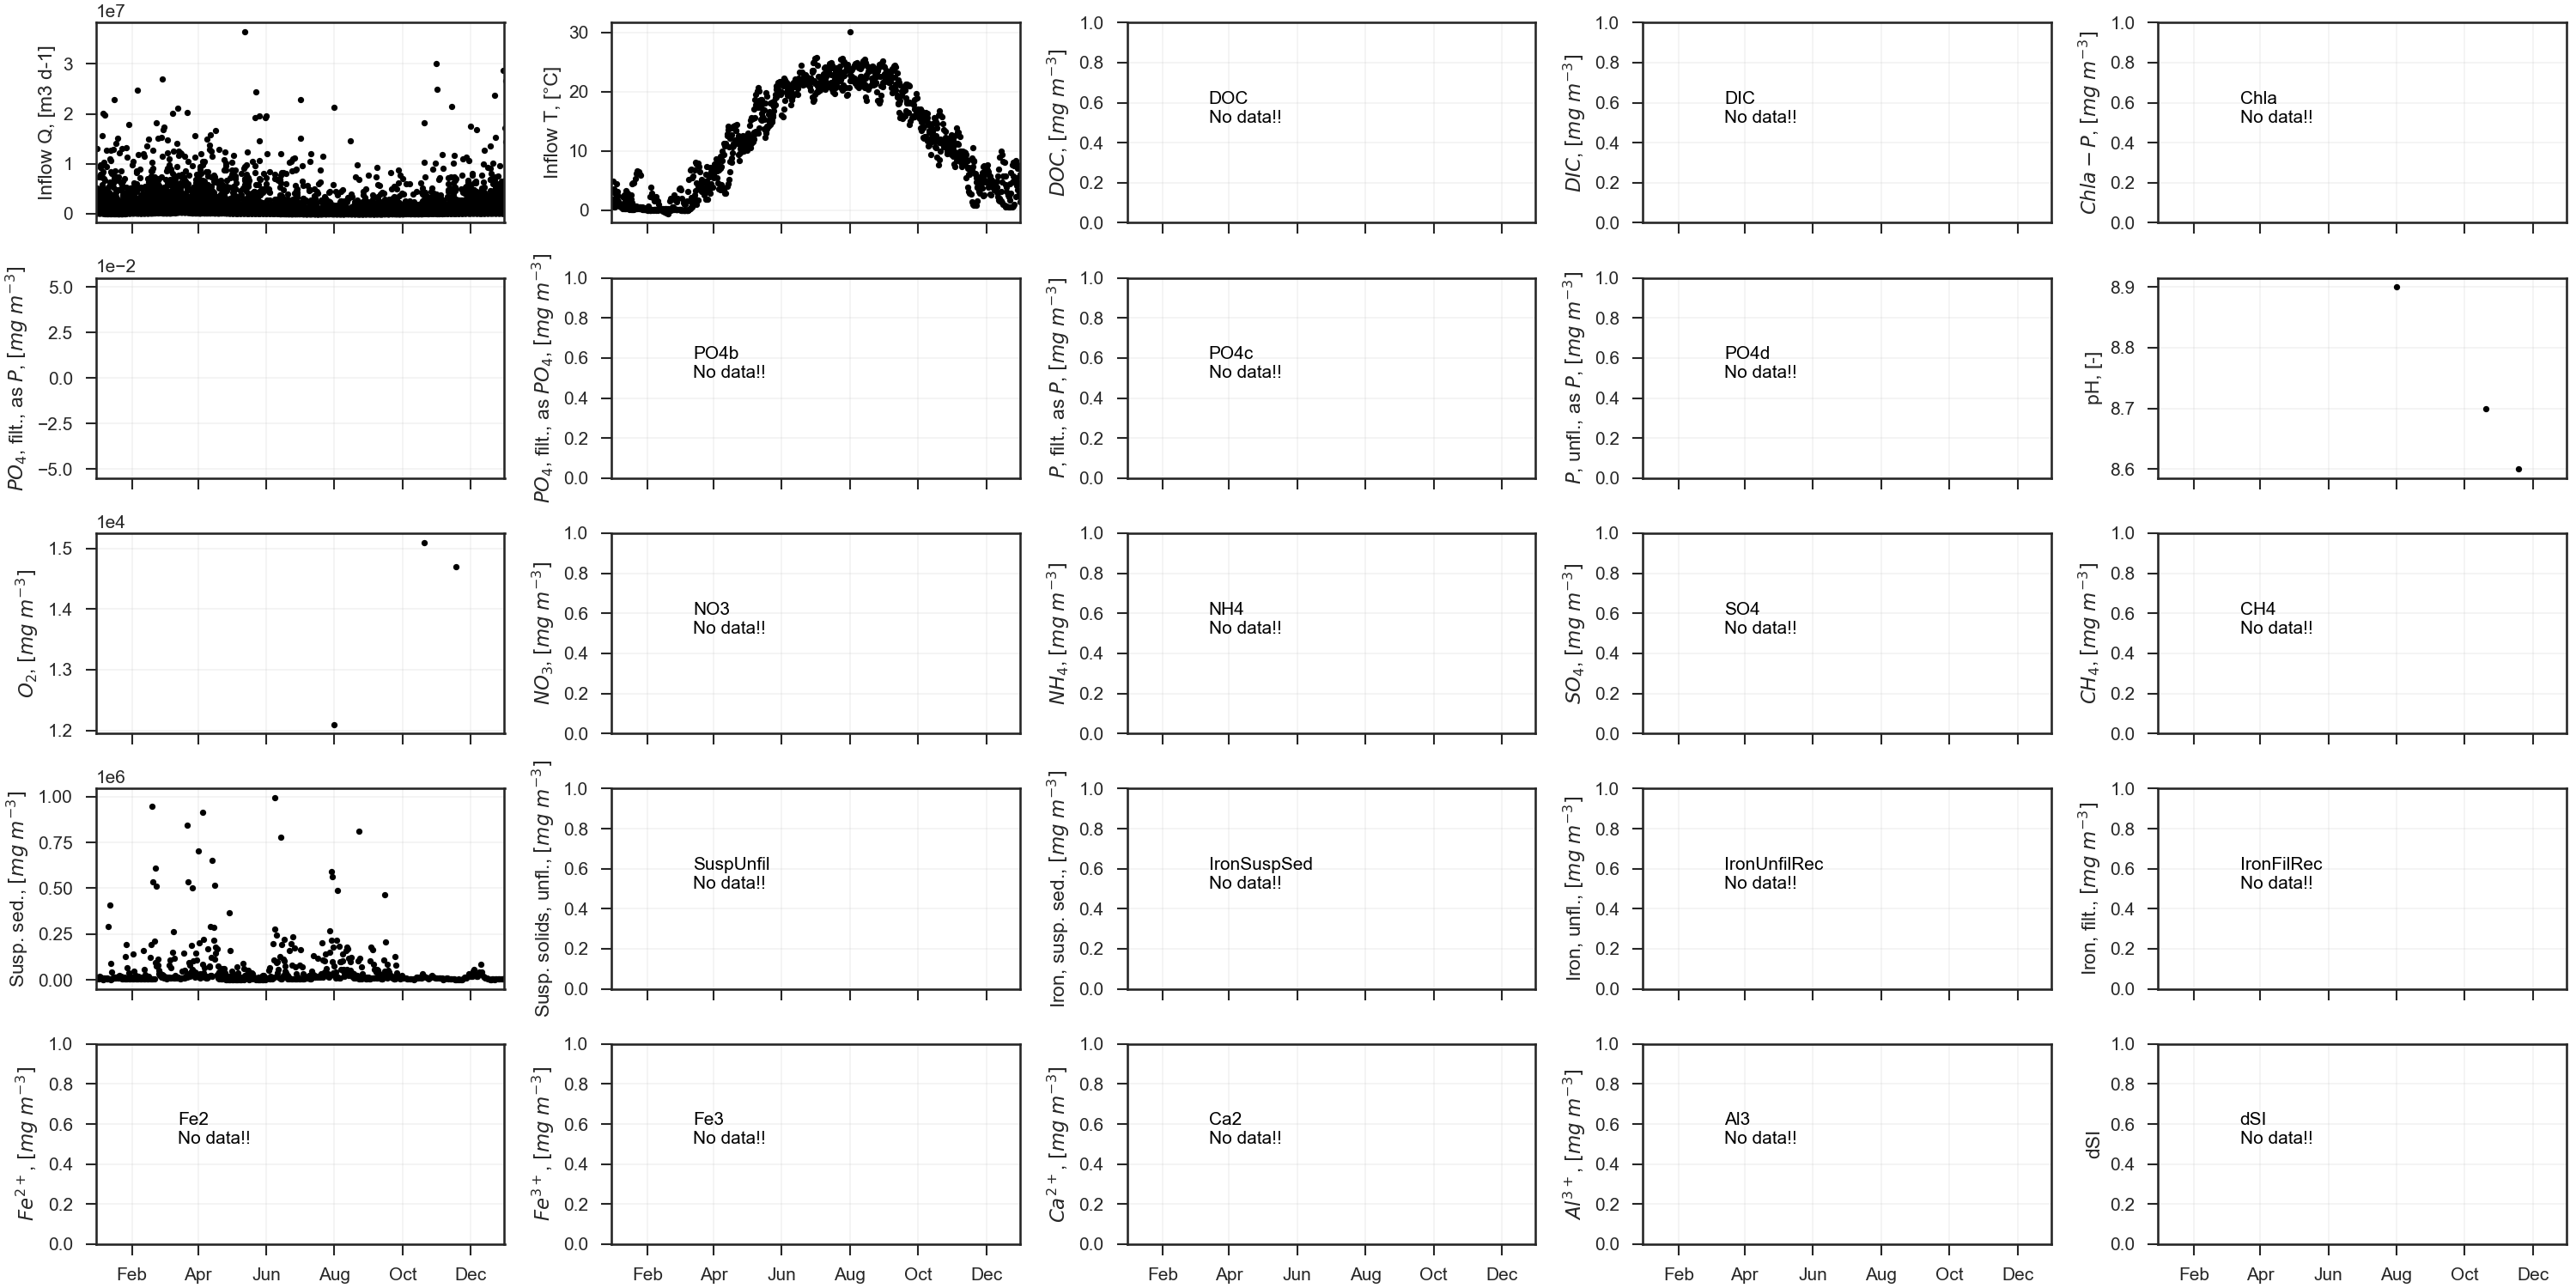
\includegraphics[width=\textwidth]{rivers/Central basin/plot_1yr rockyriver.png}
\end{figure}
\end{frame}

\begin{frame}
\frametitle{Central Basin: Sandusky river}
\begin{figure}
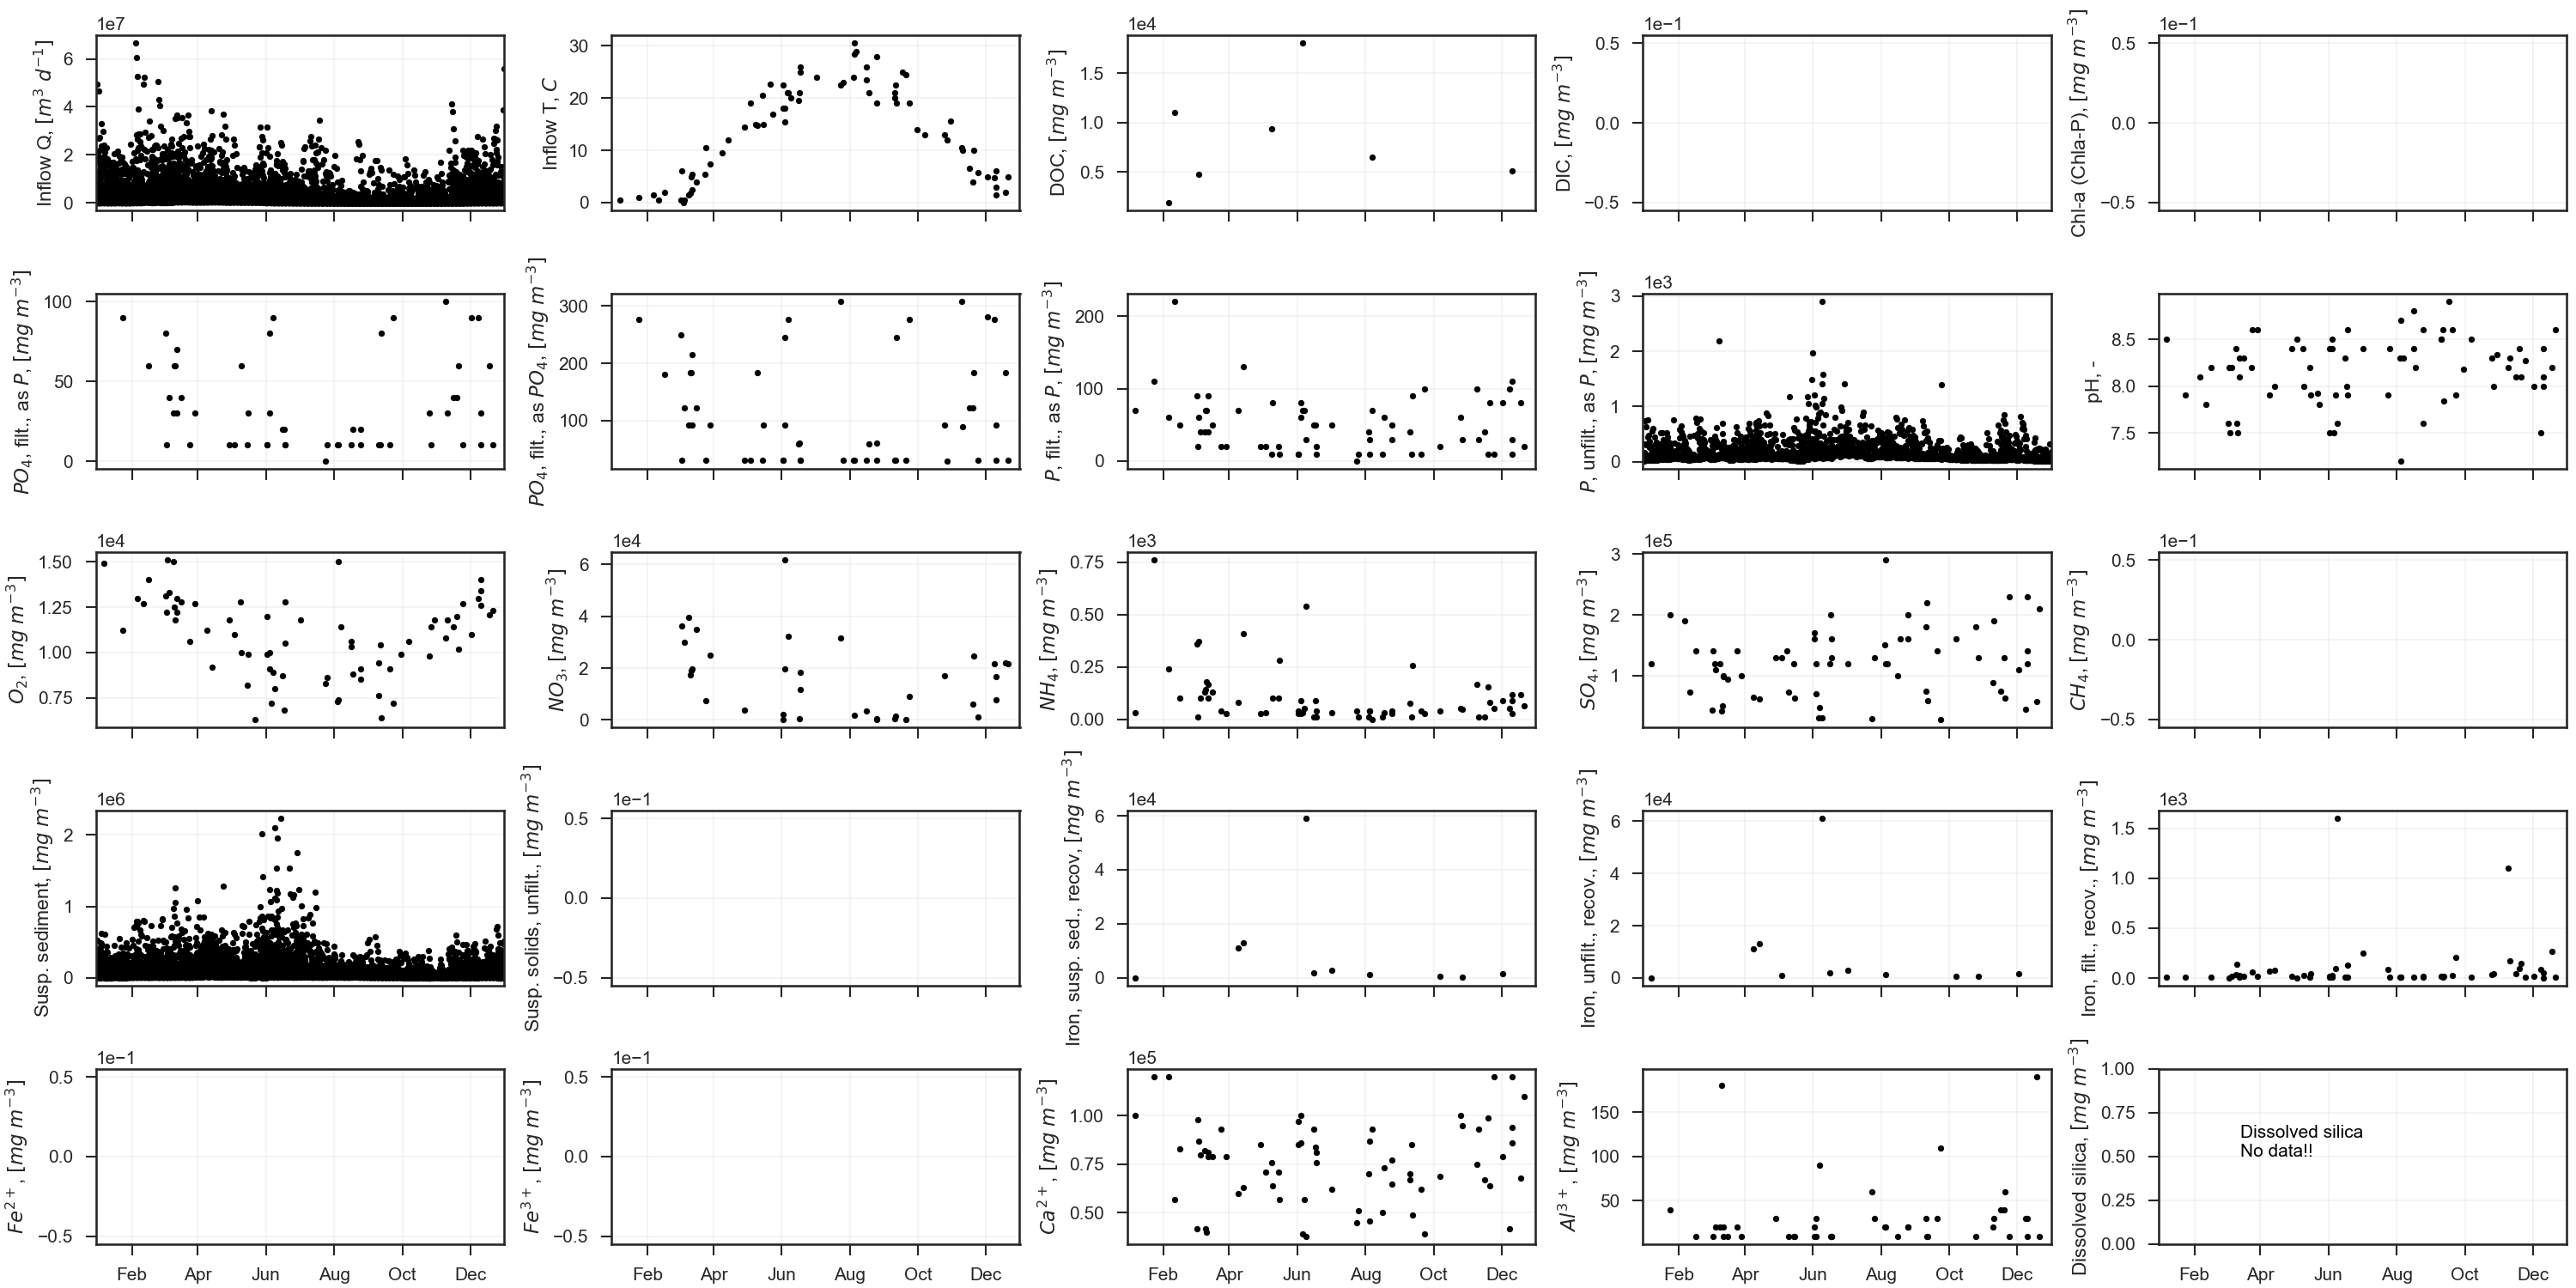
\includegraphics[width=\textwidth]{rivers/Central basin/plot_1yr sanduskyriver.png}
\end{figure}
\end{frame}

\begin{frame}
\frametitle{Central Basin: South-western Huron river}
\begin{figure}
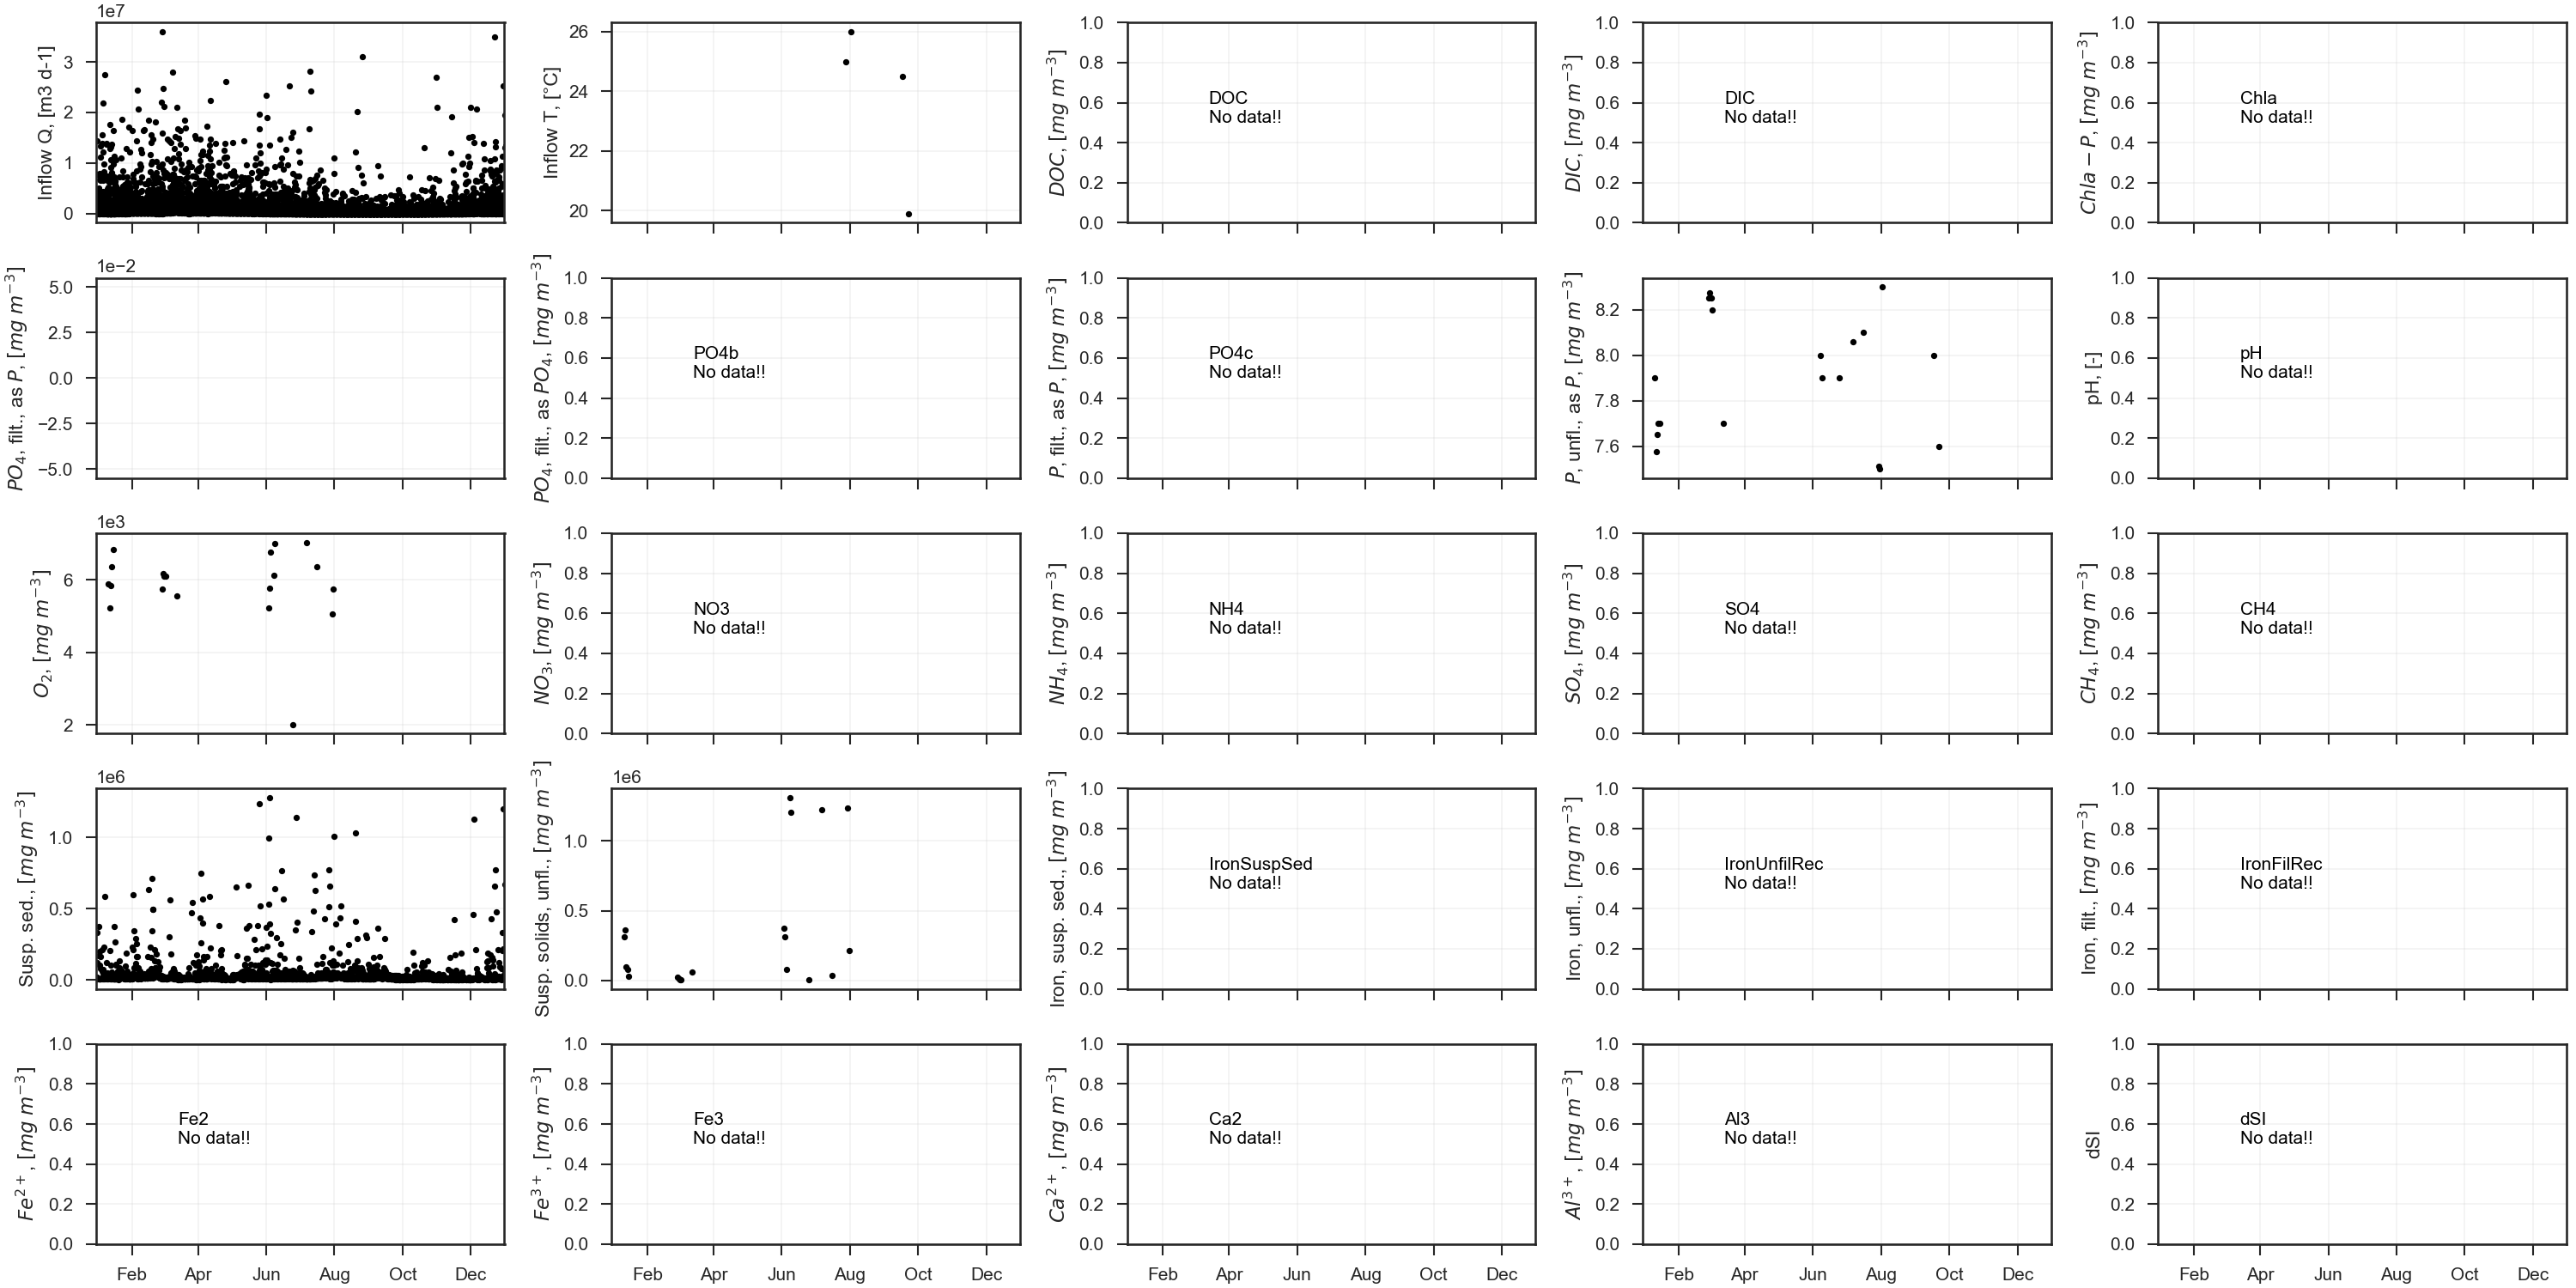
\includegraphics[width=\textwidth]{rivers/Central basin/plot_1yr southwesternhuronriver.png}
\end{figure}
\end{frame}

\begin{frame}
\frametitle{Central Basin: Vermillion river}
\begin{figure}
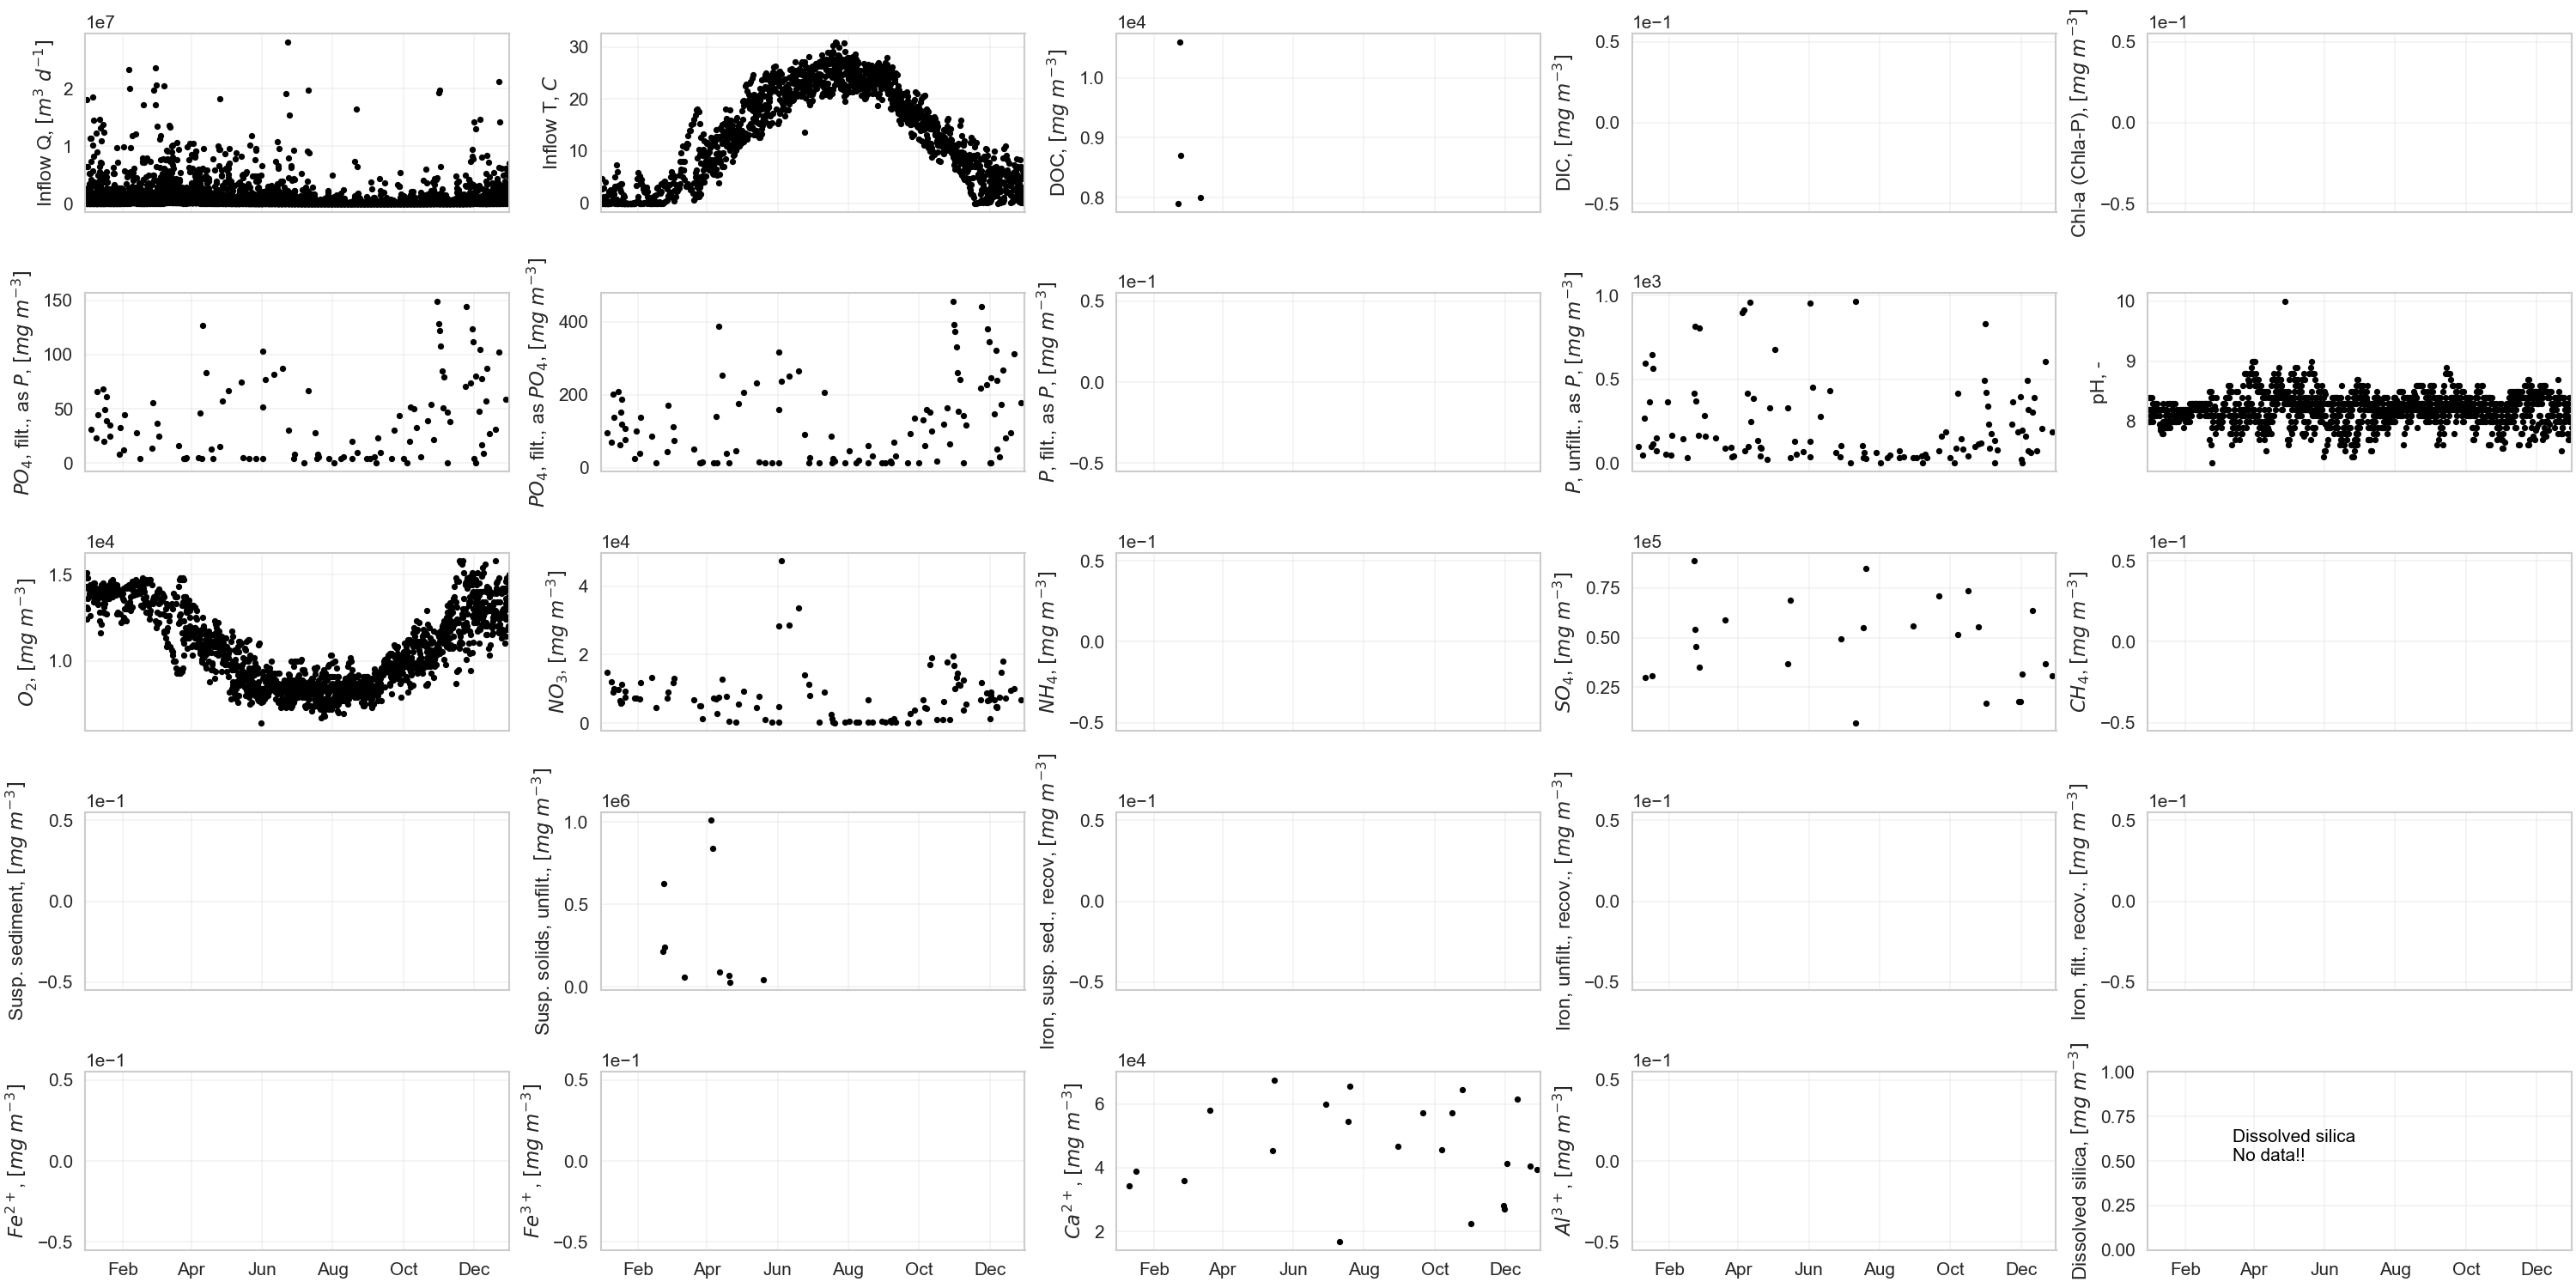
\includegraphics[width=\textwidth]{rivers/Central basin/plot_1yr vermillion.png}
\end{figure}
\end{frame}


\subsection{Eastern Basin}
\label{sub:eastern_basin}


\begin{frame}
\frametitle{Eastern Basin: Niagara river}
\begin{figure}
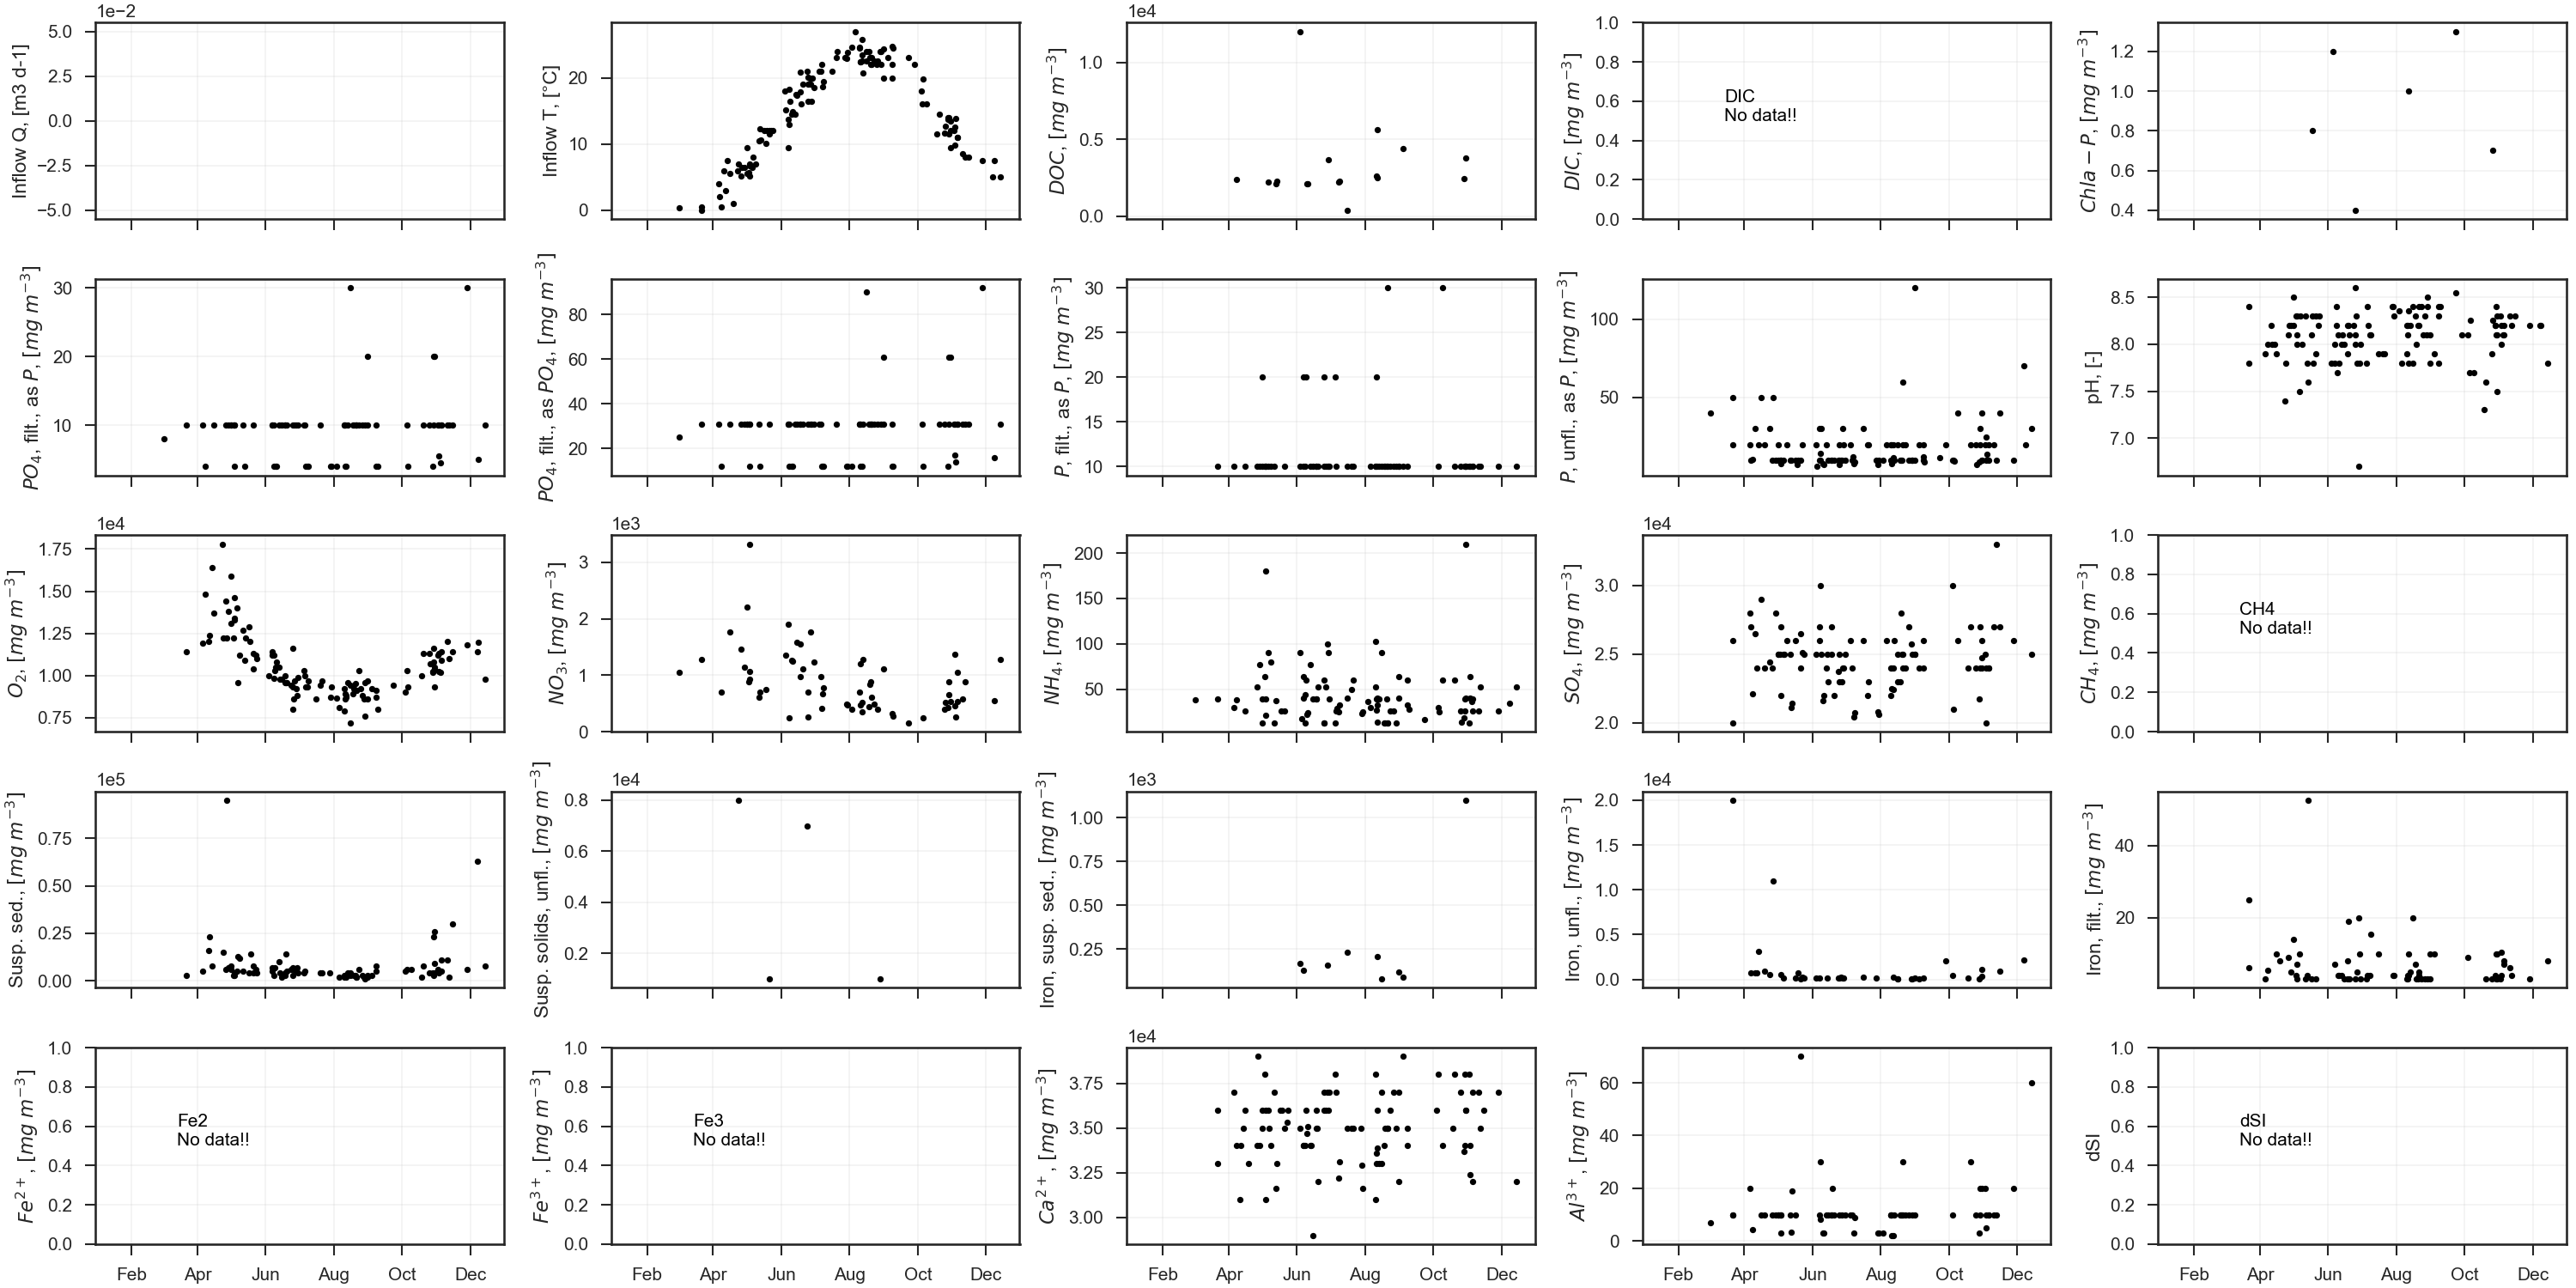
\includegraphics[width=\textwidth]{rivers/Eastern basin/plot_1yr niagarariver.png}
\end{figure}
\end{frame}

\begin{frame}
\frametitle{Eastern Basin: Buffalo creek}
\begin{figure}
\includegraphics[width=\textwidth]{rivers/Eastern basin/plot_1yr Buffalocreek.png}
\end{figure}
\end{frame}

\begin{frame}
\frametitle{Eastern Basin: Cattaraugus creek}
\begin{figure}
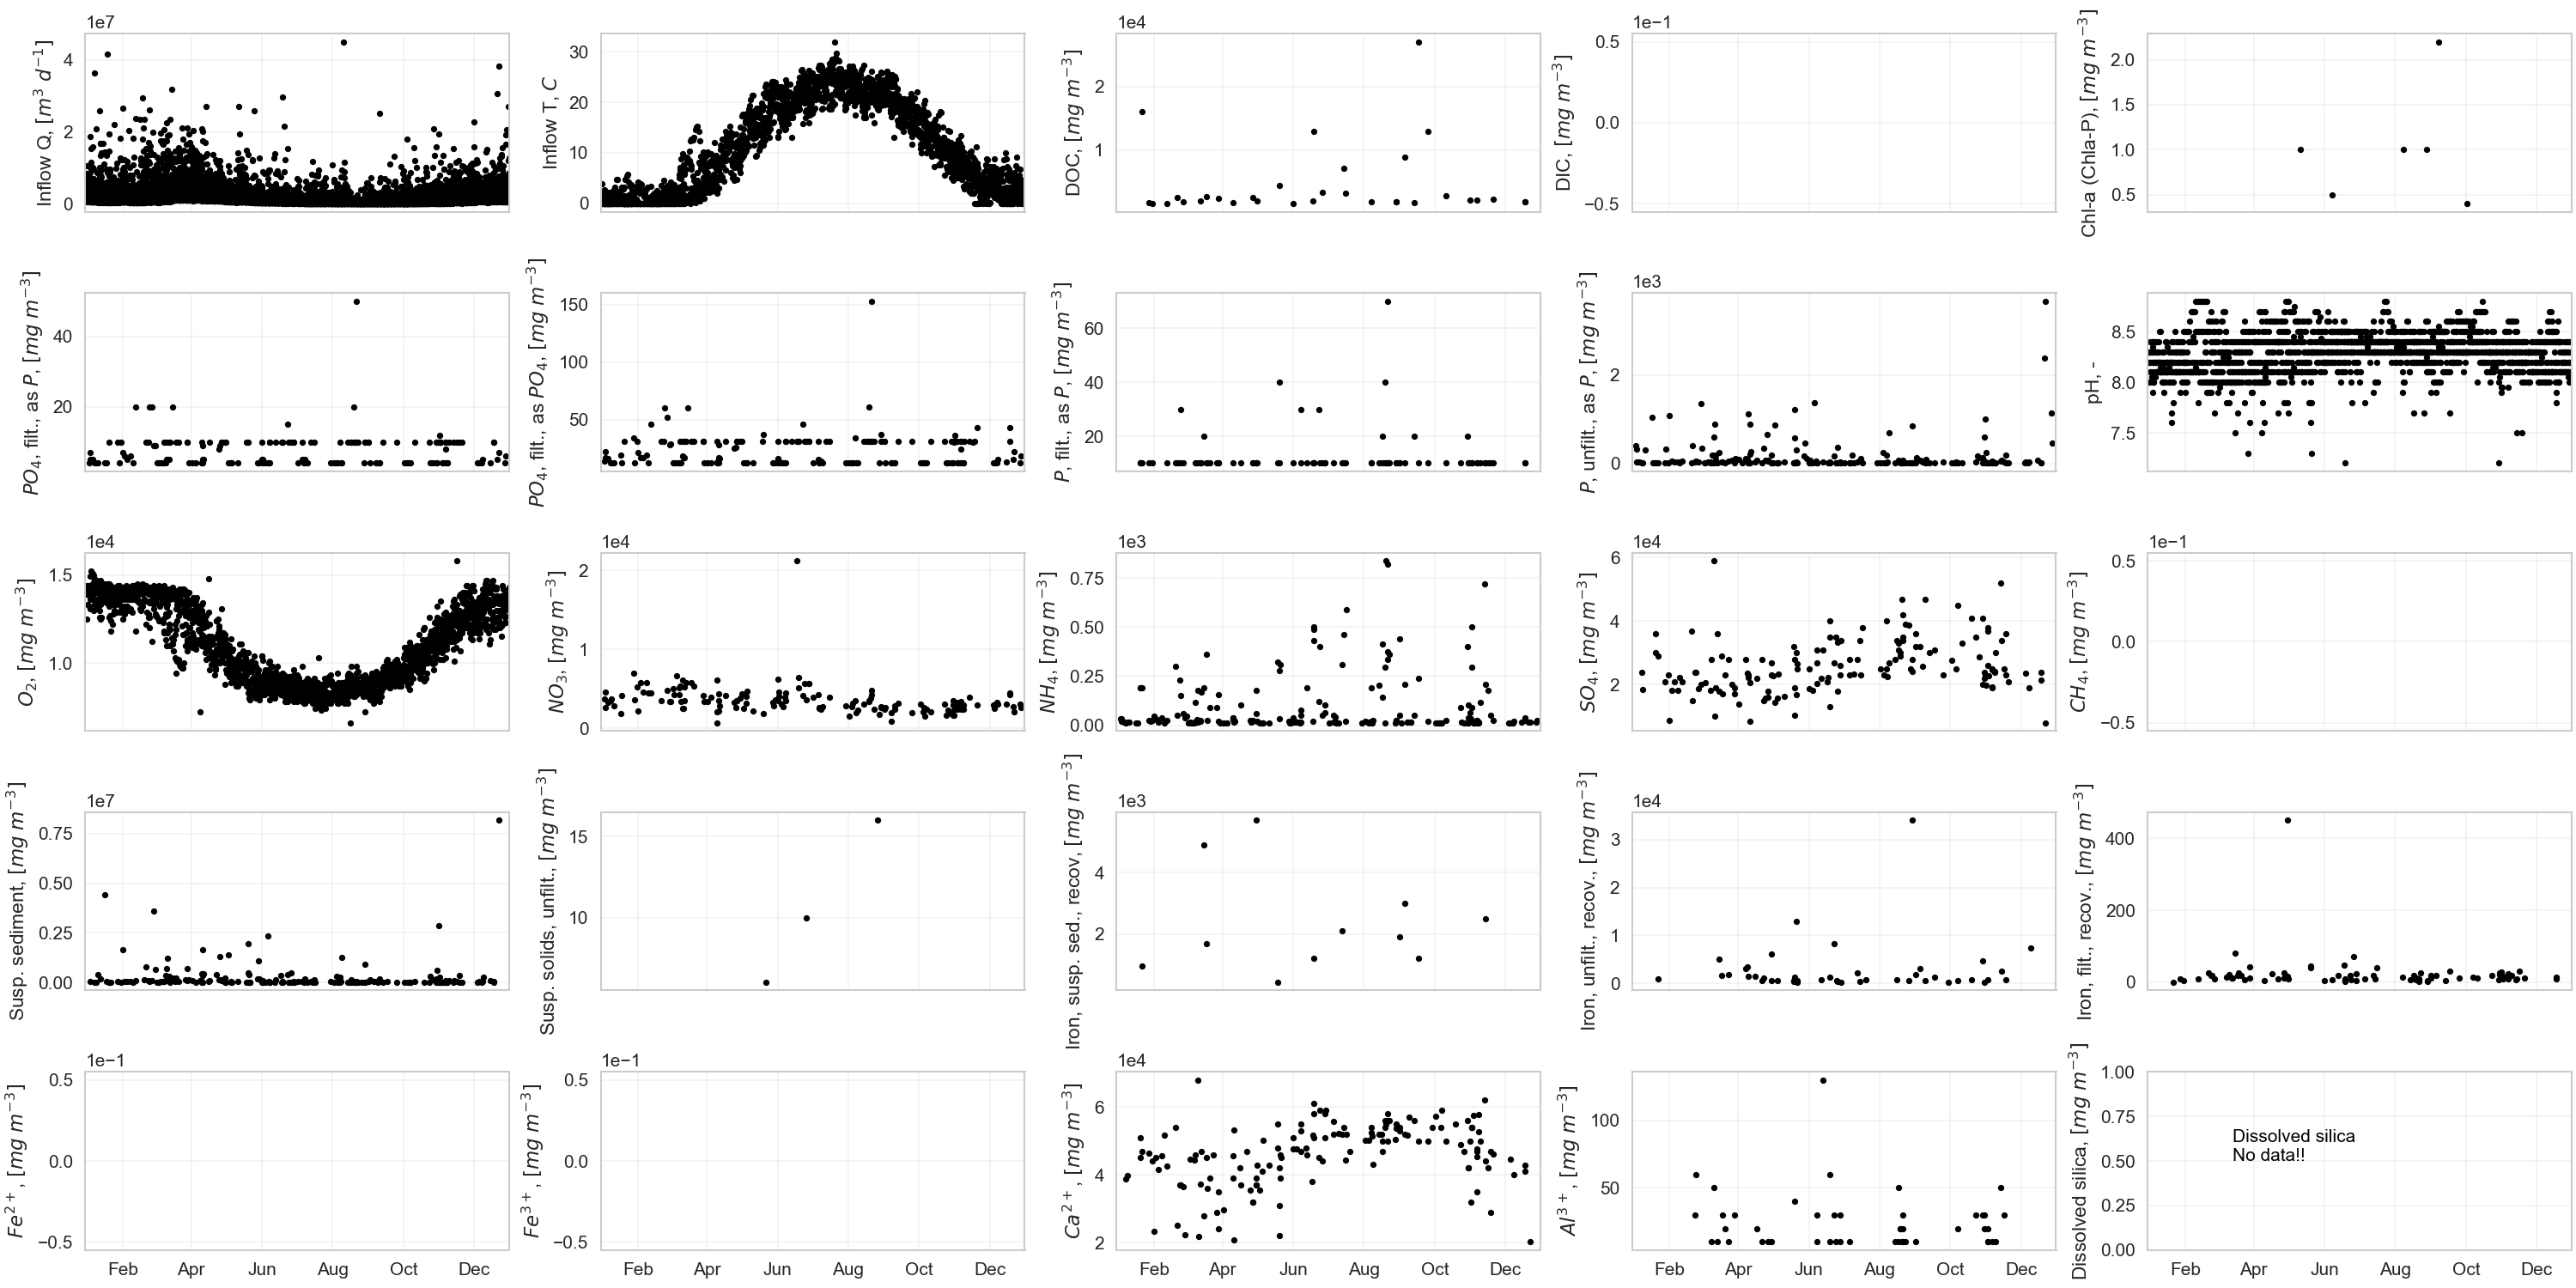
\includegraphics[width=\textwidth]{rivers/Eastern basin/plot_1yr cattarauguscreek.png}
\end{figure}
\end{frame}



\section{US Rivers' Combined data}
\label{sec:us_rivers_combined_data}



\end{document}
